\documentclass[12pt]{report}
%\documentclass[12pt,twoside]{report}
\usepackage[utf8]{inputenc}
\usepackage{textcomp}
\usepackage{tabularx}
\usepackage{graphicx}
\graphicspath{ {images/} }
\usepackage[a4paper,left=1.5in,right=1in,top=1in,bottom=1in]{geometry}
\usepackage{fancyhdr}
\pagestyle{fancy}
\usepackage{caption}
\usepackage{subcaption}
\usepackage{setspace}
\usepackage{amsmath}
\usepackage{esint}
\usepackage{accents}
\usepackage{bm}
\usepackage{textcomp}
\usepackage{mathtools}
\usepackage{siunitx}
\usepackage{placeins}
\usepackage{dotlessi}
\usepackage{hyperref}
\usepackage{float}


\usepackage[toc,page]{appendix}
%\usepackage[titletoc]{appendix}

\usepackage[style=ieee,]{biblatex}
\addbibresource{testReferences.bib}
\addbibresource{Impedance Spectroscopy.bib}

\usepackage[scaled]{helvet}
\renewcommand\familydefault{\sfdefault} 
\usepackage[T1]{fontenc}


\usepackage{titlesec}

\titleformat{\section}
    {\normalfont\bfseries}
    {\thesection}{1em}{}

\titleformat{\chapter}
    {\normalfont\bfseries\centering}
    {Chapter \thechapter:}{1em}{}
\titlespacing{\chapter}{0pt}{*1}{*2}

\titleformat{\subsection}
    {\normalfont\bfseries\itshape}
    {\thesubsection}{1em}{}
    

    
%\titlespacing{\chapter}{0pt}{*4}{1.5}

\newcommand{\Tau}{\mathcal{T}}

\DeclareMathOperator{\arccosh}{arccosh}
\DeclareMathOperator{\arcsinh}{arcsinh}
\DeclareMathOperator{\arctanh}{arctanh}
\DeclareMathOperator{\Log}{Log}


\setcounter{secnumdepth}{3}

\pagenumbering{roman}

\title{Single Cell Impedance Spectroscopy}
\author{David Lange}
\date{April 2019}

\begin{document}
%\begin{titlepage}
\begin{center}
\vspace*{1cm}

\large SINGLE-CELL IMPEDANCE SPECTROSCOPY

\vfill

A Thesis\\
presented to\\
the Faculty of California Polytechnic State University,\\
San Luis Obispo\\

\vfill

In Partial Fulfillment\\
of the Requirements for the Degree\\
Master of Science in Biomedical Engineering\\

\vspace{0.75 in}

by\\
David Paul Lange\\
November 2019
\vspace{1.5 in}
    
    
\end{center}
\end{titlepage}

%\thispagestyle{plain}
\begin{center}
    \mbox{}
    \vfill
    \textcopyright \; 2019\\
    David Paul Lange\\
    ALL RIGHTS RESERVED
\end{center}

%\chapter*{COMMITTEE MEMBERSHIP}
%\vspace{0.5 in}

\begin{tabular}{r l}
    TITLE:\;\;\;\;\; & Single Cell Impedance Spectroscopy\\
    \\
    \\
    AUTHOR:\;\;\;\;\; & David Paul Lange\\
    \\
    \\
    DATE SUBMITTED:\;\;\;\;\;\; & November 2019\\
    \\
    \\
    \\
    \\
    \\
    \\
    \\
    \\
    \\
    \\
    \\
    COMMITTEE CHAIR:\;\;\;\;\; & David Clague Ph.D.\\ 
    \;\;\;\;\; & Professor of Biomedical Engineering\\
    \\
    \\
    \\
    COMMITTEE MEMBER: \;\;\;\;\; & Benjamin Hawkins Ph.D\\
    \;\;\;\;\; & Assistant Professor of Biomedical Engineering\\
    \\
    \\
    \\
    COMMITTEE MEMBER: \;\;\;\;\; & \\
    \;\;\;\;\; & Professor of \\
    \\
    \\
    \\
    COMMITTEE MEMBER: \;\;\;\;\; & \\
    \;\;\;\;\; & Professor of \\
\end{tabular}






%\chapter*{ABSTRACT}
%
\par Impedance spectroscopy (IS) is an important tool for cell detection and characterization in medical and food safety applications. In this thesis, the Cal Poly Biofluidics Lab's impedance spectroscopy system was re-evaluated and optimized for single-cell impedance spectroscopy. To evaluate the IS system, an impedance spectroscopy bioMEMS chip was fabricated in the Cal Poly Microfabcrication lab, software was developed to run IS experiments, and studies were run to validate the system. To explore IS optimization, Maxwell's mixture theorem and the Schwartz-Christoffel transform was used to calculate an analytic impedance solution to the co-planar electrode system, a novel volume fraction to account for the non-uniformity of the electric field was developed to increase the accuracy of the analytic solution and to investigate the effect of cell position on the impedance spectrum, a software program was created to allow easy access to the analytic solution, and FEA models were developed to compare to the analytic solution and to investigate the effect of complex device geometry.





%\chapter*{ACKNOWLEDGEMENTS}
%
\mbox

\\
\par First, I want to thank my family and friends who have showed their unfettering support. I can always count on their support when the going gets tough.

\vfill

\par To the committee members, thank you for your time in considering this thesis.  

\vfill

\par I'd like to thank Hans Mayer for his training and aide in the soft-lithography manufacturing process.

\vfill

\par I'd also like to thank Jack Foley whose companionship and collaboration inside the clean room was critical for delivering for fabricating a functional device. 

\vfill

\par I want to make a special thank you to Dr. Ben Hawkins. Without his time resources, and support, the device would not have been able to be fabricated at Cal Poly. It has been a pleasure to spend those long hours in the clean room with you.

\vfill

\par I'd also like to make a special thank you to Dr.Clague for
\\


\tableofcontents

\listoffigures

\listoftables

\doublespacing

%\chapter{Test}
% \section{Testing} \par Lines five and six add some text about the chapter and author into the footer again in different places depending on whether the page is odd or even. Now if we compile the document with this code in we can see the headers and footers have been added in: Lines five and six add some text about the chapter and author into the footer again in different places depending on whether the page is odd or even. Now if we compile the document with this code in we can see the headers and footers have been added in: Lines five and six add some text about the chapter and author into the footer again in different places depending on whether the page is odd or even \ref{fig: awesome_view} \cite{einstein}.
 
 \begin{figure}[h]
 \centering
 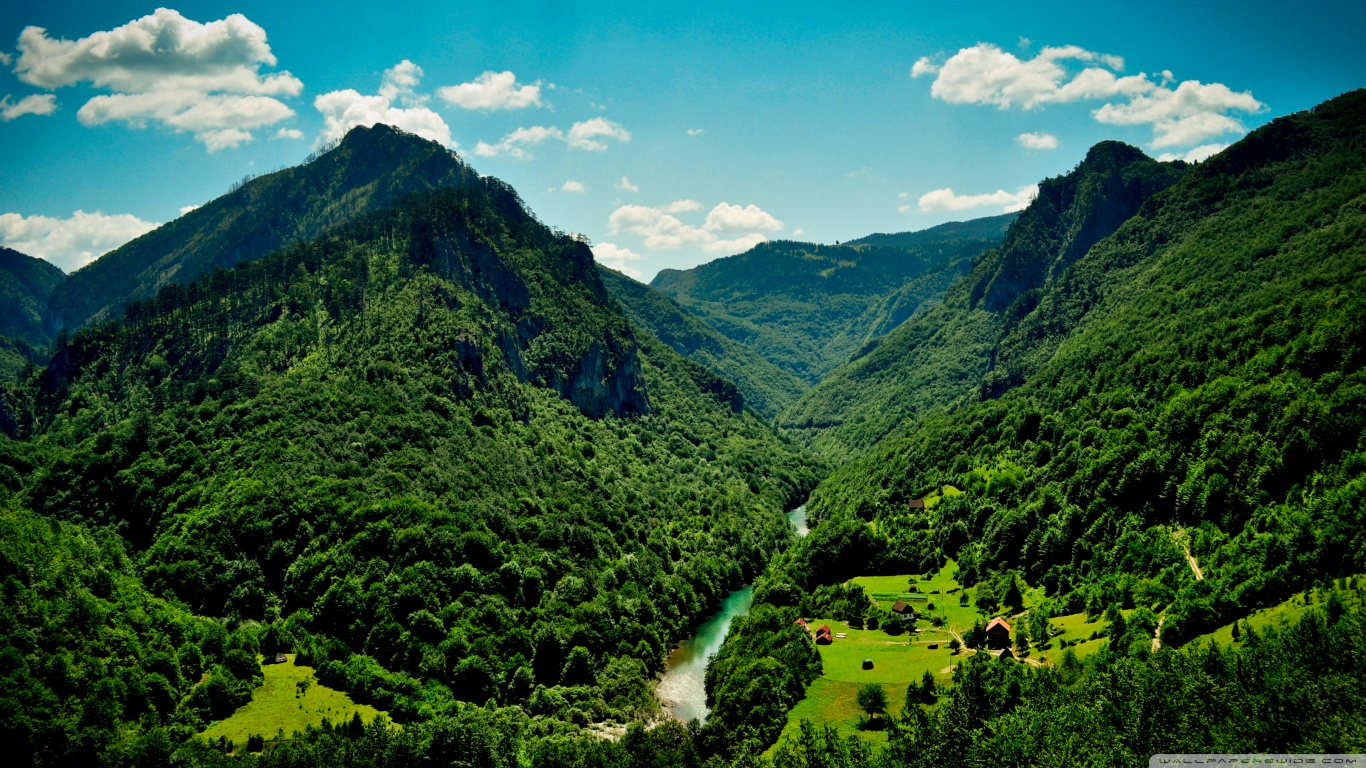
\includegraphics[width=0.5\textwidth]{awesome_view.jpg}
 \caption{An amazing view}
 \label{fig: awesome_view}
 \end{figure}
 
 \par Now if we compile the document with this code in we can see the headers and footers have been added in: Lines five and six add some text about the chapter and author into the footer again in different places depending on whether the page is odd or even. Now if we compile the document with this code in we can see the headers and footers have been added in: Lines five and six add some text about the chapter and author into the footer again in different places depending on whether the page is odd or even. Now if we compile the document with this code in we can see the headers and footers have been added in: Lines five and six add some text about the chapter and author into the footer again in different places depending on whether the page is odd or even. Now if we compile the document with this code in we can see the headers and footers have been added in: Lines five and six add some text about the chapter and author into the footer again in different places depending on whether the page is odd or even. Now if we compile the document with this code in we can see the headers and footers have been added in: Lines five and six add some text about the chapter and author into the footer again in different places depending on whether the page is odd or even. Now if we compile the document with this code in we can see the headers and footers have been added in: Lines five and six add some text about the chapter and author into the footer again in different places depending on whether the page is odd or even. Now if we compile the document with this code in we can see the headers and footers have been added in: Lines five and six add some text about the chapter and author into the footer again in different places depending on whether the page is odd or even. Now if we compile the document with this code in we can see the headers and footers have been added in: Lines five and six add some text about the chapter and author into the footer again in different places depending on whether the page is odd or even. Now if we compile the document with this code in we can see the headers and footers have been added in: Lines five and six add some text about the chapter and author into the footer again in different places depending on whether the page is odd or even. Now if we compile the document with this code in we can see the headers and footers have been added in: Lines five and six add some text about the chapter and author into the footer again in different places depending on whether the page is odd or even.
 
 
 \begin{table}[h]
\centering
\begin{tabular}{l | l | l}
A & B & C \\
\hline
1 & 2 & 3 \\
4 & 5 & 6
\end{tabular}
\caption{very basic table}
\label{tab:abc}
\end{table}

 \par Now if we compile the document with this code in we can see the headers and footers have been added in: Lines five and six add some text about the chapter and author into the footer again in different places depending on whether the page is odd or even. Now if we compile the document with this code in we can see the headers and footers have been added in: Lines five and six add some text about the chapter and author into the footer again in different places depending on whether the page is odd or even. Now if we compile the document with this code in we can see the headers and footers have been added in: Lines five and six add some text about the chapter and author into the footer again in different places depending on whether the page is odd or even. Now if we compile the document with this code in we can see the headers and footers have been added in: Lines five and six add some text about the chapter and author into the footer again in different places depending on whether the page is odd or even. Now if we compile the document with this code in we can see the headers and footers have been added in: Lines five and six add some text about the chapter and author into the footer again in different places depending on whether the page is odd or even. Now if we compile the document with this code in we can see the headers and footers have been added in: Lines five and six add some text about the chapter and author into the footer again in different places depending on whether the page is odd or even. Now if we compile the document with this code in we can see the headers and footers have been added in: Lines five and six add some text about the chapter and author into the footer again in different places depending on whether the page is odd or even. Now if we compile the document with this code in we can see the headers and footers have been added in: Lines five and six add some text about the chapter and author into the footer again in different places depending on whether the page is odd or even. Now if we compile the document with this code in we can see the headers and footers have been added in: Lines five and six add some text about the chapter and author into the footer again in different places depending on whether the page is odd or even. Now if we compile the document with this code in we can see the headers and footers have been added in: Lines five and six add some text about the chapter and author into the footer again in different places depending on whether the page is odd or even. Now if we compile the document with this code in we can see the headers and footers have been added in: Lines five and six add some text about the chapter and author into the footer again in different places depending on whether the page is odd or even. Now if we compile the document with this code in we can see the headers and footers have been added in: Lines five and six add some text about the chapter and author into the footer again in different places depending on whether the page is odd or even. Now if we compile the document with this code in we can see the headers and footers have been added in: Lines five and six add some text about the chapter and author into the footer again in different places depending on whether the page is odd or even. Now if we compile the document with this code in we can see the headers and footers have been added in: Lines five and six add some text about the chapter and author into the footer again in different places depending on whether the page is odd or even. 
 
  \begin{figure}[h]
    \centering
    \begin{subfigure}[b]{0.45\textwidth}
        \centering
        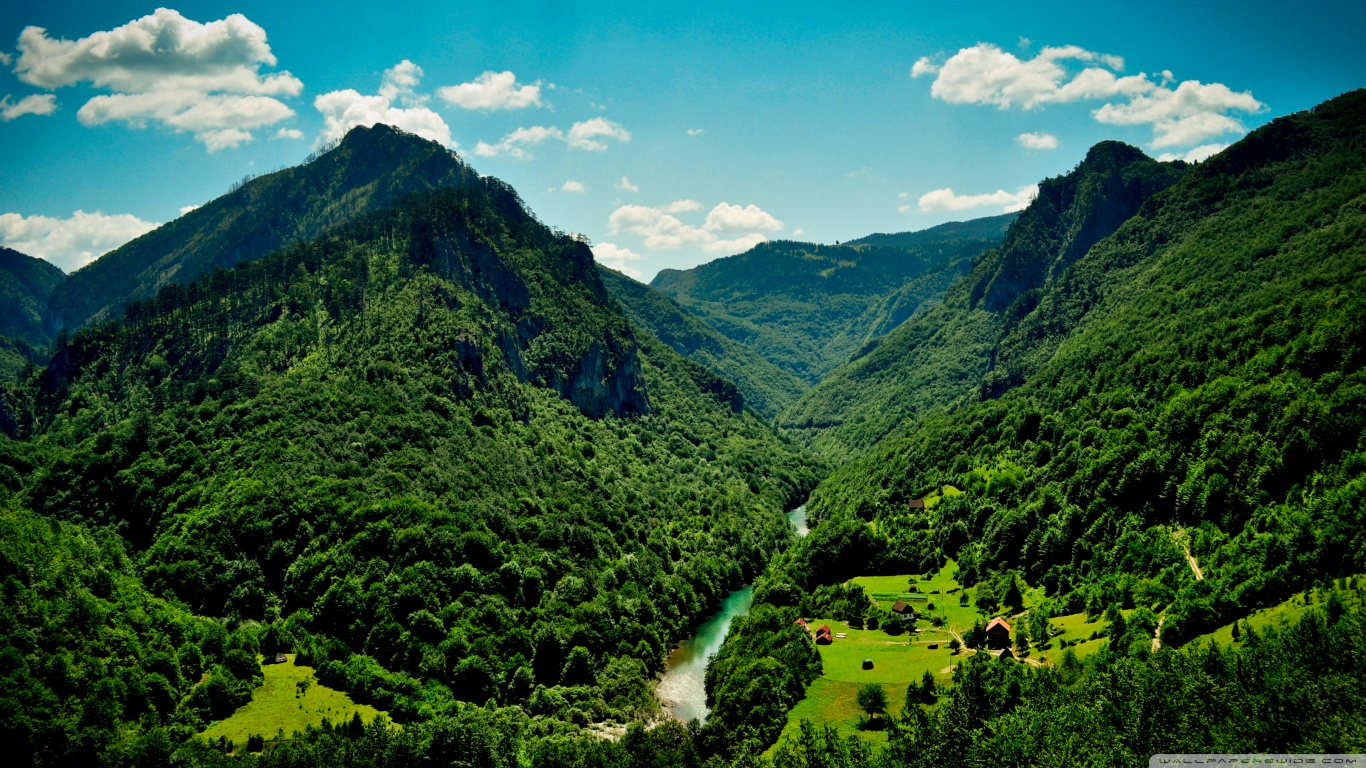
\includegraphics[width=\textwidth]{awesome_view}
        \caption{This is another awesome view}
        \label{fig:another_awesome_view_a}
    \end{subfigure}
    \hfill
    \begin{subfigure}[b]{0.45\textwidth}
        \centering
        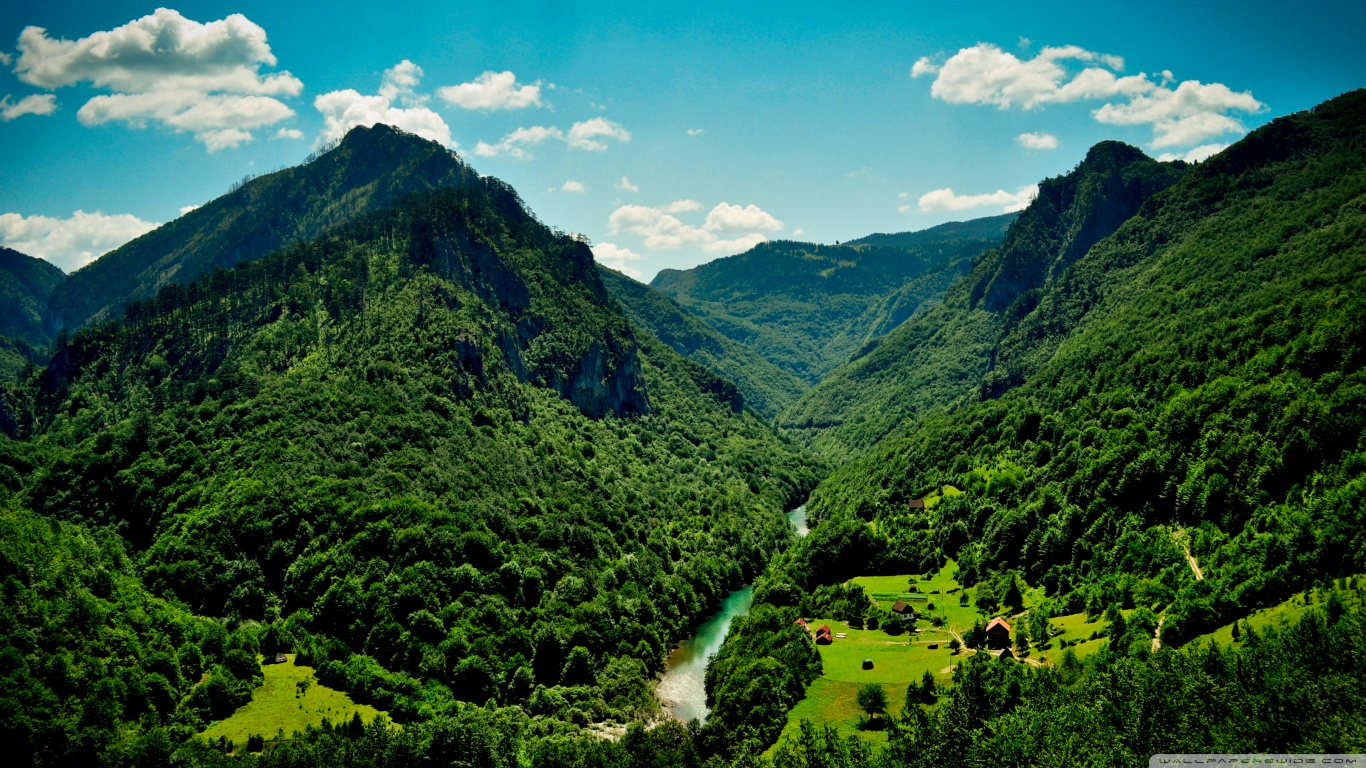
\includegraphics[width=\textwidth]{awesome_view}
        \caption{Yet another awesome view}
        \label{fig:another_awesome_view_b}
    \end{subfigure} 
    \caption{Two awesome pictures}
    \label{fig:two_awesome_pictures}
 \end{figure}
 
 \par Now if we compile the document with this code in we can see the headers and footers have been added in: Lines five and six add some text about the chapter and author into the footer again in different places depending on whether the page is odd or even. Now if we compile the document with this code in we can see the headers and footers have been added in: Lines five and six add some text about the chapter and author into the footer again in different places depending on whether the page is odd or even. Now if we compile the document with this code in we can see the headers and footers have been added in: Lines five and six add some text about the chapter and author into the footer again in different places depending on whether the page is odd or even. Now if we compile the document with this code in we can see the headers and footers have been added in: Lines five and six add some text about the chapter and author into the footer again in different places depending on whether the page is odd or even. Now if we compile the document with this code in we can see the headers and footers have been added in: Lines five and six add some text about the chapter and author into the footer again in different places depending on whether the page is odd or even. Now if we compile the document with this code in we can see the headers and footers have been added in: Lines five and six add some text about the chapter and author into the footer again in different places depending on whether the page is odd or even. Now if we compile the document with this code in we can see the headers and footers have been added in: Lines five and six add some text about the chapter and author into the footer again in different places depending on whether the page is odd or even. Now if we compile the document with this code in we can see the headers and footers have been added in: Lines five and six add some text about the chapter and author into the footer again in different places depending on whether the page is odd or even. Now if we compile the document with this code in we can see the headers and footers have been added in: Lines five and six add some text about the chapter and author into the footer again in different places depending on whether the page is odd or even. Now if we compile the document with this code in we can see the headers and footers have been added in: Lines five and six add some text about the chapter and author into the footer again in different places depending on whether the page is odd or even. Now if we compile the document with this code in we can see the headers and footers have been added in: Lines five and six add some text about the chapter and author into the footer again in different places depending on whether the page is odd or even. Now if we compile the document with this code in we can see the headers and footers have been added in: Lines five and six add some text about the chapter and author into the footer again in different places depending on whether the page is odd or even. Now if we compile the document with this code in we can see the headers and footers have been added in: Lines five and six add some text about the chapter and author into the footer again in different places depending on whether the page is odd or even. Now if we compile the document with this code in we can see the headers and footers have been added in:
\newpage
\pagenumbering{arabic}





%\chapter{Introduction}
%\par Cell detection and characterization are important for applications in medical diagnosis and food safety \cite{mansor}. With the advent of micro-electro-mechanical systems (MEMS), cell characterization techniques have developed with increasing precision and cost-effectiveness. One of these techniques is impedance spectroscopy. Cell impedance spectroscopy measures the electrical impedance of cell(s) over a range of frequencies and can identify cell types, differentiate cell states, and provide information about cell components. With significantly increased manufacturing precision provided by MEMS technologies, cell impedance spectroscopy has been miniaturized to measure the impedance spectrum of single cells instead of macro suspensions. 

\par The applications of single cell impedance spectroscopy are extensive. In medical diagnostics, the ability to isolate the impedance spectrum of a single cell allows the diagnosis of diseases with very small limits of detection, such as early detection of cancer by identifying circulating tumor cells that can be as scarce as 1 cell per mL of blood \cite{mansor-1}. In food safety single cell spectroscopy can detect pathogens in a rapid and inexpensive manner, such as E.Coli and Salmonella contamination in water sources \cite{mansor-3}. In addition, impedance spectroscopy is an important tool in research, with the ability to quickly measure a cell's state and response to stimuli. 

\par The focus of this thesis will be to reevaluate and optimize the Cal Poly Biofluidic lab's single cell impedance sensor.

\section[Cal Poly's IS System]{The Cal Poly Biofluidic Lab's Cell Impedance System}

\par In 2009, Josh Fadriquela and Stephanie Hernandez created a cell impedance spectroscope system for the Cal Poly biofluidic lab under the direction of Dr. Clague \cite{fadriquela_design_2009-1,hernandez_single_2009-1}. The purpose of the project was to create a system to measure single cell impedance measurements. The project included the design of the electrodes and microfluidic channels of the impedance sensor, manufacturing of the device, installment of requisite hardware, and development of software necessary for impedance measurements. 

\begin{figure}[h]
    \centering
    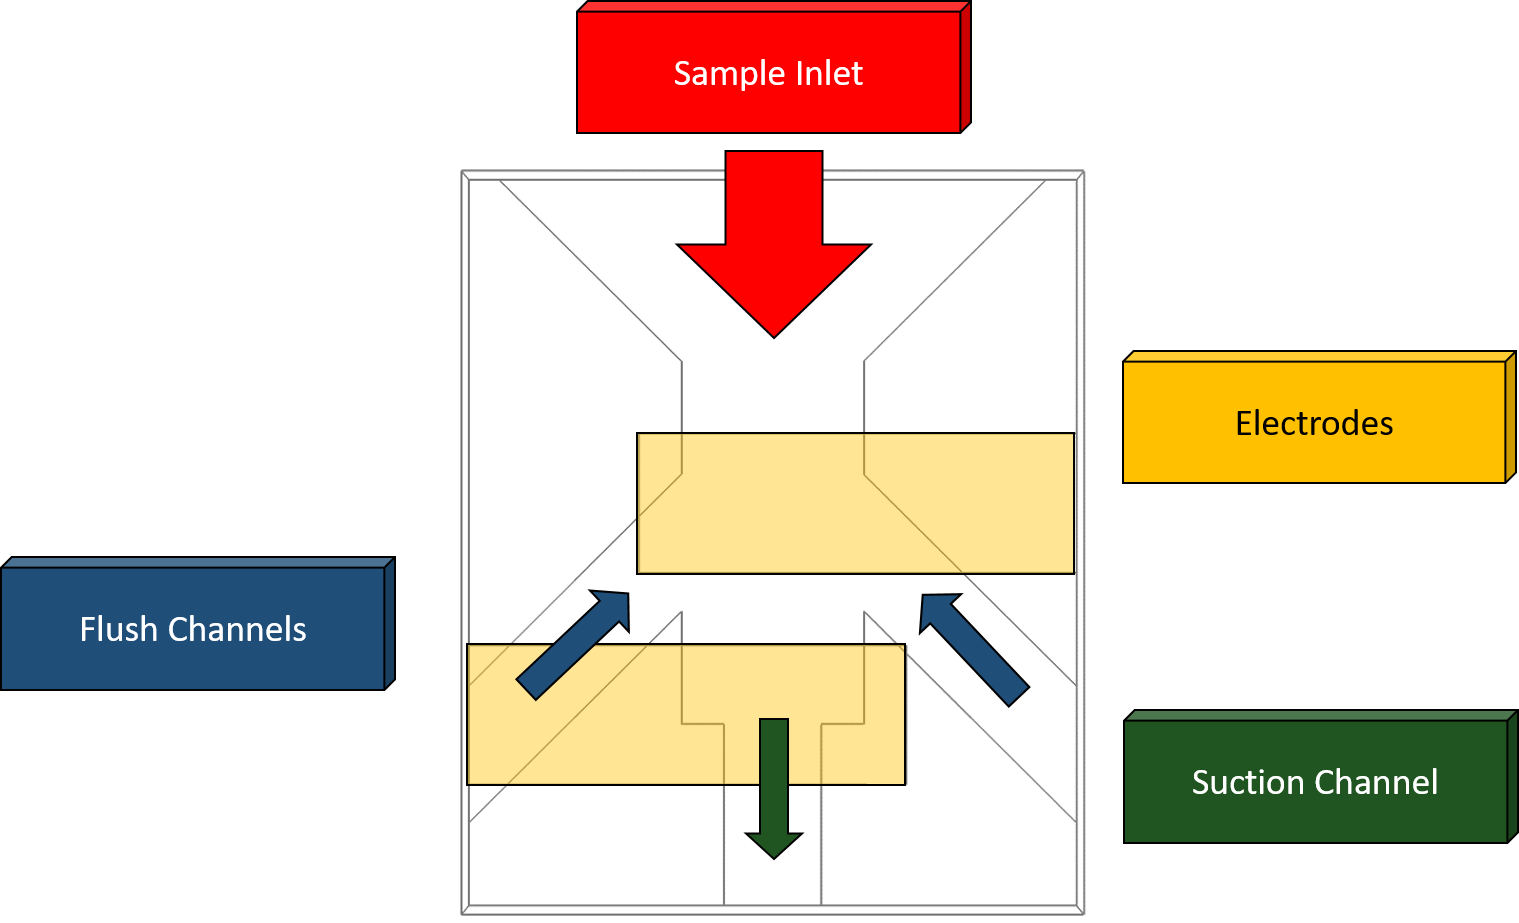
\includegraphics[width=\textwidth]{images/josh_steph_design.png}
    \caption{Functional diagram of cell impedance sensor chamber.}
    \label{fig:josh-steph_functional_diagram}
\end{figure}

\par The impedance sensor was designed with two 11.5 micron wide electrodes with a 5 micron gap that lays under a 15 by 15 micron target measurement area. The device isolates a cell by activating flush and suction channels once a cell from the sample inlet wanders into the test chamber with the purpose of keeping the cell in the test chamber and other cells out (figure \ref{fig:josh-steph_functional_diagram}). Once the device captures a cell, voltage signals over a range of frequencies are applied 

\begin{figure}[h]
    \centering
    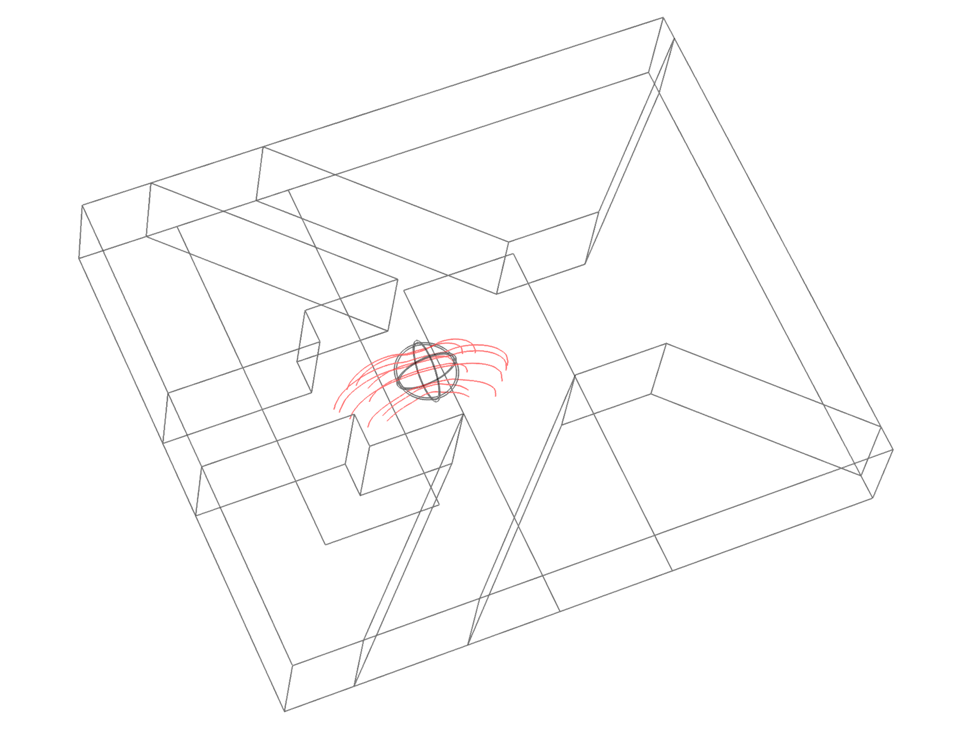
\includegraphics[width=0.9\textwidth]{images/josh_steph_sim.png}
    \caption{Example of desired device behaviour using a COMSOL simulation of electric field lines through a cell. A detailed description of the COMSOL model is presented in section \ref{}}
    \label{fig:josh-steph_sim}
\end{figure}


\begin{figure}[h]
    \centering
    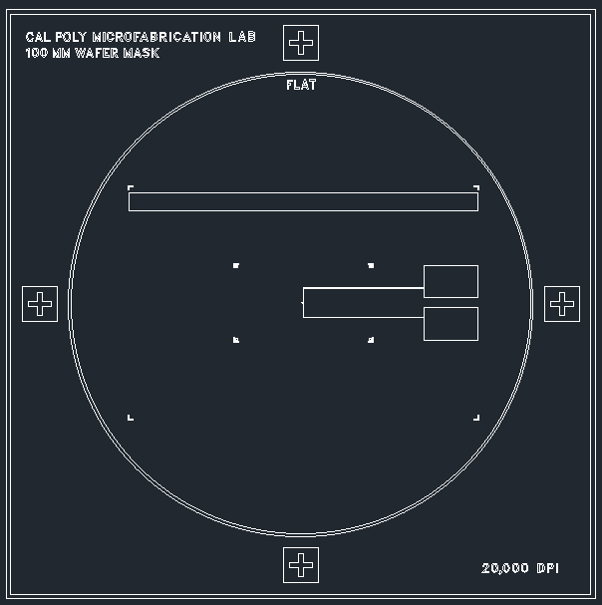
\includegraphics[width=0.6\textwidth]{images/electrode_mask.png}
    \caption{Electrode mask by Stephanie Hernandez \cite{hernandez_single_2009-1}}
    \label{fig:electrode_mask}
\end{figure}

\begin{figure}[h]
    \centering
    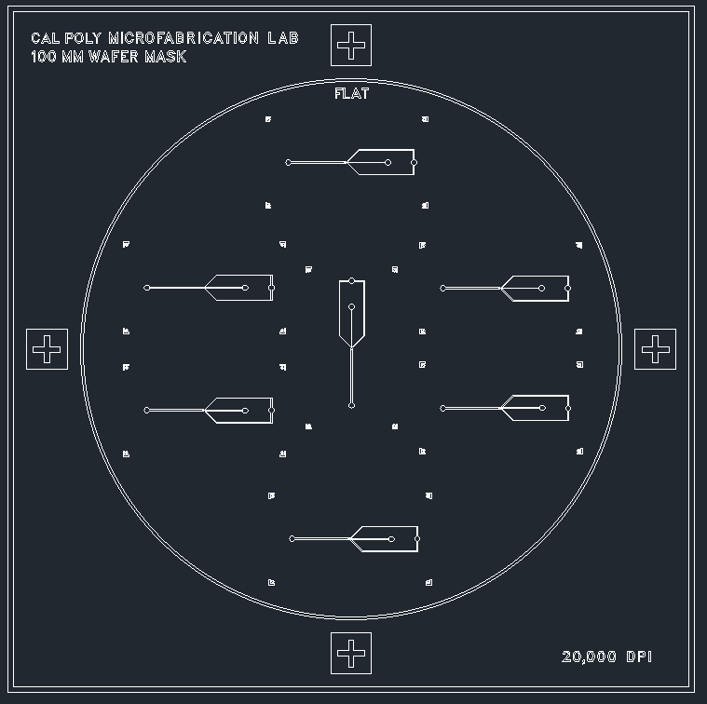
\includegraphics[width=0.6\textwidth]{images/micro_channel_mask.png}
    \caption{Micro channel mask by Josh Fadriquela \cite{fadriquela_design_2009-1}}
    \label{fig:microchannel_mask}
\end{figure}

\section[Objectives]{Thesis Purpose and Objectives}

%\chapter{Background}
%

%%%%%%%%%%%%%%%%%%%%%%%%%%%%%%%%%%
% Cells
%%%%%%%%%%%%%%%%%%%%%%%%%%%%%%%%%%
\section{Cells}
\par The cell is the basic unit of life. At the fundamental level, a cell must have an outer membrane that acts as a gatekeeper between the surrounding environment and the interior constituents. The contents of the cell interior varies widely between organisms, cell specializations, and states of each cell. For example, mature red blood cells do not contain a nuclei or any genetic material, but skeletal muscle fiber consist multiple nuclei \cite{daniel_d_chiras_human_2005}. However, all these variations can be generalized to useful cell models, such as the model for human cells in figure \ref{fig:human_cell_model}.   
\begin{figure}[ht]
 \centering
 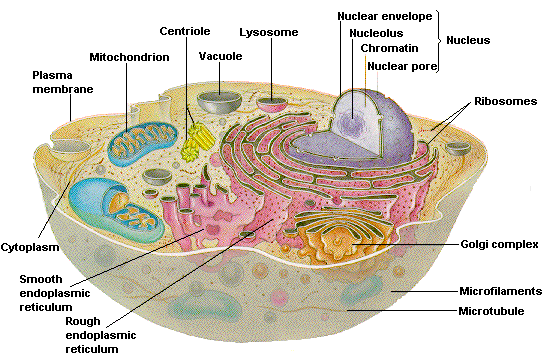
\includegraphics[width=\textwidth]{images/humanCellOverview.png}
 \caption[Diagram of human cell structure.]{Diagram of human cell structure. \cite{daniel_d_chiras_human_2005} }
 \label{fig:human_cell_model}
 \end{figure}
 
 \par Generally, a cell carries genetic information in the nucleus which is inside the cell membrane and cytoplasm. Cytoplasm is the cell material inside of the cell membrane and outside the nuclei. The cytoplasm consists of non-nuclei organelles and cytosol.  Cytosol refers to the cellular solution between the cell organelles and the membrane, wich contains salts, nucleic acids and cytoskeleton filaments \cite{daniel_d_chiras_human_2005}. Organnelles are membrane bound structures inside the cell that perform special functions. Organelles include nuclei, mitochondria, the Golgi apparatus, lysosomes, and vacuoles.  
 
 %%%%%%%%%%%%%%%%%%%%%%%%%%%%%
 % The Cell Membrane
 %%%%%%%%%%%%%%%%%%%%%%%%%%%%%
 \subsection{The Cell Membrane}
 \par The cell membrane is an essential component of the cell that is necessary for signalling, extracellular interaction, and maintaining equilibrium. The membrane is primarily composed of the lipid bilayer which is a semi-permeable barrier constructed from phospholipids. A phospholipid has a hydrophilic head group and a hydrophobic tail group. When exposed to an aqueous environment, phospholipids join together into a configuration that leaves the head groups exposed to the aqueous solution and the tail group surrounded by other non-polar tail groups. In the case of a cell, the phospholipids take the form of a spherical bilayer membrane (figure \ref{fig:cell_membrane}). The membrane forms a semi-permeable membrane that allows for restricted diffusion of certain molecules. 
 
 \par In addition to phospholipids, the cell membrane is packed with proteins that are critical for a range of functions. Of interest to this thesis, are channel and transport proteins that allow controlled passage of molecules through the membrane. 
 
 \begin{figure}[h]
    \centering
    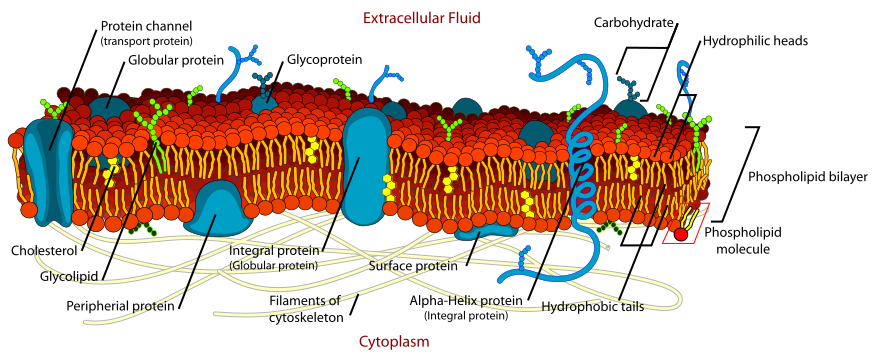
\includegraphics[width=\textwidth]{images/Cell_membrane_detailed_diagram.png}
    \caption[Diagram of the cell membrane]{Diagram of the cell membrane \cite{mariana_ruiz_cell_????}}
    \label{fig:cell_membrane}
 \end{figure}
 
 
 %%%%%%%%%%%%%%%%%%%%%%%%%%%%%%%%%%%%%%%%%
 % Electrical Model of the Cell
 %%%%%%%%%%%%%%%%%%%%%%%%%%%%%%%%%%%%%%%%%
\subsection{The Electrical Model of the Cell}

\par The state of a cell directly affects the cell electrical properties and measuring these properties provides insight into the cell state, type, and afflictions. A common model of the bulk electrical model of a cell is presented in figure \ref{fig:electric_model_cell}. As a bulk electrical element, the cell membrane can be modeled as a leaky capacitor that can accumulate a charge differential, but also leaks charges across the membrane. This behaviour can be modeled as a resistor and capacitor in parallel. The membrane capacitance is supplemented by the formation of an electric double layer (EDL). A biological cell carries a net negative charge which results in the development of a 10-100 nm thick electric double layer surrounding the cell in electrolyte solutions \cite{swaminathan_effect_2009}. The electric double layer contributes to the capacitance of the cell membrane. The EDL will be described in further detail in section \ref{sec:the_electric_double_layer}. The bulk electrical properties of the cytoplasm are often modeled as a RC series circuit with a relatively large capacitance. 

\begin{figure}
    \centering
    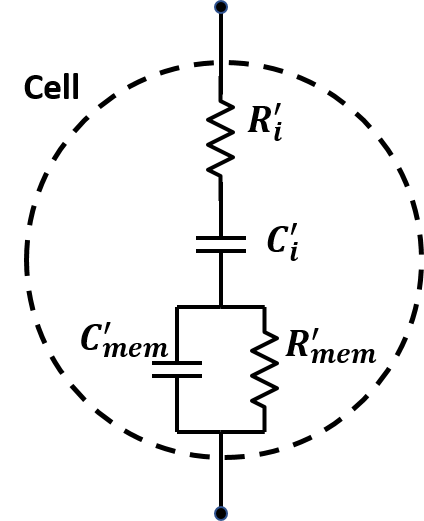
\includegraphics[width=0.4\textwidth]{images/completeCellCircuit.png}
    \caption[Electrical model of single shelled cell.]{Electrical model of single shelled cell. $R'_i$ and $C'_i$ are the resistance and capacitance of the cytoplasm, and $R'_{mem}$ and $C'_{mem}$ are the resistance and capacitance of the membrane}
    \label{fig:electric_model_cell}
\end{figure}
 
 %%%%%%%%%%%%%%%%%%%%%%%%%%%%%%%%
 % Dielectric Spectroscopy
 %%%%%%%%%%%%%%%%%%%%%%%%%%%%%%%%
 \section{Dielectric Spectroscopy}

 % Read into articles and provide more details
 
 \par The dielectric properties of cells have been investigated since 1910 when H\"{o}ber showed the existence of the cell membrane by measuring the conductivity of erythrocytes (red blood cells) at high and low frequencies \cite{hober_r_methode_1910}. The field of study further developed with Fricke's application of Maxwell's equations to measure the capacitance and thickness of the cell membrane from 1924 to 1925 \cite{james_clerk_maxwell_treatise_1892, fricke_h_mathematical_1924, fricke_h_electric_1924, fricke_h_electric_1931}. 
 
 \par Then in 1998, Cole used Maxwell's mixture equation to derive the complex impedance of a single shelled cell model and developed equations to describe the Cole-Cole plot \cite{cole_electric_1928}. And with Curtis, Cole made the first single cell measurements on a Nitella cell (a large bacteria cell that ranges from 20 to 60 mm in length) \cite{curtis_transverse_1937}. 
 
 \par From 1957-1968 Schwan used broadband electric impedance spectroscopy to identify $\alpha$, $\beta$, and $\gamma$ dispersions of a cell \cite{schwan_h_p_electrical_1957,schwan_h_p_electrical_1963,schwan_electrical_1994}. A dielectric dispersion is a frequency range with a large change in permittivity with respect to frequency. The permittivity of a material is the resistance to forming an electric field over a medium. In general the effects of a source charge can be described as the polarization of surrounding medium and the residual electric field over the resisting polarized medium. For a dielectric material, the electric field may be thought of as having two components: the electric displacement vector $\boldsymbol{D}$ that accounts for the electric field generated from separated free electrical charges, and the polarization $\boldsymbol{P}$ which accounts for the bound polarization charges in a dielectric material. The effect of $\boldsymbol{P}$ is to attenuate of the electric field. This relationship can be observed by rearranging the definition of electric displacement.
 \begin{equation}
     \boldsymbol{D} = \epsilon_o \boldsymbol{E} + \boldsymbol{P},
     \label{eqn:electric_displacement}
 \end{equation}
 \begin{equation}
    \boldsymbol{E} = \frac{1}{\epsilon_o}\Big(\boldsymbol{D} - \boldsymbol{P}\Big),
 \end{equation}
 
 \noindent where $\epsilon_o$ is known as the dielectric constant or the permittivity of the vacuum, with a value of 8.85E-12 F/m.
 
 \par For a linear dielectric medium, the polarization can be defined as 
 \begin{equation}
     \boldsymbol{P} = \epsilon_o\chi\boldsymbol{E},
     \label{eqn:polarization}
 \end{equation}
 \noindent where $\chi$ is the electric susceptibility. Substituting equation \ref{eqn:polarization} into \ref{eqn:electric_displacement}
 \begin{equation}
    \boldsymbol{D} = \epsilon_o(1+\chi)\boldsymbol{E} = \epsilon_o \epsilon_r \boldsymbol{E}=\epsilon\boldsymbol{E},
 \end{equation}
 
 \noindent where $\epsilon = \epsilon_o\epsilon_r$ is the permittivity and $\epsilon_r = 1 + \chi$ is the relative permittivity of a medium. For the case of isotropic materials, $\chi$ and $\epsilon$ reduce to scalar values, but for anisotropic materials, they are expressed as second order tensors. The susceptibility of a material describes how a material polarizes under an electric field and the permittivity describes the resistance to forming an electric field over that material. For dielectrics, the permittivity and susceptibility are closely related, but due to the resistance to forming an electric field over a vacuum, the two quantities are subtly different. The permittivity of a dielectric can be viewed as the sum of resistance to forming an electric field over a vacuum and the effect of polarizing a material.  Figure \ref{tab:permittivity_table} list the permittivity and susceptibility of some common materials.
 
 \begin{table}[h]
     \centering
     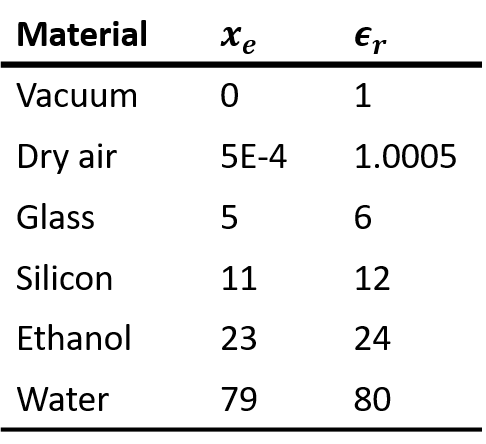
\includegraphics[width=0.4\textwidth]{images/permittivityTable.png}
     \caption[Permittivities of and susceptibilities of common materials]{Permittivities of and susceptibilities of common materials \cite{kirby_micro-and_2010}.}
     \label{tab:permittivity_table}
 \end{table}

 \par The frequency dependence of the permittivity arises from the time dependent material polarization or charge reorganization. Examples of charge reorganization include electron cloud distortion, charged particle displacement, and reorientation of molecules with dipoles. $\alpha$, $\beta$, and $\gamma$ dispersions refers to the ranges of alternating current frequencies where the permittivity decreases significantly in cells (i.e. dielectric relaxation). Figure \ref{fig:schwan_dispersions} depicts an approximate permittivity spectrum of a cell.
 
 \begin{figure}[ht]
 \centering
 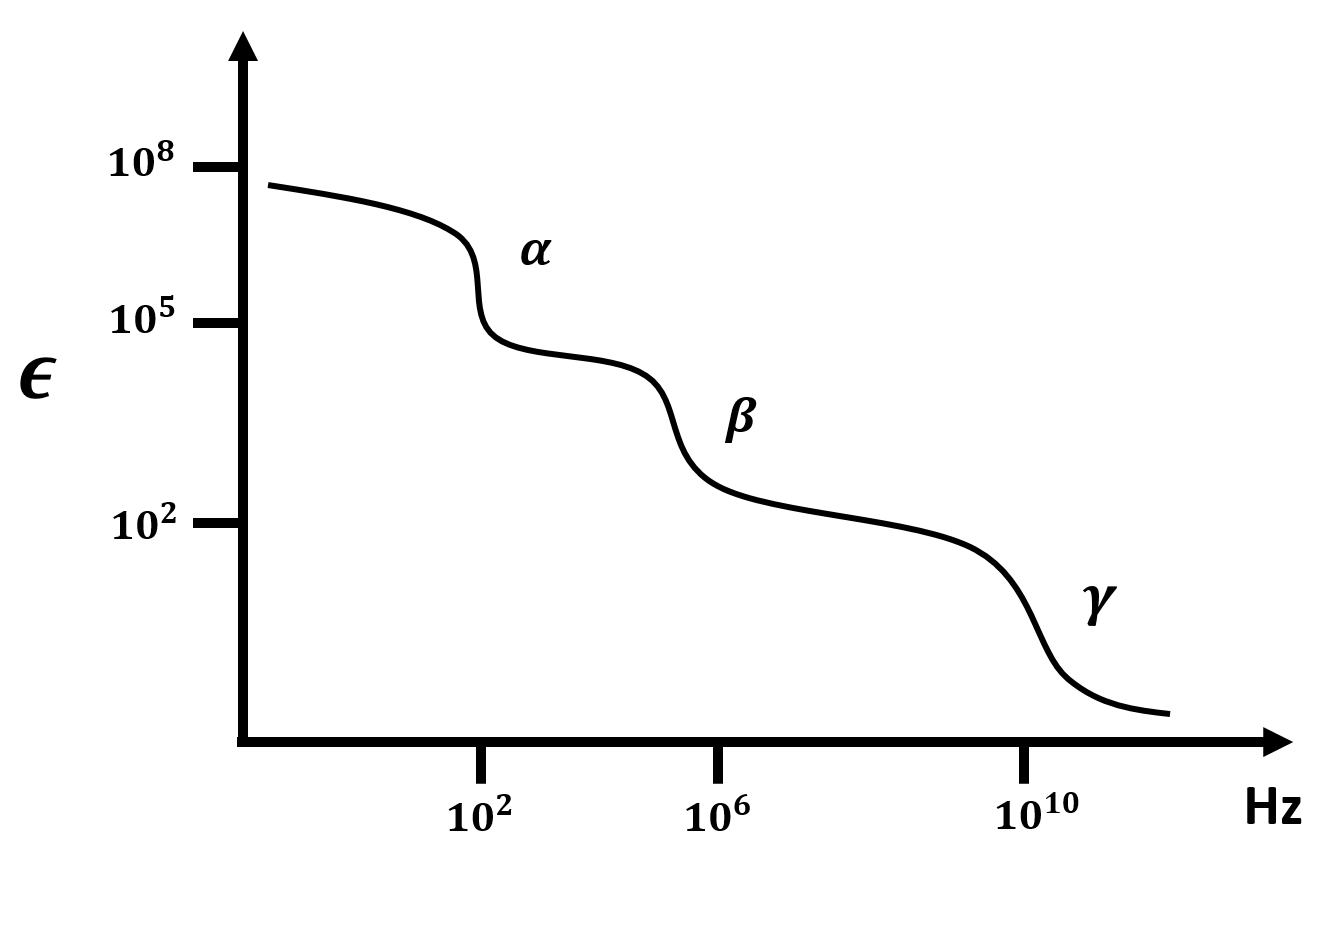
\includegraphics[width=0.7\textwidth]{images/schwanDispersions.png}
 \caption[General cell permittivity spectrum]{General cell permittivity spectrum with labeled $\alpha$, $\beta$ and $\gamma$ dispersions.}
 \label{fig:schwan_dispersions}
 \end{figure}
 
 \par $\beta$ dispersions occurs up to 10 Mhz and is caused by the relaxation of the cell membrane. For lower frequencies, the membrane has enough time to charge and provide resistance to the electric field, but at frequencies greater than about 10 Mhz, the membrane does not have sufficient time to fully charge and provides little resistance to the electric field. $\gamma$ dispersion is related to the relaxation of water molecules. Instead of a charging membrane, $\gamma$ dispersion is due to the dipole rotation of the of water molecules and the biomolecules that water is bound to. The source of $\alpha$ dispersion is undetermined, but current theories include the surface reactance of the electric double layer near the charged cell, the impedance of the sarcoplasmic recticulum (for muscle fibers), or the frequency dependent conductance of ionic membrane channels as predicted by the Hodgkin-Huxley equations \cite{schwan_electrical_1994}.
 
 
 \par These developments laid the foundations for the following techniques for measuring the dielectric properties of single cells. 
 
 %%%%%%%%%%%%%%%%%%%%%%%%%%%%%%%%
 % Dielectrophoresis
 %%%%%%%%%%%%%%%%%%%%%%%%%%%%%%%%
 \subsection{Dielectrophoresis}
 \par The dielectrophoretic force (DEP) is the force generated on a particle suspended in a solution by the interaction of an applied nonuniform electric field and an induced dipole moment developed through Maxwell-Wagner polarization (a build up of charges at dielectric boundaries). Peter Debye and Herbert A. Pohl were among the first to develop dielectrophoresis and demonstrated how particles could be moved with nonuniform electric fields \cite{muller_potential_2003}. With an applied AC electric field, the average DEP force on a spherical particle is expressed as \cite{morgan_single_2007, green_dielectrophoresis_1999}
 
 \begin{equation}
     \big< F_{DEP} \big> = \pi \epsilon_m R^3 \text{Re}[\tilde{f}_{CM}] \nabla |\textbf{E}|^2 
     \label{eqn:dep_force}
 \end{equation}
 
 \noindent with
 
 \begin{equation}
     \tilde{f}_{CM} = \frac{\tilde{\epsilon}_p - \tilde{\epsilon}_m}{\tilde{\epsilon}_p + 2\tilde{\epsilon}_m} 
     \label{eqn:fcm_background}
 \end{equation}
 
 \noindent where $\epsilon_m$ is the permittivity of the medium, $R$ is the radius of the particle, $\tilde{f}_{CM}$ is the Clausius-Mossotti factor for spherical particles,  $\tilde{\epsilon}_p$ is the complex permittivity of the particle, $\tilde{\epsilon}_m$ is the complex permittivity of the medium, and $\textbf{E}$ is the electric field. For most cases, the complex permittivity can be expressed as 
 \begin{equation}
     \tilde{\epsilon} = \epsilon - j\frac{\sigma}{\omega}
 \end{equation}
\noindent where $\epsilon$ is the permittivity, $j = \sqrt{-1}$, $\sigma$ is the conductivity, and $\omega$ is the angular frequency. 

\par From equation \ref{eqn:dep_force} and \ref{eqn:fcm_background}, it can be noted that, given a non-uniform electric field, the magnitude of the dielectrophoretic force depends on the size of the particle and the polarizability of the particle with respect to the medium (i.e Re$\big[\tilde{f}_{CM}\big]$), and the sign of the force only relates to the polarizability of the particle and medium (figure \ref{fig:freq_crossover}). It should be noted that, based on equation \ref{eqn:fcm_background}, the real part of Clausius-Mossotti factor is restricted to less than 1 and greater than -0.5. However, for non-spherical shapes, such as elongated ellipses, equation \ref{eqn:fcm_background} does not satisfy the Clausius-Mossotti factor which can reach values far greater than 1.  


\begin{figure}[ht]
 \centering
 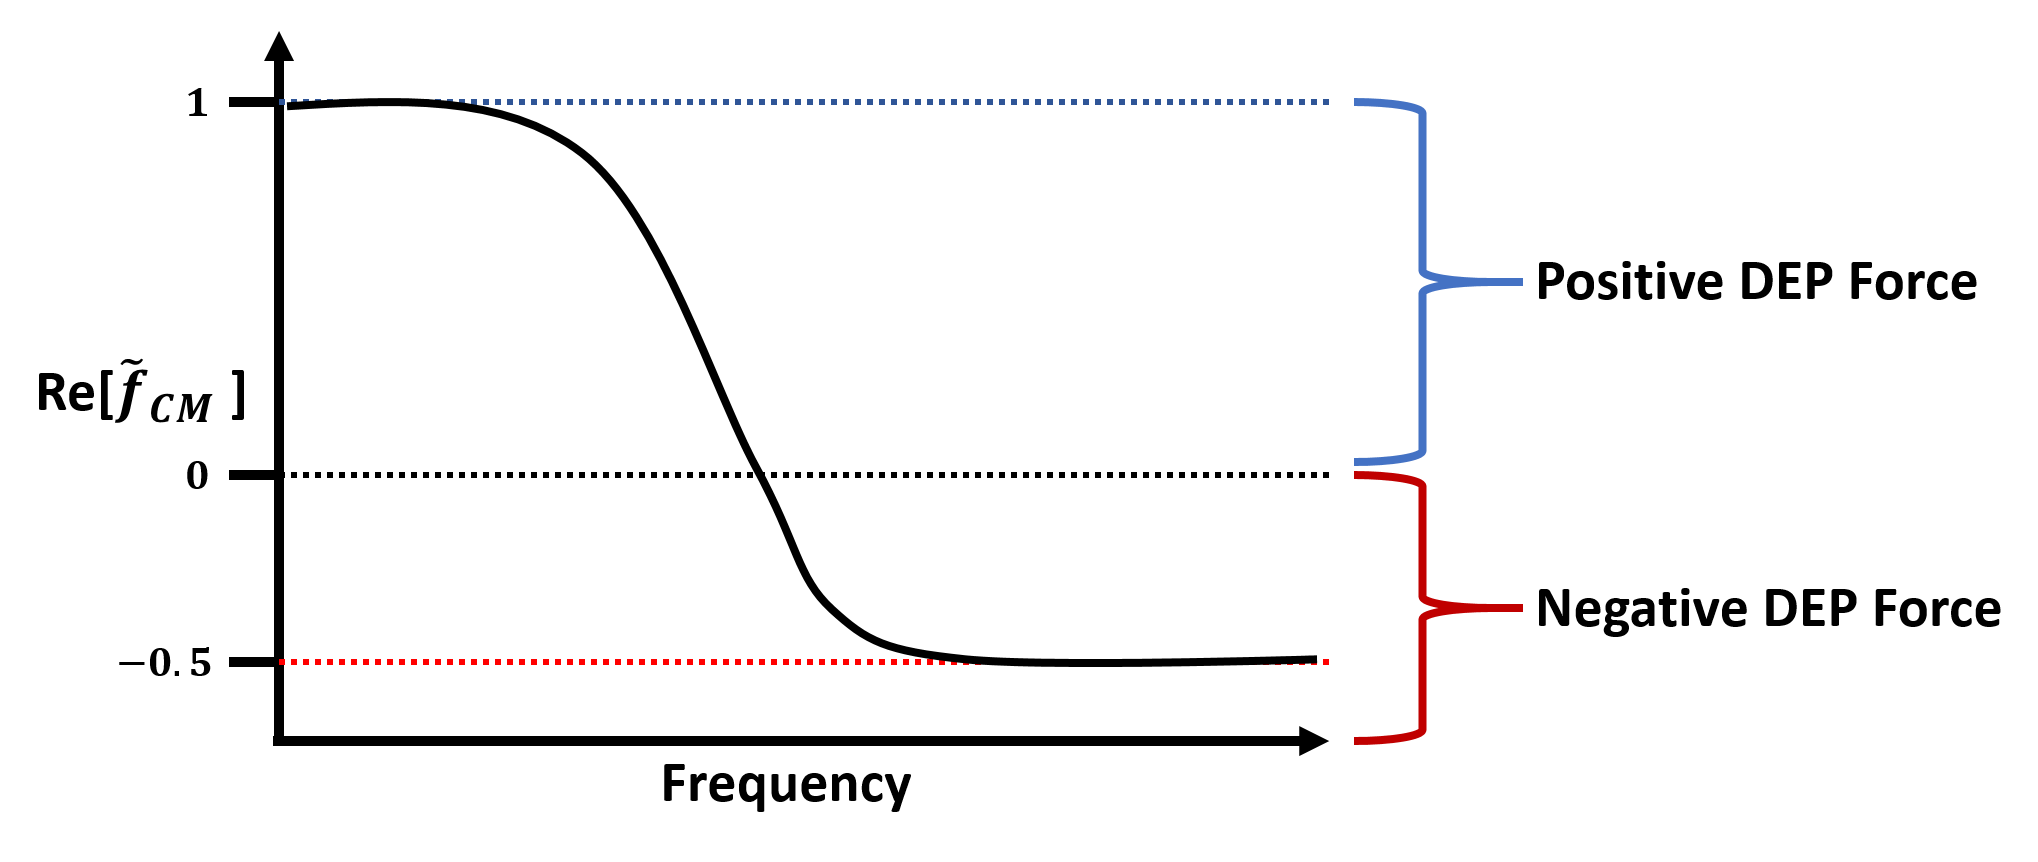
\includegraphics[width=\textwidth]{images/DEPCrossover.png}
 \caption[Frequency crossover of Clausius-Mossotti factor] {Frequency crossover of Clausius-Mossotti factor with labeled regions of positive and negative dielectriphoretic forces. From equation \ref{eqn:dep_force}, if $\tilde{\epsilon}_p$ is greater than $\tilde{\epsilon}_m$, then the DEP force is positive, if $\tilde{\epsilon}_m$ is less than $\tilde{\epsilon}_p$, then the DEP force is negative.}
 \label{fig:freq_crossover}
\end{figure}
 
 \par To extract dielectric properties of cells using dielectric forces, the DEP crossover frequency can be experimentally determined and compared to theoretical values \cite{morgan_single_2007}. The crossover frequency occurs at the frequency when the real part of the Clausius-Mossotti factor equals zero and is where the DEP force switches from a positive to a negative DEP force (or \textit{vice versa}). Experimentally, this can be determined by the observation of a stationary cell in a non-uniform electric field. Theoretically, the crossover frequency can be described as
 
 \begin{equation}
     f_{cross} = \frac{1}{2 \pi}\sqrt{\frac{(\sigma_m-\sigma_p)(\sigma_p+2\sigma_m)}{(\epsilon_p-\epsilon_m)(\epsilon_p+2\epsilon_m)}},
     \label{eqn:f_cross}
 \end{equation}
  
 \noindent where $f_{cross}$ is the crossover frequency, subscript $p$ denotes the particle, and subscript $m$ denotes the medium. Equation \ref{eqn:f_cross} can be rewritten to include the Maxwell-Wagner relaxation frequency as \cite{morgan_single_2007}
 
 \begin{equation}
    f_{cross} = \frac{1}{2 \pi} \sqrt{\frac{\sigma_m - \sigma_p}{\epsilon_p - \epsilon_m}f_{MW}},
 \end{equation}
 
 \noindent with
\begin{equation}
    f_{MW} = \frac{1}{2\pi\tau_{MW}},
\end{equation}
\begin{equation}
    \tau_{MW} = \frac{\epsilon_p + 2\epsilon_m}{\sigma_p + 2\sigma_m},
\end{equation}
 
 \noindent where $f_{MW}$ and $\tau_{MW}$ are the Maxwell-Wagner relaxation frequency and time constant respectively. The Maxwell-Wagner relaxation frequency characterizes the frequency of $\beta$ dispersion described by Schwan \cite{morgan_single_2007}.
 
 \par For a single shelled model of a cell, the crossover frequency can be expressed as
 \begin{equation}
     f_{cross} = \frac{\sqrt{2}}{8\pi R C_{mem}}\sqrt{(4\sigma_m - RG_{mem})^2 - 9R^2G^2_{mem}},
 \end{equation}
 
 \noindent where $C_{mem}$ is the specific capacitance of the cell membrane and $G_{mem}$ is the specific conductance of the membrane.
 
 %%%%%%%%%%%%%%%%%%%%%%%%%%%%
 % Electrorotation
 %%%%%%%%%%%%%%%%%%%%%%%%%%%%
 \subsection{Electrorotation}
 
 \par Electrorotation is the applied torque to a polarized particle in a medium of different dielectric properties by a rotating electric field. Such a field can be created with a system of four electrodes with sinusoidal signals of 90\textdegree \;phase shifts between adjacent electrodes \cite{goater_electrorotation_1999}. The phenomenon of electrorotation was first documented by Pohl in 1978 and then developed into dependable methods by Arnold and Zimmerman in 1982 \cite{pohl_dielectrophoresis_1978-1, arnold_rotating-field-induced_1982}.
 
 \par The average torque exerted on a spherical particle can be expressed as \cite{morgan_single_2007}
 \begin{equation}
    \Tau_{\text{ROT}} = -4\pi \epsilon_m R^3 \text{Im}\big[\tilde{f}_{CM}\big]|\textbf{E}|^2
    \label{eqn:ROT_torque}
 \end{equation}
 
 \noindent where $\Tau_{\text{ROT}}$ is the torque applied to the induced dipole of the particle, $\epsilon_m$ is the permittivity of the medium, $R$ is the radius of the spherical particle, $\textbf{E}$ is the electric field, and $\text{Im}\big[\tilde{f}_{CM}\big]$ is the imaginary part of the Clausius-Mossotti factor expressed in equation \ref{eqn:fcm_background}. Similar to the average dielectrophoretic force (equation \ref{eqn:dep_force}), the Clausius-Mossotti factor is the frequency dependent element and controls whether the particle rotates with or against the applied rotating electric field.
 
 \par The applied torque can be measured by the angular velocity of the particle, which can be expressed as \cite{morgan_ac_2003}
 \begin{equation}
     R_{\text{ROT}} = - \frac{\epsilon_m\text{Im}\big[\tilde{f}_{CM}\big]|\textbf{E}|^2}{2\eta}K, 
 \end{equation}
 \noindent where $R_{\text{ROT}}$ is the angular velocity, $\eta$ is the dynamic viscosity, and K is the scaling factor. When the angular velocity has reached equilibrium, the applied torque will be proportional $R_{\text{ROT}}$ and related by the scaling factor K. The electrorotation torque spectrum of a cell can be used, in tandem with equation \ref{eqn:ROT_torque}, to determine the dielectric properties of the cell. 
 
 \par By combining dielectrophoretic and electrorotaion spectroscopy techniques, significant details of the dielectric properties can be obtained. Since dielectrophoretic spectroscopy determines the real Clausius-Mossotti factor spectrum, and electrorotation determines the imaginary Clausius-Mossotti factor, the full $\tilde{f}_{CM}$ spectrum can deduced from which dielectric properties can be extracted. Separating the real and imaginary components of the Clausius-Mossotti factor, the following expressions are obtained \cite{hober_zweites_1912, morgan_single_2007}.
 \begin{equation}
     \text{Re}\big[\tilde{f}_{\text{CM}}\big] = \frac{(\sigma_p - \sigma_m)}{(1+\omega^2\tau_{\text{MW}}^2)(\sigma_p + 2\sigma_m)} + \frac{\omega^2\tau^2_{\text{MW}}(\epsilon_p-\epsilon_m)}{(1+\omega^2\tau_{\text{MW}}^2)(\epsilon_p+2\epsilon_m)}
 \end{equation}
 \begin{equation}
     \text{Im}\big[\tilde{f}_{\text{CM}} \big] = \frac{3\omega\tau_{\text{MW}}(\epsilon_p\sigma_m-\epsilon_m\sigma_p)}{(1+\omega^2\tau^2_{\text{MW}})(\epsilon_p+2\epsilon_m)(\sigma_p+2\sigma_m)}
 \end{equation}
 \par A major shortcoming of the previously discussed techniques is the long time needed for measurements. An electrorotaion assay could potentially take up to several seconds per test and limit the number of cells tested. An alternative approach, electric impedance spectroscopy, allows for rapid dielectric spectroscopy, and with flow-through designs, allows dielectric spectroscopy of every cell in a sample. 
 
 %%%%%%%%%%%%%%%%%%%%%%%%%%%%%%%%%%%%%%%%%%%%%
 % Electrical Impedance Spectroscopy
 %%%%%%%%%%%%%%%%%%%%%%%%%%%%%%%%%%%%%%%%%%%%%
 \subsection{Impedance Spectroscopy}
 \label{sec:impedance_spectroscopy}
 \subsection*{Impedance}
 \par Electrical Impedance is defined as the total opposition of a system to the flow of an alternating current (AC). If a sinusoidal voltage is applied to an arbitrary system, then the voltage and current can be expressed as
 \begin{equation}
    V(w) = |V|\cos(wt-\theta_V)
    \label{eqn:V(w)}
 \end{equation}
 \begin{equation}
    I(w) = |I|\cos(wt - \theta_I)
    \label{eqn:I(w)}
 \end{equation}
 \noindent where $w$ is the angular frequency, $t$ is the time in seconds, and $\theta_V$ and $\theta_I$ are the phase of $V$ and $I$ respectively. Using Euler's formula, equations \ref{eqn:V(w)} and \ref{eqn:I(w)} can be recognized as the real part of the following:
 \begin{equation}
    \hat{V}(w) = |V|e^{j(wt-\theta_V)}
 \end{equation}
 \begin{equation}
     \hat{I}(w) = |I|e^{j(wt-\theta_I)}
 \end{equation}
 
 \noindent Applying Ohm's law, the impedance of the system can be expressed as
 
 \begin{equation}
    Z = \frac{|V|}{|I|}e^{j(\theta_I-\theta_V)}
 \end{equation}
 \noindent or as 
 \begin{equation}
     Z = |Z|e^{j\theta}
     \label{eqn:impedance_euler}
 \end{equation}
 \noindent where $\theta$ is the difference in phase of the voltage from the current after the current passes through the system. Equation \ref{eqn:impedance_euler} sets the interpretation of impedance to be a vector that lives on the complex plane where $|Z|$ is the length of the vector, and $\theta$ is the angle of the vector from the positive real axis (figure \ref{fig:Impedance_diagram}).
 
 \begin{figure}[ht]
 \centering
 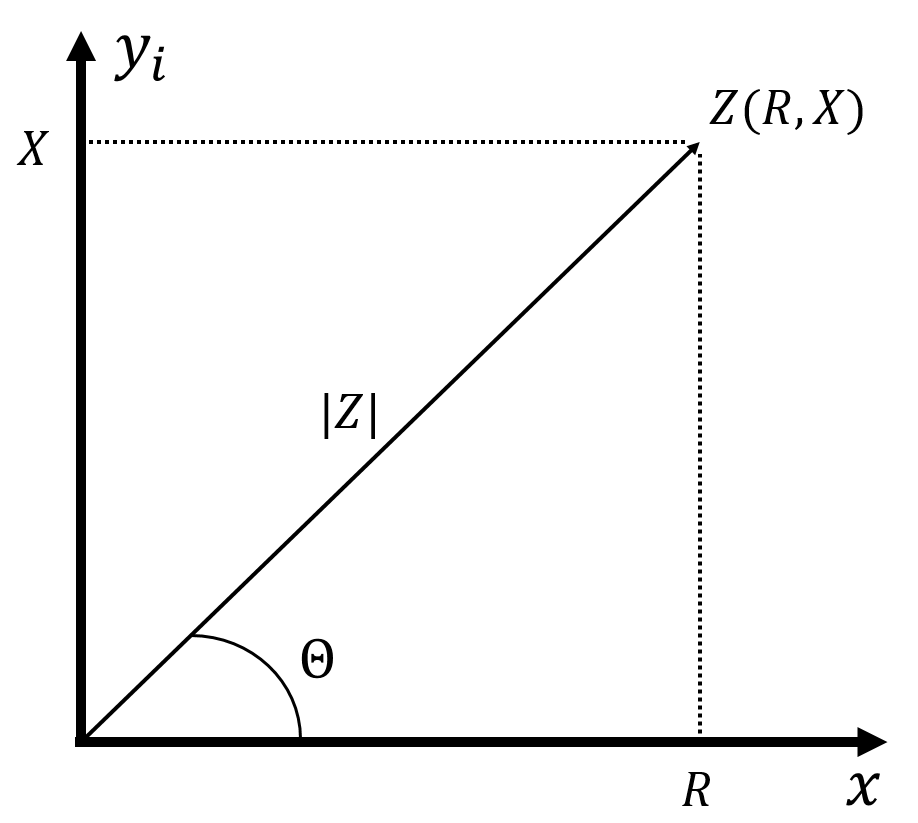
\includegraphics[width=0.7\textwidth]{images/impdedanceDiagram.png}
 \caption[Representation of impedance as a vector on the complex plane]{Representation of Impedance as a vector on the complex plane with a real component $R$ and imaginary component $X$. }
 \label{fig:Impedance_diagram}
 \end{figure}
 
 \par As a vector on the complex plane, impedance can be represented in rectangular coordinates and polar form:
 \begin{equation}
    Z = R + jX,
 \end{equation}
 \noindent where $R$ and $X$ are the real and imaginary components of the impedance vector, 
 \begin{equation}
     Z = |Z| \angle \theta
     \label{eqn:z_polar}
 \end{equation}
 \noindent where $|Z|$ is the magnitude of the impedance vector and $\theta$ is the angle of the vector from the positive real axis. Given an AC applied signal, Ohm's law can then be expressed as
 \begin{equation}
    |V| = |Z||I|,
    \label{eqn:ohm_mag}
 \end{equation}
 \noindent and the phase of the voltage signal will be shifted from the current signal by $\theta$. 
 
 \begin{figure}[ht]
    \centering
    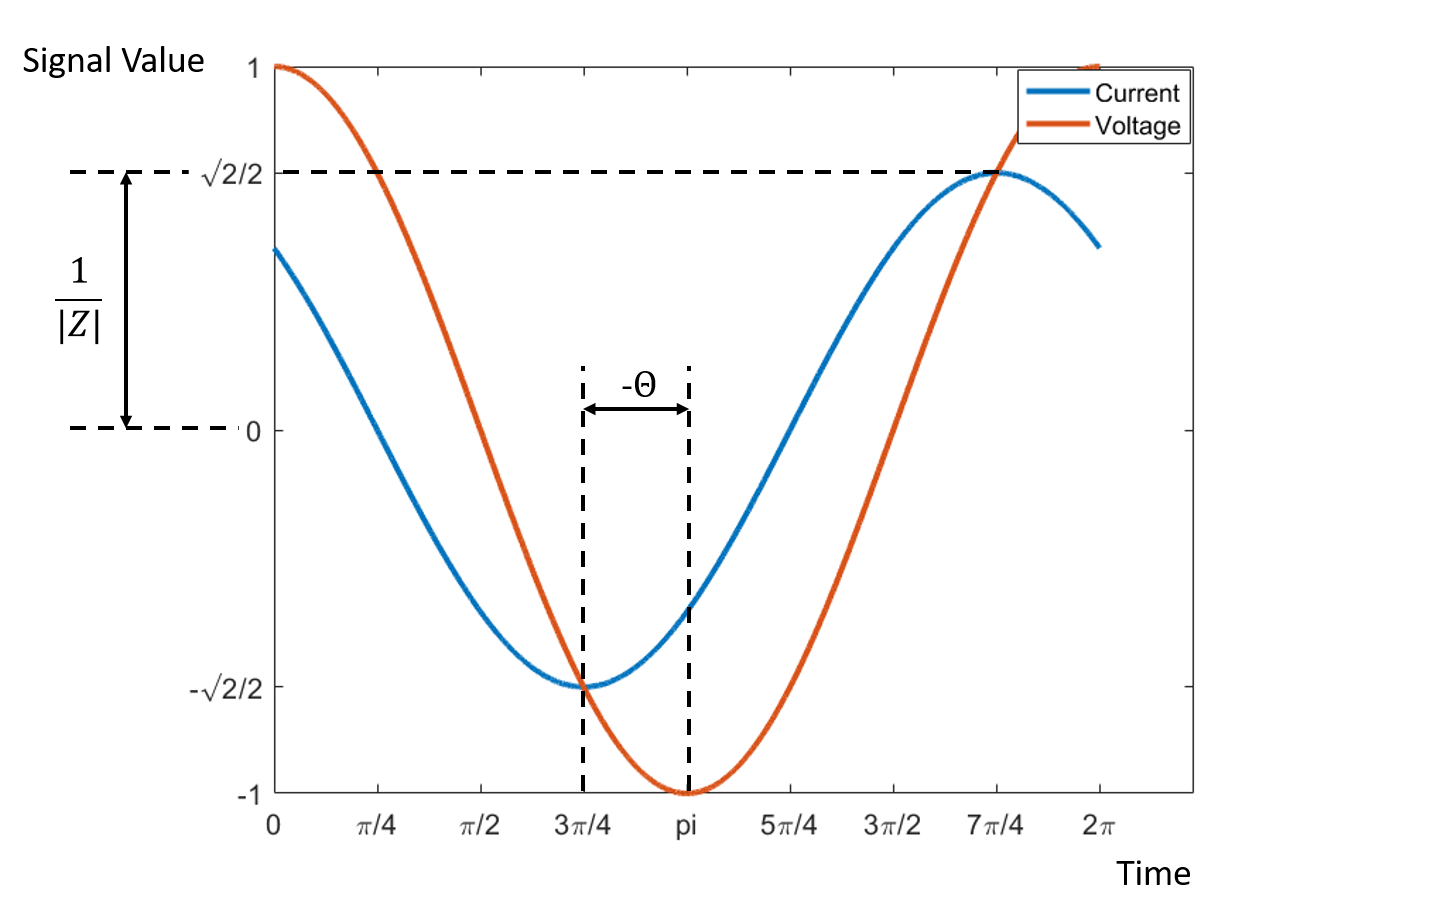
\includegraphics[width=0.9\textwidth]{images/ac_signal.png}
    \caption[Current Response of a system to an applied voltage]{Current Response of a system to a 1 volt applied potential. Using equations \ref{eqn:z_polar} and \ref{eqn:ohm_mag}, the impedance of the system can be expressed as $Z=\sqrt{2}\angle -\pi/4$} 
    \label{fig:ac_signal}
 \end{figure}
 
 \par The rectangular form and polar form of the impedance are related as follows:
 \begin{equation}
     |Z| = \sqrt{R^2 + X^2}
 \end{equation}
 \begin{equation}
    \theta = \text{arctan}\Big(\frac{X}{R}\Big)
 \end{equation}
 \begin{equation}
    R = |Z|\cos\theta
 \end{equation}
 \begin{equation}
     X = |Z|\sin\theta
 \end{equation}
 
 \par The impedance of a system can be represented by a combination of elementary circuit components: resistors, capacitors, and inductors. The voltage response of these elements in the time domain can be expressed as
 \begin{alignat}{2}
    &\text{Resistor:} \quad  &&V = IR \label{eqn:ohms_law}\\
    &\text{Capacitor:} \quad &&V = C \frac{dV}{dt}\\
    &\text{Inductor:} \quad  &&V = L \frac{dI}{dt}
 \end{alignat}
 \noindent where $V(t)$ and $I(t)$ are the voltage and current as a function of time, $R$ is the resistance, $C$ is the capacitance, $L$ is the inductance. After applying Laplace transforms, the frequency dependent impedance of each element can be obtained as
  \begin{alignat}{2}
    &\text{Resistor:} \quad  &&Z(w) = R \;\;\;\\
    &\text{Capacitor:} \quad &&Z(w) = \frac{1}{sC}\\
    &\text{Inductor:} \quad  &&Z(w) = sL
 \end{alignat}
 
 \noindent where $s=jw$ for steady state solutions.

\subsection*{Impedance Spectroscopy: Coulter Counter}
\par One of the first devices capable of measuring the electrical properties of particles is the Coulter counter, which measures the direct current resistance of two fluid filled chamber connected by an aperture (figure \ref{fig:coulter_counter}). The apparatus drives fluid through the aperture by a pressure differential caused by different levels of fluid in the two chambers. As particles flow through the aperture, conductive fluid is displaced and there is a change in resistance. Measuring the resistance over time, pulses of increased resistance marks a particle flowing through the aperture, and the magnitude of the resistance pulse will correspond to the size of the particle. 


\begin{figure}[ht]
    \centering
    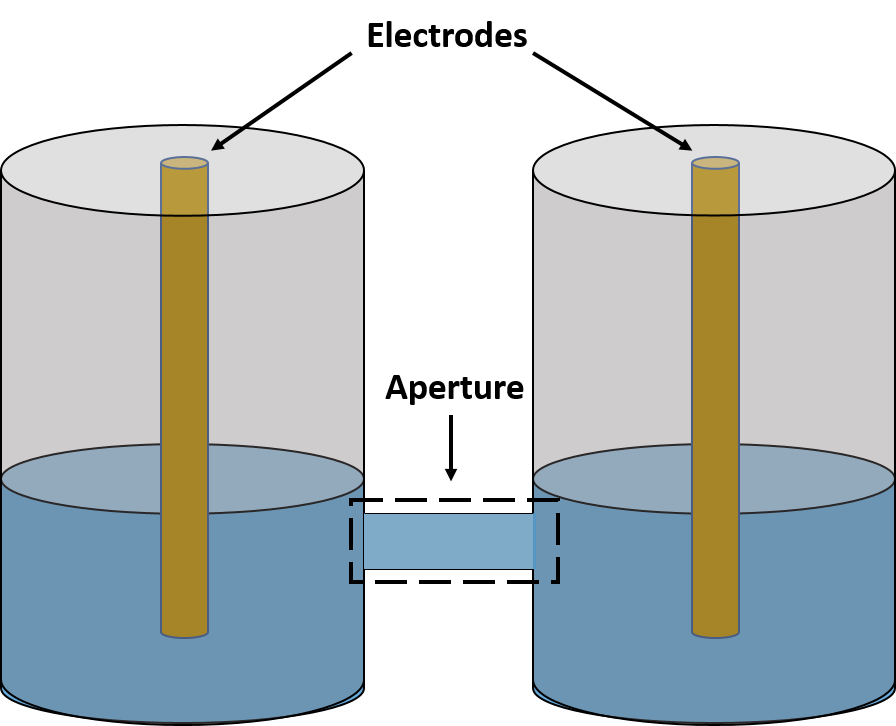
\includegraphics[width=0.8\textwidth]{images/coultierCounter.png}
    \caption[Illustration of Coulter counter principles]{A Coulter counter that measures the DC resistance of the fluid in the chamber with two electrodes. When a particle enters the aperture, the change in resistance will provide information about the size and electrical properties of the particle}
    \label{fig:coulter_counter}
\end{figure}


In 1970, Deblois and Bean developed an analytical model of the Coulter counter resistance that can be related to dielectric properties of the particle \cite{deblois_counting_1970}. The resistance of the large chambers were assumed to be negligible and the resistance of the aperture was derived (figure \ref{fig:aperture}). For a tube of a mixture solution, the resistance can be expressed as

\begin{equation}
    R_t = \frac{4\rho_{mix}L}{\pi d_{t}} G,
    \label{eqn:tube_resistance}
\end{equation}

\noindent where $G$ is a correction term for the non-uniform current density, $R_t$ is the resistance of the tube, $L$ is the length of the tube, $d_{t}$ is the diameter of the tube, and $\rho_{mix}$ is the resistivity of the mixture, which can be expressed using Maxwell's approximation, 

\begin{equation}
    \rho_{mix} = \rho_m\bigg[ 1 + \frac{3\phi}{2} + \Big(\frac{-9\phi \rho_m}{4 \rho_p + 2 \rho_m}\Big)\bigg],
\end{equation}
\noindent where $\phi$ is the volume fraction, $\rho_m$ is the resistivity of the conductivity, and $\rho_p$ is the resistivity of the particle. This approximation is only valid with the assumption that the particle diameter is small relative to the aperture. The volume fraction of a spherical particle in a tube is

\begin{equation}
    \phi = \frac{2d_p^3}{3d^2_tL}
\end{equation}

\noindent where $d_p$ is the diameter of the particle.

\begin{figure}[ht]
    \centering
    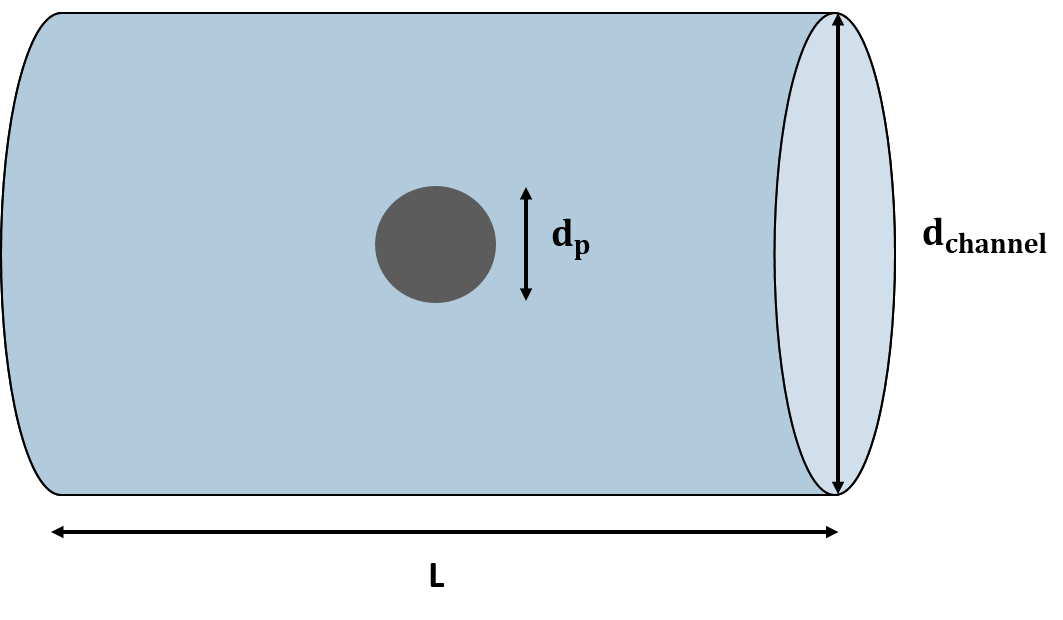
\includegraphics[width=0.7\textwidth]{images/aperture.png}
    \caption[The aperture connecting the two chamber of the Coulter counter.]{The aperture connecting the two chamber of the Coulter counter where $L$ is the length of the aperture, $d_p$ is the diameter of the particle flowing through the aperture, and $d_{t}$ is the diameter of the aperture.}
    \label{fig:aperture}
\end{figure}
 
\par Since 2000, Coulter counters have been fabricated on the micro scale and has allowed increased sensitivity and adaptability, leading to nanopore devices capable of analyzing single molecules \cite{sun_single-cell_2010}.
 
 \subsection*{Impedance Spectroscopy: Microfluidic Impedance Cytometry}
 \par Instead of electrodes on either side of an aperture, as in Coulter counter designs, microfluidic impedance cytometry designs electrodes directly onto the walls of the test volume. The test volume is the region that contains the particle and fluid with significant current density. The impedance of the test volume can be approximated as 
 \begin{equation}
       \tilde{Z}_{mix} = \frac{1}{jw\tilde{C}_{mix}}
    \label{eqn:impedance_with_cap}
 \end{equation}
 
 \noindent where $\tilde{C}_{mix}$ is the complex capacitance of the test volume, and can be expressed as
 \begin{equation}
     \tilde{C}_{mix} = \tilde{\epsilon}_{mix}G_f
 \end{equation}
 
 \noindent where $\tilde{\epsilon}_{mix}$ is the complex permittivity derived from Maxwell's mixture law and $G_f$ is the geometric factor that accounts for fringing electric fields. Further details are provided in section \ref{sec:theory_impedance_cytometry}.
 
 \begin{figure}[ht]
     \centering
     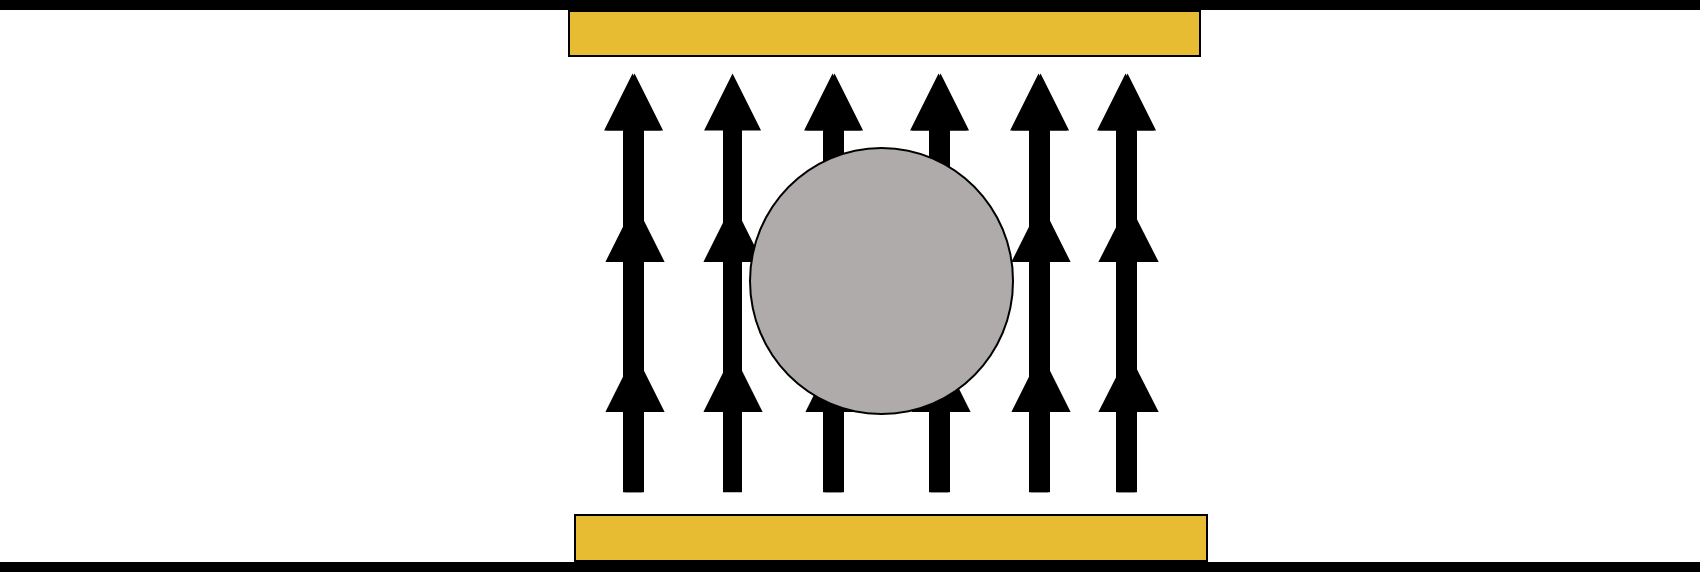
\includegraphics[width=\textwidth]{images/parallel.png}
     \caption{Parallel electrode configuration for impedance cytometry}
     \label{fig:parallel_electrodes}
 \end{figure}
 
 \par Common electrode configurations are parallel facing electrodes and coplanar electrodes (figure \ref{fig:parallel_electrodes} and \ref{fig:coplanar_electrodes}). Coplanar electrodes are easier to fabricate than parallel facing electrodes, but come at the cost of diminished sensitivity and accuracy \cite{sun_analytical_2007}. Parallel electrode systems produce smaller variations in the electric field compared to coplanar electrodes. As a result the signal variation be greater for coplanar configurations. This results in a loss of accuracy, unless the vertical placement of the cell in the test volume can be controlled. In addition, parallel facing electrodes designs generally have larger volume fractions, and therefore, are more sensitive than coplanar electrodes. This can be observed by noting that given an electrode width, channel height, and channel depth, the coplanar test volume will be over twice that of parallel electrodes configurations.
  
 
 \begin{figure}[ht]
     \centering
     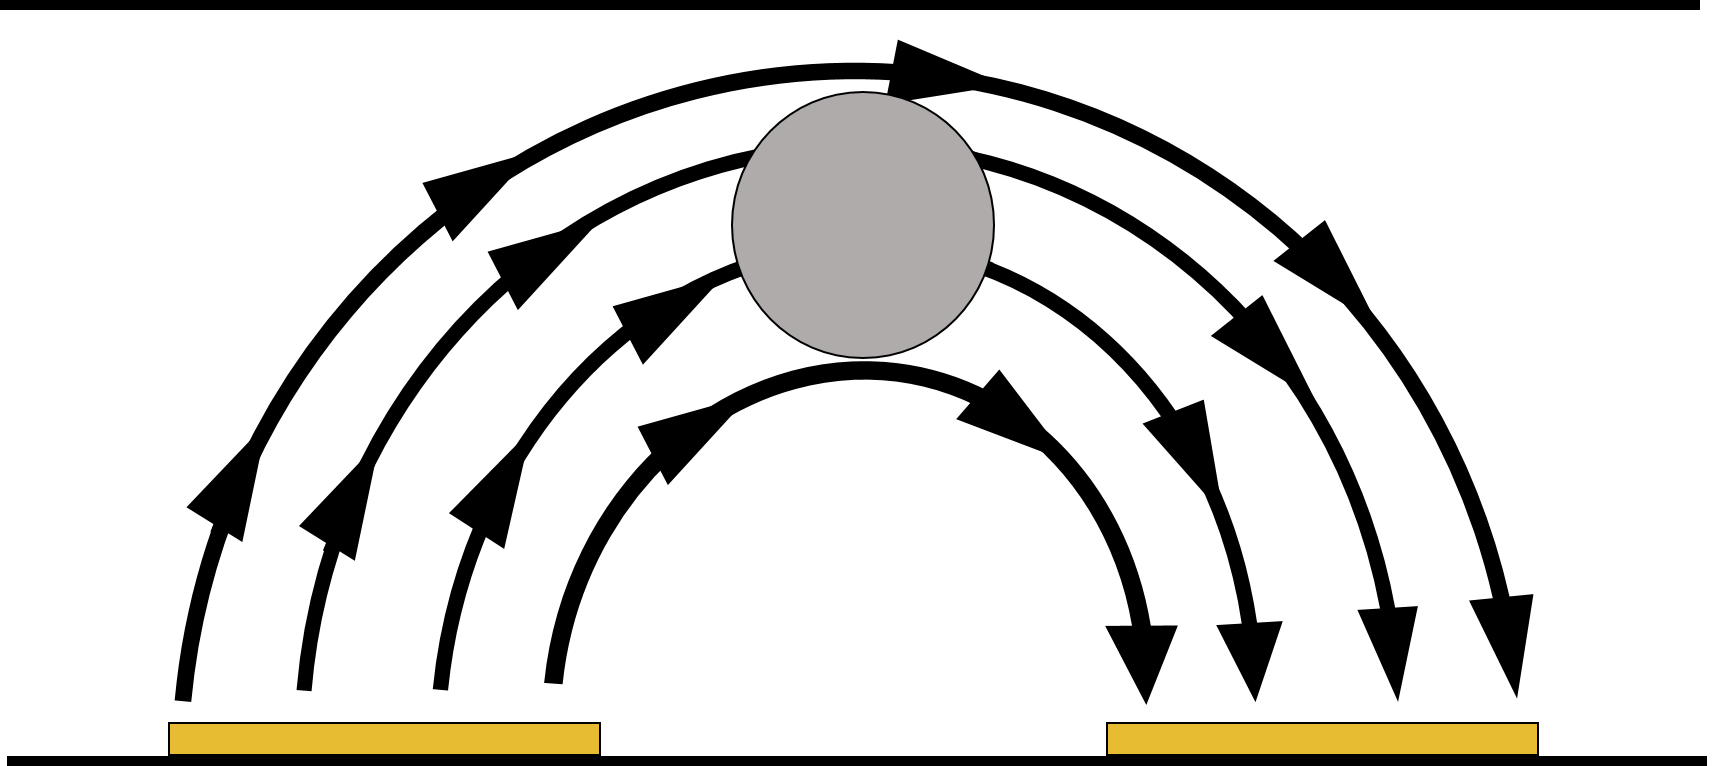
\includegraphics[width=\textwidth]{images/coplanar.png}
     \caption{Coplanar electrode configuration for impedance cytometry}
     \label{fig:coplanar_electrodes}
 \end{figure}
 
 \par In microfluidic impedance cytometry, alternating currents at a series of frequencies are applied to the system to see the impedance response over a range of frequencies. From this impedance spectrum, the frequency dependent complex response can be depicted as magnitude-phase plots, real-imamginary vs frequency plots, and nyquist plots in order to gain insight into the behaviour for the impedance response (figure \ref{fig:impedance_diagrams}). 
 

\begin{figure}[ht]
    \centering
    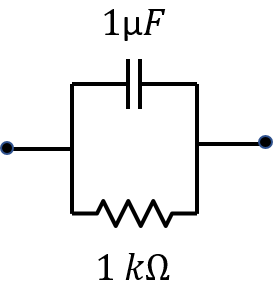
\includegraphics[width=0.3\textwidth]{images/exampleCircuit.png}
    \caption{Example circuit used in impedance diagrams}
    \label{fig:example_circuit}
\end{figure} 
 
 
 \begin{figure}
    \centering
    \begin{subfigure}[b]{\textwidth}
        \centering
        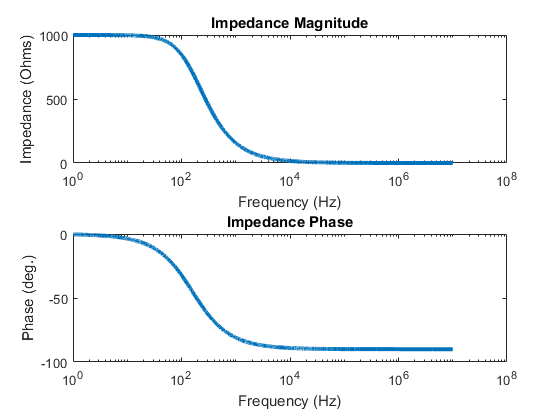
\includegraphics[width=0.68\textwidth]{images/magPhaseExample.png}
        \caption{Magnitude-phase versus frequency diagrams}
        \label{fig:mag_phase_ex}
    \end{subfigure}
 
    \begin{subfigure}[b]{\textwidth}
        \centering
        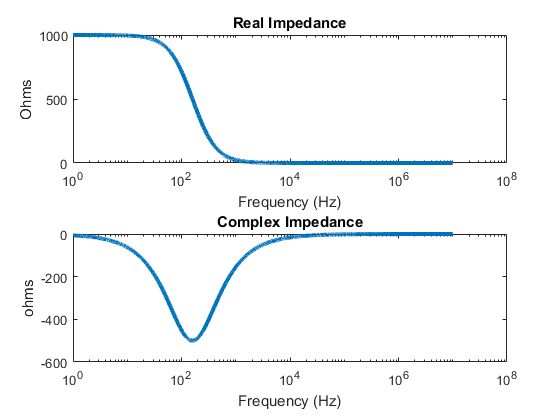
\includegraphics[width=0.68\textwidth]{images/complexRealExample.png}
        \caption{Real-imaginary versus frequency diagrams}
        \label{fig:real_complex_ex}
    \end{subfigure}
    \begin{subfigure}[b]{\textwidth}
        \centering
        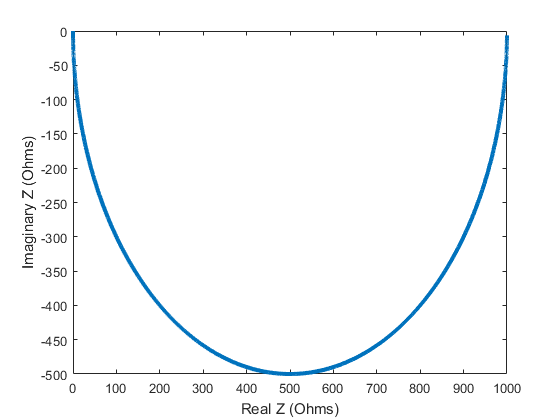
\includegraphics[width=0.52\textwidth]{images/nyquistExample.png}
        \caption{Nyquist plot}
        \label{fig:nyquist_plot}
    \end{subfigure}
    \caption[Impedance Diagrams]{Examples of magnitude-phase diagrams, real-complex diagrams, and a nyquist plot. The data is based off of the impedance of the circuit in figure \ref{fig:example_circuit}}
    \label{fig:impedance_diagrams}
\end{figure}

\par The 
 
 \subsection*{Circuit Implementation}
 \par The general process of impedance spectroscopy involves the application of a voltage or current signal, and the measurement of the signal response over a range of frequencies to obtain an impedance spectrum of the device under testing (DUT). The resulting spectrum provides insight into the dielectric properties of the DUT. 
 
 \par The simplest system for measuring impedance is the I-V method (figure \ref{fig:IV_impedance_measurement}). The I-V method determines the impedance of a DUT by measuring the voltage drop over the DUT and a high precision resistor in series. The current through the system can be calculated with Ohm's law at the high precision resistor. The impedance of the DUT for the I-V method can be expressed as 
 
 \begin{equation}
     Z_{DUT} = \frac{\Delta V_{DUT}}{I} = \frac{V_1 - V_2}{V_2}R
     \label{eqn:IV_Z}
 \end{equation}
 
 \noindent where $V_1$, $V_2$, and $R$ correspond to values of elements in figure \ref{fig:IV_impedance_measurement}. An important disadvantage of this configuration, is that the accuracy of the impedance values relies on the precision of the resistor value, the extent of the parasitic capacitance in the system, and quality of the probes measuring $V1$ and $V2$ which can be challenged under a large DUT impedance and high frequencies. If the I-V method is used, coaxial cables will result in inaccuracies.
 
 \begin{table}[ht]
    \centering
    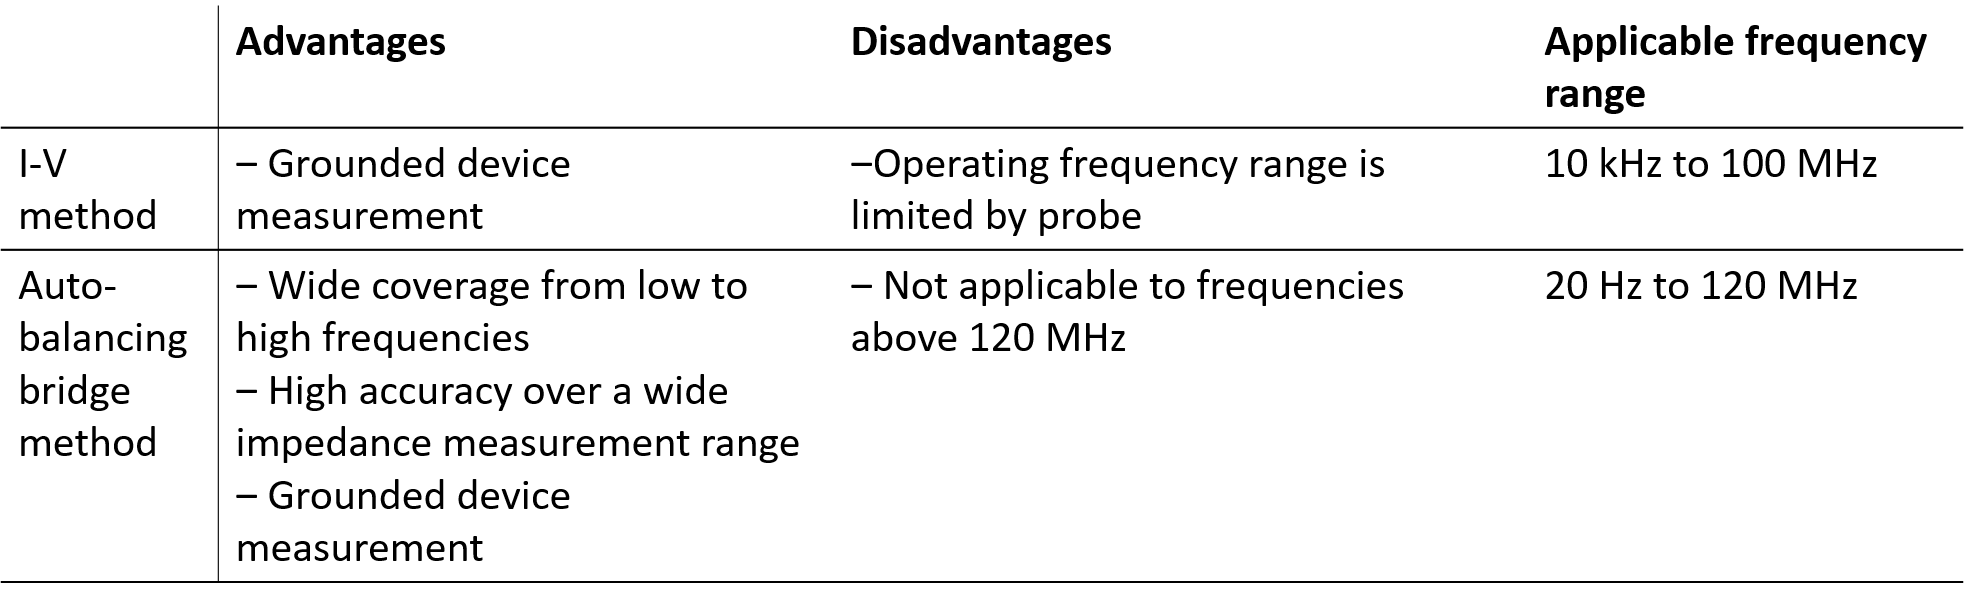
\includegraphics[width=\textwidth]{images/impedanceMeasurementMethods.png}
    \caption[Common impedance measurement methods]{Common impedance measurement methods \cite{keysight_technologies_impedance_2015}}
    \label{tab:z_measurement_methods}
 \end{table}
 
 \begin{figure}[ht]
    \centering
    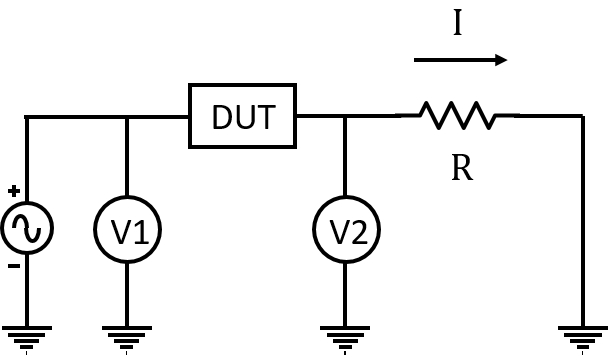
\includegraphics[width=0.7\textwidth]{images/I-VMethod.png}
    \caption[I-V impedance measurement configuration]{I-V impedance measurement }
    \label{fig:IV_impedance_measurement}
\end{figure}

\par Another circuit configuration to measure impedance is the auto-balancing bridge method (figure \ref{fig:auto-balancing_bridge}) \cite{keysight_technologies_impedance_2015}. The auto-balancing bridge method works as an extension of the I-V method. Instead of measuring the current directly, the potential on the low side of the DUT is driven to a virtual ground by an op-amp, and an equivalent current is measured. By applying Kirchoff's current law to virtual ground node, the impedance of the DUT for auto-balancing bridge can be expressed as

\begin{equation}
    \frac{V_1}{Z_{DUT}} - \frac{V_2}{R} = 0
\end{equation}
\begin{equation}
    Z_{DUT} = \frac{V_1}{V_2}R
\end{equation}

A significant advantage of the auto-balancing bridge method, is that when used with coaxial-grounded cables, the parasitic capacitance is removed from the measurement since all capacitances and measured elements are connected to ground. Although the distributed capacitance will affect the current drawn, it will not affect voltage readings and will significantly increase device accuracy.

 \begin{figure}[ht]
    \centering
    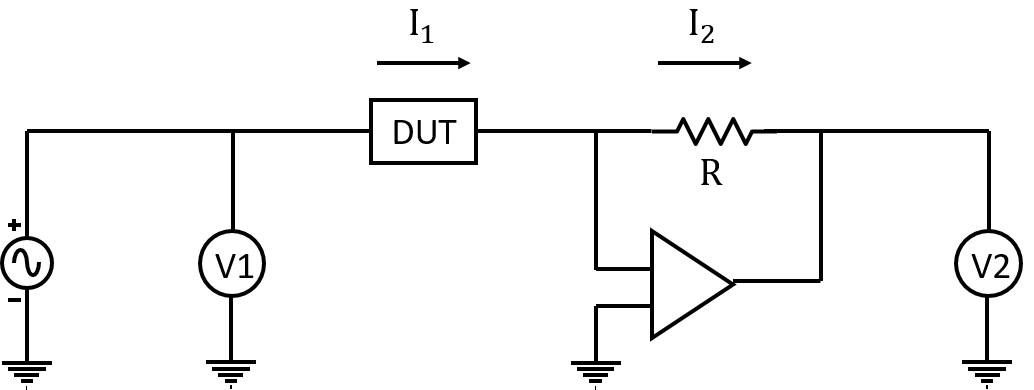
\includegraphics[width=\textwidth]{images/autoBalancingBridge.png}
    \caption[Auto-balancing bridge impedance method]{Auto-balancing bridge impedance method}
    \label{fig:auto-balancing_bridge}
\end{figure}
 
 % Electrical impedance spectroscopy has historically only been used on multiple cells to obtain aggregate data, however, with the rise of microelectomechanical systems (MEMS) and microfluidics, electrical impedance spectroscopy can be applied to individualy cells.
 
 %%%%%%%%%%%%%%%%%%%%%%%%%%%%%%%%%%%%
 % Theoretical Model of Impedance
 %%%%%%%%%%%%%%%%%%%%%%%%%%%%%%%%%%%%
 \section[Model of Cell Suspension Impedance]{Theoretical Model of Impedance Cytometry}
 \label{sec:theory_impedance_cytometry}

%%%%%%%%%%%%%%%%%%%%%%%%%%%%%%%%%%%%%
% Maxwell's Mixture Theory
%%%%%%%%%%%%%%%%%%%%%%%%%%%%%%%%%%%%%
\subsection{Maxwell's Mixture Theory}
 \begin{figure}[ht]
 \centering
 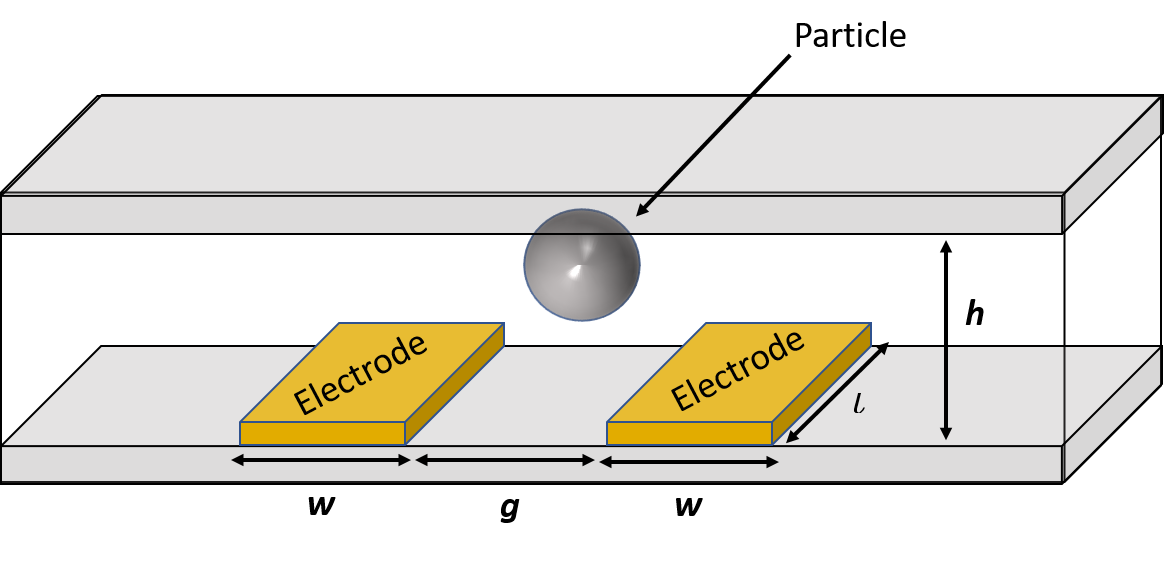
\includegraphics[width=0.7\textwidth]{images/cellAndElectrodes.png}
 \caption[Schematic diagram of simplified impedance sensor chamber.]{Schematic diagram of simplified impedance sensor chamber where w, $g$, and $l$ are the width, gap, and length of the electrodes respectively, and $h$ is the height of the chamber.}
 \label{fig:simplified_IS}
 \end{figure}
 
  \par The impedance of a single cell suspension, such as depicted in figure \ref{fig:simplified_IS}, can be solved for with Maxwell's mixture thoery \cite{james_clerk_maxwell_treatise_1892, sun_single-cell_2010}. Maxwell's equation for the complex permittivity of a mixture is
  \begin{equation}
      \tilde{\epsilon}_{mix} = \tilde{\epsilon}_m\frac{1 + 2\Phi\tilde{f}_{CM}}{1-\Phi\tilde{f}_{CM}},
  \end{equation}
  
  \noindent where $\tilde{\epsilon}_{mix}$ and $\tilde{\epsilon}_m$ are the complex permittivity of the mixture and medium respectively, $\tilde{f}_{CM}$ is the Clausius Mossotti factor, and $\Phi$ is the volume fraction. For most cases, the complex permittivity can be expressed as
  \begin{equation}
    \tilde{\epsilon} = \epsilon - j\frac{\sigma}{\omega},
\end{equation}

\noindent where $\epsilon$ is the permittivity, $j = \sqrt{-1}$, $\sigma$ is the conductivity, and $\omega$ is the angular frequency. The Clausius Mossotti factor is defined as
  \begin{equation}
    \tilde{f}_{CM} = \frac{\tilde{\epsilon}_p - \tilde{\epsilon}_m}{\tilde{\epsilon}_p + 2\tilde{\epsilon}_m}, 
  \end{equation}
  
  \noindent where $\tilde{\epsilon}_p$ is the complex permittivity of the particle.

 \begin{figure}[ht]
 \centering
 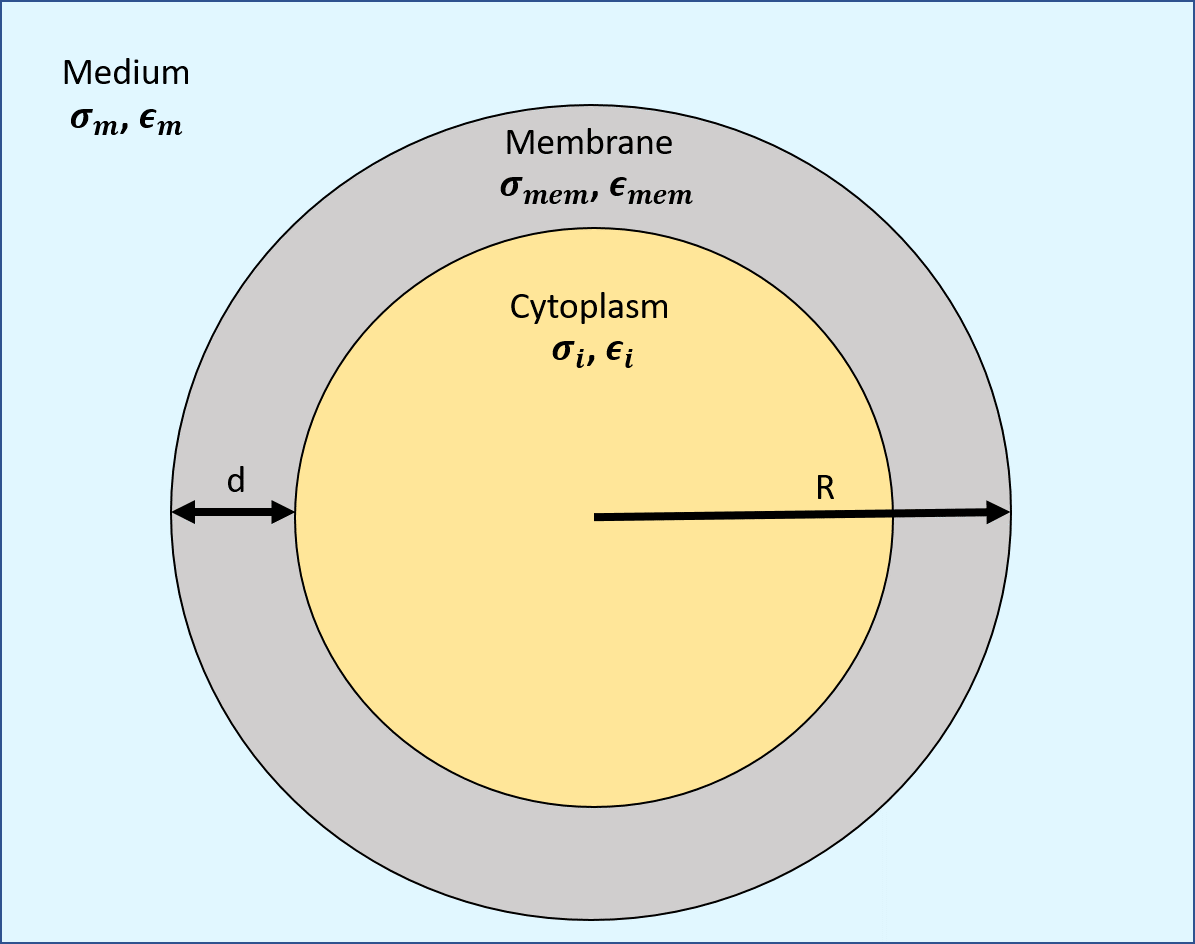
\includegraphics[width=0.7\textwidth]{images/singleShelledCell.png}
 \caption[Diagram of single shelled cell model.]{A diagram of a single shelled cell model where $\sigma$ is the conductivity, $\epsilon$ is the permittivity, and the subscripts $m$ and $i$ denote the membrane and cytoplasm respectively. $R$ and $d$ are the radius of the cell and membrane thickness respectively.}
 \label{fig:single_shell}
 \end{figure}

  \par The permittivity of the single shelled cell in figure \ref{fig:single_shell}, can be modelled as
  \begin{equation}
      \tilde{\epsilon}_p = \tilde{\epsilon}_{mem} 
      \frac{\gamma^3+2(\frac{\tilde{\epsilon}_i - \tilde{\epsilon}_{mem}}
      {\tilde{\epsilon}_i + 2\tilde{\epsilon}_{mem}})}{\gamma^3 - (\frac{\tilde{\epsilon}_i - \tilde{\epsilon}_{mem}}{\tilde{\epsilon}_i + 2\tilde{\epsilon}_{mem}})} \;\;\text{  with } 
      \gamma = \frac{R + d}{R}, 
  \end{equation}
  
  \noindent where $\tilde{\epsilon}_i$ is the complex permittivity of the cytoplasm, $\tilde{\epsilon}_{mem}$ is the complex permittivity of the cell membrane, $R$ is the radius of the cell, and $d$ is the thickness of the cell membrane.
  
  \par A corrected volume fraction is used to compensate for the fringe fields of the non-uniform electric field produced by the electrodes in figure \ref{fig:simplified_IS} \cite{gawad_micromachined_2001}. 
  
  \begin{equation}
      \Phi = \frac{4}{3} \pi R^3 \frac{1}{G_f\text{w}h},
      \label{eqn:corrected_vf}
  \end{equation}
  
  \noindent where $h$ is the height of the channel, w is the width of the electrode and $G_f$ is a geometric factor dependent on the geometry of the channel and electrodes.
  
  \par The impedance of the mixture is
  \begin{equation}
    \tilde{Z}_{mix} = \frac{1}{jw\tilde{C}_{mix}},
    \label{eqn:impedance_with_cap}
  \end{equation}
  
  \noindent where $w$ is the angular frequency and $\tilde{C}_{mix}$ is the complex capacitance of the mixture and can be expressed as
  \begin{equation}
      \tilde{C}_{mix} = \tilde{\epsilon}_{mix} G_f.
      \label{eqn:capacitance_mix}
  \end{equation}
  
  \noindent If equations \ref{eqn:impedance_with_cap} and \ref{eqn:capacitance_mix} are combined, we obtain
  \begin{equation}
    \tilde{Z}_{mix} = \frac{1}{jw\tilde{\epsilon}_{mix}G_f}.
    \label{eqn:impedance_with_Gf}
  \end{equation}
  
  \par To find the value of the geometric factor $G_f$, the cell constant of electrodes must be determined.
  
  
  %%%%%%%%%%%%%%%%%%%%%%%%%%%%%%%%%%%
  % Electrode Cell Constant
  %%%%%%%%%%%%%%%%%%%%%%%%%%%%%%%%%%%
  \subsection{Electrode Cell Constant}
  
  \par The cell constant $\kappa$ is defined as the proportionality factor between the measured resistance $R_b$ and the resistivity $\rho$ of a material.
  \begin{equation}
      R_b = \kappa \rho
      \label{eqn:cell_constant_proportionality}
  \end{equation}
  
  \noindent  Olthius related the measured resistance to capacitance in order to derive an analytic solution to cell constant \cite{olthuis_theoretical_1995}. 
  
  \par To find $R_b$ for two electrodes with an interspatial material, the measured resistance can be related to capacitance via Ohm's law and Maxwell's equation.
  \begin{equation}
      RC = \frac{\oiint \epsilon \boldsymbol{E} \cdot d\boldsymbol{S}}{\oiint \sigma\boldsymbol{E}\cdot d\boldsymbol{S}}
      \label{eqn:RC_integral}
  \end{equation}
  
  \noindent where $R$ and $C$ are the resistance and capacitance between the electrodes, $\epsilon$ is the product of the relative and vacuum permittivity, $\boldsymbol{E}$ is the electric field vector, and the integral is taken over a surface including one electrode.
  
  \par If the interspatial material is homogeneous and isotropic, then equation \ref{eqn:RC_integral} can be reduced to
  \begin{equation}
      RC = \frac{\epsilon}{\sigma}
      \label{eqn:RC}
  \end{equation}
  
  \par If we take $R_b = R$, we can combine equation \ref{eqn:RC} and \ref{eqn:cell_constant_proportionality} to express the cell constant in terms of capacitance.
  \begin{equation}
      \kappa = \frac{\epsilon}{C}
      \label{eqn:cell_constant_C}
  \end{equation}
  
   \begin{figure}[ht]
  \centering
  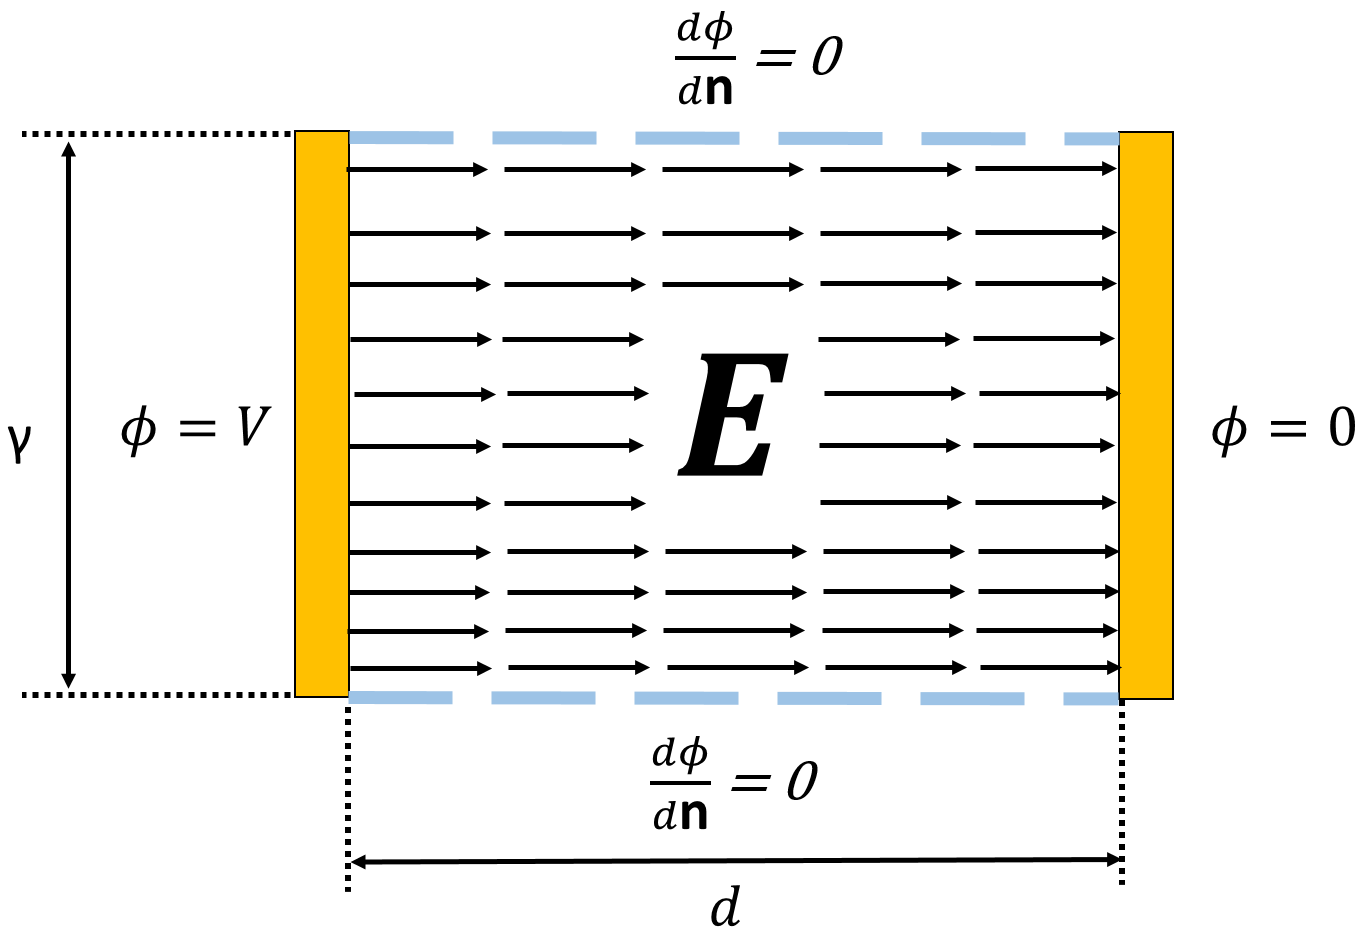
\includegraphics[width=0.7\textwidth]{images/capacitorNoFringe.png}
  \caption[Uniform electric field between parallel plates]{Uniform electric field between two parallel electrodes where $\boldsymbol{E}$ is the electric field, $\phi$ is the voltage, and $\frac{d\phi}{d\boldsymbol{n}}=0$ is the boundary condition of a perfect insulator. The dimensions of the capacitor are the electrode height $\gamma$, and the distance between the electrodes $d$.}
  \label{fig:parallel_capacitor}
  \end{figure}
  
  \par The capacitance of the two parallel plates with a uniform electrode field in figure \ref{fig:parallel_capacitor} is
  \begin{equation}
      C = \frac{\epsilon A}{d}
      \label{eqn:capacitor}
  \end{equation}
  
  \noindent where $A$ the area of the plate, and $d$ is the distance between the plates. Since $A = l\gamma$, where $l$ is the width, and $\gamma$ is the height of the electrode, the capacitance per unit width can be written as
  \begin{equation}
      C_l = \frac{\epsilon\gamma}{d} \;\;\;\text{where} \;\; C =l\, C_l
      \label{eqn:specific_capacitance}
  \end{equation}
  
  \par Returning to equation \ref{eqn:cell_constant_C}, and substituting equation \ref{eqn:specific_capacitance}, the cell constant can be expressed as 
  \begin{equation}
      \kappa = \frac{d}{\gamma \, l}
      \label{eqn:cell_constant}
  \end{equation}
  
  \noindent The geometric factor is related to the cell constant by 
  \begin{equation}
       G_f = \kappa \,l
       \label{geometric_cell}
  \end{equation}

  \noindent By combining equations \ref{eqn:cell_constant} and \ref{geometric_cell}, the geometric factor can be expressed as
  \begin{equation}
      G_f = \frac{d}{\gamma}
      \label{eqn:geometric_constant}
  \end{equation}
  
  \par Equation \ref{eqn:geometric_constant} is the solution of the geometric constant for the electrode configuration in figure \ref{fig:parallel_capacitor}, but to find the geometric constant for any other configuration, including the coplanar electrode in figure \ref{fig:simplified_IS}, $d$ and $\gamma$ will need to be mapped to the other configuration. This can be accomplished with conformal transformations.
  
  
  %%%%%%%%%%%%%%%%%%%%%%%%%
  % Conformal Mapping
  %%%%%%%%%%%%%%%%%%%%%%%%%
  \subsection{Conformal Transformations}
  
  \begin{figure}[h]
  \centering
  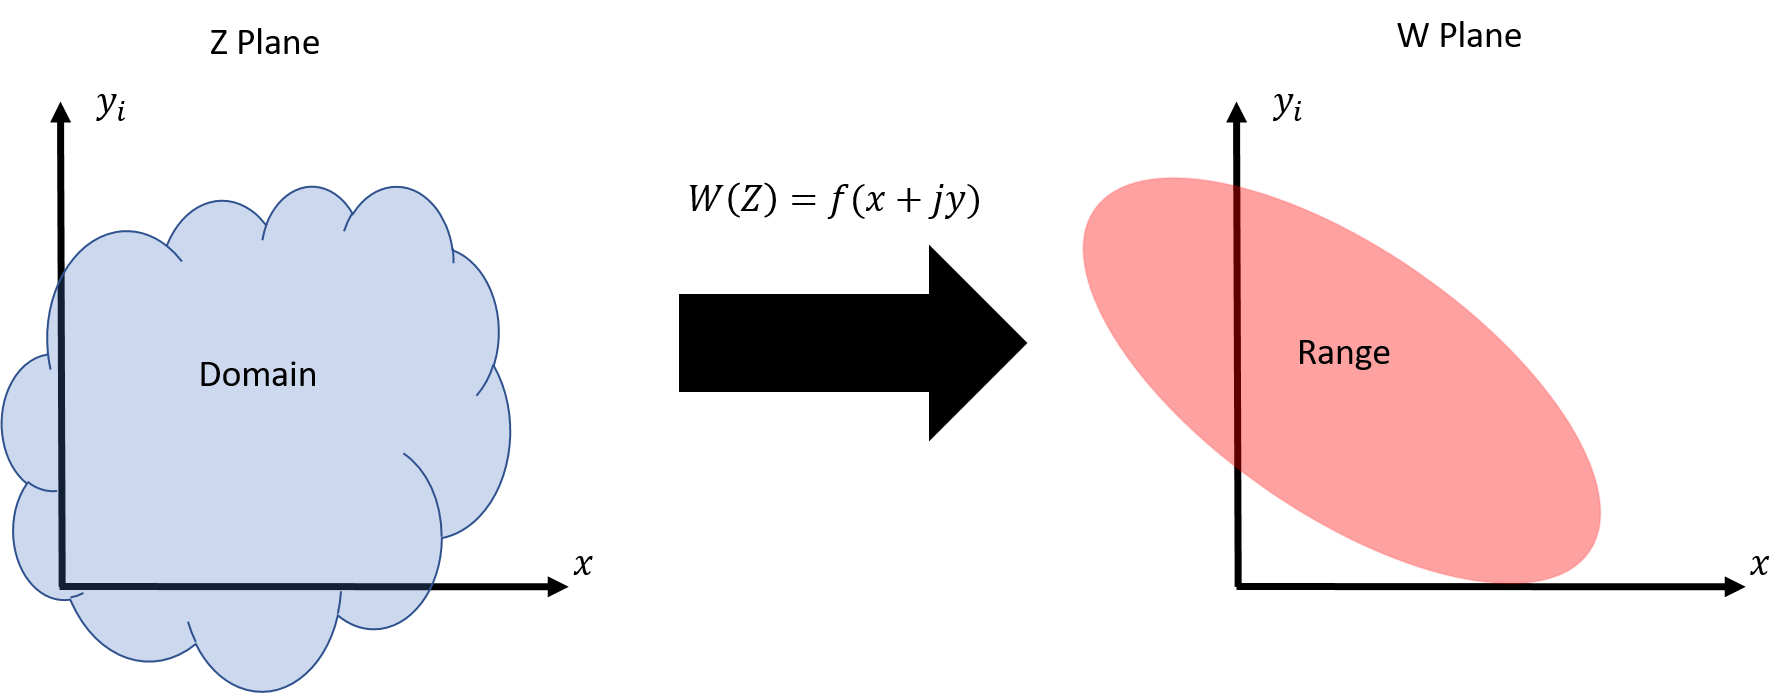
\includegraphics[width=\textwidth]{images/mapping.png}
  \caption[Illustration of complex mapping.]{An Illustration of complex mapping.}
  \label{fig:mapping}
  \end{figure}
  
  \par Let $z = x + j\,y$, where $j$ is the imaginary number $\sqrt{-1}$, then a function of $z$, such as $W(z) = u(x,y) + j\,v(x,y)$, can be considered a mapping of an area of one complex plane to an area in another complex plane (figure \ref{fig:mapping}). Conformal transformations are a special kind of mapping between two complex planes that preserves local angles. A mapping is conformal if it is composed of analytic functions, and as a consequence, fulfills the Cauchy-Rieman equations. Conformal mappings are extremely useful for solving complicated problems by mapping the problem to a simplified domain. An example of a conformal mapping is $w(z) = tan(z)$, which maps an infinite vertical strip to a circle (figure \ref{fig:circleMapping}). 

   \begin{figure}[h]
    \centering
    \begin{subfigure}[b]{0.45\textwidth}
        \centering
        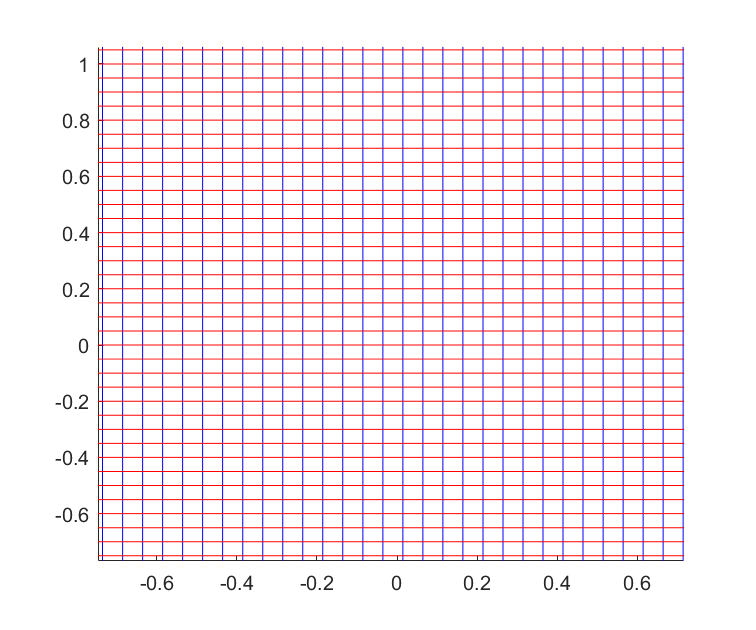
\includegraphics[width=\textwidth]{images/tanMappingStrip.png}
        \caption{Part of the partial infinite strip $-\pi/4<x<\pi/4$.}
    \end{subfigure}
    \hfill
    \begin{subfigure}[b]{0.45\textwidth}
        \centering
        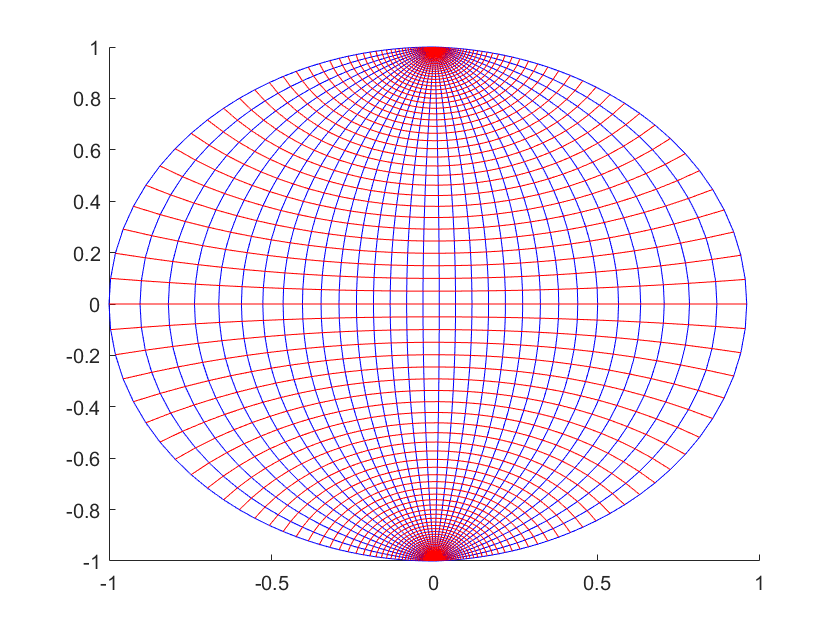
\includegraphics[width=\textwidth]{images/tanMapping.png}
        \caption{Mapping of the partial infinite vertical strip to a circle }
    \end{subfigure} 
    \caption[Conformal mapping of vertical strip to circle]{An example of conformal mapping by transforming a partial infinite vertical strip to a circle with the mapping $w(z) = tan(z)$.}
    \label{fig:circleMapping}
 \end{figure}
  
 
    \par Sun, Greene, et al. utilized the Schwartz-Christoffel transform to map the coplanar electrode configuration in figure \ref{fig:simplified_IS} to the configuration of parallel electrodes with uniform electrode fields in figure \ref{fig:parallel_capacitor} \cite{sun_analytical_2007}. The Schwartz-Christoffel formula is a powerful transform that allows the mapping of the upper complex T-plane ($y>0$) to the inside of a polygon. The formula is
    
    \begin{equation}
        Z = C_1 \int_{T_0}^T \prod^m_{r=1} (T - T_r)^{(\theta_r/\pi - 1)} dT + C_2
    \end{equation}
    
    \noindent where $Z$ is the interior of a polygon in the Z-plane with vertices $Z_1,\;Z_2,\;Z_3,\; ...,Z_m$ and angles $\theta_1,\;\theta_2,\;\theta_3,\; ...,\theta_m$ which correspond to the points $T_1,\;T_2,\;T_3,\; ...,T_m$ on the real axis of the T-plane. $C_1$ and $C_2$ are integration constants. The Schwartz-Christoffel transform has three degrees of freedom, and consequently, up to three points may be chosen arbitrarily. $T_0$ is the reference and is typically chosen at the origin.
    
    \par To find the geometric constant for coplanar electrodes, Schwartz-Christoffel transforms will be used to map the coplanar electrode geometry (Z-plane) to the upper complex plane (T-plane), and then to map the T-plane to the simplified W-plane (configuration of figure \ref{fig:parallel_capacitor}). The W-plane vastly simplifies the solution to the cell constant and the goemetric constant can be solved for with equation \ref{eqn:geometric_constant}. 
    
    \begin{figure}[h]
        \centering
        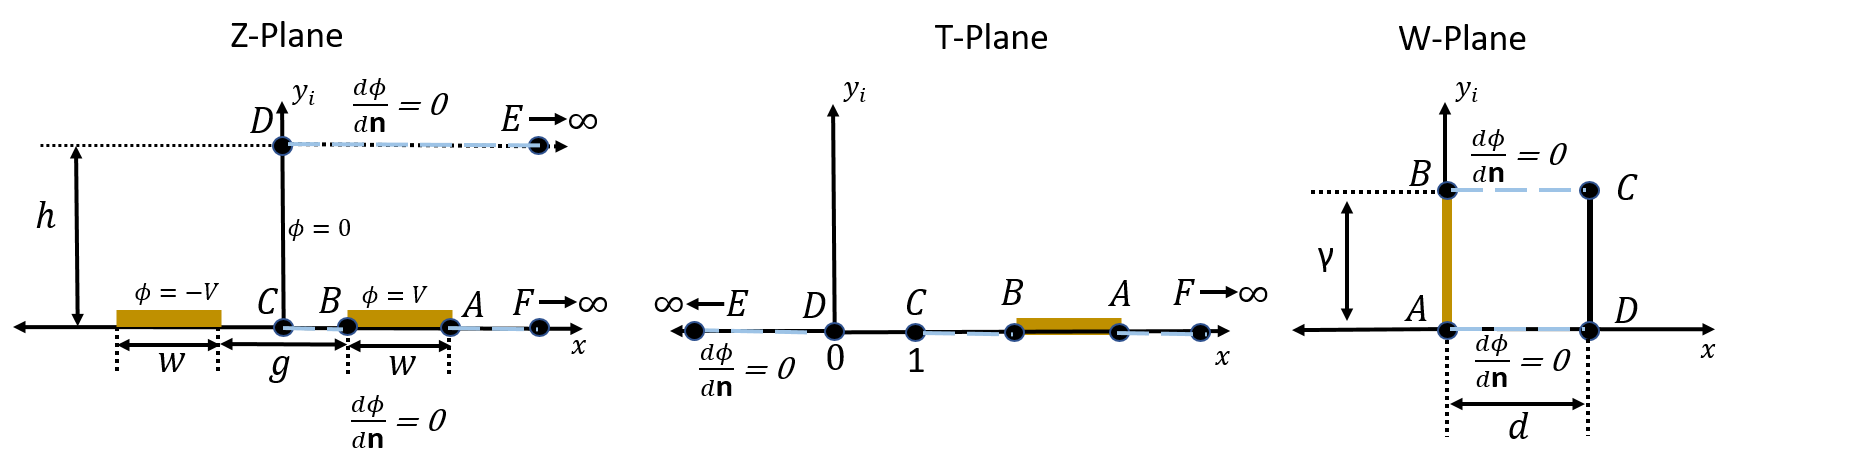
\includegraphics[width=\textwidth]{images/scmPlanes.png}
        \caption[Diagrams of coplanar electrodes through Schwartz-Christoffel mapping]{Diagrams of coplanar electrodes through Schwartz-Christoffel mapping where the Z-plane contains the physical dimensions of the electrode configuration, the T-Plane links the Schwartz-Christoffel mappins of Z and W plane, and the W-plane represents the parallel electrodes producing a uniform electrode field.}
        \label{fig:scm_planes}
    \end{figure}
    
 \subsection{Cell Suspension Equivalent Circuit}
 
 \par With a solution to the impedance of the system, an equivalent circuit of the cell and medium can be used to approximate discrete components of the medium and cell. A simple equivalent circuit was described by Foster and Schwan that describes the cell as a capacitor and resistor in series (figure \ref{fig:simple_equiv_circuit_cell_medium}) \cite{schwan_electrical_1994}. The model assumes that the resistance of the cell membrane is far greater and is shorted by the membrane reactance and can be shorted. Similarly, it is assumed that the reactance of the cytoplasm is much smaller than the cytoplasm resistance and can be neglected.
 
 \begin{figure}
     \centering
     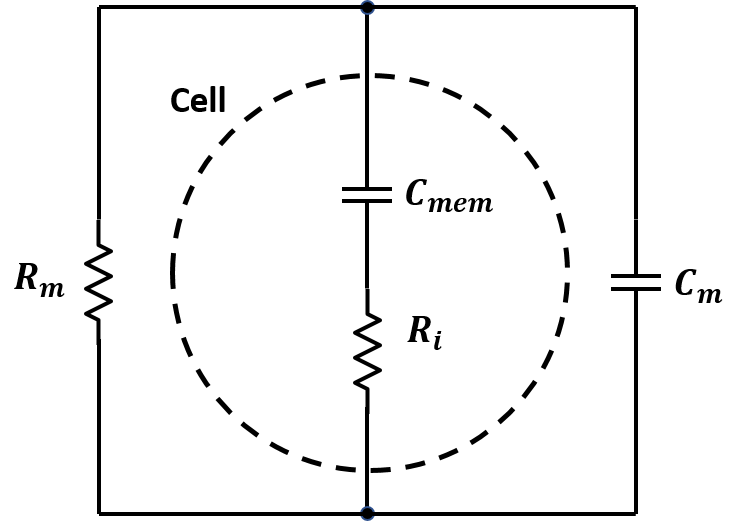
\includegraphics[width=0.5\textwidth]{images/simpleCellMediumCircuit.png}
     \caption{Simple equivalent circuit of cell and medium.}
     \label{fig:simple_equiv_circuit_cell_medium}
 \end{figure}
 
 \noindent The values of the simplified circuit model are as follow \cite{morgan_single_2007}:
 \begin{equation}
     R_m = \frac{1}{\sigma_m(1-3\Phi/2)G_f},
 \end{equation}
 \begin{equation}
     C_m = \epsilon_\infty G_f,
 \end{equation}
 \begin{equation}
     C_{mem} = \frac{9\Phi RC_{mem,0}}{4}G_f,
 \end{equation}
 \begin{equation}
     R_i = \frac{4\Big(\frac{1}{2\sigma_m}+\frac{1}{\sigma_i}\Big)}{9\Phi G_f},
 \end{equation}
 
 \noindent where $\sigma_m$ and $\sigma_i$ are the conductivities of the medium and cytoplasm respectively, $R$ is the cell radius, $\Phi$ is the volume fraction, and $C_{mem,0}$ is the specific membrane capacitance and can be expressed as \cite{sun_single-cell_2010}
 \begin{equation}
   C_{mem,0} = \epsilon_{mem}/d,
 \end{equation}
 
 \noindent where $\epsilon_{mem}$ is the permittivity of the cell membrane and d is the thickness of the membrane. $\epsilon_\infty$ is the high frequency permittivity of the suspension and can be approximated as
 \begin{equation}
     \epsilon_\infty \approx \epsilon_m \bigg[1-3\Phi\frac{\epsilon_m-\epsilon_i}{2\epsilon_m+\epsilon_i}\bigg].
 \end{equation}
 
 \par For cases where the cytoplasm reactance and membrane resistance are significant, such as during cell lysis, the complete equivalent circuit can be used (\ref{fig:complete_equiv_circuit_cell_medium}) \cite{sun_single-cell_2010}. A quantitative description of the model is described by Sun et al. \cite{sun_dielectric_2007}.

 \begin{figure}
     \centering
     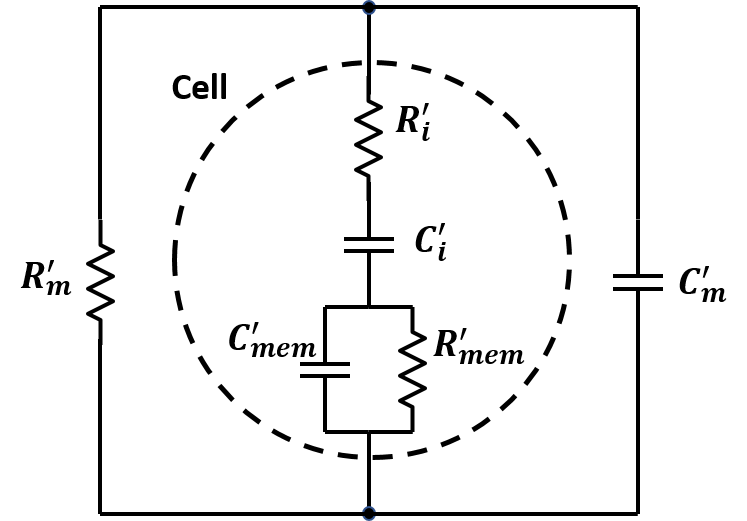
\includegraphics[width=0.5\textwidth]{images/completeCellMediumCircuit.png}
     \caption{Complete equivalent circuit of cell and medium.}
     \label{fig:complete_equiv_circuit_cell_medium}
 \end{figure}
 
 %%%%%%%%%%%%%%%%%%%%%%%%%%%%%%%%%%%%%%%%%%%%%%%%%%%%%%%%%
 % Microelectromechanical Systems and Microfluidics
 %%%%%%%%%%%%%%%%%%%%%%%%%%%%%%%%%%%%%%%%%%%%%%%%%%%%%%%%%
 \section[MEMs and Microfluidics]{MEMS and Microfluidics}
 
 \par Microelectromechanical systems (MEMS) are devices on the order of microns, and are often smaller than the diameter of a human hair (about 100 microns). MEMS evolved from the manufacturing processes used to fabricate integrated circuits and ink jet cartridges \cite{xia_soft_1998-1}. Using silicon based microfabrication techniques such as photolithography, etching, and metal deposition; mechanical and electrically driven micro-sized pumps, cantilevers, and sensors can be fabricated \cite{wang_bio-mems:_2006}. 
 
 \par Using these microfabrication techniques, systems can be miniturized in precise and reproduceable packages with applications in a variety of biology related problems. MEMS applied in these fields are referred to as BioMEMS, and is an area of rapidly growing interest and research \cite{grayson_biomems_2004}. The majority of BioMEMS are focused on creating diagnostic systems that can identify diseases and properties of biogical substances. These devices usually need to treat, filter, and utilize detection methods that include electrophoresis, dielectrophoresis, surface plasmon resonance, and enzyme-linked immunosorbent assays (ELISA) \cite{foudeh_microfluidic_2012}. In order to run diagnostics on a solution of biological material, a sample needs to undergo pretreatment, sample preparation, preconcentration and detection. With the miniaturization afforded by microfabrication technology, the concept of combining these steps into a single chip is now feasible. These devices are referred to as labs on a chip or micro total analysis systems. This thesis focuses on the detection method of such a device.
 
 %%%%%%%%%%%%%%%%%%%
 % MEMS Fabrication
 %%%%%%%%%%%%%%%%%%%
 \subsection{MEMS Fabrication}
 
 \subsection*{Photolithography}
 
 \par Photolithography is a MEMS fabrication method that patterns a thin layer of photoresist onto a substrate. Photoresist is a polymer that react to certain wavelengths of light. How the photoresist reacts determines whether the photoresist is classified as a positive or negative photoresist. Positive photoresist becomes soluble to a developer after exposure to light, and negative photoresist becomes cross-linked and insoluble to the developer after exposure. 
 
 \begin{figure}[h]
     \centering
     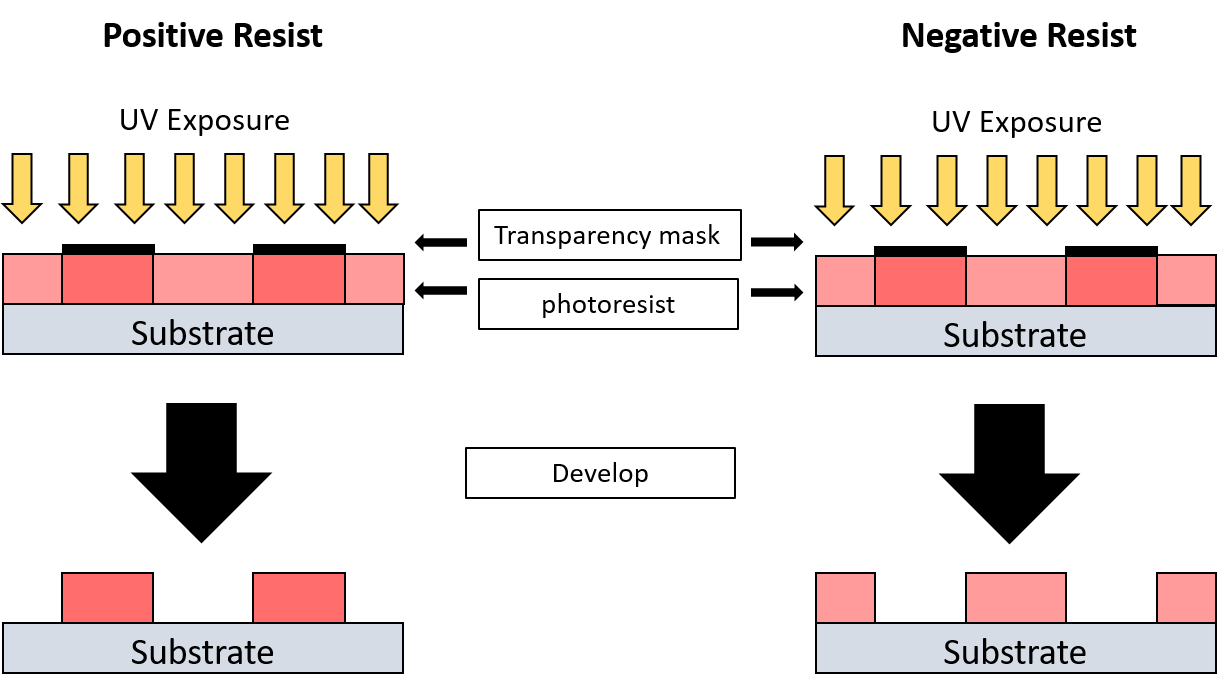
\includegraphics[width=\textwidth]{images/negative_vs_positive_resist.png}
     \caption[A comparison of positive and negative photoresist]{A comparison of positive and negative photoresist. For positive photoresist, exposed regions are removed, and for negative photoresist, unexposed regions are removed.}
     \label{fig:negative_vs_positive_resist}
 \end{figure}
 
 \par Photoresist can be evenly applied to a substrate with a precise thickness through application of a spinner machine. The machine spins the substrate at given rotation velocities to evenly distribute the photoresist and precisely control the thickness. 
 
 \par The photoresist can then be exposed to ultra violet light. In order to apply a design to the surface, a contact aligner can be used to expose the substrate under a mask. The mask is a transparency sheet with the design printed on it. The mask controls where light is allowed and the contact aligner controls the distance between the mask and the photoresist. The resist is then developed to reveal the patterned design. 
 
 \subsection*{Metal Deposition}
 
 \par One of several methods for MEMS metal deposition is sputtering. Sputtering ejects metal ions onto the target surface. The target substrate is placed on the anode with the desired metal the cathode. An argon plasma bombards the metal plate and ejects metal ions that are attracted to the anode and deposit on the target substrate. 
 
 \subsection*{Plasma Bonding}
 
 \par To irreversibly bond polydimethyl Siloxane (PDMS), the surface can be exposed to an air plasma. The plasma activates the PDMS surface by creating Si-OH groups that can bond to itself, glass, silicon, polystyrene, polyethylene, and silicon nitride \cite{mcdonald_polydimethylsiloxane_2002-1}.

 \begin{figure}[h]
     \centering
     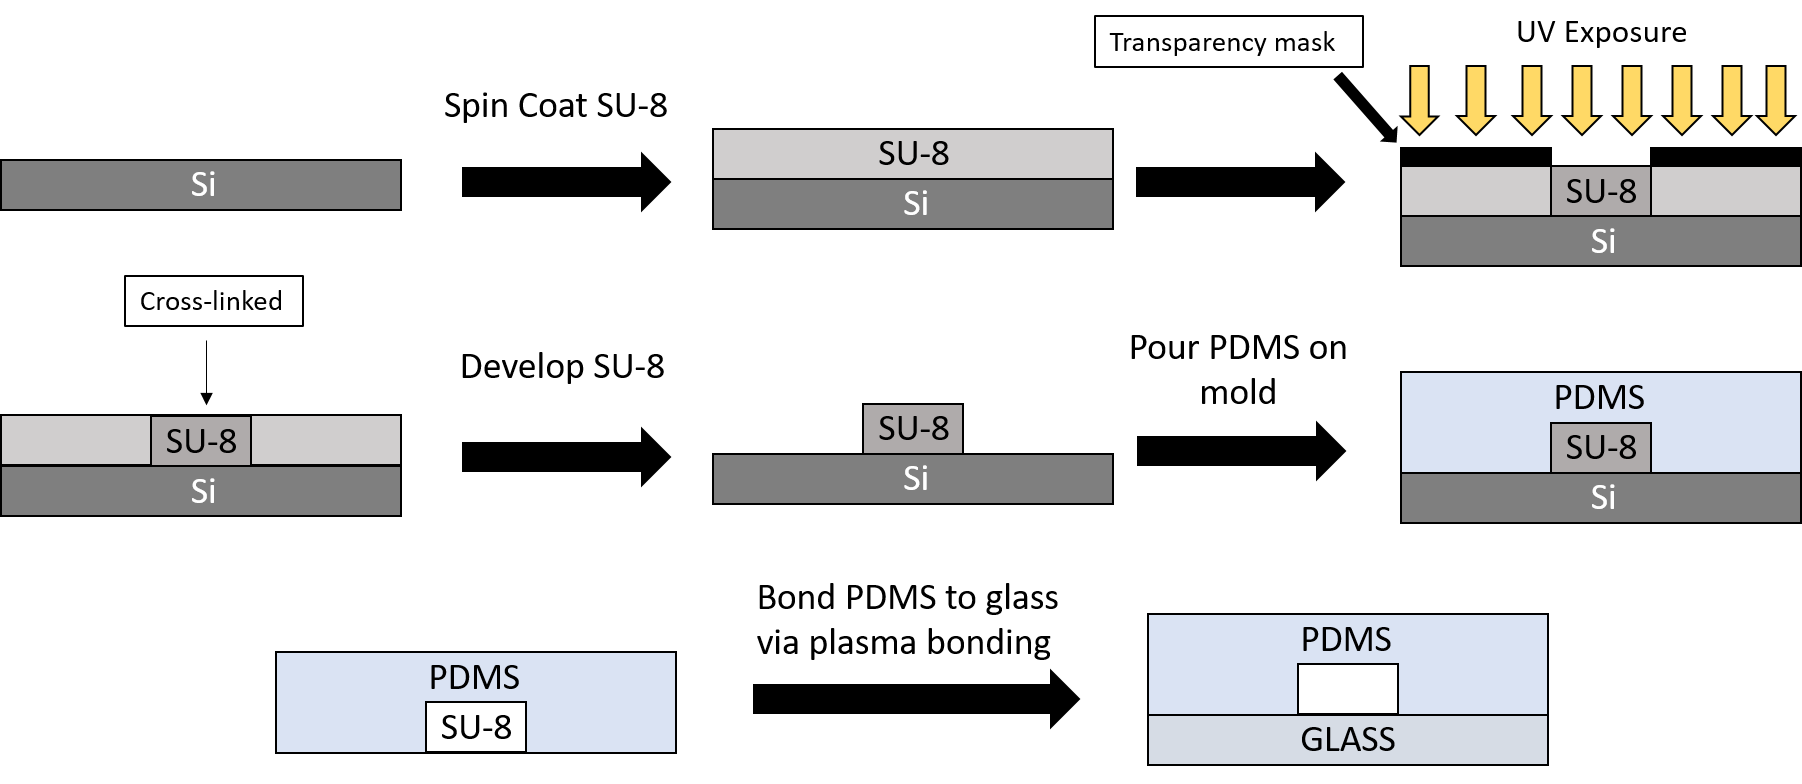
\includegraphics[width=\textwidth]{images/softLithography.png}
     \caption{Micro-channel manufacturing flowchart with SU-8 photoresist and soft-lithography.}
     \label{fig:soft_lithography}
 \end{figure}
 
 
 \subsection*{Soft-lithography}
 
 \par Soft-lithography uses photolithography to create a mold of the desired structures. A material such as PDMS can be poured over the mold and then removed to create the desired structure. The PDMS can be plasma bonded to a substrate to create fluid channels. Soft-lithography is frequently used for the fabrication of microfluidic channels since the process is far easier and cheaper than the alternative of glass etching \cite{whitesides_soft_2001}.
 
 
 \subsection*{Lift-off Process}
 
 \par The lift-off process is a method for precise metal deposition of a pattern onto a substrate and is useful for creating micro-scale electrodes. Photolithography is first used to pattern photoresist where metal is not desired. After metal deposition of the substrate with patterned photoresist, the sputtered substrate is then placed in photoresist remover to lift off the photoresist with the undesired metal. 
 
 \begin{figure}
     \centering
     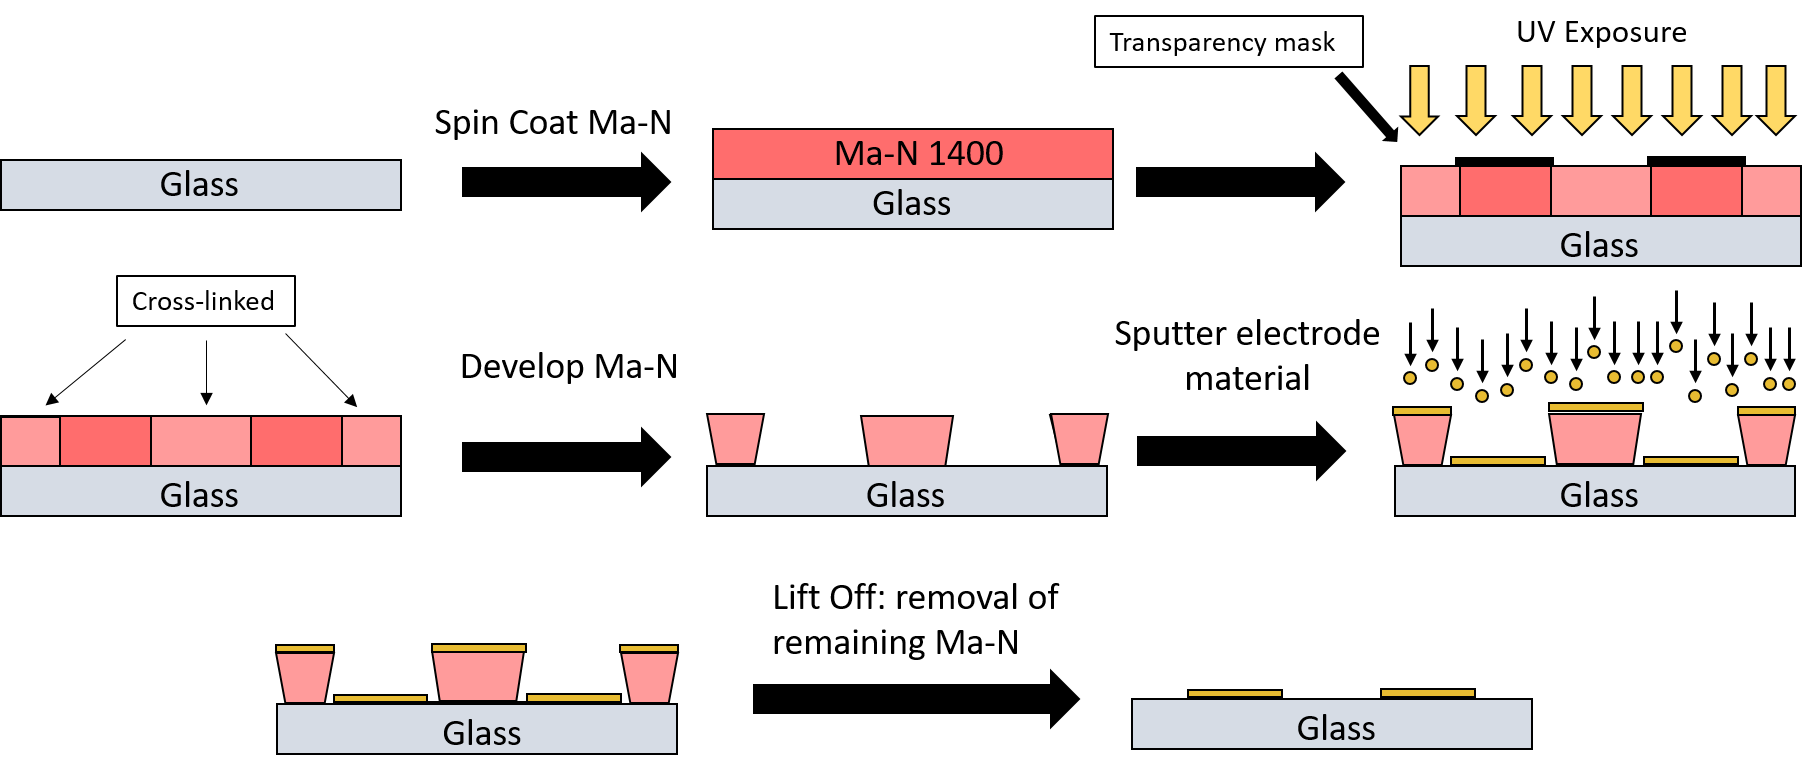
\includegraphics[width=\textwidth]{images/electrodeFabrication.png}
     \caption{Electrode fabrication flowchart through the lift off process.}
     \label{fig:lift_off}
 \end{figure}
 
 
 %%%%%%%%%%%%%%%%%%%%%%%%%%
 % Microfluidics
 %%%%%%%%%%%%%%%%%%%%%%%%%%
 \subsection{Microfluidics}
 
\par In most BioMEMS there is fluid flow on the micrometer scale. At this scale fluid flow physics differ from fluid flow at the macro scale. Understanding and leveraging microfluidic mechanics allows for small reagent and sample volumes, multiplexing, and physic phenomenon that allow experiments and functions not possible at the macro scale. Laminar flow, diffusion, fluidic resistance, surface area to volume, and surface tension, may not be dominant in phenomenon on the macro scale, but on the micro scale become significant \cite{david_j._beebe_physics_2002}. 

\subsection*{The Navier-Stokes Equation}

\par The Navier-Stokes formula is a partial differential equation that describes the fluid velocity given a set of boundary conditions. The Navier-Stokes equation is derived from applying the Newton's second law to an infinitesimally small arbitrary control volume:
\begin{equation}
    \rho \frac{\text{D}\textbf{u}}{\text{D}t} = \sum \textbf{f}
    \label{eqn:cons_momentum}
\end{equation}

\noindent where $\rho$ is the mass density, $\textbf{u}$ is the velocity vector, $\sum \textbf{f}$ is the sum of forces applied to the control volume, and $\frac{\text{D}()}{\text{D}t}$ is the material derivative \cite{probstein_physicochemical_2005}. The material derivative is the time derivative of a function that is spatially dependent and arises from the chain rule. The material derivative of an arbitrary spatial and temporal function ($F = F(t,x,y,z)$) can be calculated as
\begin{equation}
    \frac{\text{D}F}{\text{D}t} = \frac{dF}{dt} + \frac{dF}{dx}\frac{dx}{dt} + \frac{dF}{dy}\frac{dy}{dt} + \frac{dF}{dz}\frac{dz}{dt},
\end{equation}

and can be expressed as 
\begin{equation}
    \frac{\text{D}F}{\text{D}t} = \frac{dF}{dt} + \textbf{v} \cdot \boldsymbol{\nabla}F,
\end{equation}

or in index notation as
\begin{equation}
    \frac{\text{D}F}{\text{D}t} = \frac{dF}{dt} + v_j\frac{dF}{dx_j}.
\end{equation}

\noindent The material derivative is valid for scalars and vectors.

\par Surface forces are present in many fluid systems and generally arise from pressure driven flow and viscous properties of the fluid. In general, the surface forces are expressed as the divergence of the stress tensor:
\begin{equation}
    \textbf{f}_s = \boldsymbol{\nabla} \cdot \Tau
\end{equation}
\begin{equation}
    \textbf{f}_s = \frac{d\tau_{ij}}{dx_i}
\end{equation}

\noindent where $\textbf{f}_s$ is the surface force, and $\Tau$ and $\tau_{ij}$ are the second order stress tensor which is dependent on the type of fluid and the driving forces. For pressure driven inviscid fluids, the stress tensor and surface forces can be expressed as 
\begin{equation}
    \tau_{ij} = -p\delta_{ij}
\end{equation}
\begin{equation}
    \textbf{f}_s = - \frac{dp}{dx_j}
\end{equation}

\noindent where p is the pressure. 

\par For a viscid Newtonian fluid, the stress tensor and surface force can be expressed as \cite{probstein_physicochemical_2005}
\begin{equation}
    \tau_{ij} = -p\delta_{ij} + 2\mu(\epsilon_{ij} - \frac{1}{3}\epsilon_{kk}\delta_{ij})
\end{equation}
\begin{equation}
    \textbf{f}_s = \frac{dp}{dx_i} + \mu \frac{d}{dx_j}(\frac{du_i}{dx_j} + \frac{du_j}{dx_i} - \frac{2}{3}\delta_{ij}\frac{du_k}{dx_k})
    \label{eqn:viscid_newt_force}
\end{equation}

\noindent where $\epsilon_{ij}$ is the rate of strain tensor written as 
\begin{equation}
    \epsilon_{ij} = \frac{1}{2} \Big(\frac{du_i}{dx_j} + \frac{du_j}{dx_i}\Big).
\end{equation}

\noindent If the fluid is incompressible, then conservation of mass states
\begin{equation}
    \frac{du_k}{dx_k} = \boldsymbol{\nabla} \cdot \textbf{u} = 0,
    \label{eqn:incompressible_cons_mass}
\end{equation}

\noindent and equation \ref{eqn:viscid_newt_force} can be simplified to 
\begin{equation}
    \textbf{f}_s = -\frac{dp}{dx_i} + \mu \frac{d^2u_i}{dx^2_j}
\end{equation}
\begin{equation}
    \textbf{f}_s = -\boldsymbol{\nabla}p + \mu\boldsymbol{\nabla}^2\textbf{u}
    \label{eqn:viscous_pressure_force}
\end{equation}

\par Additional common forces on the control volume can include the gravitational force
\begin{equation}
    \textbf{f}_g = \rho \textbf{g},
    \label{eqn:gravity_force}
\end{equation}

\noindent where \textbf{g} is the acceleration of gravity, and for some microfluidic applications, the electroosmotic flow force (EOF)
\begin{equation}
    \textbf{f}_{EOF} = -\rho_e \boldsymbol{E},
\end{equation}

\noindent where $\boldsymbol{E}$ is the electric field vector, and $\rho_e$ is the net charge density of the electric double layer (EDL). Electric osmotic flow arises from the Coulomb force caused by the net electric charge from the electric double layer at the channel surface and the applied electric field. The electric double layer arises from the equilibrium of the solid-fluid interface \cite{kirby_micro-and_2010}. EOF results in plug flow which is characterized by a flat velocity profile in contrast to a parabolic velocity profile in pressure driven flow (figure \ref{fig:plug_vs_parabolic_flow}).

\begin{figure}[ht]
    \centering
    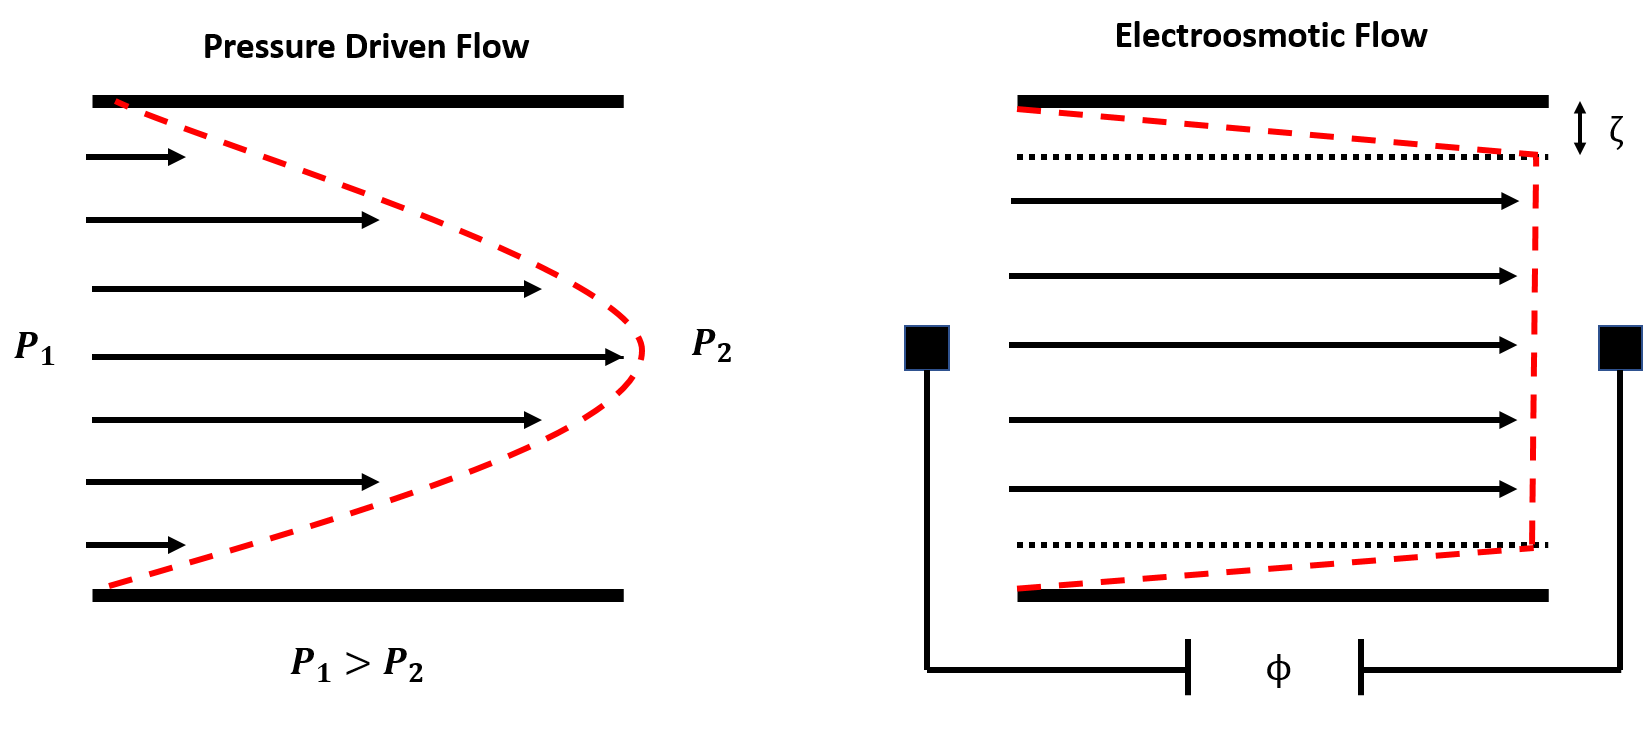
\includegraphics[width = \textwidth]{images/plugVsParabolic.png}
    \caption[Pressure driven versus electroosmotic flow profile]{Pressure driven versus electroosmotic flow profile. The pressure driven flow results in a parabolic flow profile while the electroosmotic flow with an applied voltage of $\phi$ results in a plug flow velocity profile. Near the wall of the EOF conduit in the EDL, the velocity increases until outside of the EDL there is no net charge to fight viscous forces, and the velocity profile plateus.}
    \label{fig:plug_vs_parabolic_flow}
\end{figure}

\par The most common form of the Navier-Stokes equation includes the surface forces of pressure driven Newtonian fluids with the gravitational forces, and can be expressed by combining equations \ref{eqn:cons_momentum}, \ref{eqn:viscous_pressure_force}, and \ref{eqn:gravity_force}. 
\begin{equation}
    \rho(\frac{d\textbf{u}}{dt} + \textbf{u}\cdot\boldsymbol{\nabla}\textbf{u}) = -\boldsymbol{\nabla}p + \mu\boldsymbol{\nabla}^2\textbf{u} + \rho \textbf{g}
    \label{eqn:navier_stokes}
\end{equation}

\noindent For microfluidic applications, the Navier-Stokes equation can often be simplified by assuming negligible inertial forces (Re $<<$ 2300; laminar flow) and gravitational forces allowing equation \ref{eqn:navier_stokes} to be rewritten as
\begin{equation}
        \boldsymbol{\nabla}p = \mu\boldsymbol{\nabla}^2\textbf{u}.
\end{equation}

\par Currently there is no general solution to the Navier-Stokes equation, but can be solved in specific applications with simplifying assumptions, and is widely used in computational approximations.

\subsection*{Laminar Flow}
\par Laminar flow describes the condition where the velocity of a particle in fluid flow is not a random function of time. This is in contrast to turbulent flow which is chaotic \cite{david_j._beebe_physics_2002}. The dimensionless Reynold number can quantitatively characterize a fluid flow and is a ratio of inertial and viscous forces. The Reynold number can be expressed as
\begin{equation}
    \text{Re} = \frac{\rho v L}{\mu},
\end{equation}

\noindent where $\rho$ is the fluid density, $v$ is the characteristic fluid velocity, $\mu$ is the fluid viscosity, and $L$ is the characteristic length. In many cases, the characteristic length is the hydraulic diameter ($D_h$). The hydraulic diameter is used for fluid calculations in non-circular conduits by relating the conduit to a circular geometry in a proportion that maintains the conservation of momentum of the original conduit \cite{david_j._beebe_physics_2002}.

\par The hydraulic diameter can be expressed as ratio of cross-sectional area to conduit perimeter:

\begin{equation}
    D_h = 4 \frac{A}{P},
    \label{eqn:hydraulic_diameter}
\end{equation}

\noindent where $A$ and $P$ are the cross-sectional area and perimeter of the conduit respectively. For a cylindrical conduit, equation \ref{eqn:hydraulic_diameter} simplifies to $D_h = D_c$ where $D_c$ is the diameter of a circular cross-section. For a rectangular cross-section, the hydraulic diameter is expressed as 
\begin{equation}
    D_h = \frac{2hw}{w+h},
\end{equation}

\noindent where $h$ and $w$ are the height and width of the cross-sectional rectangle respectively. For turbulent flows, where the geometry is of lesser consequence, equation \ref{eqn:hydraulic_diameter} is a good approximation for fluid calculations, but for laminar flow, specifics of the conduit geometry is of great consequence and equation \ref{eqn:hydraulic_diameter} should be used with caution.

\par In general, flow conditions with a Reynolds number much larger than 2300 exhibit turbulent behaviours, and flow conditions with a Reynolds number much smaller than 2300 exhibit laminar flow behaviours. The laminar-turbulent transition number of 2300 is reportedly accurate for microfluidics as well \cite{david_j._beebe_physics_2002}.

\par Referring back to equation \ref{eqn:hydraulic_diameter}, since the product of characteristic length and velocity for microfluidic systems, most microfluidic flows are considered laminar. An important consequence is that separate streams that come in contact will not mix via convection, but only through diffusion. This phenomenom can be quantified with the dimensionless P\'eclet number (Pe), which is defined as the ratio of convection transport to diffusion transport \cite{nguyen_micromixersreview_2005}. The P\'eclet number can be expressed as 
\begin{equation}
    \text{Pe} = \frac{vL}{D}
\end{equation}

\noindent where D is the diffusion coefficient. The P\'eclet number can also be defined with the Reynolds number
\begin{equation}
    Pe = \text{Re}\;\text{Sc}
\end{equation}

\noindent where Sc is the dimensionless Schmidt number and describes the ratio of momentum diffusivity and and mass diffusivity. The Schmidt can be calculated as
\begin{equation}
    \text{Sc} = \frac{\mu}{\rho D}
\end{equation}

\par For fluid systems where Pe is much larger than 1, the system is convection dominated and when Pe is much smaller than 1, the system is diffusion dominated. Again, the product of the characteristic velocity and length in microfluidic systems is usually very small so in most BioMEMS, the system is diffusion dominated and cannot rely on convective mixing. To facilitate mixing in microfluidic systems, the device should be designed to create large surface areas between streams to expedite the diffusion process, or stimulate turbulent flow to create convective transport.


\subsection*{Diffusion}

\par Since microfluidic flow is almost always laminar, mixing will mainly occur via diffusion (figure \ref{fig:diffusion_ilustration}) \cite{david_j._beebe_physics_2002}. Diffusion is the phenomenon where a concentration will average over a volume by Brownian motion. Fick's laws give a quantitative description of diffusion. The first law states that the molar flux of a dissolved species is proportional to the concentration gradient of that species and can be expressed as 
\begin{equation}
    \boldsymbol{J} = -D \boldsymbol{\nabla}C,
    \label{eqn:ficks_first}
\end{equation}

\noindent where $\boldsymbol{J}$ is the molar flux of a diffusive species, $\boldsymbol{\nabla}C$ is the concentration gradient, and $D$ is a proportionality factor known as the translational diffusion constant.

\par Fick's second law arises from the continuity of mass
\begin{equation}
    \frac{dC}{dt} + \boldsymbol{\nabla} \cdot \boldsymbol{J} = 0,
\end{equation}

\noindent And by substituting in Fick's first law (equation \ref{eqn:ficks_first}), Fick's second law can be expressed as 
\begin{equation}
    \frac{dc}{dt} = D\Delta C
    \label{eqn:ficks_second}
\end{equation}

\noindent Equation \ref{eqn:ficks_second} describes the time and spatial dependencies of concentrations.

\par By examining the random walk of a particle due to Brownian motion, the mean displacement of particles can be described:
\begin{equation}
    \Big< r^2 \Big> = 2 N D t
\end{equation}

\noindent where $<r^2>$ is the squared mean displacement of a particle, $N = 1$, $2$, or $3$ for analysis in 1, 2, or 3 dimensions respectively, $t$ represents the time elapsed, and $D$ is the translation diffusion constant. 

\par The translation diffusion constant is a ratio of thermal motion and viscous resistance terms and can be generally expressed as 
\begin{equation}
    D = \frac{k_bT}{\overline{f}},
\end{equation}

\noindent where $k_b$ is the boltzman constant, $T$ is the temperature, and $\overline{f}$ is the mean friction coefficient \cite{probstein_physicochemical_2005}. The mean friction coefficient arises from the average of the translation friction tensor ($f_{ij}$) components. This tensor describes the viscous force on a particle as a function of velocity:
\begin{equation}
    F_i = f_{ij}v_j
\end{equation}

\noindent where for a rigid particle
\begin{equation}
    f_{ij} = 6\pi \mu R_{ij},
\end{equation}

\noindent where $\mu$ is the fluid viscosity, and $R_{ij}$ is the translation tensor that describes the equivalent radius. For a spherical particle, $R_{ij}$ reduces to the radius of the sphere and $f_{ij}$ becomes the viscous resistance from Stokes law. In this special case, the diffusion translation constant becomes
\begin{equation}
    D_o = \frac{k_BT}{6 \pi \mu r},
\end{equation}

and is known as the Stokes-Einstein equation. For spheroid particles where the radius depends on the orientation of the particle, the mean friction coefficient can be used since brownian motion will randomly move the particle in all directions. From the translation friction tensor, the mean friction coefficient can be described as 
\begin{equation}
    \overline{f}^{-1} = \frac{1}{3}(\frac{1}{f_1} + \frac{1}{f_2} + \frac{1}{f_3})
\end{equation}

\noindent where $f_1$, $f_2$, and $f_3$ refer to the components of the main diagonal of the translation friction tensor \cite{probstein_physicochemical_2005}. 

\begin{figure}[ht]
    \centering
    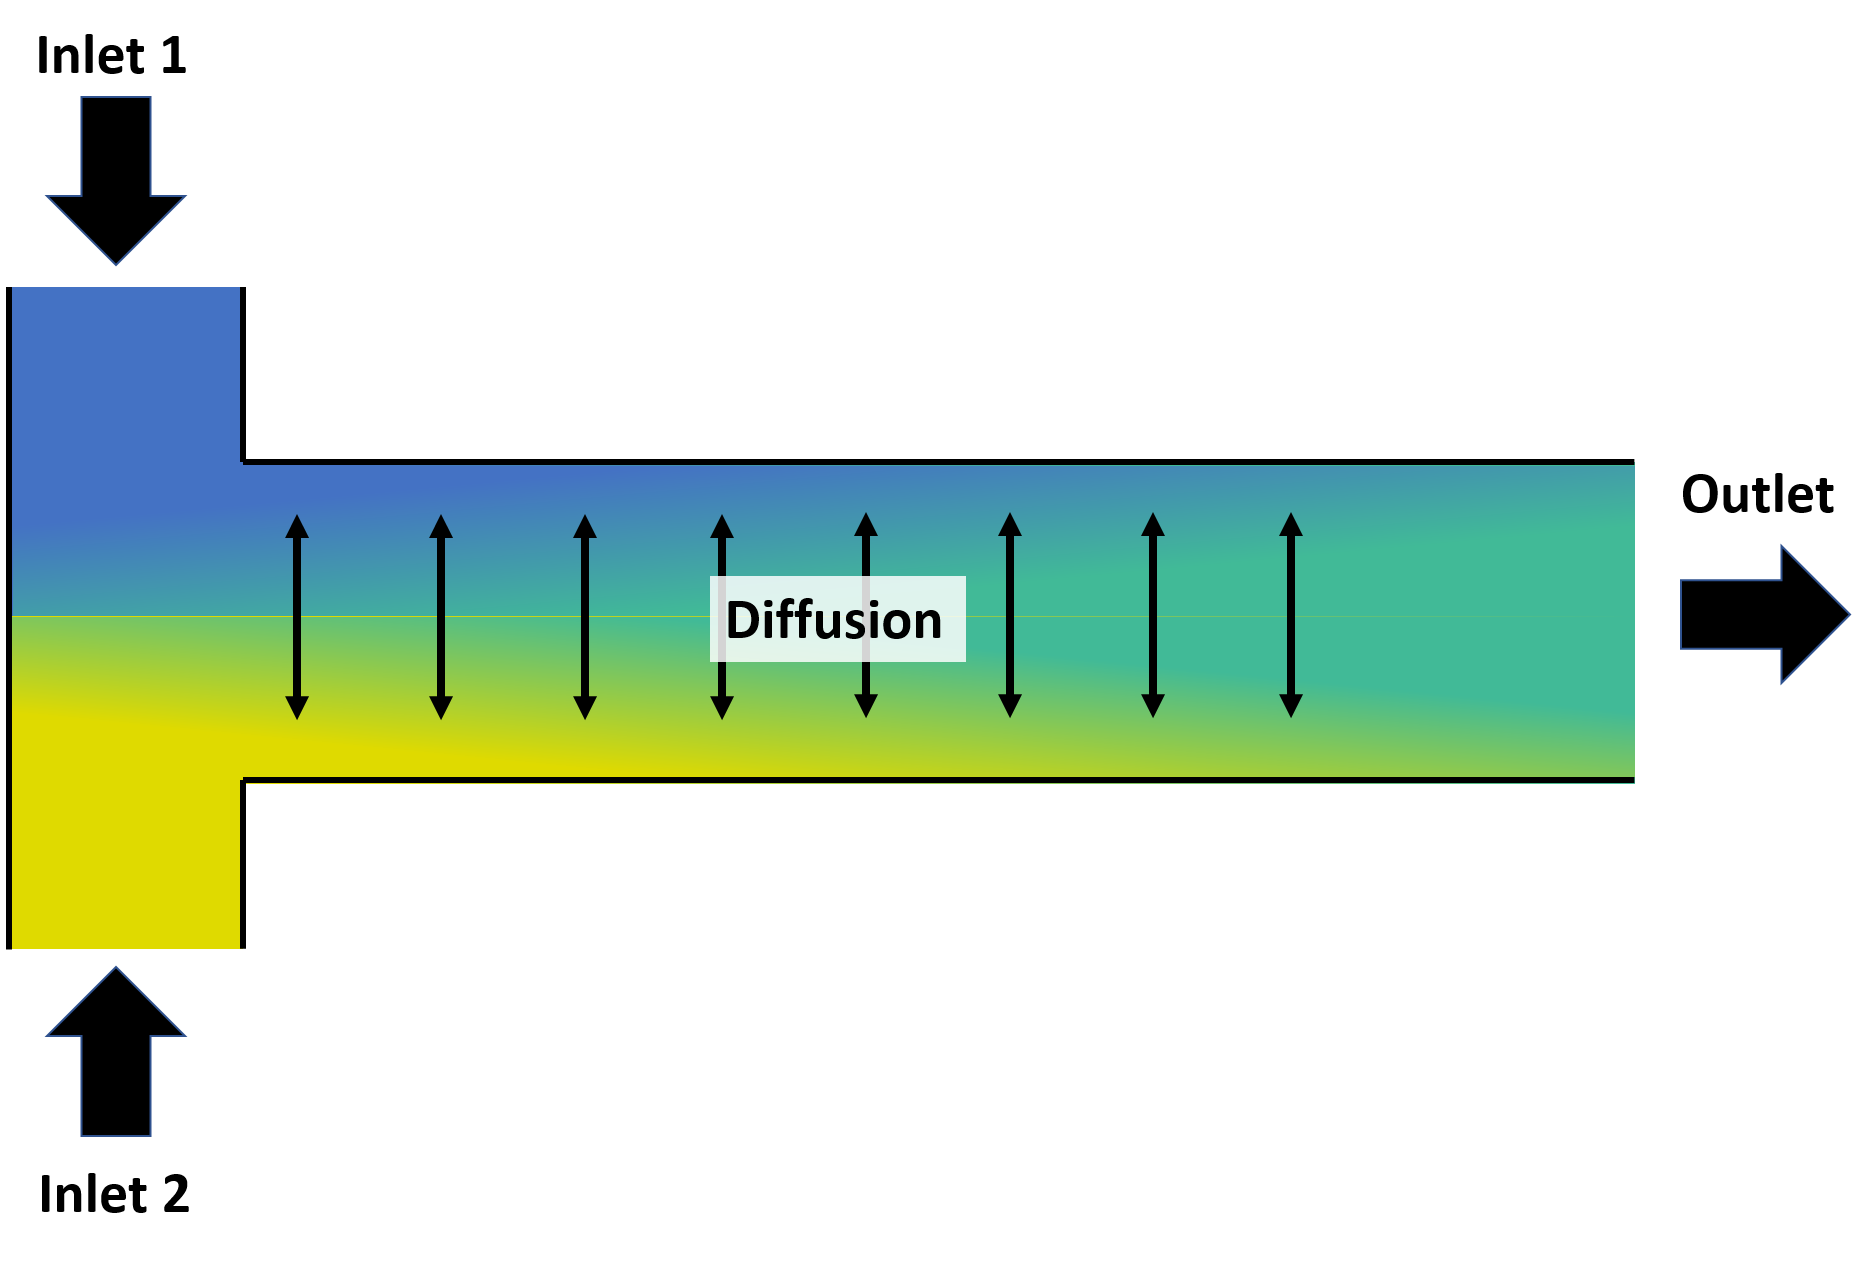
\includegraphics[width=\textwidth]{images/diffusion_illustration.png}
    \caption{Illustration of diffusion dominated transport.}
    \label{fig:diffusion_ilustration}
\end{figure} 


\subsection*{Hydraulic Resistance}

\par Fluid resistance is a powerful analogy of fluid flow to Ohm's law where pressure is analagous to electric potential, and volumetric flow rate ($Q$) is analagous to electrical current. 
\begin{equation}
    \Delta V = I R
    \label{eqn:ohm_analogy}
\end{equation}
\begin{equation}
    \Delta P = Q R
    \label{eqn:ohm_fluid}
\end{equation}

\noindent In both equation \ref{eqn:ohm_analogy} and \ref{eqn:ohm_fluid} there is a quantity referred to as the resistance that resists a flow under an applied voltage or pressure. 

\par If the velocity profile is solved for from the Navier-Stokes equation and is integrated over the volume of the conduit, the volumetric flow rate as a function of applied force can be derived. In the case of pressure-driven flow of a non-compressible Newtonian fluid through a cylindrical conduit, the Hagen-Pouisuelle equation is derived, and is expressed as
\begin{equation}
    \Delta P = Q \frac{8\mu L}{\pi R_c^4}
\end{equation}

\noindent where $L$ is the length of the conduit, $R_c$ is the radius of the conduit, and $\mu$ is the viscosity. In the case of Hagen-Pouisuelle flow, the hydraulic resistance is 
\begin{equation}
    R = \frac{8\mu L}{\pi R_c^4}.
\end{equation}

\par In the case of a rectangular conduit, the hydraulic resistance can be expressed as
\begin{equation}
    R = \frac{12\mu L}{wh^3}\Bigg[1 - \frac{h}{w}\bigg( \frac{192}{\pi^5} \sum_{n=1,3,5}^\infty \frac{1}{n^5} \tanh\Big(\frac{n\pi w}{2h}\Big) \bigg) \Bigg]^{-1},
\end{equation}

\noindent where $w$ and $h$ are the cross-sectional width and height of conduit respectively \cite{david_j._beebe_physics_2002}. If the width is far greater or smaller than the width, the hydraulic resistance can be expressed by a much simpler expression \cite{david_j._beebe_physics_2002}:
\begin{equation}
    R = \frac{12 \mu L}{wh^3} 
\end{equation}

\par The Ohm's law analogy of fluid flow can be expanded to other circuit techniques such as equivalent parallel and series resistors, and Krichoff's current and voltage laws. This analogy allows the design of complicated fluid networks at the system level.

%%%%%%%%%%%%%%%%%%%%%%%%%%%%%%%%%%%%%%%%%%%%%%%%%%%%%%%%%%%%%%%%%%%%
% The Electric Double Layer
%%%%%%%%%%%%%%%%%%%%%%%%%%%%%%%%%%%%%%%%%%%%%%%%%%%%%%%%%%%%%%%%%%%%
\section{The Electric Double Layer}
\label{sec:the_electric_double_layer}

\par When electric fields are applied to ionic solutions, the electrodes will attract ions of opposite charge. With equilibrium to thermal forces, the applied field will result in the electric double layer (figure \ref{fig:electric_double_layer}) \cite{ishai_electrode_2013}. The electric double layer creates an effective capacitance at the electrode-fluid interface. For electrodes with large surface areas, the capacitance may be large enough to be negligible, but for MEMS with micro-scale electrodes, the capacitance will be small and can mask the impedance of the device under testing for frequencies up to 100 kHz to 1 MHz \cite{bordi_reduction_2001}. 

\subsection{Theoretical Capacitance}

%%%
% Add in : Although several theoretical formulas attempt to approximate the the electric double layer, there are no physical descriptions that adequately account for the electric double layer. 
%%%

\begin{figure}[h]
    \centering
    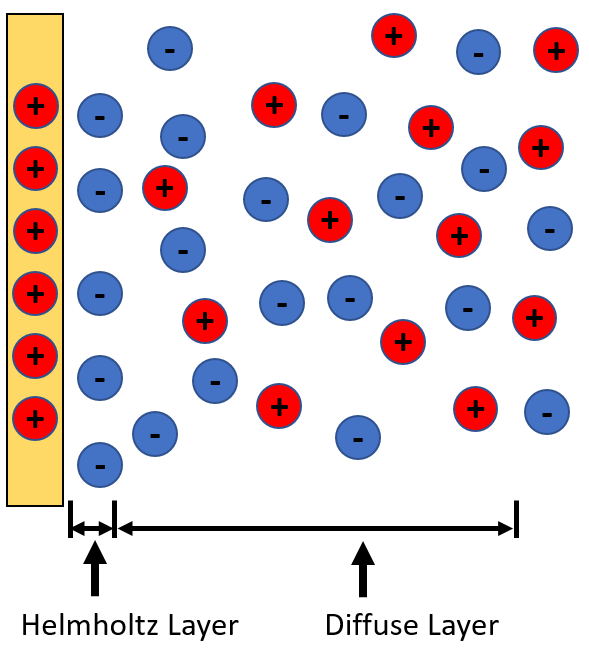
\includegraphics[width=0.7\textwidth]{images/electricDoubleLayer.png}
    \caption[Stern model of the electric double layer]{The Stern model of the electric double layer that includes the Helmholtz and diffuse layers.}
    \label{fig:electric_double_layer}
\end{figure}

\par Helmholtz was the first to describe the electric double layer and modeled it as a single layer of ions adsorbed to the surface of the electrode \cite{ishai_electrode_2013}. If the ions are treated as point charges, the Helmholtz model can be interpreted as a parallel capacitor with a distance $d_H$ between the plates that represents the distance between the center of the ion and the surface of the electrode. The capacitance per unit area can be approximated as

\begin{equation}
    C = \frac{\epsilon_o\epsilon_r}{d_H}
\end{equation}

\noindent where $\epsilon_o$ is the permittivity of the vacuum, $\epsilon_r$ is the relative permittivity of the medium, and $d_H$ is the thickness of the Helmholtz layer \cite{_gongadze.pdf_????}. The Helmholtz model neglects the thermal, concentration, and voltage dependencies that experiments have confirmed \cite{_jes2011.pdf_????}.

\par Guoy and Chapman expanded on the electric double layer by including the effects of thermal motion, concentration, and applied voltage \cite{chapman_li._1913,_gongadze.pdf_????}. This results in a diffuse layer that consists of counter-ions and co-ions. The distribution of ions in the diffuse layer can be described by the Boltzmann distribution:
\begin{equation}
    n_{i\pm} = n_i^o \text{exp}\Big(\frac{ \mp z_i e\phi}{k_b T}\Big),
\end{equation}

\noindent where $n_i$ is the concentration of the ion $i$, $\phi$ is the electric potential, $T$ is the temperature, $k_b$ is the Boltzmann constant, $z_i$ is the charge number of the ion, and $e$ is the charge of an electron. The charge density can be written as the sum of all ions:
\begin{equation}
    \rho(x) = e \sum_i n_i^o z_i \text{exp}\Big(\frac{-z_i e\phi}{k_b T}\Big)
\end{equation}

\par Combining Poisson's equation with the charge distribution above, results in the Poisson-Boltzmann equation:
\begin{equation}
    \nabla^2\phi = \frac{e}{\epsilon_o\epsilon_r} \sum_i n_i^o z_i \text{exp}\Big(\frac{-z_i e \phi}{k_b T}\Big),
    \label{eqn:pb_equation}
\end{equation}

\noindent and then recognizing that
\begin{equation}
    \frac{d^2\phi}{dx^2} = \frac{1}{2}\frac{d}{dx}\Big(\frac{d\phi}{dx}\Big)^2,
\end{equation}

\noindent then with the boundary condition for electrodes far apart, $\phi\to0$ and $\frac{d\phi}{dx}\to 0$ as $x\to\infty$, equation \ref{eqn:pb_equation} can be integrated to
\begin{equation}
    \Big(\frac{d\phi}{dx}\Big)^2 = \frac{2k_b T}{\epsilon_o\epsilon_r} \sum n_i^o \bigg[exp\Big(\frac{-z_i e\phi}{k_b T}\Big) - 1\bigg] 
\end{equation}

\noindent For a symmetrical electrolyte, the Poisson-Boltzmann equation can be expressed as
\begin{equation}
    \frac{d\phi}{dx} = \frac{8k_bTn^o}{\epsilon_o\epsilon_r}\sinh\Big(\frac{ze\phi}{2k_bT}\Big)
    \label{eqn:edl_efield}
\end{equation}

\noindent Capacitance can generally be defined as the differential capacitance:
\begin{equation}
    C_{diff} = \frac{d\sigma}{d\phi_o}
\end{equation}

\noindent where $\sigma$ is the surface charge of the electrode and $\phi_o$ is the electric surface potential. From Gauss's law and equation \ref{eqn:edl_efield}, the charge for the electric double layer is
\begin{equation}
    \sigma = \epsilon_o\epsilon_r \Big[\frac{d\phi}{dx}\Big]_{x=0} = \sqrt{8k_bTn_i^o\epsilon_o\epsilon_r}\sinh\Big(\frac{ze\phi_o}{2k_bT}\Big).
    \label{eqn:edl_surface_charge}
\end{equation}

\noindent Differentiating \ref{eqn:edl_surface_charge} with respect to surface potential gives the differential capacitance of the electric double layer:
\begin{equation}
    C_{GC} = \Big(\frac{2z^2e^2n_i^o\epsilon_r\epsilon_o}{k_bT}\Big)\cosh\Big(\frac{ze\phi_o}{2k_bT}\Big)
\end{equation}

\par Stern combined the Helmholtz and the Guoy-Chapman thoeries to create a model with two layers: the inner layer known as the Stern layer, which consists of the adsorbed ions on the electrode surface from the Helmholtz model, and the outer diffuse layer (figure \ref{fig:electric_double_layer} \cite{_jes2011.pdf_????}. The capacitance of the Stern model can be approximated by the capacitance of the Helmholtz and Guoy-Chapman models in series \cite{_gongadze.pdf_????}:

\begin{equation}
    C_s = \bigg[ \frac{1}{C_H} + \frac{1}{C_{GC}}\bigg]^{-1}
\end{equation}

\par Unfortunately, these models do not fully describe the electric double layer and significantly overestimates the electric double layer capacitance. Gongadze et al. measured the capacitance of the electric double layer in a phosphate-buffered electrolyte solution with titanium electrodes. Using theory, the electric double layer capacitance was calculated as 231.7 $\mu$F/cm$^2$, 77.16 $\mu$F/cm$^2$, and 57.92 $\mu$F/cm$^2$ for the Helmholtz, Guoy-Chapman, and Stern model respectively, but the experimental capacitance was 6 $\mu$F/cm$^2$ \cite{_gongadze.pdf_????}. Predicting the electric double layer is convoluted by the surface properties of the electrodes, electrochemical reactions, and other non-quantified phenomena in the solution. 

\subsection{Correction for the Electric Double Layer}

\par To overcome the theoretical shortcomings, devices can be designed to minimize the effect of the electric double layer and/or an empirical corrective function can be applied to data. Physical compensations include four electrode sample cells, increasing the surface area by coating the electrode in black platinum or polypyrrole polystyrenesulphonate, and high current density methods \cite{ishai_electrode_2013}. However, due to a combination of device constraints, difficulty in implementation, reduced electrode strength, and failure to completely bypass the electric double layer, physical compensations areusually avoided \cite{ishai_assessment_2012}. 

\begin{figure}
    \centering
    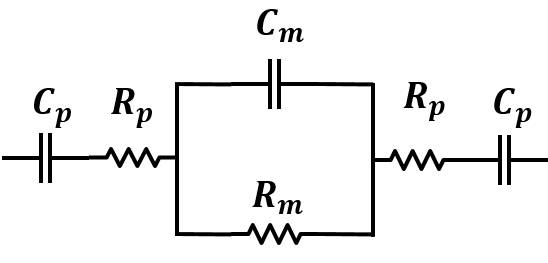
\includegraphics[width=0.5\textwidth]{images/edl_cap_equiv.png}
    \caption{A series resistor and capacitor equivalent circuit of the electric double layer.}
    \label{fig:edl_cap_equiv}
\end{figure}

\par Empirical recalculations involve fitting a reference measurement to a function or equivalent circuit. One of the more common equivalent circuit models of the electric double layer is a resistor and capacitor in series (figure \ref{fig:edl_cap_equiv}) \cite{feldman_fractal-polarization_1998}. The impedance of the system can be expressed as
\begin{equation}[h]
    Z = 2Z_p + Z_m
\end{equation}
\begin{equation}
    Z_p = \frac{1 + sC_pR_p}{sC_p}
\end{equation}
\begin{equation}
    Z_m = \frac{R_m}{sC_mR_m+1}
\end{equation}

\noindent where $Z_p$, $C_p$, and $R_p$ are the impedance, capacitance, and resistance of the electric double layer respectively; and $Z_m$, $C_m$, and $R_m$ are the impedance, capacitance, and resistance of the medium respectively. $s$ is the Laplace variable, and since our interest is in the steady state behaviour, $s = iw$.

\begin{figure}[h]
    \centering
    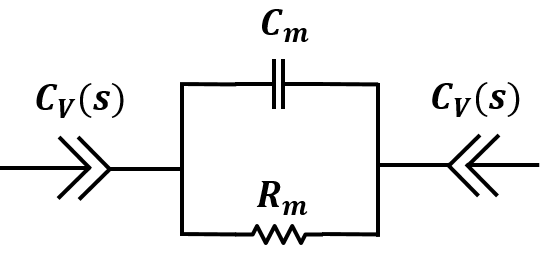
\includegraphics[width=0.5\textwidth]{images/edl_recap_equiv.png}
    \caption{A recap equivalent circuit of the electric double layer.}
    \label{fig:edl_recap_equiv}
\end{figure}


\par A second equivalent circuit involves a similar system, but with the inclusion of recap elements (figure \ref{fig:edl_recap_equiv}) \cite{feldman_fractal-polarization_1998-1}. A recap element can be modeled as 
\begin{equation}
    C_v = R(RC)^{-v}s^{-v}
\end{equation}

\noindent where C is capacitance, R is resistance, and $v$ is $0<v<1$. $v$ determines the degree of capacitance or resistance behavior, with $v=1$ a complete capacitor, and $v=0$ a pure resistor. The recap element is known as a type of constant phase element (CPE), which is named after its property of contributing a constant angle and describes an imperfect dielectric. Constant phase elements are found in a wide range of electrodes and are used extensively in empirical descriptions of electrode polarization.\cite{ishai_electrode_2013}. To fit data to the CPE, it is useful to express the system impedance as
\begin{equation}
    Z_{sys} = Z_{bulk} + Z_0\bigg(i\frac{f}{f_0}\bigg)^{-v}
\end{equation}

\noindent where $Z_{bulk}$ is the impedance of the medium, $i$ is the imaginary number, $f$ is frequency, $f_0$ is the onset frequency of the electrode polarization, and $Z_0$ is a impedance fitting term. It is convenient to find the onset frequency by looking for the characteristic tail of the CPE on a nyquist plot (figure \ref{fig:nyquist_onset}).

\begin{figure}[h]
    \centering
    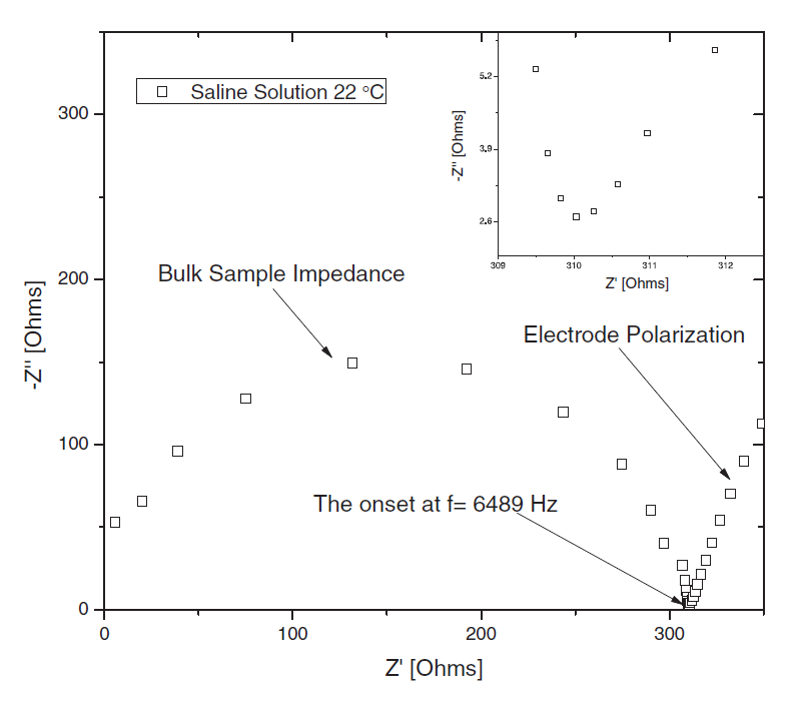
\includegraphics[width=\textwidth]{images/nyquist_ep_onset.png}
    \caption[Electrode polarization on a Nyquist plot]{Electrode polarization on a Nyquist plot with Z' and Z'' the real and imaginary components of the impedance respectively. The onset frequency of the electrode polarization can be identified by the beginning of the characteristic CPE tail \cite{ishai_assessment_2012}.}
    \label{fig:nyquist_onset}
\end{figure}


%%ist %%%%%%%%%%%%%%%%%%%%%%%%%%%%%%%%%%%%%%%%%%%%%%%%%%%%%%%%%%
 % Previous Work on the Cal Poly Biofluidic Lab's EIS System
 %%%%%%%%%%%%%%%%%%%%%%%%%%%%%%%%%%%%%%%%%%%%%%%%%%%%%%%%%%%%%%%%%%%
 %\section{Previous Work on the Cal Poly Biofluidic Lab's EIS System}
 
 % In 2009 Josh Fadriuela and Stephanie Hernandez fulfilled their thesis under Dr.Clague to create a cell impedance sensor system. Their work will be the foundation for this thesis \cite{fadriquela_design_2009-1}, \cite{hernandez_single_2009-1}.
 

%\chapter{Methods}
%
\section{Device Manufacturing}

\subsection{PDMS Channel Fabrication}
\par The device microchannels were fabricated by pouring PDMS (polydimethysiloxane) over a silicon wafer master mold. Through photolithography, a master mold was created by patterning a silicon wafer with SU-8 photoresist in  a process known as soft lithography. A 6"x6" 20,000 DPI negative transparency mask was ordered from CAD/Art Services Inc. with the emulsion face down. A general process flow is depicted in figure \ref{fig:soft_lithography}.


\subsection*{SU-8 Master Mold}

\par Before photolithography, silicon wafers were cleaned in a Piranha bath ( 98\% sulfuric acid, get pirahna def) for 15 minutes and then rinsed in DI (deionized) water, and dipped in BOE solution (get BOE def) for 5 minutes and then rinsed in DI water. The wafers were then washed and dried in the SRD (spin rinse dry) machine before baking the wafers at 205$^\circ$ for 10 minutes on a hot plate to dehydrate the wafers, and allowed to cool for 10 minutes. 

\begin{figure}[h]
    \centering
    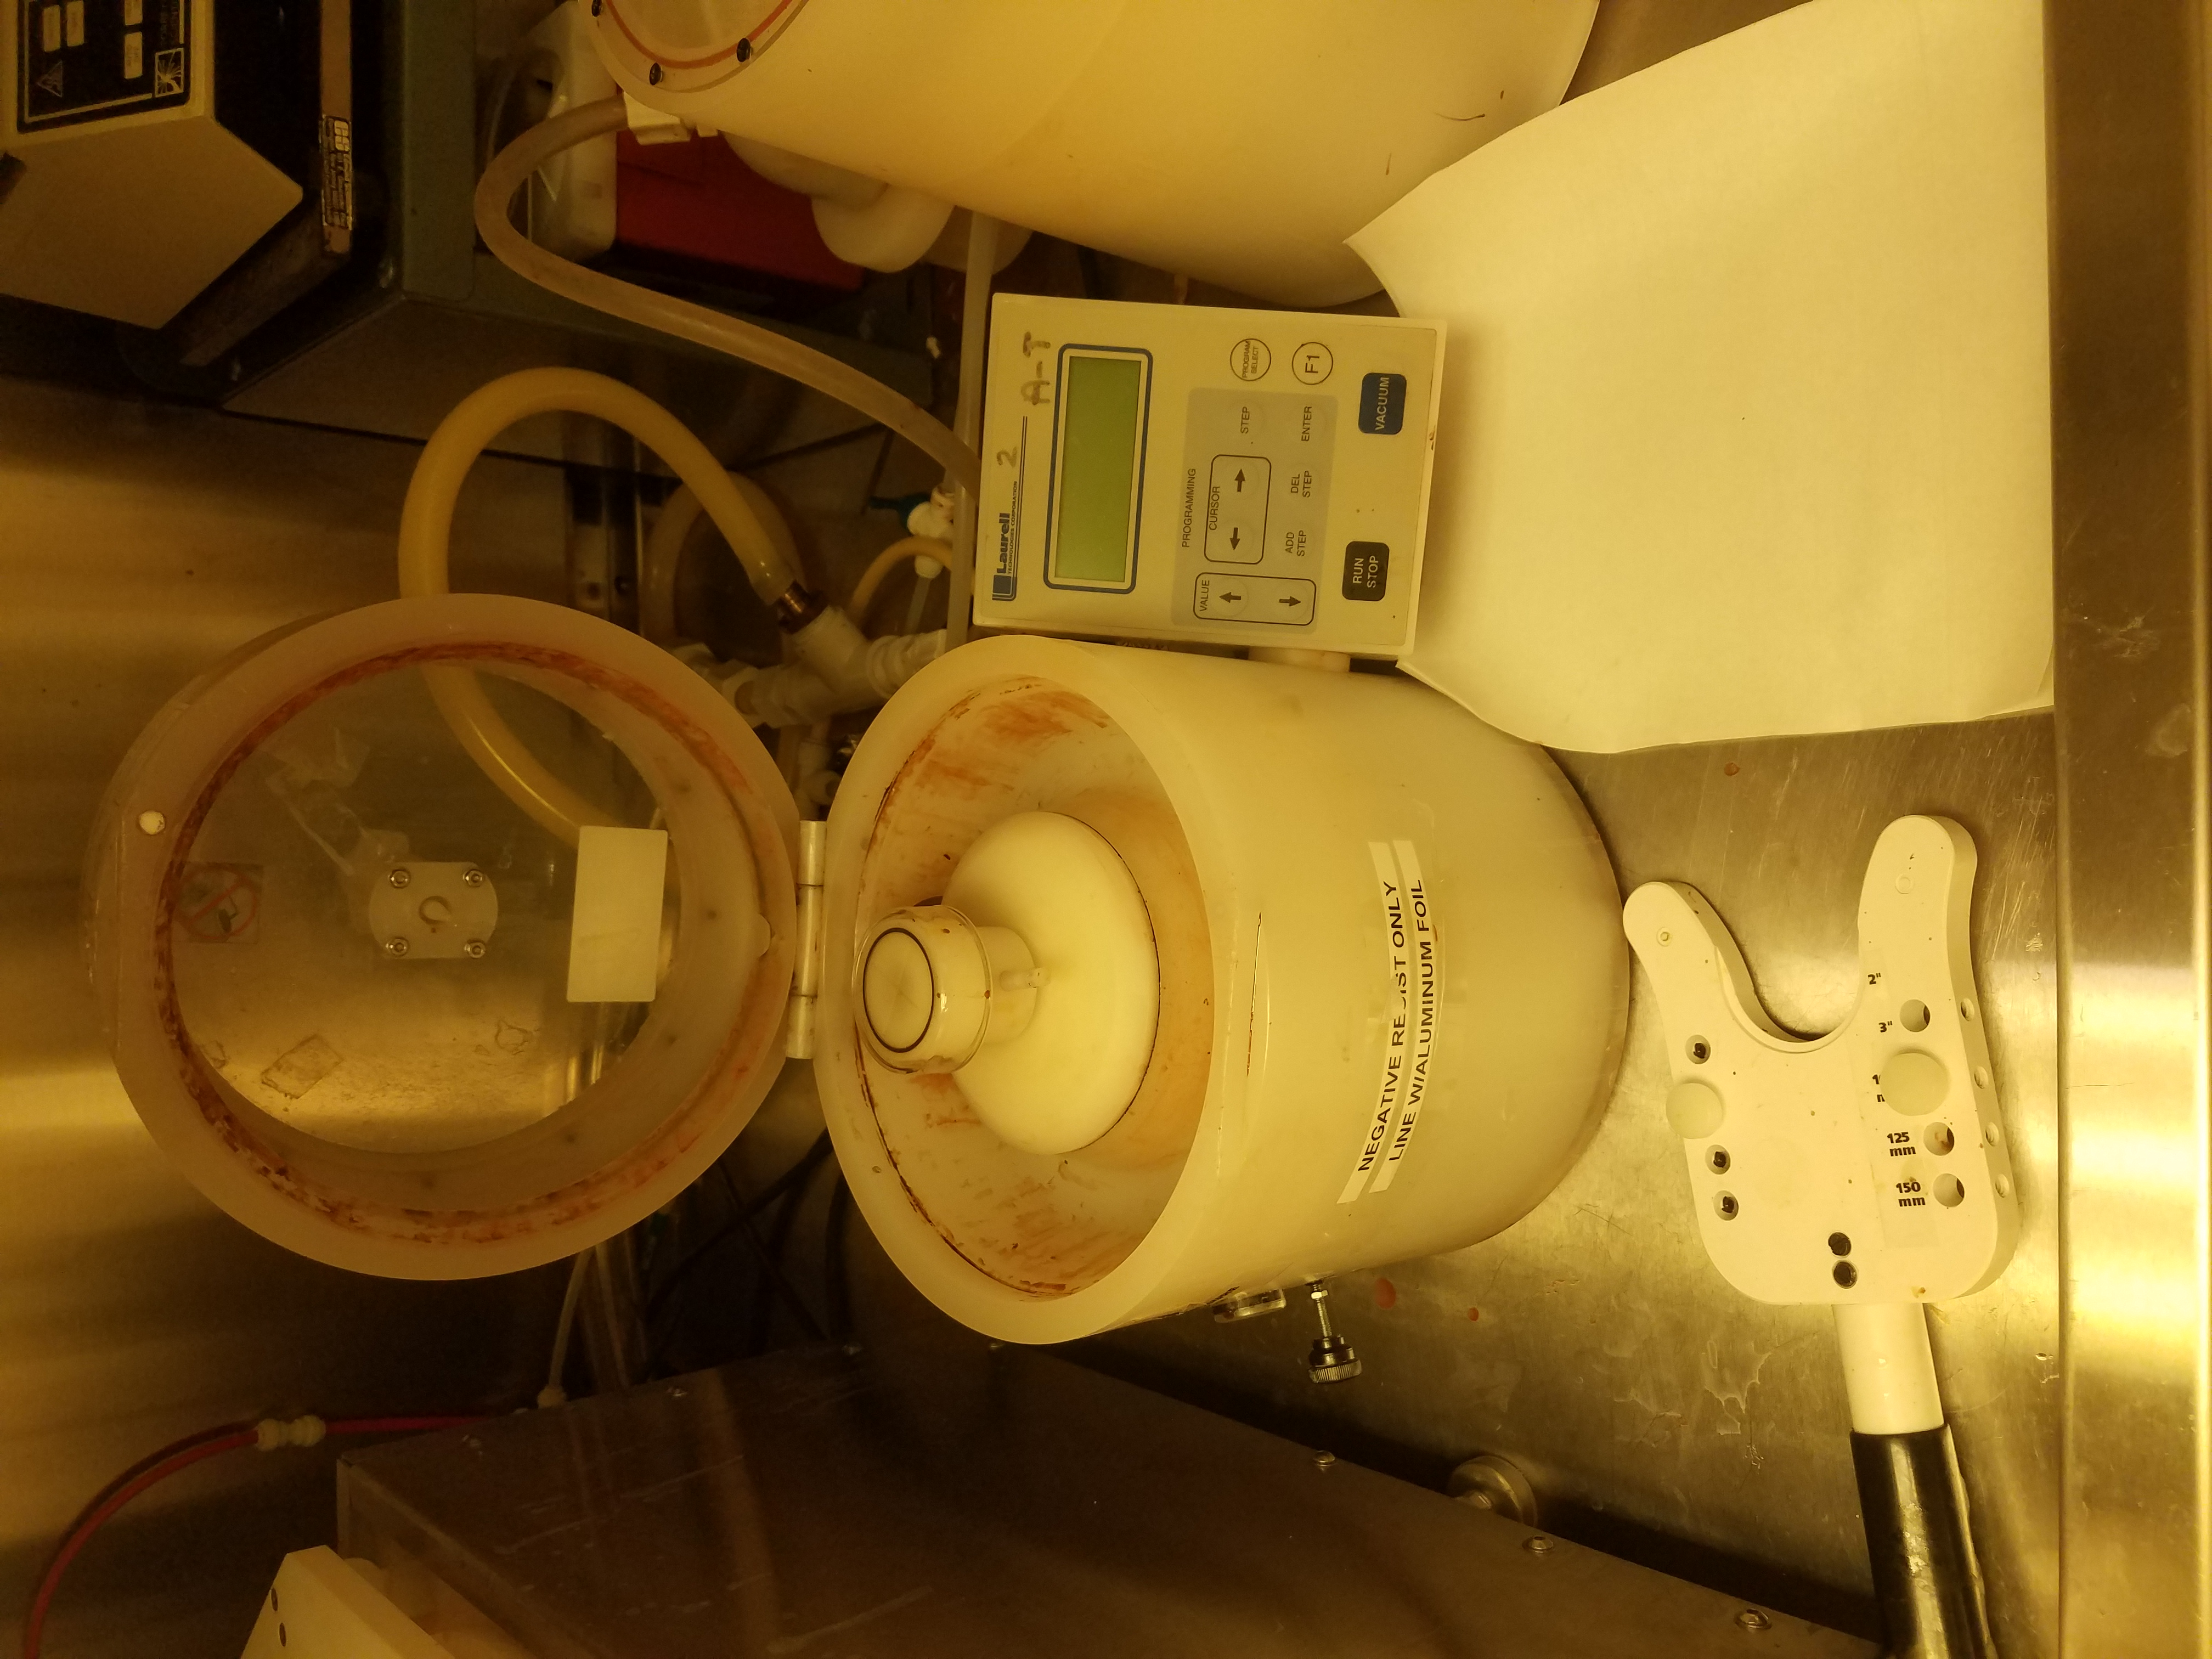
\includegraphics[width=0.7\textwidth]{images/resist_spinner_open.jpg}
    \caption{Laurel Technologiers ws-400 spin coater}
    \label{fig:spin_coater}
\end{figure}

\par The wafers were coated with SU-8 (a negative tone photoresist) on a spin coater (Laurel Technologies, ws-400; figure \ref{fig:spin_coater}). The spin coater rotates at a series of specific angular velocities in order to coat the wafer with the desired thickness of photoresist. About 4 mL of SU-8 2007 (\#07110769, MicroChem) was placed on the center of the wafer and then spun for 400 RPM for 20 seconds to disperse the SU-8, and then at 1500 RPM for 35 seconds to spread the photoresist to a 10 $\mu$m thickness. After spin-coating, the wafer was soft-baked at 85$^\circ$C for 3 minutes and allowed to cool for 4 minutes.

\begin{figure}[h]
    \centering
    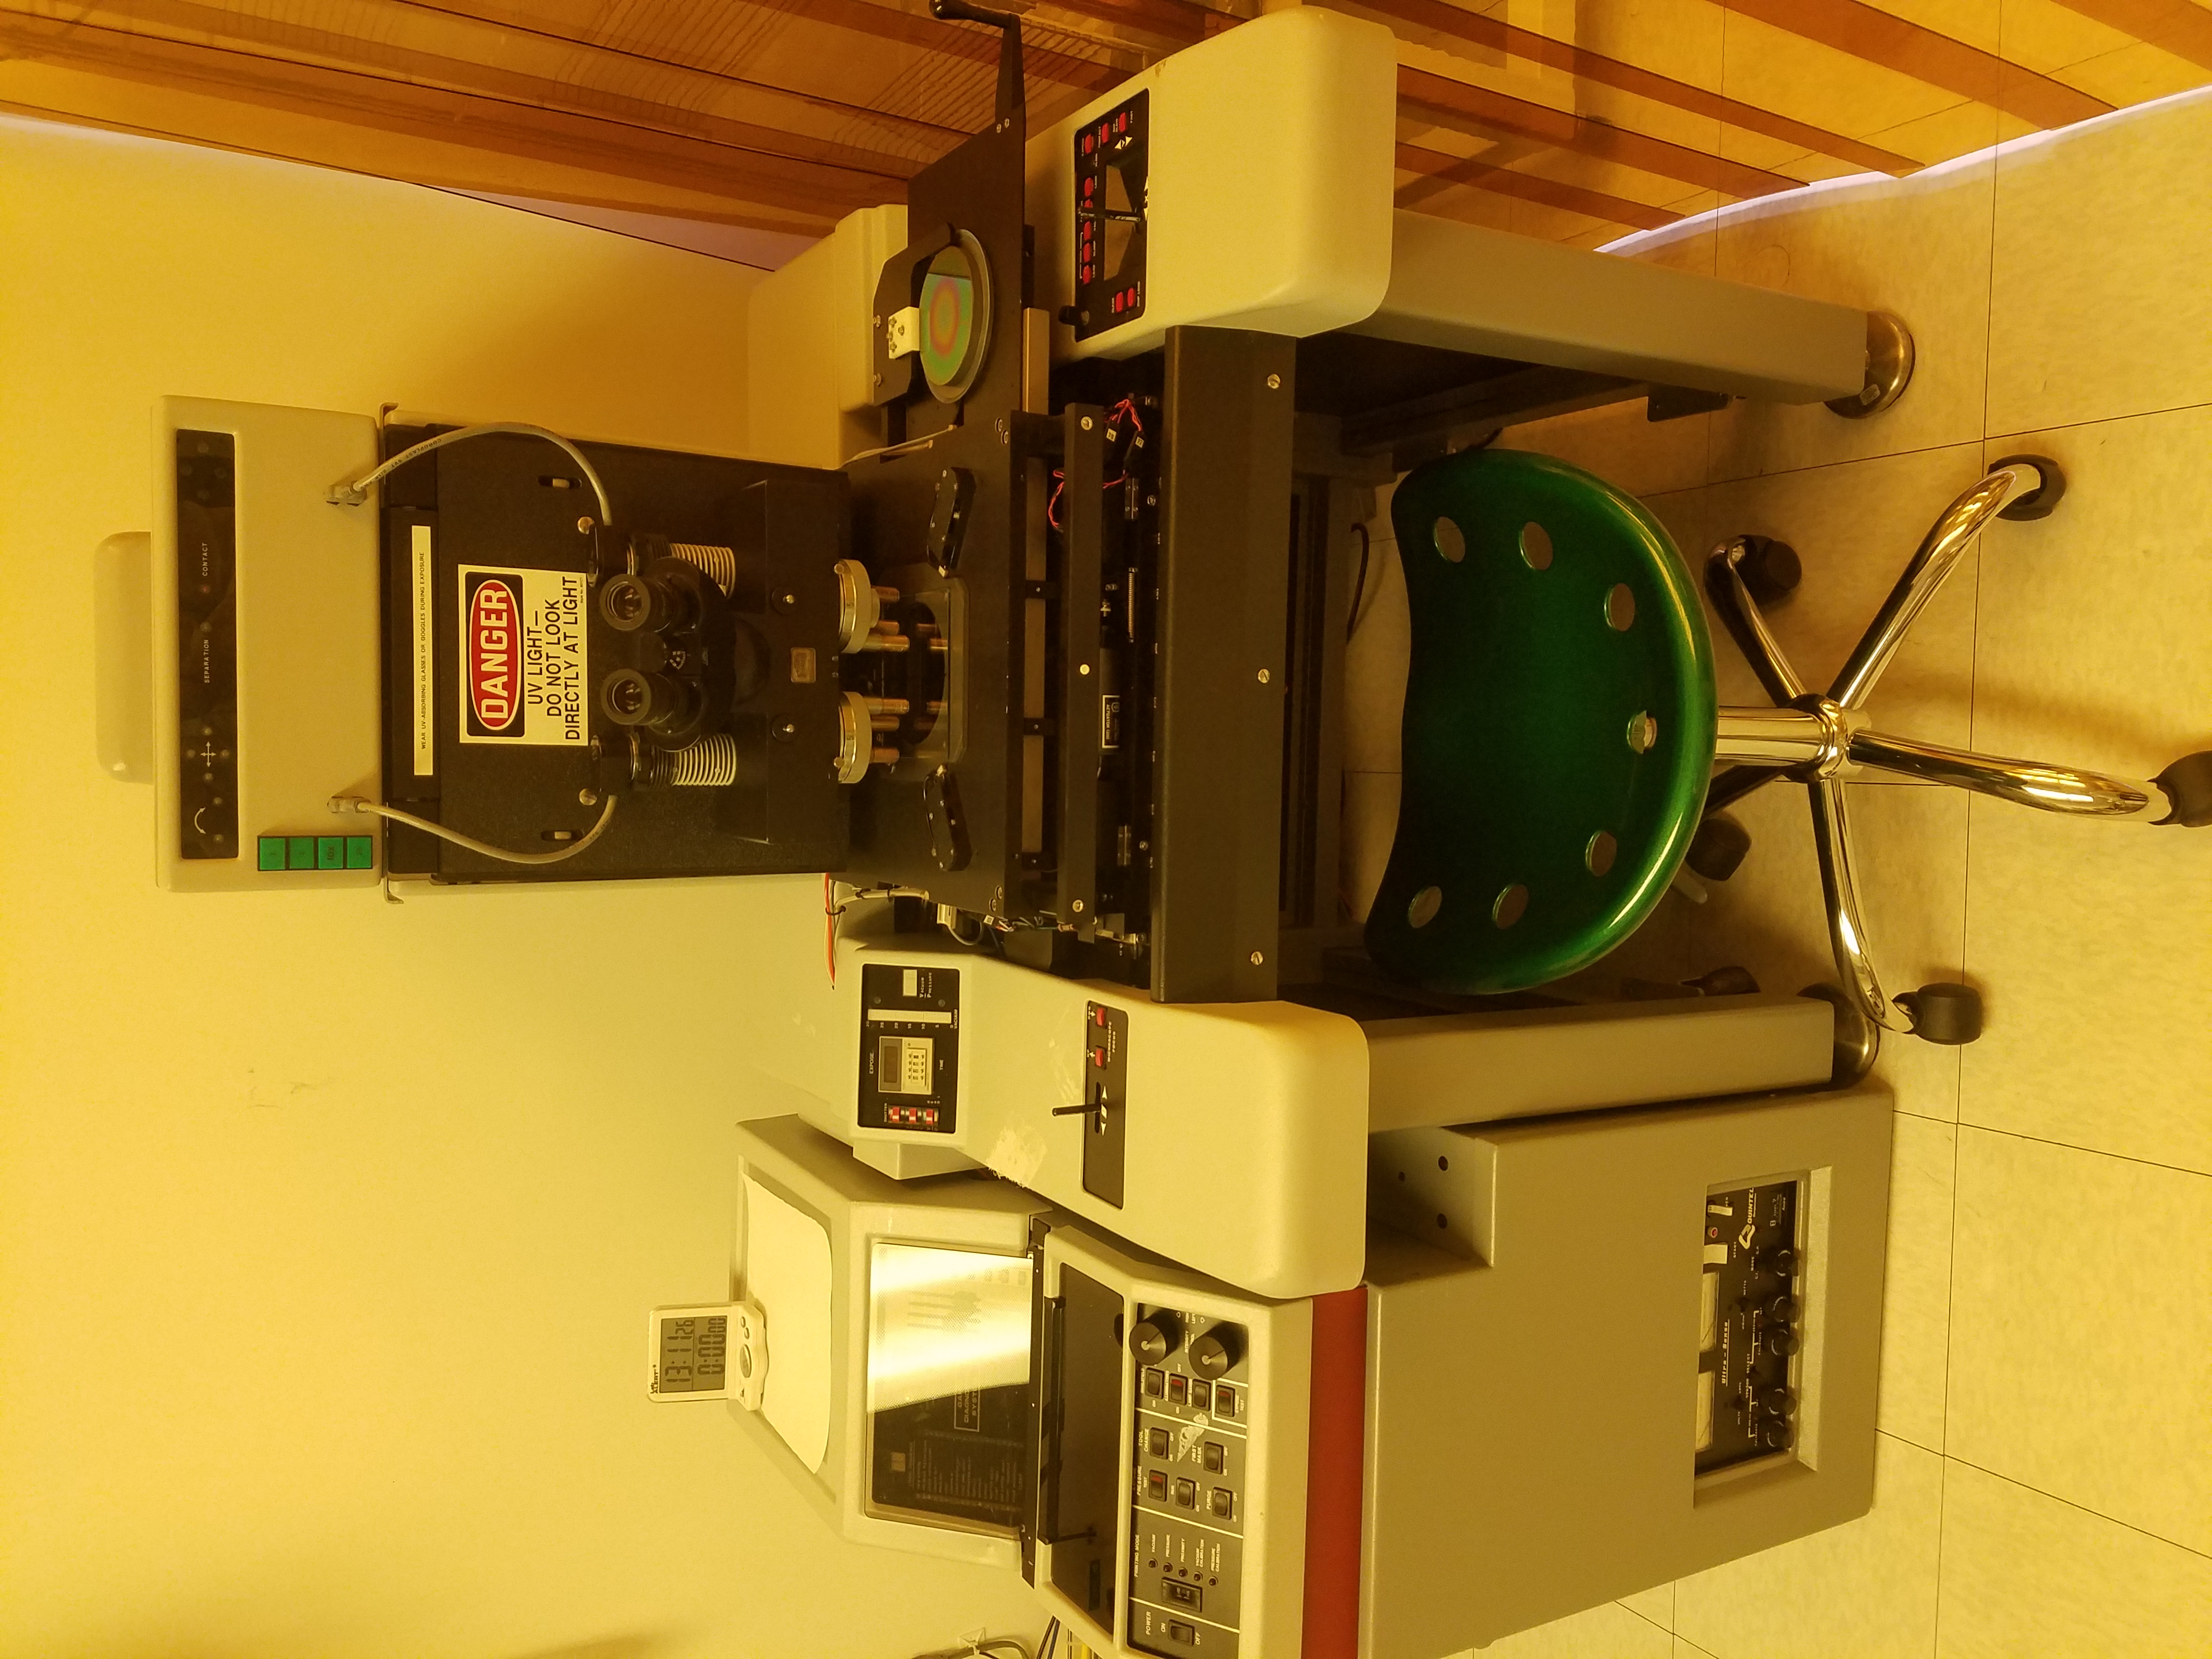
\includegraphics[width=0.7\textwidth]{images/aligner.jpg}
    \caption{Cannon PLA501FA mask aligner}
    \label{fig:mask_aligner}
\end{figure}

\par The photolithography process was completed using the Cannon PLA-501FA mask aligner (figure \ref{fig:mask_aligner}). With the transparency mask centered over the wafer and the 365 nm glass-transparency filter in place, UV light was applied to the photoresist for 14 seconds with a total exposure of 140 mJ/cm$^2$. The wafer was then baked at 85 $^\circ$C for 4 minutes with a 10 minute cool down. 

\par The wafer was then developed in propylene glycol monomethyl ether acetate (SU-8 developer, MicroChem) in order to remove the non-exposed SU-8 from the wafer. The wafer was placed in the SU-8 developer for 3 minutes. The wafer was then hard baked for 15 minutes at 210 $^\circ$C. 

The detailed procedure steps are provided in appendix \ref{app: su-8_photolith}.

\subsection*{Soft Lithography}
\par The polydimethylsiloxane (PDMS) for soft lithography was obtained by purchasing a Dow Corning 184 Sylgard kit through Ellsworth adhesives. The kit comes with a base and a curing agent that cross links the PDMS and increases the polymer's stiffness. The PDMS was prepared by mixing the base and the curing agent with a 10:1 ration. The mixture was then degassed under vacuum until the PDMS was clear and free of bubbles (figure \ref{fig:pdms_vacuum}). The PDMS was then poured directly onto the SU-8 master mold until the PDMS covered the wafer with approximately 1/4" depth. The PDMS was cured by baking in an oven for at least an hour at 65 $^\circ$. The PDMS chips were cut from the master mold with a scapel and peeled off the wafer. 

\begin{figure}[h]
    \centering
    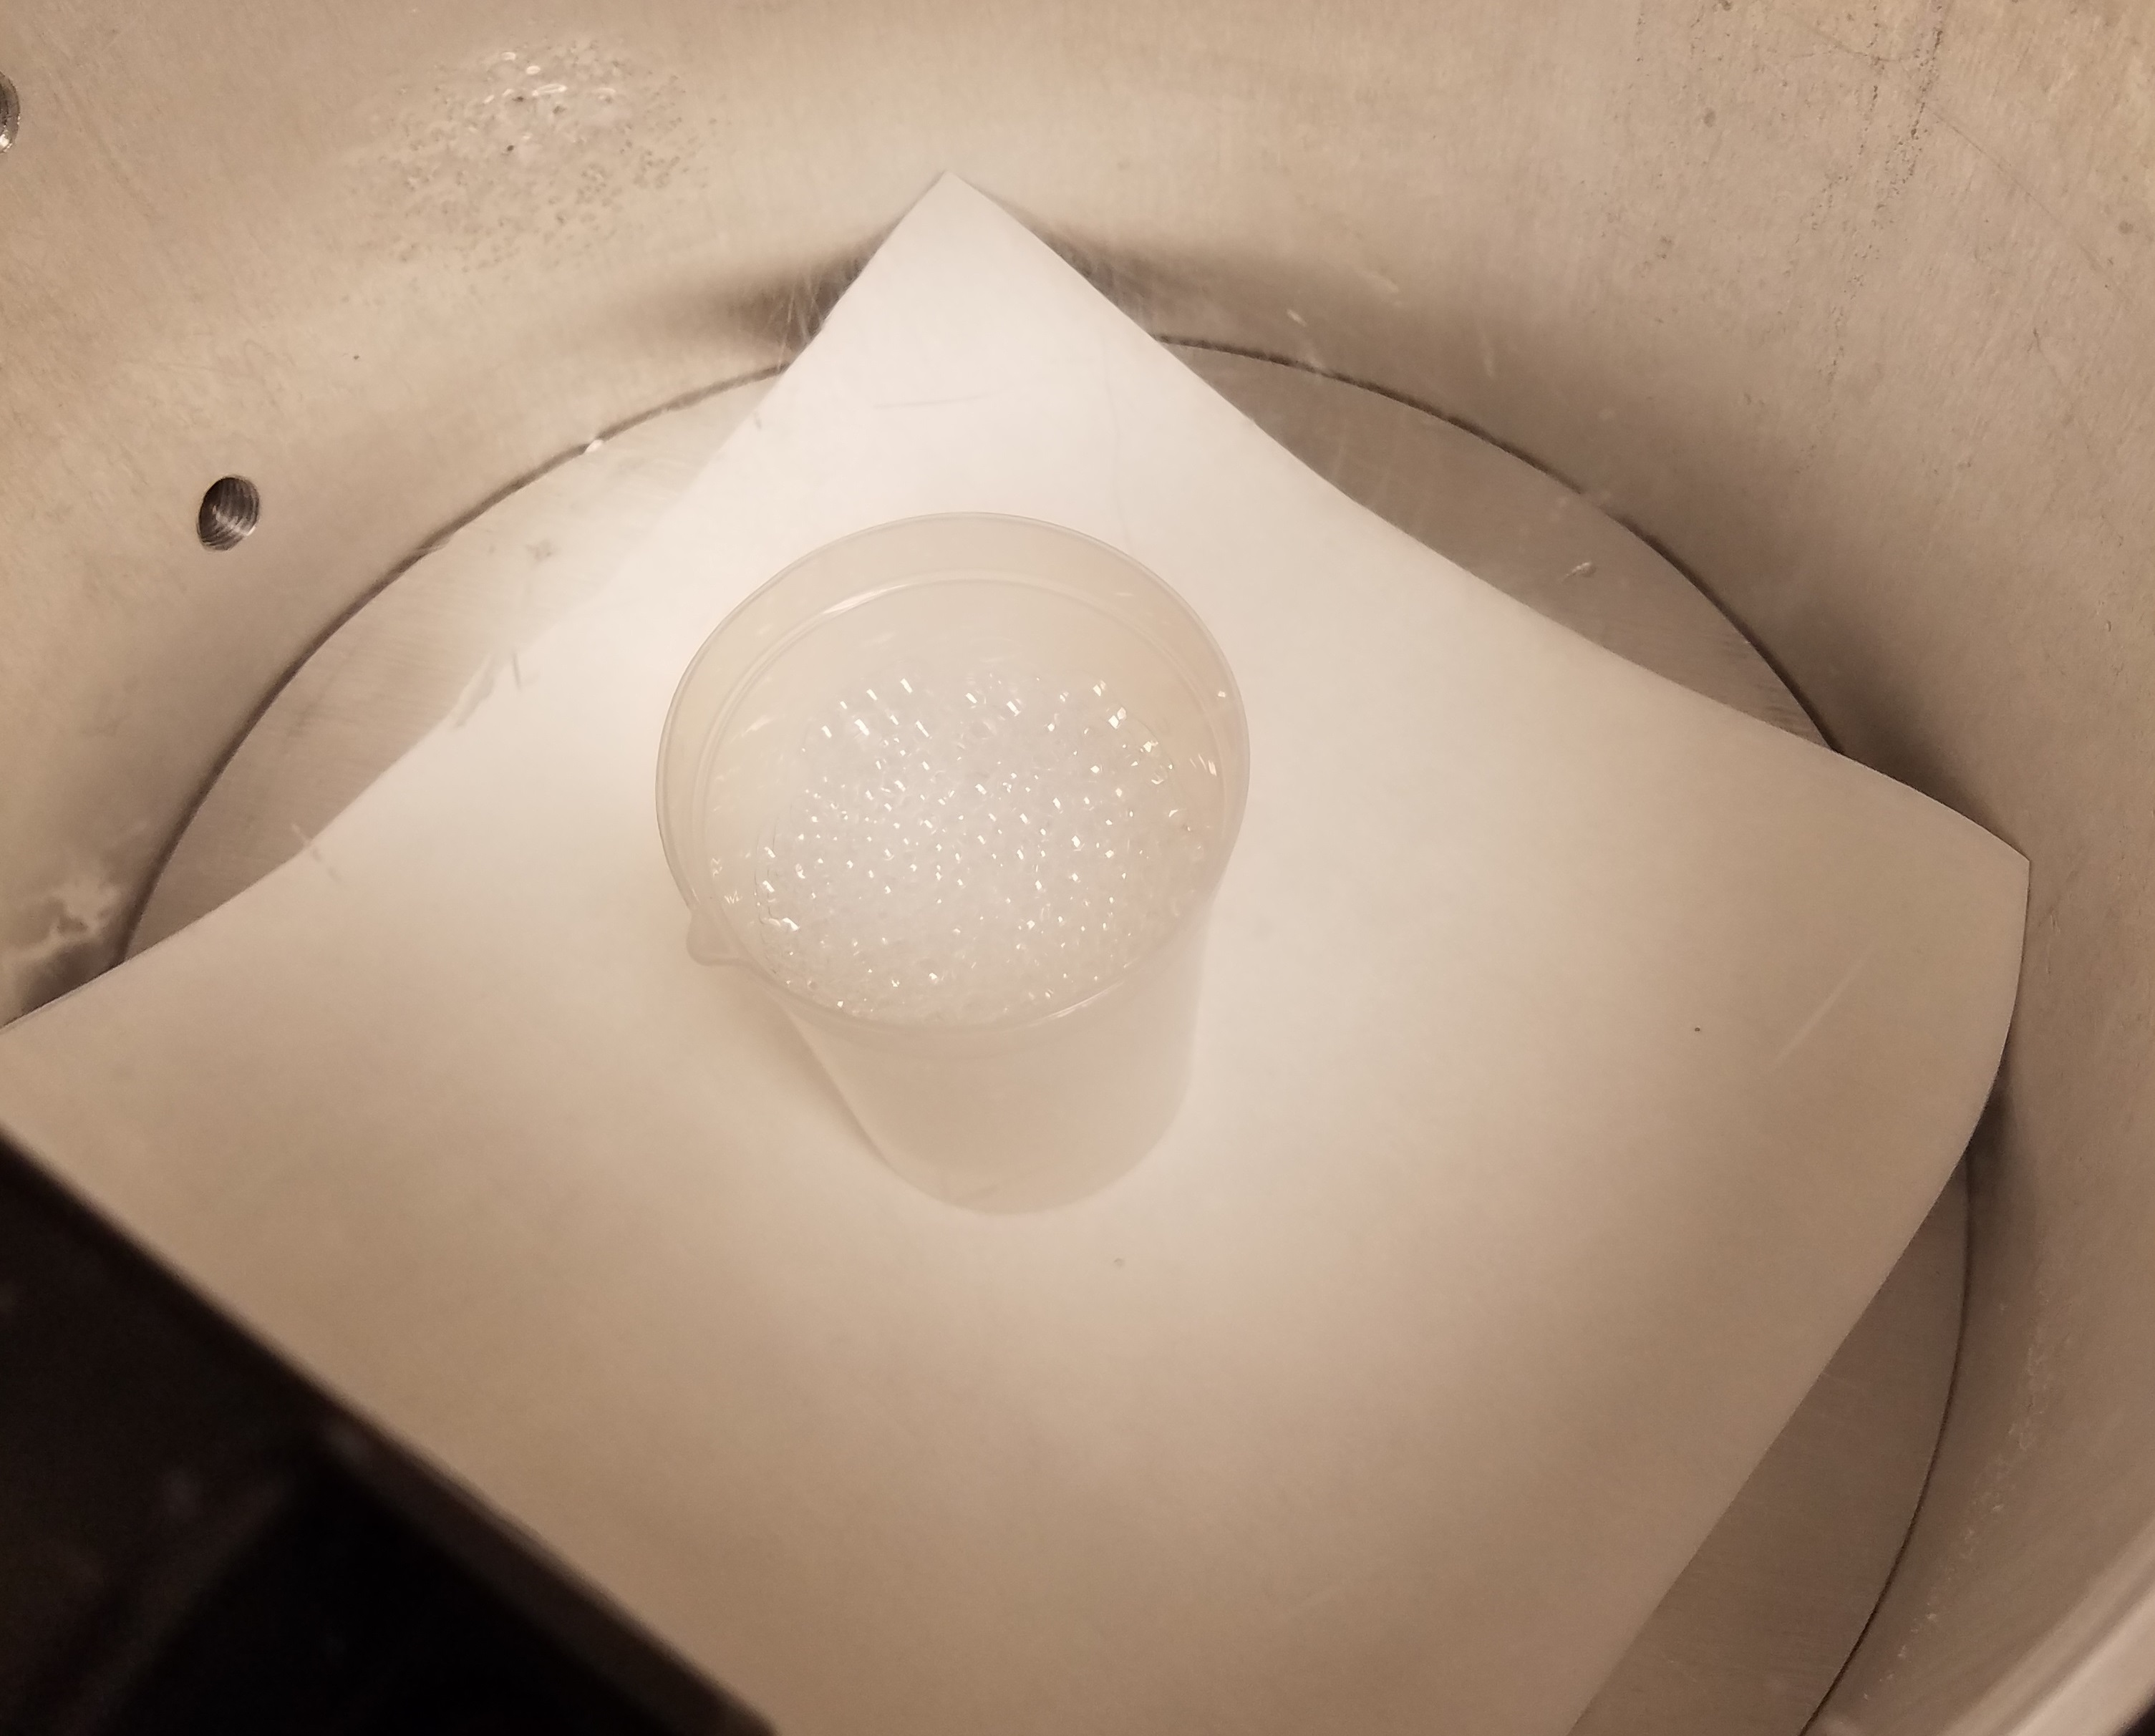
\includegraphics[width=0.65\textwidth]{images/pdms_in_vacuum.jpg}
    \caption{Degassing PDMS mixture under vacuum.}
    \label{fig:pdms_vacuum}
\end{figure}


\par The finished product was a PDMS chip with the desired microchannel dimensions molded into the polymer surface. The procedure steps for soft lithography are provided in appendix \ref{app: soft_litho}.


\subsection{Electrode Fabrication}

\par The device electrodes were fabricated onto a glass substrate using the lift-off process (section \ref{sec: lift_off}). The process utilized a 6"x6", 20,000 DPI transparency mask ordered from CAD/art services Inc. A flow chart of the overall process is depicted in figure \ref{fig:lift_off}.

\subsection*{Photolithography}

\par Glass wafers were prepared for the lift-off process by cleaning the wafers in a pirahna bath (pirahna def??) for 15 minutes and rinsing in DI water, and then a 1 minute dip in BOE (BOE definition???) and rinsing in DI before running the wafers through the SRD (SRD definition???). The wafers were then dehydrated by baking on a hot plate for 10 minutes at 200 $^\circ$C and then allowed to cool down fro five minutes. 

\begin{figure}[h]
    \centering
    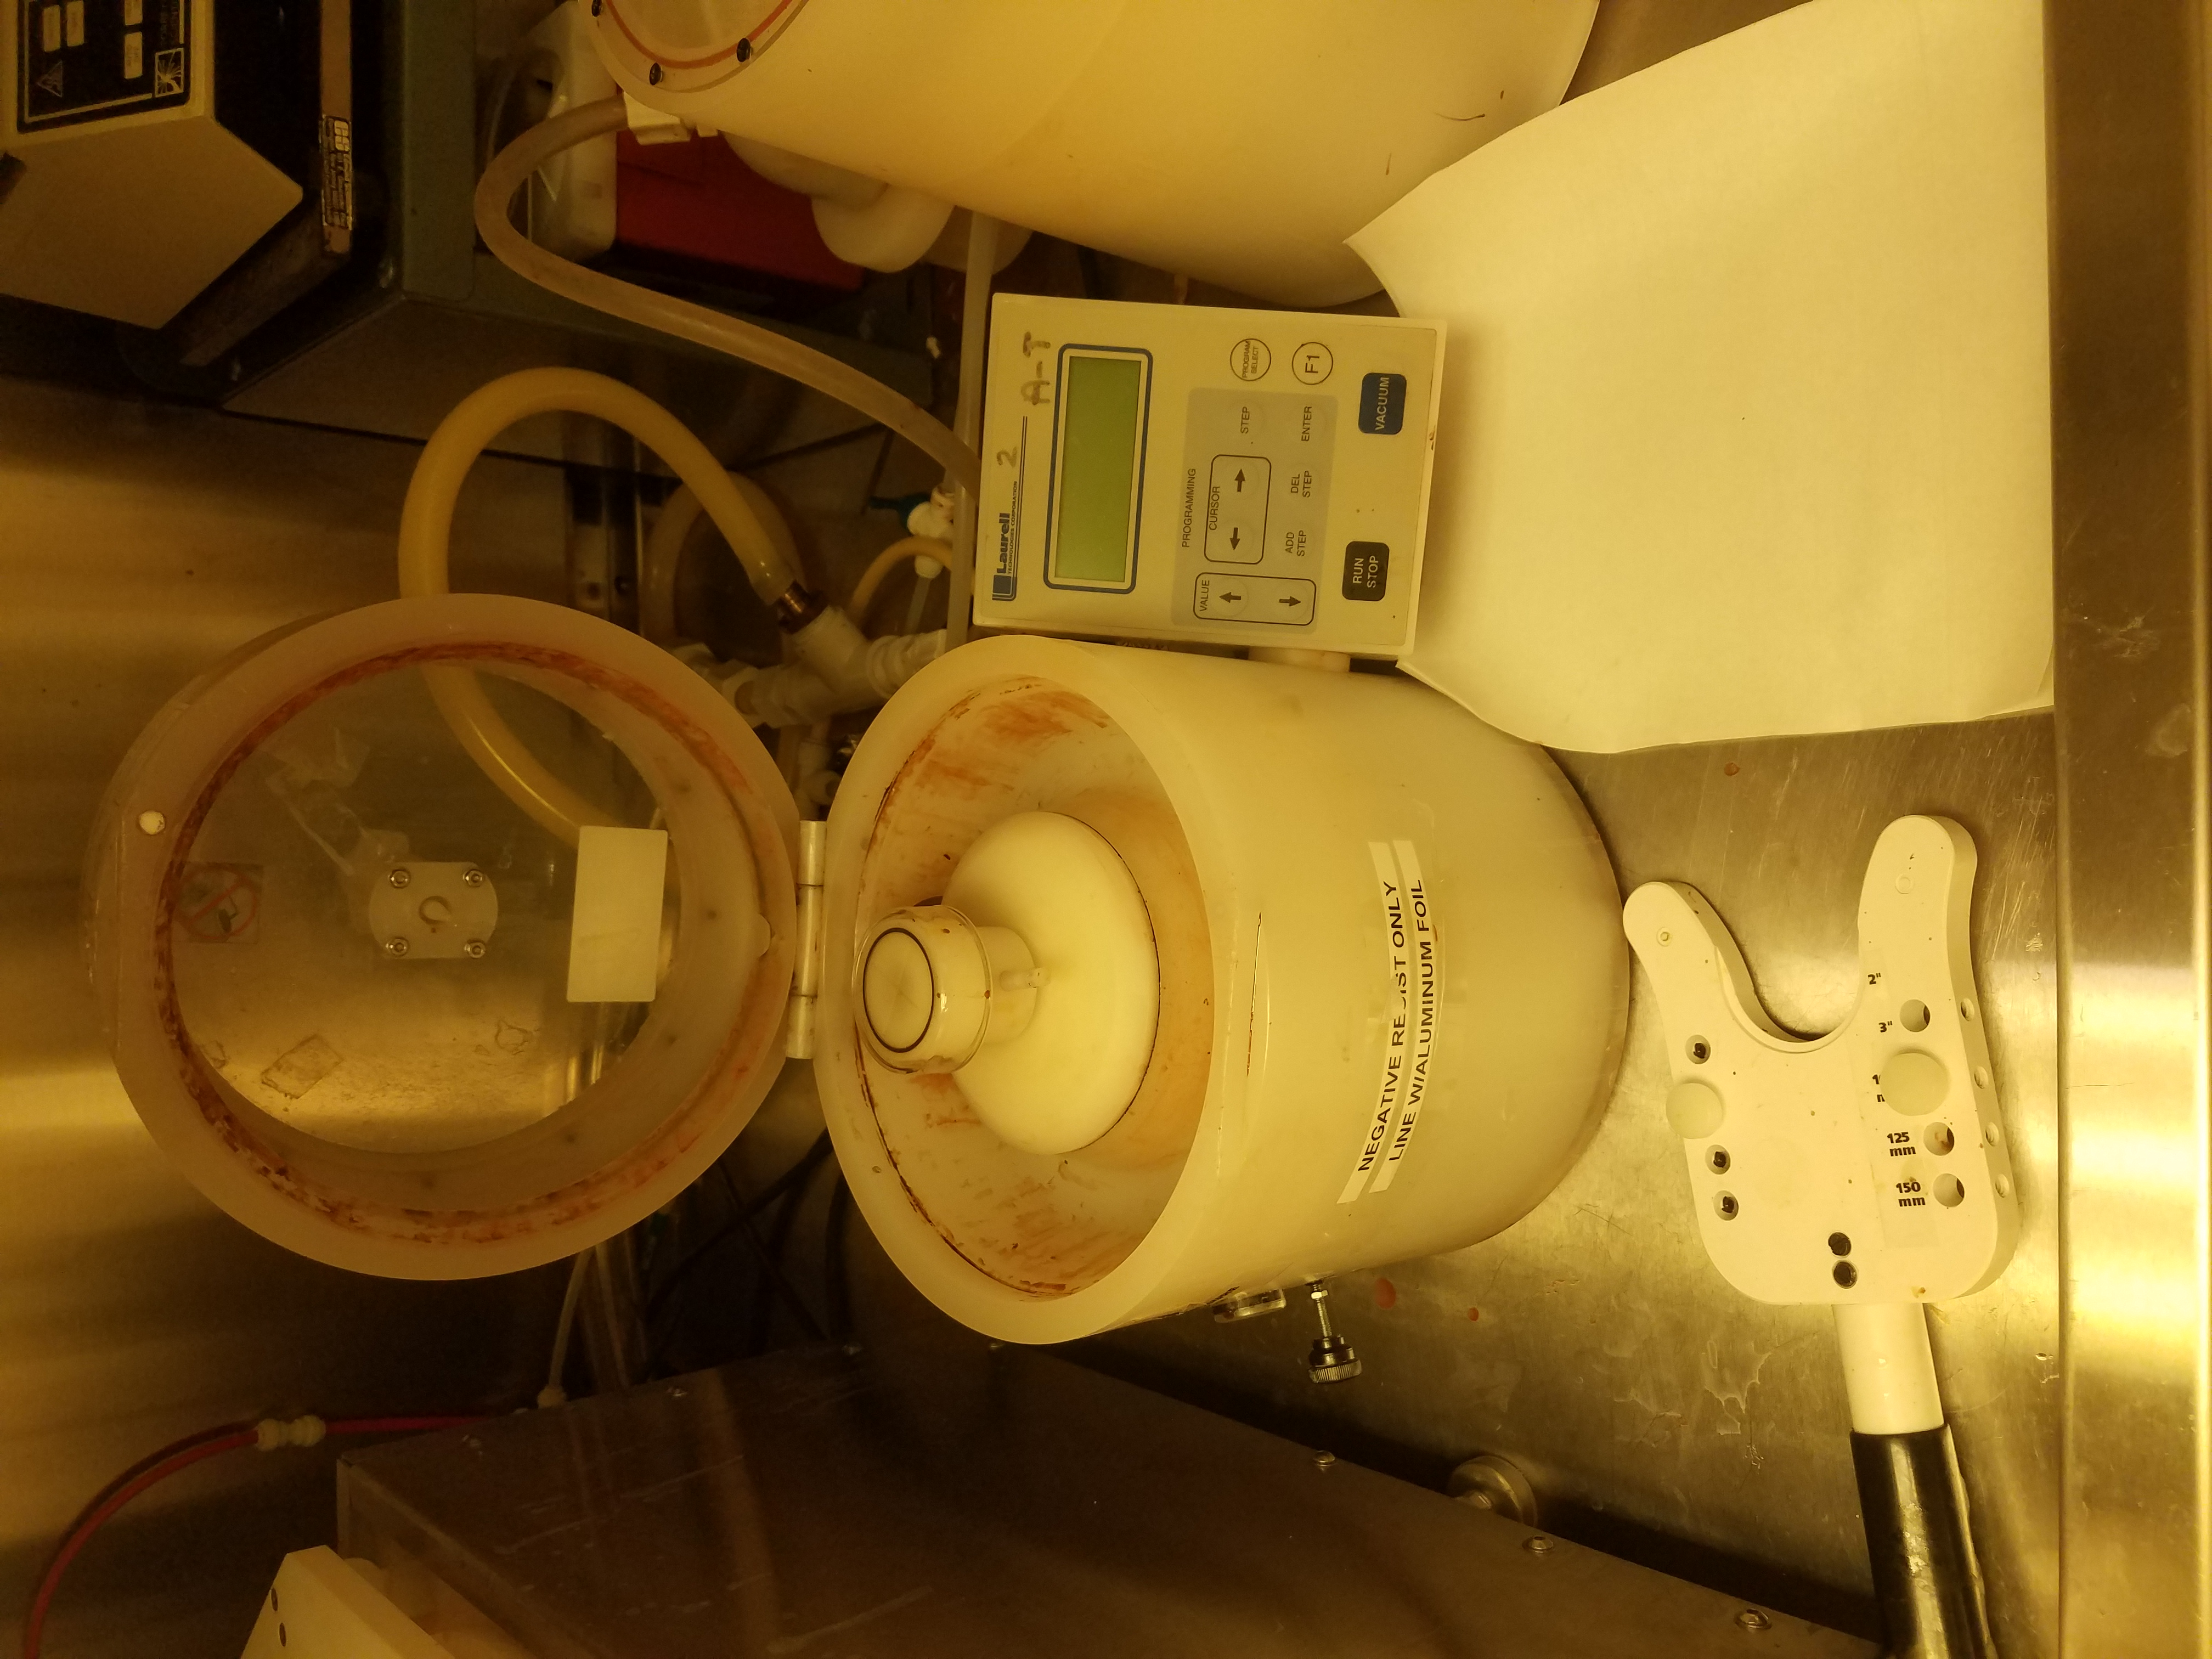
\includegraphics[width=0.8\textwidth]{images/resist_spinner_open.jpg}
    \caption{Laurel technologies ws-400 spin coater}
    \label{fig:spin_coater}
\end{figure}

\par The wafers were coated with ma-N1420 negative-tone photoresist on a spin coater (Laurel technologies, ws-400; \ref{fig:spin_coater}). The ma-N1420 photoresist is advantageous for the lift-off process since the developed photoresist has an undercut profile and the cross-linked photoresist is durable in contrast to the "soft" positive photoresist. Before application of the ma-N1420 a primer (primer definition???) is dispersed and then spun onto the wafer at 3000 RPM for 30??? seconds. Ma-N1420 is then dispersed onto the glass wafer, but before spinning, ensure that the photoresist spreads to all edges of the wafer. The photoresist was spun at 2000 RPM for 35??? seconds with a target of 2.5 micron thickness. The wafers were then soft-baked on a hotplate at 120 $^\circ$C for 3 minutes to increase stability. 

\par The photolithography process was completed using the Cannon PLA-501FA mask aligner (figure \ref{fig:mask_aligner}). The glass wafer was placed in the aligner with a black tape backing in order to prevent light scattering and absorb radiation, and the transparency was centered over the wafer. UV light was applied to the wafer for 30 seconds for a total of 450 mJ/cm$^2$. 

\par The wafer was then developed for 60-90 seconds in something?? based developer (ma-D 533/3) and then rinsed in DI water. At this step, it is critical to examine the wafer under a microscope to ensure the photoresist is entirely removed from the substrate where the electrode is desired and that the electrode edges are sharp. If not, develop for another 10 seconds and reexamine. 

\par After the photoresist is fully developed, the wafer was flood-exposed (i.e. no transparency) in order to improve stability. The photoresist was exposed 3 times for 40 seconds with a five minute rest between each exposure for a total of 1800 mJ/cm$^2$ of exposure. Finally, the wafers were baked on the hotplate with a ramping temperature from 60 $^\circ$C to 100 $^\circ$C for 10 minutes, and then allowed to cool for 10 minutes. 

\subsection*{Metal Deposition}

\par To deposit the electrode metals onto the developed-photoresist wafer, the AGS reactive ion etcher, CrC-150 chrome sputterer, and the Denton Desk V sputtering system were used to clean and sputter chromium and gold. The target metal deposition consists of three layers: a 125 \si{\angstrom} thick base chromium layer to facilitate adhesion of the electrode to glass, a 180 nm thick gold layer as the main conductor in the electrode, and a 42 \si{\angstrom} thick layer of chromium that will oxidize to an inert finish (figure \ref{fig:metal_deposition}).

\begin{figure}[h]
    \centering
    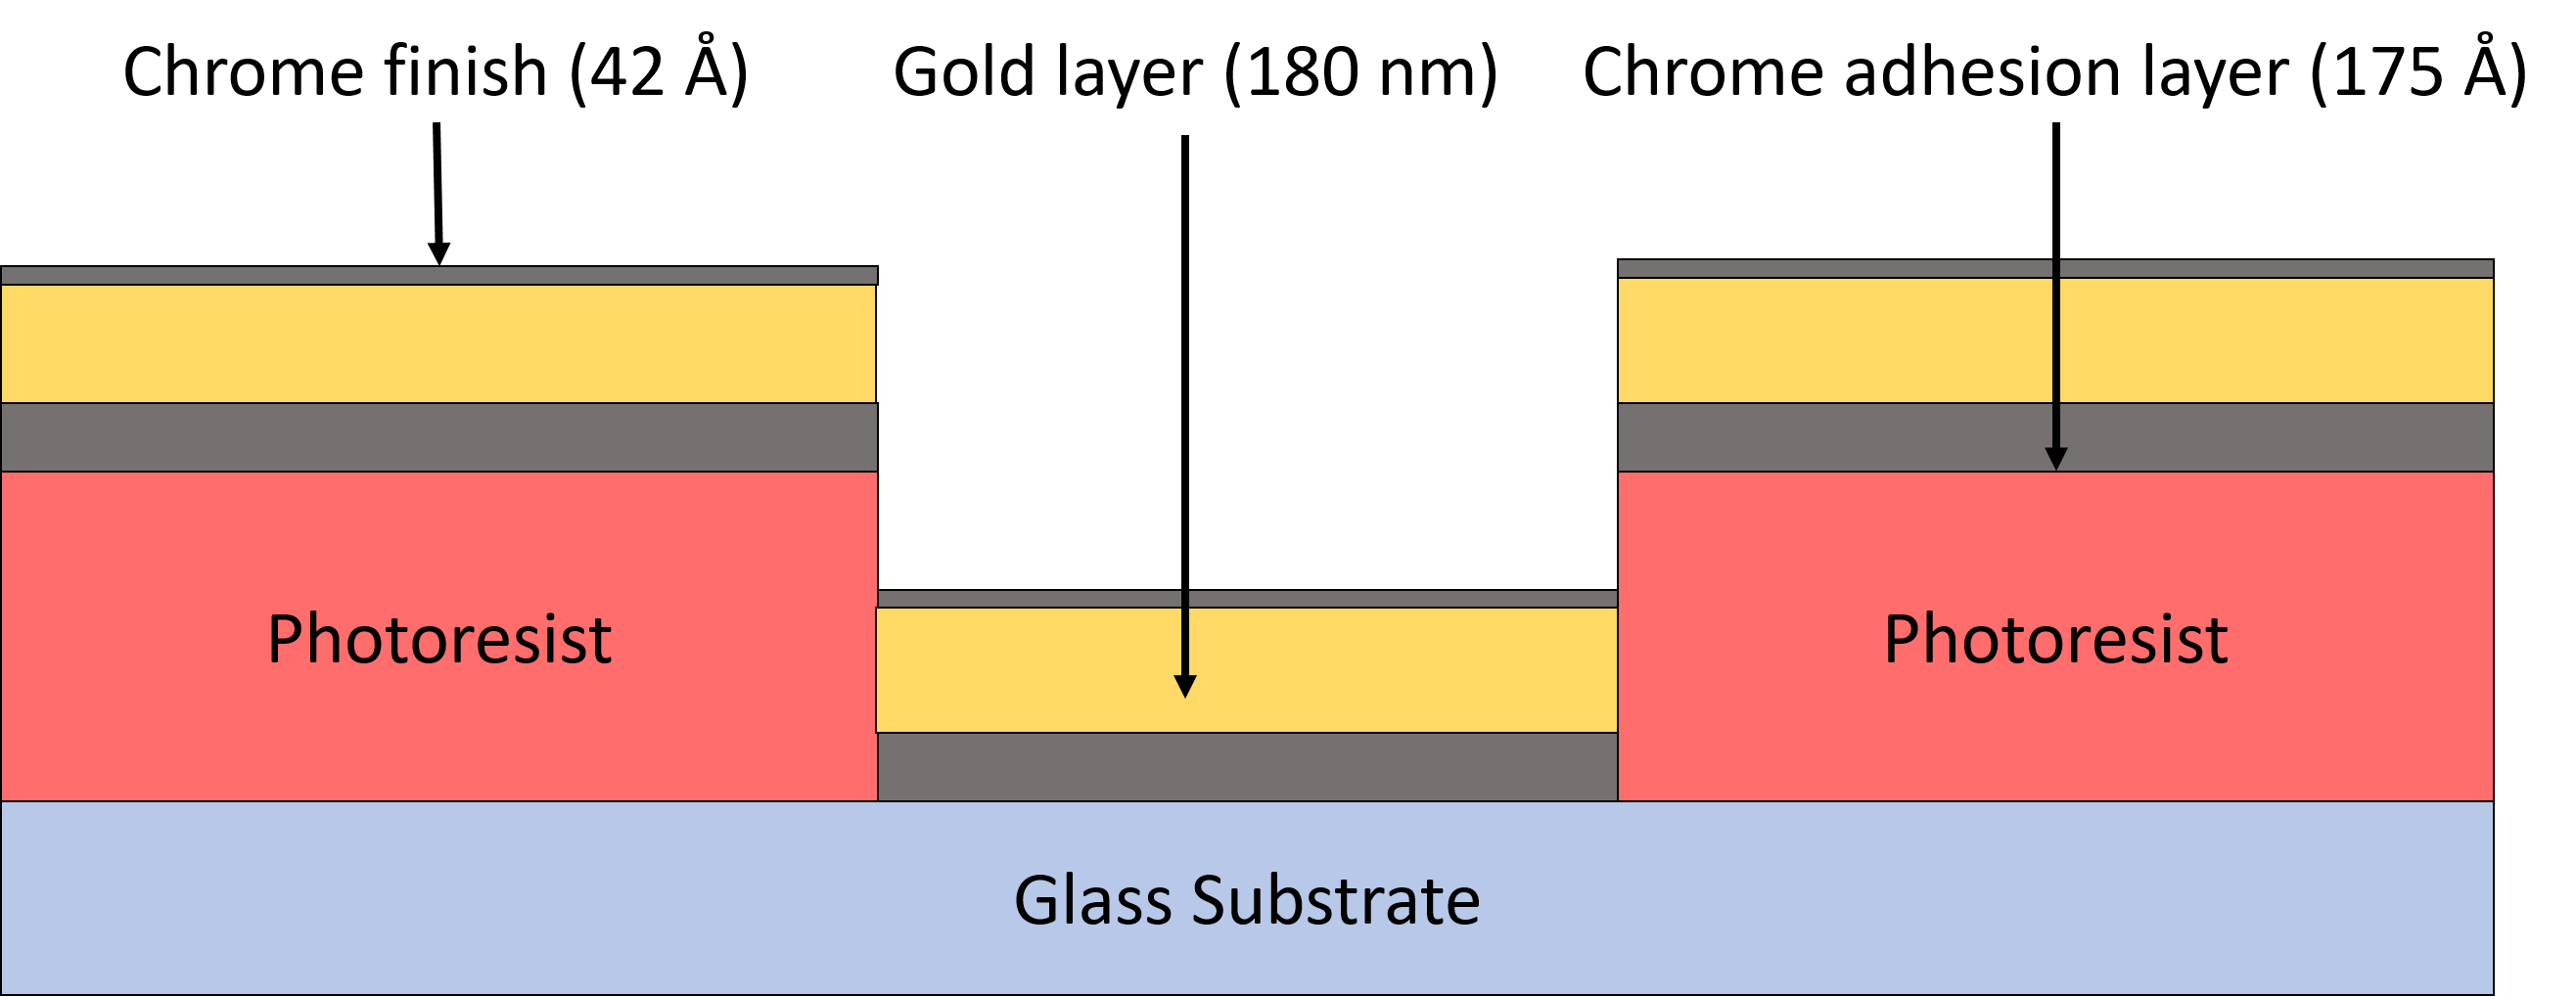
\includegraphics[width=\textwidth]{images/metal_deposition_diagram.png}
    \caption[Diagram of metal deposition onto photoresist-developed substrate]{Diagram of the three layered metal deposition onto photoresist-developed substrate.}
    \label{fig:metal_deposition}
\end{figure}

\par To prepare the photoresist-developed wafer for metal deposition, the wafers were exposed to an oxygen plasma to volatilize and remove organic residues. The wafer was placed under vacuum in the AGS RIE system and exposed to an oxygen plasma for 30 seconds (figure \ref{fig:AGS-RIE}). The CrC-150 sputtering system was then used to deposit 125 \si{\angstrom} of chromium at a rate of 250 \si{\angstrom} per minute for 30 seconds. Using the Denton Desk 5, 180 nm of gold was deposited at a rate of 180 \si{\angstrom} per minute for 10 minutes. A final 42 \si{\angstrom} layer of chromium was deposited with the CrC-150 with a rate of 250 \si{\angstrom} per minute for 10 seconds (figure \ref{fig:sputterers}). 

\begin{figure}
    \centering
    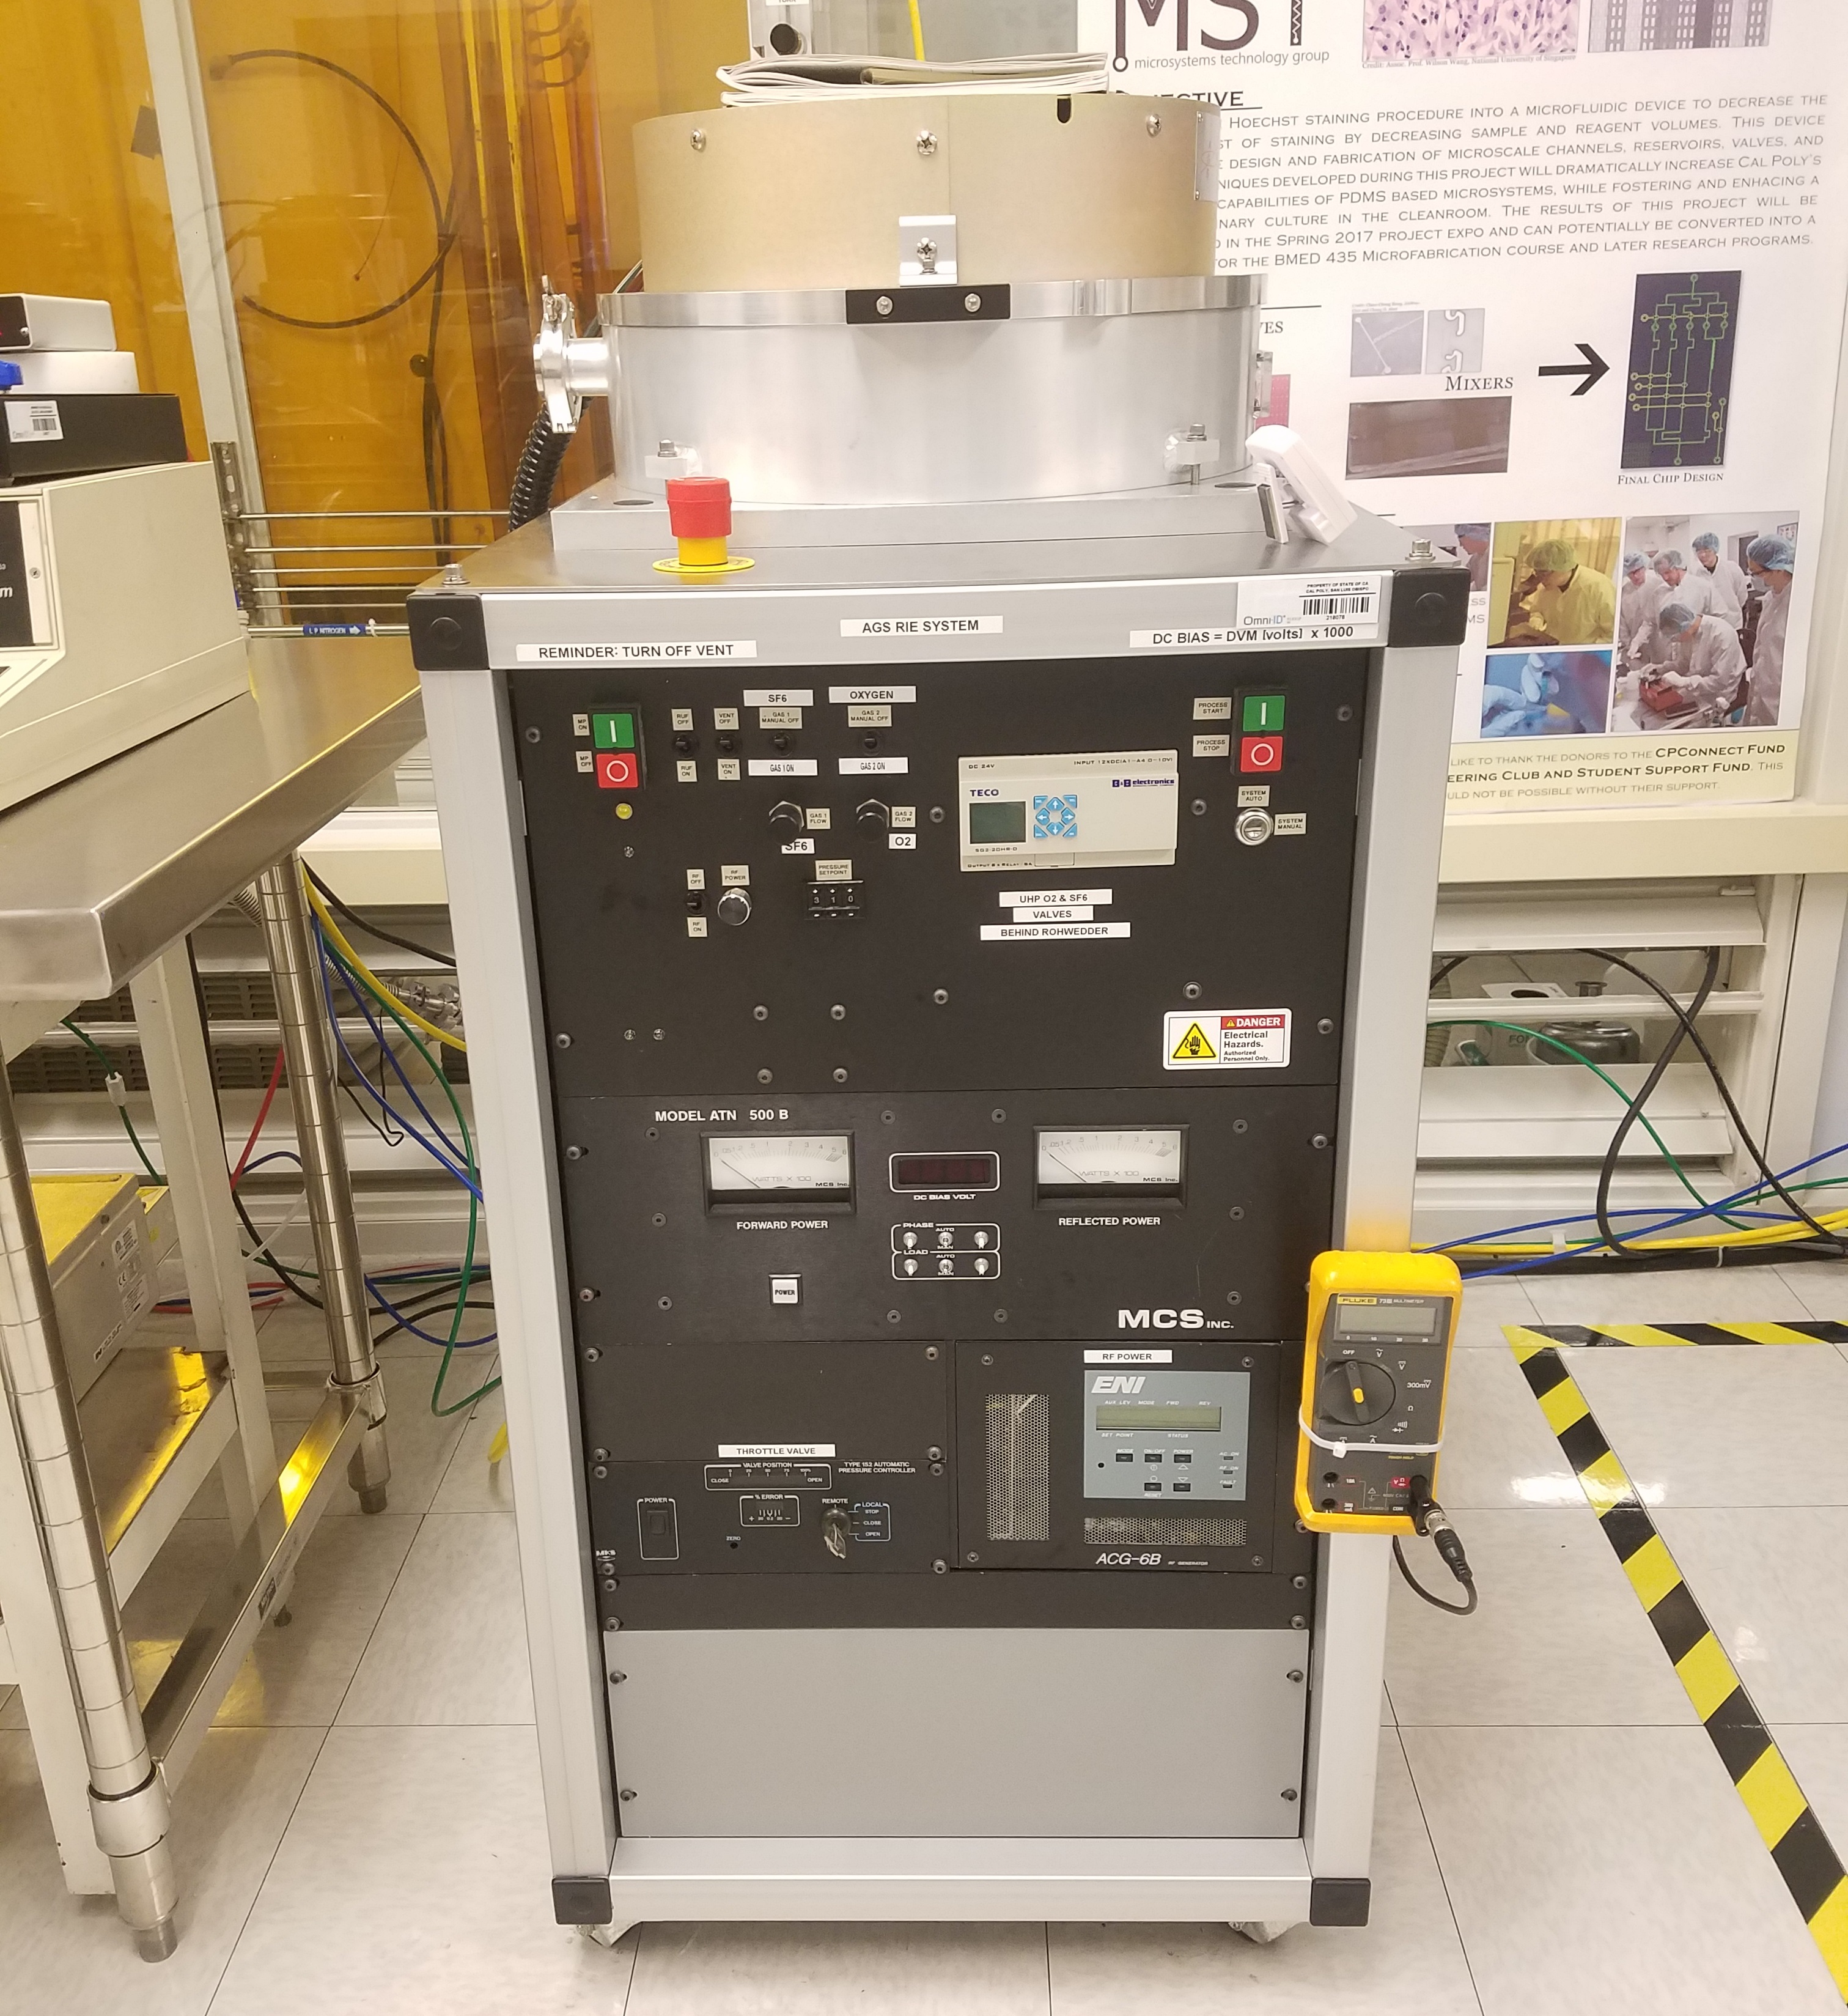
\includegraphics[width=0.7\textwidth]{images/AGS_RIE.jpg}
    \caption[AGS reactive ion etcher]{The AGS reactive ion etcher used to remove organic residue with an oxygen plasma.}
    \label{fig:AGS-RIE}
\end{figure}

  \begin{figure}[h]
    \centering
    \begin{subfigure}[b]{0.45\textwidth}
        \centering
        \includegraphics[width=\textwidth]{images/CrC-150.jpg}
        \caption{CCr-150 Sputter system}
        \label{fig:ccr-150}
    \end{subfigure}
    \hfill
    \begin{subfigure}[b]{0.45\textwidth}
        \centering
        \includegraphics[width=\textwidth]{images/denton.jpg}
        \caption{Denton Desk V Sputter/Etch unit}
        \label{fig:denton}
    \end{subfigure} 
    \caption[Sputter machines used for metal deposition]{The sputter machines used for metal deposition. The CCr-150 and the Denton Desk V were used for chromium and gold deposition respectively.}
    \label{fig:sputterers}
 \end{figure}

\par During the transition between sputtering systems, the wafers were kept under vacuum in order to keep them clean, and in the case for chromium depositions, to reduce the formation of chromium oxide which can significantly impair chromium-gold adhesion.

\subsection*{Lift Off}

The final step of the electrode fabrication process was to remove the photoresist with the undesired metal depositions. The wafers were submerged in Microposit remover 1165 for five days under constant agitation (figure \ref{fig:lift_solution}). To increase the speed of lift off, the solution can be heated to 65$^\circ$C.

\begin{figure}
    \centering
    \begin{subfigure}[b]{0.45\textwidth}
        \includegraphics[width=\textwidth]{images/lift_off.jpg}
        \caption{Sputtered wafer in Microposit remover}
        \label{fig:lift_solution}
    \end{subfigure}
    \hfill
    \begin{subfigure}[b]{0.45\textwidth}
        \centering
        \includegraphics[width=\textwidth]{images/electrodes.jpg}
        \caption{Wafer with electrode post lift off}
        \label{fig:electrode_methods}
    \end{subfigure} 
    \caption[Lift off]{The lift off process with metal depositions removed from the glass substrate with Microposit remover 1165 in (a) and the remaining depositions after the lift off process in (b).}
    \label{fig:electrode_methods}
\end{figure}

\subsection{Device Assembly: Alignment and Plasma Bonding}

\par To assemble the PDMS chip containing the microfluidic channels to the electrodes on the glass substrate, the components were plasma bonded to create a water-tight seal that permits optical viewing. The PDMS and the galss electrode substrate were placed device-side up in the Cal Poly Microfabrication Lab's PDC-32G plasma cleaner. After pumping the plasma cleaner down to a vacuum, the device was exposed to an atmospheric plasma for 10 seconds.  

\begin{figure}
    \centering
    \includegraphics[width=\textwidth]{images/plasma_cleaner.jpg}
    \caption[PDC-32G plasma cleaner]{PDC-32G plasma cleaner used for plasma bonding.}
    \label{fig:my_label}
\end{figure}

\par After plasma activation, a drop of ethanol was place don the PDMS surface before placing the PDMS onto the electrode substrate in order to create a liquid float barrier to that will prevent permanent binding for $\sim$5 minutes. The electrodes and PDMS microchannels were aligned by hand with a microscope set at 20X magnification for visual feedback. After proper alignment, the device was baked in an oven at 65$^\circ$C for an hour. 



\section[Software]{Software Interface}

\par LabVIEW was used to interface with the NI-5421 function generator and the NI-5124 oscilloscope to package the circuit model, data acquisition, and data analysis into an impedance spectroscope program. The LabVIEW language was chosen due to the ease of connecting to the National Instrument hardware and the rapid development cycle. The program specifications include interfacing with the NI-hardware to run an impedance spectroscopy experiment, the ability to control the sweeping frequencies, the ability to switch circuit topologies, the ability to automatically run tests at specified intervals, the implementation of a data saving system that records the users settings for the experiment as well as the impedance spectroscopy results, and the ability to view and compare data.

\begin{figure}[h]
    \centering
    \begin{subfigure}[b]{\textwidth}
        \centering
        \includegraphics[width=0.85\textwidth]{images/program_overview.png}
        \caption{Event-driven state machine architecture}
        \label{fig:IS_architecture}
    \end{subfigure}
    \vspace{0.1 in}
    \vfill
    \begin{subfigure}[b]{\textwidth}
        \centering
        \includegraphics[width=\textwidth]{images/event_driven_SM.png}
        \caption{Event-driven state machine code setup}
        \label{fig:IS-base_code}
    \end{subfigure}
    \caption[Event-driven state machine architecture]{The event-driven state machine architecture used for the impedance spectroscope LabVIEW program. Events override the state of the state machine that runs inside the time out event.}
    \label{fig:IS_software_design}
\end{figure}
\FloatBarrier

\subsection{Architecture}

\par The LabVIEW program was designed with an event-driven state machine architecture and is diagrammed in figure \ref{fig:IS_software_design}. A state machine is a common LabVIEW coding pattern where the program exists as a set of states. Depending on user input or calculations, each state leads to a subsequent state that can potentially lead to a large network of modular decision making states. For the impedance spectroscope, the state machine is simple with most states leading to an idle state that continues to wait for user input. The state machine lives inside an event structure that listens for specific user interface (UI) interactions that triggers an event that runs code and can specify the next state in the state machine. After a specified amount of time passes without an event triggering, the time out event will trigger and run the state machine.    

\par The event driven state machine architecture will allow for a responsive UI that can adapt outside of the state machine architecture while maintaining the modularity of a state machine with safe program initialization and exit. The implementation of the software resulted in two main functions: impedance spectroscopy, and the data viewer.

\subsection{Impedance Spectroscopy}
\par The impedance spectroscopy UI gives users the ability to set settings for experiments and view the results (figure \ref{fig:is_gui}). All of the gui settings are located in a set of three tabs: circuit topology, frequency parameters, and interval parameters. 

\begin{figure}[h]
    \centering
    \includegraphics[width=\textwidth]{images/IS_gui.png}
    \caption{Impedance spectroscopy user interface}
    \label{fig:is_gui}
\end{figure}

\par The circuit topology tab tell the software what circuit is being used and the value of the external resistor (figure \ref{fig:labview_circuit_settings}). With each circuit selection, an image below updates to display where the software expects the oscilloscope channels to be connected and the formula calculating impedance. In the current implementation, the software includes options for the I-V and auto-balancing bridge circuits. 


\begin{figure}[h]
    \centering
    \begin{subfigure}[b]{0.48\textwidth}
        \centering
        \includegraphics[width=\textwidth]{images/labview_circuit_IV.png}
        \caption{I-V topology}
        \label{fig:labview_I-V_circ}
    \end{subfigure}
    \hfill
    \begin{subfigure}[b]{0.48\textwidth}
        \centering
        \includegraphics[width=\textwidth]{images/labview_circuit_auto.png}
        \caption{Auto-balancing bridge topology}
        \label{fig:labview_auto_circ}
    \end{subfigure}
    \caption{Circuit settings}
    \label{fig:labview_circuit_settings}
\end{figure}

\par The frequency parameter tab contains the controls that determine what frequencies are swept over in the impedance spectroscopy experiment (figure \ref{fig:labview_frequency_settings}). The frequency expression shows how frequency values are calculated with x and y representing incremented values with the caveat that a value for every increment of x is generated for every one increment of y. For example, with the settings given in figure \ref{fig:labview_frequency_settings}, ten frequencies per decade with decades 1E3 to 1E7 are generated. The max input frequency truncates the frequencies generated to the specified value. In addition to frequency parameters, the tab also includes controls for the waveform amplitude, the number of cycles measured by the oscilloscope and the sample rate. 

\begin{figure}[h]
\centering
\begin{minipage}[t]{.48\textwidth}
  \centering
  \includegraphics[width=\textwidth]{images/labview_freq.png}
  \captionof{figure}{Frequency sweep options}
  \label{fig:labview_frequency_settings}
\end{minipage}
\vspace{0.2 in}
\vfill
\begin{minipage}[t]{.48\textwidth}
  \centering
  \includegraphics[width=\textwidth]{images/labview_intervals.png}
  \captionof{figure}{Interval measurement settings}
  \label{fig:labview_interval_settings}
\end{minipage}
\end{figure}

\par The interval parameters tab contains options for running automatic experiments at timed intervals (figure \ref{fig:labview_interval_settings}). 

\begin{figure}[h]
    \centering
    \begin{subfigure}[b]{0.48\textwidth}
        \centering
        \includegraphics[width=\textwidth]{images/labview_mag_phase_graph.png}
        \caption{Impedance magnitude and phase}
        \label{fig:labview_mag-phase_graph}
    \end{subfigure}
    \hfill
    \begin{subfigure}[b]{0.48\textwidth}
        \centering
        \includegraphics[width=\textwidth]{images/labview_real_imag_graph.png}
        \caption{Real and imaginary impedance graphs}
        \label{fig:labview_real-imag_graph}
    \end{subfigure}
    \vspace{0.2in}
    \vfill
    \begin{subfigure}[b]{0.48\textwidth}
        \centering
        \includegraphics[width=\textwidth]{images/labview_nyquist_graph.png}
        \caption{Nyquist plot}
        \label{fig:labview_nyquist_plot}
    \end{subfigure}
    \hfill
    \begin{subfigure}[b]{0.48\textwidth}
        \centering
        \includegraphics[width=\textwidth]{images/labview_bode_phase_graph.png}
        \caption{Bode pot and phase shift plot}
        \label{fig:labview_bode-phase_plot}
    \end{subfigure}
    \caption{Impedance spectroscopy graphs}
    \label{fig:labview_IS_graphs}
\end{figure}

\par After running an experiment, the results are visualized and then saved in a text file. The results are used to generate seven plot in four different tabs: impedance magnitude and phase, real and imaginary impedance, Nyquist plot, and a voltage bode and phase plots (figure \ref{fig:labview_IS_graphs}. With the exception of the voltage bode and phase plots, the plots are different ways of visualizing the same impedance data. The voltage bode and phase plots were primarily used in troubleshooting. 


\begin{figure}[h]
    \centering
    \includegraphics[width=0.8\textwidth]{images/labview_data.png}
    \caption{Example of impedance spectroscopy data file}
    \label{fig:labview_data}
\end{figure}

\par Every experiment is automatically saved in a tab delimited text file with the designated experiment name (a number is appended to a file name duplicates; i.e. no files are overwritten) with the option to generate dated folders. Each file contains a header that saves the date and time the experiment was run, the user, and user defined settings. The impedance spectroscope data is saved in labeled columns. An example of a saved experiment file is given in figure \ref{fig:labview_data}.
\FloatBarrier

\subsection{Data Viewer}

\par The data viewer UI allowed users to visualize and compare previous experiments (figure \ref{fig:labview_data_viewer_gui}). The UI allows up to ten experiments to be simultaneously plotted with a legend in the top right corner and a table displaying each experiment's header information.

\begin{figure}[h]
    \centering
    \includegraphics[width=\textwidth]{images/labview_dataViewer.png}
    \caption{Data viewer user interface}
    \label{fig:labview_data_viewer_gui}
\end{figure}

\section{System Implementation}
\par To run impedance spectroscopy tests, a system was assembled to control and record experiments. The complete implementation included a function generator (NI PXI-5421), an oscilloscope (NI PXI-5124), a hardware interfacing labview program, an I-V circuit, three Harvard apparatus syringe pumps, an inverted video microscope (LabSmith SVM340) to optical feedback, and the impedance spectroscopy microfluidic chip. Figure \ref{fig:IS_system} displays the impedance spectroscopy system. 

\begin{figure}[h]
    \centering
    \includegraphics[width=\textwidth]{images/impedance_system}
    \caption{The impedance spectroscopy system}
    \label{fig:IS_system}
\end{figure}

\subsection{Electrical Interface}

\subsection*{NI Hardware}
\par The NI PXI-5421 function generator and the NI PXI-5124 oscilloscope were used to load and measure the impedance spectroscopy chip. The NI PXI-5421 is a 43 MHz waveform generator capable of generating user defined standard and arbitrary waveforms with a $\pm$6 V range and a 50 $\Omega$ output impedance. The signal generator was controlled with the LabVIEW program and operated to run at specified frequencies of a standard sine wave. The NI PXI-5124 is a 150 MHz 200 MS/s oscilloscope. The PXI-5124 has a 4.0 GS/s equivalent time sampling for repetitive signals, and a selectable 50 $\Omega$ or 1 M$\Omega$||29 pF input impedance. The oscilliscope was controlled with LabVIEW and configured to have a 1 M$\Omega$||29 pF input impedance.

\subsection*{Electrode Interface}
\par To establish an electrical connection to the impedance spectroscopy chip, solid core wires were soldered to to the device. Since the metal depositions were too thin for direct soldering, copper tape was placed adjacent to the soldered pads, soldered to the solid-core wire, and then a silver-based epoxy was applied to the copper tape electrode pads interface using the M6 Chemicals silver conductive pen (figure \ref{fig:electrode_interface}). The epoxy has a resistivity of 1E-4 $\Omega\cdot$cm.

\begin{figure}[h]
    \centering
    \includegraphics[width=\textwidth]{images/electrod_interface.jpg}
    \caption[Electrode interface]{The electrode interface consisting of solid-core wire soldered to copper tape epoxied to electrode pads.}
    \label{fig:electrode_interface}
\end{figure}

\par Connections to the NI instruments were made with solid-core wires soldered to BNC female jacks. Since the function generator output signal was not 50 $\Omega$ terminated, the signal amplitude will be twice the selected amplitude. Wiring length to the I-V circuit was minimized. 

\subsection*{I-V Circuit}
\par An I-V circuit, with an external resistor of 3300 $\Omega$, measured the impedance of the device under testing. The circuit was discussed in detail in section \ref{sec:impedance_spectroscopy}, and the implementation is depicted in figure \ref{fig:I-V_implementation}.

\begin{figure}[h]
    \centering
    \includegraphics[width=\textwidth]{I-V}
    \caption[Implementation of I-V circuit]{Implementation of the I-V circuit including impedance loads of the function generator and oscilloscopes.}
    \label{fig:I-V_implementation}
\end{figure}

\par The circuit was implemented using two different methods: a system of soldered solid core wires, and using a breadboard. There was no difference noted between the two implementations sweeping up to 40 MHz. However, the breadboard should generally be avoided for high frequencies due to intercontact capacitance ($\sim$25 pF for power strips, and $\sim$2.5 pF for the remaining breadboard).


\subsection{Microfluidics}

\par Three Harvard Apparatus syringe pumps driving 1 mL BD syringes were used to control fluid flow through the impedance spectroscope chip. The microfluidic network is diagrammed in figure \ref{fig:ufluidic_network}.

\par The original design of the device was meant to capture a single cell in the measurement, but since this design cannont achieve single-cell isolation (section \ref{ch: introduction}), pump \#3 was used to initially flood the flush channels and then hold its syringe at a constant volume to prevent flow through the flush channels. For fluid flow, pump \#1 drove fluid at 1 $\mu$L/min and pump \#2 pulled fluid at 1 $\mu$L/min. 

%The flow with water was calculated to generate an estimated pressure difference of \#\# between the inlet and outlet, and a max gauge pressure of \#\# (appendix \ref{fluid_flow_pressure}).

\par Spherotech polystyrene beads (FP-2052-2) were injected into the impedance spectroscope system for proof of concept. The Spherotech beads ranged from 7 $\mu$m to 7.9 $\mu$m in diameter and had a relative permittivity of 2.5 (table \ref{tab:permittivity_table}). The beads were suspended in a DI solution by 0.1\% by mass with a single drop of Titron x-100 surfactant and then sonicated.

\par The device was evaluated by making impedance measurements of DI water, 1x phosphate buffered saline solution (PBS), DI with beads, and PBS with beads. 




%\chapter{Modeling}
%%%%%%%%%%%%%%%%%%%%%%%%%%%%%%%%%%%%
%%%%%%%%% Modeling Chapter %%%%%%%%
%%%%%%%%%%%%%%%%%%%%%%%%%%%%%%%%%%%
\label{ch: modeling}

%%% Section overview





%%%%%%%%%%%%%%%%%%%%%%%%%%%%%%%%%%%
%%%% Analytic Impedance Model %%%%%
%%%%%%%%%%%%%%%%%%%%%%%%%%%%%%%%%%%
\section{Analytic Single Cell Impedance Model}

\par For cell suspensions with low volume fractions, Maxwell's Mixture theory can model the electrical impedance of the system. The model is summarized in equations \ref{} to \ref{}. For a full description, see section \ref{sec:maxwell_mixture_theory} and \ref{sec:electrode_cell_constant}.

\begin{equation}
    \Tilde{Z}_{mix} = \frac{1}{jw\Tilde{C}}
\end{equation}
\begin{equation}
    \Tilde{C} = \Tilde{\epsilon}_{mix}G_f    
\end{equation}
\begin{equation}
    \Tilde{\epsilon}_{mix} = \Tilde{\epsilon}_m \frac{1 + 2\phi\Tilde{f}_{cm}}{1-\phi\Tilde{f}_{cm}}
\end{equation}
\begin{equation}
\end{equation}

\par The $d$ and $\gamma$ in equation ?? refer to the distance between and the height of the two electrodes in the ideal plate capacitor model in figure ??. To find $d$ and $\gamma$ for electrode configurations other than the ideal capacitor configuration, the configuration must be mapped to the ideal configurations. 

\subsection{Coplanar Electrode Cell Constant}
    \par Sun, Greene, et al. utilized the Schwartz-Christoffel transform to map the coplanar electrode configuration in figure \ref{fig:simplified_IS} to the configuration of parallel electrodes with uniform electrode fields in figure \ref{fig:parallel_capacitor} \cite{sun_analytical_2007}. The Schwartz-Christoffel formula is a powerful transform that allows the mapping of the upper complex T-plane ($y>0$) to the inside of a polygon. The formula is
    
    \begin{equation}
        Z = C_1 \int_{T_0}^T \prod^m_{r=1} (T - T_r)^{(\theta_r/\pi - 1)} dT + C_2
    \end{equation}
    
    \noindent where $Z$ is the interior of a polygon in the Z-plane with vertices $Z_1,\;Z_2,\;Z_3,\; ...,Z_m$ and angles $\theta_1,\;\theta_2,\;\theta_3,\; ...,\theta_m$ which correspond to the points $T_1,\;T_2,\;T_3,\; ...,T_m$ on the real axis of the T-plane. $C_1$ and $C_2$ are integration constants. The Schwartz-Christoffel transform has three degrees of freedom, and consequently, up to three points may be chosen arbitrarily. $T_0$ is the reference and is typically chosen at the origin.
    
    \par The complete step by step solutions for coplanar electrodes and parallel plate electrodes are included in appendix \ref{app: coplanar mapping} and \ref{app: parallel plate electrodes} respectively. For the purpose of building the analytic impedance model, the solution to the coplanar electrode configuration will be briefly covered here. 
    
    \par To find the geometric constant for coplanar electrodes, Schwartz-Christoffel transforms will be used to map the coplanar electrode geometry (Z-plane) to the upper complex plane (T-plane) and then to map the T-plane to the W-plane. The W-plane vastly simplifies the solution to the cell constant and the goemetric constant can be solved for with equation \ref{eqn:geometric_constant}. 
  \begin{figure}[h]
        \centering
        \includegraphics[width=\textwidth]{images/scmPlanes.png}
        \caption[Diagrams of coplanar electrodes through Schwartz-Christoffel mapping]{Diagrams of coplanar electrodes through Schwartz-Christoffel mapping where the Z-plane contains the physical dimensions of the electrode configuration, the T-Plane links the Schwartz-Christoffel mappins of Z and W plane, and the W-plane represents the parallel electrodes producing a uniform electrode field.}
        \label{fig:scm_planes}
    \end{figure}

\subsection*{Schwartz-Christoffel Transform Mapping}

  \par Mapping the T-plane to the Z-plane, point $C$ and $D$ will be chosen as the polygon corners with angles of $\pi/2$.  
   \begin{equation}
      Z = C_1\int (T-T_c)^{-1/2}(T-T_D)^{-1/2}dT + C_2
      \label{eqn:SCM_ZT_int}
  \end{equation}
  
 \noindent By integrating equation \ref{eqn:SCM_ZT_int} with the coordinate relationships $Z_C = 0$; $T_C = 1$ and $Z_D = jh$; $T_D = 1$, the mapping between the Z-plane and the T-plane can be expressed as
  
   \begin{equation}
     Z = \frac{2h}{\pi}\ln\Big(\sqrt{T-1} + \sqrt{T}\Big)
     \label{eqn:TZ}
 \end{equation}
 
 \noindent The mapping of the T-plane to the Z-plane is depicted in figure \ref{fig:T_to_Z_mapping}. 
 
    \begin{figure}[h]
    \centering
    \begin{subfigure}[t]{0.45\textwidth}
        \centering
        \includegraphics[width=\textwidth]{images/TtoZ_strip.png}
        \caption{Part of upper complex T-Plane}
    \end{subfigure}
    \hfill
    \begin{subfigure}[t]{0.45\textwidth}
        \centering
        \includegraphics[width=\textwidth]{images/TtoZ_map.png}
        \caption{Mapping of the part of the T-plane to the polygon in the Z-plane}
    \end{subfigure} 
    \caption[Mapping of the T-plane to the inside of the open polygon in the Z-Plane]{Mapping of the T-plane to the inside of the open polygon in the Z-Plane outlined by the points $F$, $C$, $D$, and $E$ in the Z-plane. Equation \ref{eqn:TZ} is the mapping function.} 
    \label{fig:T_to_Z_mapping}
 \end{figure}

\par The mapping of the Z-plane to the T-plane can be found by solving for the inverse of equation \ref{eqn:TZ}.

\begin{equation}
     T = \cosh^2\bigg(\frac{z\pi}{2h}\bigg)
     \label{eqn:ZT}
 \end{equation}

\noindent Figure \ref{fig:Z_to_T_mapping} depicts the mapping of the Z-plane to the T-plane.

     \begin{figure}[h]
    \centering
    \begin{subfigure}[t]{0.45\textwidth}
        \centering
        \includegraphics[width=\textwidth]{images/ZtoT_strip.png}
        \caption{Part of the open polygon in the Z-plane.}
    \end{subfigure}
    \hfill
    \begin{subfigure}[t]{0.45\textwidth}
        \centering
        \includegraphics[width=\textwidth]{images/ZtoT_map.png}
        \caption{Mapping of part of the polygon in the Z-plane to the T-plane.}
    \end{subfigure} 
    \caption[Mapping of the open polygon in the Z-Plane to the T-plane.]{Mapping of the open polygon in the Z-Plane outlined by the points $F$, $C$, $D$, and $E$ to the T-plane. Equation \ref{eqn:ZT} is the mapping function.} 
    \label{fig:Z_to_T_mapping}
 \end{figure}

 \par Mapping the T-plane to the W-Plane, points $A$, $B$, $C$, and $D$, will be chosen as the polygon corners with angles of $\pi/2$.
 \begin{equation}
    W = D_1 \int (T-T_A)^{-1/2}(T-T_B)^{-1/2}(T-T_C)^{-1/2}(T-T_D)^{-1/2}\;dT + D_2
    \label{eqn:scm_wt_int}
 \end{equation}
 
 \noindent Since equation \ref{eqn:scm_wt_int} is an integral of a rational function with a root of a quartic polynomial, the function can be rewritten as an elliptic integral \cite{i.s._gradshteyn_table_1980}.
 
 \begin{equation}
     W = D_3F(v,k) + D_2
 \end{equation}
 \begin{equation}
    D_3 = \frac{2D_1}{\sqrt{(T_A - T_C)(T_B-T_D)}}
 \end{equation}
 
 \begin{equation}
     v = \arcsin\sqrt{\frac{(T_B-T_D)(T-T_A)}{(T_A-T_D)(T-T_B)}}
 \end{equation}
 
 \begin{equation}
     k = \sqrt{\frac{(T_B-T_C)(T_A-T_D)}{(T_A-T_C)(T_B-T_D)}}
 \end{equation}
 \noindent Where $F(v,k)$ is the incomplete elliptic integral of the first kind, and can be expressed as
 \begin{equation}
     F(v,k) = \int^v_0 \frac{d\alpha}{\sqrt{1 - k^2\sin^2\alpha}}
 \end{equation}
 \noindent Where $v$ and $k$ are referred to as the amplitude and modulus respectively.
 
 \par Using the coordinate relations for point A: $W_A = 0$, $v = 0$; point B: $W_B = j\gamma, \lim_{T\to-T_B}v = \arcsin(j\infty)$; and point D: $W_D = d$, $v = \pi/2$; we find that 
 
 \begin{equation}
     D_2 = 0
 \end{equation}
 \begin{equation}
     D_3 = \frac{d}{K(k)}
     \label{eqn:D3 w/ d}
 \end{equation}
\noindent and
\begin{equation}
    D_3 = \frac{j\gamma}{K(k')}
    \label{eqn:D3 w/ gamma}
\end{equation}

\noindent Where $K(k)$ is the complete elliptic integral and is expressed as 

 \begin{equation}
     K(k) = \int_0^{\pi/2} \frac{d\alpha}{1 - k^2\sin^2(\alpha)}
 \end{equation}
 
 \noindent and where $k'$ is the complement modulus and is expressed as 
 \begin{equation}
     k' = \sqrt{1-k^2}
 \end{equation}

\noindent By combining equations \ref{eqn:D3 w/ d} and \ref{eqn:D3 w/ gamma} we get

\begin{equation}
    \frac{\gamma}{d} = \frac{K(k')}{K(k)}
    \label{eqn:d gamma relationship}
\end{equation}

\noindent and then substituting equation \ref{eqn:d gamma relationship} into equation \ref{} we find that the cell constant for coplanar electrodes is 

\begin{equation}
    \kappa = \frac{2 K(k')}{K(k)}
\end{equation}

\par It should be noted that the current mapping T-plane to W-plane mapping is unconstrained and there is currently no solution to the constant $D_3$ without specifying a value for $d$ or $\gamma$. Physically, this is explained since the cell constant is defined by the ratio of $d$ and $gamma$. There are an infinite number of correct W-plane electrode configurations that all satisfy the ratio in equation \ref{eqn:d gamma relationship}. The relationship between all these configurations is that they all have the same impedance value. For mapping the T-plane to the W-plane, $D_3$ can be arbitrarily chosen. If $D_3$ is chosen to be 1, the T-W transform can be expressed as 

\begin{equation}
    W = F(v,k).
\end{equation}

\noindent Figure \ref{} depicts the mapping the T-plane to the W-plane. 

\begin{figure}[h]
    \centering
    \begin{subfigure}[t]{0.45\textwidth}
        \centering
        \includegraphics[width=\textwidth]{images/z2w_zplane.png}
        \caption{Part of the open polygon in the Z-plane.}
    \end{subfigure}
    \hfill
    \begin{subfigure}[t]{0.45\textwidth}
        \centering
        \includegraphics[width=\textwidth]{images/z2w_w-plane.png}
        \caption{Mapping of part of the polygon in the Z-plane to the W-plane.}
    \end{subfigure} 
    \caption[Mapping of the open polygon in the Z-Plane to the W-plane.]{Mapping of the open polygon in the Z-Plane outlined by the points $F$, $C$, $D$, and $E$ to the W-plane. Equation \ref{} is the mapping function.} 
    \label{fig:Z_to_T_mapping}
 \end{figure}

\subsection{Coplanar Electric Field}

 \par Now with Z-T and T-W mappings, the solution of the electric field in the W-plane can be mapped to the Z-plane. The mapping of the electric field can be expressed as 
 
 \begin{equation}
     \boldsymbol{E_z} = -\nabla \phi_z \;\;\text{with} \;\;\;\nabla \phi_z = \nabla \phi_w \overline{\frac{dW}{dZ}}
     \label{eqn:ZtoW_efield}
 \end{equation}
 
 \noindent Where $\nabla \phi$ is the gradient of potential and $\overline{\frac{dW}{dZ}}$ is the conjugate of the derivative of $W$ with respect to $Z$ \cite{schinzinger_conformal_2012}.
 
 \par Applying the chain rule to equation \ref{eqn:ZtoW_efield}, the electric field mapping is expressed as
 
 \begin{equation}
    \boldsymbol{E_z} =- \nabla \phi_w \overline{\frac{dW}{dT}\frac{dT}{dZ}}
    \label{eqn:ZtoW_efield_chain}
 \end{equation}
 
\noindent with 

 \begin{equation}
     -\nabla \phi_w = \frac{V}{d},
     \label{eqn:phi_w}
 \end{equation}
 \begin{equation}
     \frac{dW}{dT} = \frac{d}{K(k)}\frac{(T_A - T_C)^{1/2}(T_B-T_D)^{1/2}}{(T-T_A)^{1/2}(T-T_B)^{1/2}(T-T_C)^{1/2}(T-T_D)^{1/2}},
     \label{eqn:dwdt}
 \end{equation}
 \noindent and
 \begin{equation}
     \frac{dT}{dZ} = \frac{\pi}{h}(\sqrt{T-T_D})(\sqrt{T-T_C}).
     \label{eqn:dtdz}
 \end{equation}
 
 \par Combining equations, \ref{eqn:ZtoW_efield_chain}, \ref{eqn:phi_w}, \ref{eqn:dwdt}, and \ref{eqn:dtdz}, the electric field for the coplanar electrodes can be expressed as equation \ref{eqn:Ez} and is depicted with streamlines in figure \ref{fig:Ez} and as power density in figure \ref{}. A complete step-by-step solution is provided in appendix \ref{}.
 
 \begin{equation}
    E_z = \overline{\frac{\pi V}{2hK(k)} \frac{\sqrt{(T_A-T_C)(T_B-T_D)}}{\sqrt{(T-T_A)(T-T_B)}}}
    \label{eqn:Ez}
 \end{equation}
 
    
     \begin{figure}[h]
    \centering
    \begin{subfigure}[b]{\textwidth}
        \centering
        \includegraphics[width=\textwidth]{images/electricFieldStreamLines.png}
        \caption{Electric field stream lines for co-planar electrodes.}
        \label{fig:electricFieldStreamLines}
    \end{subfigure}
    \\
    \vspace{0.2 in}
    \begin{subfigure}[b]{\textwidth}
        \centering
        \includegraphics[width=\textwidth]{images/EfieldMagnitude.png}
        \caption{Electric field magnitude generated by co-planar electrodes. The magnitude is reported in units Log$_{10}$(V/m).}
        \label{fig:another_awesome_view_b}
    \end{subfigure} 
    \caption[Electric Field of Co-planar Electrodes]{The electric field for co-planar electrodes as defined by equation \ref{eqn:Ez} . The electrodes are 11.5 $\mu$m wide with a 5 $\mu$m gap and the chamber is 10 $\mu$m tall.}
    \label{fig:two_awesome_pictures}
 \end{figure}

\subsection{Novel Volume Fraction}
\par According to the analytic impedance solution, there are two factors that affect the impedance spectrum of a single cell suspended in an electrode system: the dielectric properties of the system, and the volume fraction. Changing the medium and that the cell is suspended in, the sensitivity and the shape of the impedance spectrum is changed. The geometry of the cell and the electrode system affects the sensitivity. However, due to the fringe fields of electrodes, calculating the volume fraction is troublesome, with most approximations being innacurate and neglecting the position of the cell within the system. In this paper, two approaches to calculating the correct volume fraction are proposed.

\par The traditional method to approximate the volume fraction of a single particle suspended over coplanar electrodes is to take the ratio of the cell volume divided by the volume of the electrodes in the channel.

\begin{equation}
    \phi_{VR} = \frac{\frac{4}{3}\pi R^3}{(2w+g)hl}
\end{equation}

\noindent where $R$ is the particle radius, $w$ is the electrode width, $d$ is the gap between the coplanar electrodes, $h$ is the height of the channel, and $l$ is the length of the electrodes in the channel. This approximation assumes that the fringe fields outside the boundaries of the electrodes is negligible and that the electric field magnitude is uniform inside the boundaries of the electrodes. As depicted in figure \ref{}, this is not the case for coplanar electrode systems and is the reason for deriving the cell constant via conformal mapping in the first place. In this section, I propose two alternative approaches to calculating the correct volume fraction. 

\subsection*{Mapping Particle Volume to the W-Plane}
\par The shortcomings of this methods include the assumption that the mapped cross-section of the particle is an ellipse. It is not. However, as depicted in the results and discussed in the discussion, for most configurations, a spherical particle will be transformed into an ellipsoid-like particle. 

\begin{equation}
    \phi = \frac{V_{effective\;particle}}{V_{effective\;chamber}}
\end{equation}

\par One method to find the effective volumes is to calculate all volumes in the W-plane where the electric field is uniform

\begin{equation}
    V_{effective} = \int_{z}\int_{y_w}\int_{x_w} dV_w
\end{equation}

\noindent If we use the mapping to the W-plane with a constant $D_3 = 1$, the effective volume of the chamber can easily be expressed as

\begin{equation}
    V_{effective chamber} = 2K(k)K(k')l.
\end{equation}

\noindent Finding the effective volume of a spherical particle in the W-plane is harder, but can be expressed as



\par The effective volume of the particle was approximated by assuming the spherical particle was mapped to the W-plane as an ellipsoid. 

\begin{equation}
    V_{effective} = \frac{4}{3}\pi r_{w1}r_{w2}r_{sphere}
\end{equation}

\noindent The product of the principal axis $r_{w1}$ and $r_{w2}$ were solved for by calculating the area of the orthodrome parallel to the W-plane.

\begin{equation}
    r_{w1}r_{w2} = \frac{1}{\pi}\int\int_{A_w} dA
\end{equation}

\par The volume fraction can be expressed as

\begin{equation}
    \phi_w = \frac{2}{3} \frac{r_{sphere}}{K(k)K(k')l} \int\int_{A_w} dA
\end{equation}

\subsection*{Power Volume Fraction}
\par The second approach calculates the volume fraction (or the more aptly named power fraction) as a ratio of power in the particle region to the power of the system. Intuitively, this can be rationalized by . Alternatively, it can be recalled that by its very nature, the power density in the W-plane is uniform. Furthermore, both the actual geometry and the mapped geometry contain the same amount of power. It can therefore be reasonably concluded that ratio of the power dissipated by the cell to the total power of the system is the volume fraction.

\begin{equation}
    \phi_{power} = \frac{P_{region}}{P_{system}}
\end{equation}

\begin{equation}
    P_{cell} = \int\int\int_V \rho |\boldsymbol{J}|^2 dV
\end{equation}
\begin{equation}
    P_{cell} = \int\int\int_V \rho |\frac{\boldsymbol{E}}{\rho}|^2 dV
\end{equation}
\begin{equation}
    P_{cell} = \int\int\int_V \frac{1}{\rho} |\boldsymbol{E}|^2 dV
\end{equation}
\begin{equation}
    P_{cell} = \frac{1}{\rho}\bigg(\frac{\pi^2V^2}{4h^2K(k)^2}\bigg)\int\int\int_V |\Big(\frac{T_A-T_C}{T-T_A}\Big)\Big(\frac{T_B-T_D}{T-T_B}\Big)| dV
\end{equation}

\begin{equation}
    P_{chamber} = \frac{(2V)^2}{R}
\end{equation}
\begin{equation}
    R = \rho\kappa
\end{equation}
\begin{equation}
    P_{chamber} = \frac{V^2}{\rho\kappa}
\end{equation}
\begin{equation}
    \kappa = \frac{2K(k)}{K(k')l}
\end{equation}
\begin{equation}
    P_{chamber} = \frac{V^2K(k')l}{2\rho K(k)}
\end{equation}
\begin{equation}
    \phi_{power} = \frac{\pi^2 K(k)}{8h^2K(k)K(k')l} \int\int\int_V \Bigg|\Big(\frac{T_A-T_C}{T-T_A}\Big)\Big(\frac{T_B-T_D}{T-T_B}\Big)\Bigg| dV
\end{equation}

\begin{equation}
    \phi_{power} = 2C\int^\frac{\pi}{2}_0\int^{2\pi}_0\int^R_0 r^2 \sin(\phi) f(r,\theta,\phi) drd\theta d\phi
\end{equation}

where $f(r,\theta,\phi)$ is
\begin{equation}
    f(r,\theta,\phi) = \bigg|\Big(\frac{T_A-T_C}{T(r,\theta,\phi)-T_A}\Big)\Big(\frac{T_B-T_D}{T(r,\theta,\phi)-T_B}\Big)\bigg|
\end{equation}

\begin{equation}
    Z = Z_{center} + r\cos(\pi/2-\phi)e^{i\theta}
\end{equation}

\begin{equation}
    T(r,\theta,\phi) = \cosh^2(\frac{\pi}{2h}Z_{center} + r\cos(\pi/2-\phi)e^{i\theta})
\end{equation}

%\begin{equation}
%    \phi_{power} = 2C\int^\frac{\pi}{2}_0\int^{2\pi}_0\int^R_0 r^2 \sin(\phi) \bigg|\Big(\frac{T_A-T_C}{T(r,\theta,\phi)-T_A}\Big)\Big(\frac{T_B-T_D}{T(r,\theta,\phi)-T_B}\Big)\bigg| drd\theta d\phi
%\end{equation}

\begin{equation}
    C = \frac{\pi^2}{8h^2K(k)K(k')l}
\end{equation}

\subsection*{Novel Volume fraction shortcomings}


\subsection{Device Sensitivity}
\par Linderholtz defined the sensitivity of a device as the local dissipation of power normalized by the total power of the system. In otherwords, Linderholtz sensitivity is the ratio of power density at a point in the system to the power of the system.

\begin{equation}
    S_{Linderholtz} = \frac{\rho |j|^2}{R_{sys}V_{sys}^2}
    \label{eqn:Linderholtz}
\end{equation}

\par Sun proposed an alternative sensitivity definition as the ratio or relative impedance to the impedance of the medium.

\begin{equation}
    S_{Sun} = \frac{| |\Tilde{Z}_{mix}| - |\Tilde{Z}_m| |}{|\Tilde{Z}_m|}
\end{equation}

\par Sun's definition has the advantage of taking into account the geometry of the cell and the dielectric properties of the suspension. In contrast to Linderholtz sensitivity, Sun determined that there was no optimal electrode geometry but is rather the maximization of the volume fraction. However, his calculations used the standard method of determining the volume fraction, which does not account for fringe fields and non-uniform electric fields. 

\par By using the power volume fraction with Sun's definition of sensitivity, we are essentially combining Sun's method with the ability to account for cell geometry and dielectric properties with Linderholtz's definition that takes into account the non-uniform power density of the system.

\subsection{Analytic Impedance Modeling Tool}

The analytic impedance solution described in the preceding sections was fully implemented in the MATLAB programming language to create a modeling alternative to finte element analysis. See appendix \ref{app:code} through \ref{app:code} To facilitate this modeling without getting knee deep in programming, the basic model was collated and implemented into an analytic impedance modeling tool. 

\begin{figure}
    \centering
    \includegraphics[width=\textwidth]{images/analyticImpedanceApp.png}
    \caption[IS App]{The IS app GUI created in MATLAB to calculate and display the analytic impedance solution to a single cell suspension over co-planar electrodes. The IS app also includes the capability to calculate an equivalent circuit model, the electric field of the co-planar electrode system, and a mapping of the cell orthodrome to the W-plane.}
    \label{fig:matlab_IS_app}
\end{figure}

\begin{figure}
    \centering
    \includegraphics{IS_app_}
    \caption{Caption}
    \label{fig:my_label}
\end{figure}

\begin{figure}
    \centering
    \begin{subfigure}[b]{0.45\textwidth}
        \centering
        \includegraphics[width=\textwidth]{images/impedanceControlsFrequency.png}
        \caption{A model so}
        \label{fig:simple_medium_fea_model}
    \end{subfigure}
    \hfill
    \begin{subfigure}[b]{0.45\textwidth}
        \centering
        \includegraphics[width=\textwidth]{images/impedanceControlsChamberGeoemetry.png}
        \caption{Yet another awesome view}
        \label{fig:simple_medium_with_cell_fea_model}
    \end{subfigure}
    
    \vspace{0.2 in}
    \begin{subfigure}[b]{0.45\textwidth}
        \centering
        \includegraphics[width=\textwidth]{images/impedanceControlsCellGeometry.png}
        \caption{Yet another awesome view}
        \label{fig:device_medium_fea_model}
    \end{subfigure}
    \hfill
    \begin{subfigure}[b]{0.45\textwidth}
        \centering
        \includegraphics[width=\textwidth]{images/impedanceControlsEDL.png}
        \caption{Yet another awesome view}
        \label{fig:device_cell_fea_model}
    \end{subfigure}
    
        \vspace{0.2 in}
    \begin{subfigure}[b]{0.45\textwidth}
        \centering
        \includegraphics[width=\textwidth]{images/impedanceControlsDielectricProperties.png}
        \caption{Yet another awesome view}
        \label{fig:device_medium_fea_model}
    \end{subfigure}
    \hfill
    \begin{subfigure}[b]{0.45\textwidth}
        \centering
        \includegraphics[width=\textwidth]{images/impedanceControlsVolumeFraction.png}
        \caption{Yet another awesome view}
        \label{fig:device_cell_fea_model}
    \end{subfigure}
    
    \vspace{0.2 in}
    \begin{subfigure}[b]{0.45\textwidth}
        \centering
        \includegraphics[width=\textwidth]{images/impedanceControlsPlotAndRun.png}
        \caption{ }
    \end{subfigure}
    \caption{Finite element analysis models.}
    \label{fig:}
\end{figure}

\begin{figure}
    \centering
    \includegraphics[width=\textwidth]{images/impedanceDisplayMagPhase.png}
    \caption{Caption}
    \label{fig:my_label}
\end{figure}
\begin{figure}
    \centering
    \includegraphics[width=\textwidth]{images/impedanceDisplayRealImaginary.png}
    \caption{Caption}
    \label{fig:my_label}
\end{figure}
\begin{figure}
    \centering
    \includegraphics[width=\textwidth]{images/impedanceDisplayNyquist.png}
    \caption{Caption}
    \label{fig:my_label}
\end{figure}
\begin{figure}
    \centering
    \includegraphics[width=\textwidth]{images/impedanceDisplayFCM.png}
    \caption{Caption}
    \label{fig:my_label}
\end{figure}
\begin{figure}
    \centering
    \includegraphics[width=\textwidth]{images/impedanceDisplayEquivCircuitV2.png}
    \caption{The IS app display for the equivalent circuit model of a single cell suspension.}
    \label{fig:is_app_equivalent_circuit}
\end{figure}

\begin{figure}
    \centering
    \includegraphics[width=\textwidth]{images/impedanceDisplayEFieldVFs.png}
    \caption{The IS app display for the electric field magnitude, the cell orthodrome mapping to the W-plane, and volume fractions.}
    \label{fig:is_app}
\end{figure}
%%%%%%%%%%%%%%%%%%%%%%%%%%%%%%%%%%%
%%%%%% FEA Impedance Model  %%%%%%%
%%%%%%%%%%%%%%%%%%%%%%%%%%%%%%%%%%%
\section{Finite Element Analysis}

%%% Section Overview
\par Finite element analysis (FEA) models were developed to characterize the single cell impedance spectrum and to investigate optimal co-planar electrode configurations with the purpose to inform future designs. To accomplish this goal, four FEA models were designed:

\begin{itemize}
    \item Simple medium: a basic model that only includes electrodes and medium inside a rectangular domain.
    \item Simple cell: a basic model inclusive of the simple medium model with the addition of a cell centered over the electrodes.
    \item Device medium: a model that replicates the designed geometry of the Cal Poly Biofluidic Lab's impedance spectroscopy device. The model only includes electrodes and the device medium.   
    \item Device cell: inclusive of the the device medium model with the addition of a cell centered over the electrodes. 
\end{itemize}

\par Figure \ref{fig:FEA_models} depicts the four models. The simple models will investigate the characteristics of an ideal co-planar electrode cell and provide model validation by comparison to the analytic impedance solution. The device models will provide insight into the impedance characteristics of the Cal Poly Biofluidics Lab's impedance spectroscopy device. 

\begin{figure}
    \centering
    \begin{subfigure}[b]{0.45\textwidth}
        \centering
        \includegraphics[width=\textwidth]{images/need_image.png}
        \caption{A model so}
        \label{fig:simple_medium_fea_model}
    \end{subfigure}
    \hfill
    \begin{subfigure}[b]{0.45\textwidth}
        \centering
        \includegraphics[width=\textwidth]{images/need_image.png}
        \caption{Yet another awesome view}
        \label{fig:simple_medium_with_cell_fea_model}
    \end{subfigure}
    \\
    \begin{subfigure}[b]{0.45\textwidth}
        \centering
        \includegraphics[width=\textwidth]{images/need_image.png}
        \caption{Yet another awesome view}
        \label{fig:device_medium_fea_model}
    \end{subfigure}
    \hfill
    \begin{subfigure}[b]{0.45\textwidth}
        \centering
        \includegraphics[width=\textwidth]{images/need_image.png}
        \caption{Yet another awesome view}
        \label{fig:device_cell_fea_model}
    \end{subfigure}
    \caption{Finite element analysis models.}
    \label{fig:FEA_models}
\end{figure}


%%% Model Development
\subsection{Model Development}
\par The simple medium, simple cell, device medium, and device cell models were created using COMSOL Multiphyisics FEA software with the electric current physics module. Model development included the specification and implementation in COMSOL of geometry, material properties, and governing physics.

\subsection*{Model Geometry}
\par Two geometries were developed for the impedance spectroscopy models: a basic rectangular electrode cell for the simple models, and an implementation of the impedance spectroscopy device for the device models. The simple geometry is depicted in figure ## and the device geometry in figure \ref{fig:??}. The dimensions of both geometries followed the values outlined in table \ref{tab:??} with the exception of the parametric analysis and otherwise noted. In addition, a dimensioned drawing for the device geometry is included in figure \ref{fig:??}.

\begin{figure}
    \centering
    \includegraphics[width=0.7\textwidth]{images/simple_cell_drawing_inventor.png}
    \caption{}
    \label{fig:my_label}
\end{figure}

\begin{figure}
    \centering
    \includegraphics[width =0.7\textwidth]{images/channel_dimensions_inventor.png}
    \caption{Drawing of the geometry used in the device FEA model with dimensioned system and PDMS geometry. All dimensions of length in units of microns.}
    \label{fig:device_channel_dimensions_FEA}
\end{figure}

\begin{figure}
    \centering
    \includegraphics[width=0.5\textwidth]{electrode_dimensions_inventor}
    \caption{Drawing of the geometry used in the Device Medium and Device Cell FEA models with dimensioned electrode geometry. All dimensions of length in units of microns.}
    \label{fig:device_electrode_dimensions_FEA}
\end{figure}
\begin{figure}
    \centering
    \includegraphics[width=0.7\textwidth]{images/particle_dimension_inventor.png}
    \caption{Drawing of the geometry used in the Device Cell FEA model with dimensioned cell geometry. All dimensions of length in units of microns.}
    \label{fig:device_cell_dimensions_FEA}
\end{figure}



\par In general, the simple geometry attempts to follow two of the assumptions made in the analytic impedance solution with reference to the electrode orientation given in figure \ref{fig:??}:
\begin{enumerate}
    \item The electrode fringe fields are allowed to expand infinitely in the $\hat{\boldsymbol\imath}$ direction (i.e. there is no horizontal insulation).
    \item The electric field has no component in the $\hat{\boldsymbol\jmath}$ direction (i.e. geometry must be uniform in the direction parallel to the electrodes).
\end{enumerate}

\par The simple geometry approximated assumption 1 by making the sensor chamber sufficiently long. An iterative approach determined the sufficient length of the chamber by repeatedly increasing the length of the chamber until the model impedance stabilized to a constant value. At this point, any additional fringe fields permitted by an infinitely long channel was assumed to be negligible. This approach led to an optimal model length of 38 microns. The second assumption was met by creating uniform features in the $\hat{\boldsymbol\jmath}$ direction.

\par The device geometry focused on the sensor chamber of the impedance spectroscope device and assumed that the effects of the electrodes far from the chamber are negligible. 


\par The cell version of both geometries includes a cell centered over the electrodes with the cell center 5 microns above the electrodes. The cell was modeled as a 6 $\mu$m diameter sphere of cytoplasm. The 7.5 nm cell membrane is implemented in the physics. 

\par Additional detail in generating the geometry model is presented in appendix \ref{app: comsol_setup}.

\subsection*{Material Properties}
\par The materials used in the FEA models included the medium solution, the cell membrane, cytoplasm, and polydimethylsiloxane (PDMS). For each of these materials materials, the conductivity and relative permittivity were specified and are summarized in table \ref{tab:fea_materials}.

\begin{table}[h]
    \centering
    \includegraphics[width=0.75\textwidth]{images/materialpropertiestable.png}
    \caption{Table of material properties.}
    \label{tab:fea_materials}
\end{table}

\subsection*{Physics}
\par The electric current COMSOL interface was to set the physical equations for the models. The governing formula is the equation of continuity:
\begin{equation}
    \boldsymbol\nabla \boldsymbol\cdot \boldsymbol J = -\frac{d\rho}{dt}
\end{equation}

where $-\frac{d\rho}{dt}$ is the rate of change of charge density and $\boldsymbol J$ is the current density expressed as
\begin{equation}
    \boldsymbol J = \sigma\boldsymbol\E + jw\boldsymbol D + \boldsymbol J_e
\end{equation}

where \boldsymbol\E is the electric field, $j$ is $\sqrt{-1}$, $w$ is the angular frequency, $\boldsymbol J_e$ is the externally generated current density, and $\boldsymbol D$ is the electric displacement field. 

\par All exterior bound, except for the electrodes, are modeled as perfect insulators with the boundary condition
\begin{equation}
    \hat{\boldsymbol n} \boldsymbol\cdot \boldsymbol J = 0
\end{equation}

\par The cell membrane was modeled with the contact impedance condition. This is an effective alternative to meshing very thin boundaries. The condition is defined by
\begin{equation}
    \hat{\boldsymbol n} \boldsymbol\cdot \boldsymbol J = \frac{\Tilde{\sigma}}{d_{m}} \Delta V
\end{equation}

where $d_m$ is the thickness of the cell membrane and $\Tilde{\sigma}$ is the complex conductivity expressed as
\begin{equation}
    \Tilde{\sigma} = \sigma + jw\epsilon 
\end{equation}

\par The contact impedance condition only allows current normal to the selected boundary and does not allow current tangentially through the boundary. The condition can be used as an effective approximation to thin and relatively non-conductive domains. In the case of the cell membrane, it is an appropriate approximation. 

\par The low and high potential electrodes were set as the ground ($v=0$) and the applied voltage ($v=v_0$).

\par The impedance of the system was calculated by dividing the input voltage of $v_0 = 1$V by the system system current. The system current was calculated by placing a boundary probe over the ground electrode that integrated the current density over the surface of the electrode. The calculation resulted in the phasor impedance of the electrode cell. 

%%% Mesh Development
\subsection{Mesh Development}
\par For all four FEA models, quadratic tetrahedral meshes were generated. On each model a mesh convergence study based on impedance was run in order to determine appropriate meshes and validate that the model converges. To improve the simulation efficiency, the mesh was only refined in a region over the electrodes as depicted in figure \ref{fig:mesh_refinement_domain}.

\begin{figure}
    \centering
    \begin{subfigure}[b]{0.45\textwidth}
        \centering
        \includegraphics[width=\textwidth]{images/need_image.png}
        \caption{Simple mesh refinement}
        \label{fig:simple_mesh_refinement_domain}
    \end{subfigure}
    \hfill
    \begin{subfigure}[b]{0.45\textwidth}
        \centering
        \includegraphics[width=\textwidth]{images/need_image.png}
        \caption{Device mesh refinement}
        \label{fig:device_mesh_refinement_domain}
    \end{subfigure}
    \caption{Mesh refinement domains}
    \label{fig:mesh_refinement_domain}
\end{figure}

\begin{figure}
    \centering
    \includegraphics[width=\textwidth]{images/simpeMediumConvergenceNoValidation.png}
    \caption{Simple medium convergence}
    \label{fig:simple_medium_convergence}
\end{figure}
\begin{figure}
    \centering
    \includegraphics[width=\textwidth]{images/simpleCellConvergence.png}
    \caption{Simple Cell convergence}
    \label{fig:simple_cell_convergence}
\end{figure}
\begin{figure}
    \centering
    \includegraphics[width=\textwidth]{images/device_medium_convergence.png}
    \caption{Device Medium convergence}
    \label{fig:device_medium_convergence}
\end{figure}
\begin{figure}
    \centering
    \includegraphics[width=\textwidth]{images/device_cell_convergence.png}
    \caption{Device Cell convergence}
    \label{fig:device_cell_convergence}
\end{figure}

\par The results of the mesh refinement are presented in figure \ref{fig: meshes???} and the chosen mesh with statistics are described in figure \ref{fig:meshes?}.


%%% Validation
\subsection{Model Validation}
\par The FEA models were validated by comparing the analytic impedance solutions to the results of the simple medium and simple cell models. 

\begin{figure}
    \centering
    \includegraphics[width=\textwidth]{images/simpeMediumValidation.png}
    \caption{Simple medium validation}
    \label{fig:simple_medium_validation}
\end{figure}

\begin{figure}
    \centering
    \includegraphics[width=\textwidth]{images/simpleCellValidation.png}
    \caption{Simple Cell validation}
    \label{fig:simple_cell_validation}
\end{figure}


%%%%%%%%%%%%%%%%%%%%%%%%%%%%%%%%%%%
%%%%%%%%  Spice Models  %%%%%%%%%%%
%%%%%%%%%%%%%%%%%%%%%%%%%%%%%%%%%%%
\section{Spice}

%\chapter{Results}
%
\section{Device Fabrication}

\par A functional impedance spectroscopy chip was successfully created. To create the chip, a PDMS cast was successfully fabricated and validated; a microelectrode fabrication process was developed, and a viable electrode set was created; and the PDMS cast and electrodes were successfully aligned and bonded.

\subsection{PDMS Cast}
\label{sec:PDMS_cast_fabrication}

\par Due to the limitations of using the 20,000 DPI photo-plotting service of CAD/Art Services Inc, the produced transparency is only accurate to 8 microns. Consequently, while widths and lengths remained largely unaffected, features, such as square corners on the resolution of microns, were lost. The produced mask largely matched the CAD drawing with the exception of the rectangular cell capture/measurement chamber, which was reduced to a diamond shape. This effect was expected and replicated the results of Josh Fadriquela \cite{fadriquela_design_2009-1}. Increased accuracy and resolution can be achieved using chrome masks, but at a premium cost that is outside the scope of this project and unnecessary for its goals. 

\begin{figure}[H]
    \centering
    \includegraphics[width=0.7\textwidth]{images/su8_results.png}
    \caption{SU-8 photoresist as the master mold for PDMS micro-fluidic channels.}
    \label{fig:su8_results}
\end{figure}

\par The SU-8 master mold created through photolithography with the transparency mask, matched the transparency and the designed mold height closely. A representative SU-8 mold is depicted in figure \ref{fig:su8_results}. The dimensions of the SU-8 mold was verified using the Ambios Xp-1 profilometer. The SU-8 surface profile measured by the profilometer are presented in figure \ref{fig:profilometer_300um_channel} and \ref{fig:profilometer_10um_channel_100um_sideways}. 


\begin{figure}[H]
    \centering
    \includegraphics[width=0.8\textwidth]{images/300umWideChannel.png}
    \caption[Surface profile of a 300 micron wide channel on the SU-8 master mold.]{Surface profile of a 300 micron wide channel on the SU-8 master mold. The profile was captured with the Ambios XP-1 profilometer. The profilometer recorded a channel height of 9.6 microns.}
    \label{fig:profilometer_300um_channel}
\end{figure}

\begin{figure}[h]
    \centering
    \includegraphics[width=0.8\textwidth]{images/10umWideAndSidewaysThrough100umWide.png}
    \caption[Surface profile of a 10 micron and 100 micron wide channel on the SU-8 master mold.]{Surface profile of a 10 micron and 100 micron wide channel on the SU-8 master mold. The profile was captured with the Ambios XP-1 profilometer. The data depicts the 100 micron channel as about 140 microns wide since it crossed the channel at 45$^\circ$. The profilometer recorded a channel height of 9 and 9.6 microns for the 10 micron and 100 micron channels respectively.}
    \label{fig:profilometer_10um_channel_100um_sideways}
\end{figure}

\par PDMS casts were successfully fabricated from the SU-8 molds and operation was validated by successfully plasma bonding the casts to glass blanks and verifying channel flow with no leaks or clogs. Figure \ref{fig:pdms_results} displays a typical PDMS cast.

\begin{figure}[H]
    \centering
    \includegraphics[width=0.7\textwidth]{images/PDMS_channels.png}
    \caption{PDMS cast from the master mold. Once bonded to a glass substrate, the cast will form the micro-fluidic channels of the device.}
    \label{fig:pdms_results}
\end{figure}

\FloatBarrier


\subsection{Electrode Fabrication}

\par The micro-electrode fabrication process was developed with Dr. Ben Hawkins and Jack Foley through the course of this thesis. The fabrication process was developed with an iterative approach of tuning process parameters and was met with many failures.

\begin{figure}[h]
    \centering
    \includegraphics[width=\textwidth]{images/adhesion_issues.jpg}
    \caption{Electrode fabrication failure demonstrating two modes of failure: the Ma-N1420 photoresist failed to properly adhere to the glass surface manifesting as two anomalous flower patterns, and poor adhesion of the deposited gold to the first chrome layer as evident by gold-stripped leads.}
    \label{fig:failed_electrode_macro}
\end{figure}

\par Once the photolithography process was tuned, processed electrodes were met with three main modes of failure: poor photoresist adhesion, poor gold adhesion, and thin cracks or scrapes. Figure \ref{fig:failed_electrode_macro} and \ref{fig:failed_elecftrodes_micro}  depict these failure modes at macro and micro scales respectively.

\begin{figure}[h]
    \centering
    \begin{subfigure}[t]{0.45\textwidth}
        \centering
        \includegraphics[width=\textwidth]{images/electrodeFailureChunkBreak.png}
        \caption{Break in electrode due to delamination of gold strip.}
    \end{subfigure}
    \hfill
    \begin{subfigure}[t]{0.45\textwidth}
        \centering
        \includegraphics[width=\textwidth]{images/electrodeFailureChunkBreakZoomed.png}
        \caption{Visible chromium layer at site of electrode delamination highlights failure of gold adhesion to chromium layer.}
    \end{subfigure}
    \\
    \vspace{0.1 in}
    \begin{subfigure}[t]{0.45\textwidth}
        \centering
        \includegraphics[width=\textwidth]{images/electrodeFailureThinBreak.png}
        \caption{Thin crack in electrode and gold.}
    \end{subfigure}
    \hfill
    \begin{subfigure}[t]{0.45\textwidth}
        \centering
        \includegraphics[width=\textwidth]{images/electrodeFailureSlide.png}
        \caption{Gold electrode strips sliding off chrome adhesion layer}
    \end{subfigure}
    \caption{Images of common electrode fabrication failures.}
    \label{fig:failed_elecftrodes_micro}
\end{figure}

\par The poor durability of the electrodes was attributed to an overall ineffectiveness of the chromium adhesion layer meant to glue the gold to the glass substrate. The process step of transferring the chromium sputtered wafer from the CrC-150 to the Denton Desk 5 sputtering system for gold deposition was identified as a likely candidate for the poor chromium-gold adhesion and hypothesized that the formation of chromium oxide during the wafer's exposure to atmosphere was the poor-adhesion culprit. In a short-term fix, the wafers were held in vacuum until they were quickly transported to the Denton Desk 5. Future microelectrode fabrication processes should take advantage of a dual-target sputtering system that can sputter chromium and gold in series while maintaining vacuum.  

\par With a remedied procedure, two additional sets of electrodes were fabricated. Figure \ref{fig:good_electrodes} depicts representative fabrication results. Overall, both sets of electrodes appeared with no initially visible cracking or delamination. However, as discussed in the following section, a set of electrodes still had adhesion issues and we only successfully fabricated one viable set of electrodes.

\begin{figure}[h]
    \begin{subfigure}[b]{\textwidth}
        \centering
        \includegraphics[width=\textwidth]{images/electrodes_real.jpg}
        \caption{Successful fabrication of device electrodes.}
    \end{subfigure}
    \\
    \vspace{0.1 in}
    \centering
    \begin{subfigure}[b]{0.45\textwidth}
        \centering
        \includegraphics[width=\textwidth]{images/goodElectrode.png}
        \caption{Integral crack-prone segment.}
    \end{subfigure}
    \hfill
    \begin{subfigure}[b]{0.45\textwidth}
        \centering
        \includegraphics[width=\textwidth]{images/goodElectrodeCloseUp.png}
        \caption{Image of the electrode gap.}
    \end{subfigure}
    \caption{Integral electrodes with no breaks in sputtered gold layer. The successful results were realized by minimizing the exposure of the chromium adhesion layer to air and reducing the formation chromium oxide.}
    \label{fig:good_electrodes}
\end{figure}


\FloatBarrier

\subsection{Device Bonding}

\par By the end of the electrode fabrication process, we had what appeared like two well-adhered and integral electrode chips. Alignment for bonding was completed by hand. The first attempt of device alignment resulted in delamination of gold from the chromium adhesion layer. Although non-functional, the bonding process for the device was continued to completion. The result of the alignment and bonding is depicted figure \ref{fig:bad_device}. The device exhibited good glass-PDMS adhesion, and was later used to test microfluidics operations and particle capture with good results.

\begin{figure}[h]
    \centering
    \includegraphics[width=\textwidth]{images/bad_device.png}
    \caption{Electrode adhesion failure during plasma bonding process of device 1. The sputtered gold layer delaminated from the chromium adhesion layer during PDMS to electrode alignment.}
    \label{fig:bad_device}
\end{figure}

\par The second attempt resulted in a successful alignment and bonding. Figure \ref{fig:good_device} displays the alignment and bonding results for device 2. There is a rotational device misalignment, but is centered on the sensor chamber where the electrodes are nearly perfectly aligned. This rotational misalignment is expected to have no effect on the recorded impedance spectra. The electrodes survived the alignment process with no delamination or cracks. Plasma bonding produced  strong PDMS-glass adhesion. 

\begin{figure}[h]
    \centering
    \includegraphics[width=\textwidth]{images/good_device.png}
    \caption{Successfully bonded impedance spectroscopy device. PDMS and electrodes were aligned by hand. There is a slight rotational misalignment, but should be functionally negligible.}
    \label{fig:good_device}
\end{figure}

\par The micro-fabrication results gave us one viable impedance spectroscopy device, and a procedure for creating new viable chips.

\FloatBarrier

\section{Impedance Spectroscopy System}

\par To characterize and evaluate the impedance spectroscopy system, the microfluidic performance of the IS chip was evaluated, the impedance spectroscopy measurement system was validated, and the performance of impedance spectroscopy with the IS chip was analyzed. 

\subsection{Microfluidic Performance Evaluation}

\par As expected and discussed in chapter \ref{ch: introduction}, the current microfluidic design is not capable of isolating a single cell. This is largely due to the tolerances of the transparency masks as discussed in section \ref{sec:PDMS_cast_fabrication}. However, the device was evaluated on its ability to flow solutions, saturate the sensor chamber with beads, and clear the sensor chamber of beads. See figure \ref{fig:assembled_good_device} for the fully assembled impedance spectroscopy chip under testing. 

\begin{figure}[h]
    \centering
    \includegraphics[width=0.5\textwidth]{images/device_22.jpg}
    \caption{Successfully assembled cell impedance spectroscopy device.}
    \label{fig:assembled_good_device}
\end{figure}

\par Using the the Harvard Apparatus syringe pumps, PBS and DI water were successfully pumped into impedance spectroscopy chip. However, the introduction of 7 $\mu$m polystyrene beads initiated debris flow. With a careful application of alternating flow, we succeeded in saturating and flushing the sensor region of polystyrene beads over several days. The device was ultimately jammed and delaminated under applied pressure.

\begin{figure}[h]
    \centering
    \begin{subfigure}[b]{0.45\textwidth}
        \centering
        \includegraphics[width=\textwidth]{images/IS_empty.jpg}
        \caption{Sensor chamber saturated with phosphate buffered solution.}
    \end{subfigure}
    \hfill
    \begin{subfigure}[b]{0.45\textwidth}
        \centering
        \includegraphics[width=\textwidth]{images/IS_particle_saturation.jpg}
        \caption{Sensor chamber saturated with 7$\mu$m polystyrene beads.}
    \end{subfigure}
    \\
    \vspace{0.1 in}
    \begin{subfigure}[b]{0.45\textwidth}
        \centering
        \includegraphics[width=\textwidth]{images/IS_jammed.jpg}
        \caption{Sensor region jammed with debris and beads.}
    \end{subfigure}
    \hfill
    \begin{subfigure}[b]{0.45\textwidth}
        \centering
        \includegraphics[width=\textwidth]{images/IS_device_delamination.jpg}
        \caption{Device delaminated after attempt to flush jammed sensor region.}
    \end{subfigure}
    \caption{Images of the sensor region of the impedance spectroscopy device. The device successfully measured fluid and 7 $\mu$m beads before the sensor region became jammed and the device ultimately delaminated. Images were taken with the LabSmith SVM340 inverted microscope.}
    \label{fig:IS_sensor_reigon_measurement}
\end{figure}

\par Fortunately, a sizable, but limited, body of data was collected. The following section describes the collected data and characterizes the device response to deionized water, phosphate buffered solution, and a suspension of polystyrene beads.

\FloatBarrier


\clearpage

\subsection{Impedance Spectroscopy Measurement System Validation}

\par The validation of the impedance spectroscopy system focused on the data acquisition system and the impedance calculating circuit. Operation utilizing the cell impedance chip was reserved for the following section.

\begin{figure}[h]
\centering
    \begin{subfigure}[b]{\textwidth}
        \centering
        \includegraphics[width=0.5\textwidth]{images/I-VMethod.png}
        \caption{The idealized test circuit.}
        \label{fig:IS_DAQ_test_circuit_ideal}
    \end{subfigure}
    \\
    \vspace{0.1 in}
    \begin{subfigure}[b]{\textwidth}
        \centering
        \includegraphics[width=0.9\textwidth]{images/method_I-V.png}
        \caption{The implemented test circuit.}
        \label{fig:IS_DAQ_test_circuit_implemented}
    \end{subfigure}
    \caption{The idealized and implemented I-V circuits. For the validation tests, a 10 pF capacitor was used in place of the IS chip or DUT, and a 33 k$\Omega$ resistor was used as the external resistor.}
    \label{fig:IS_DAQ_test_circuit}
\end{figure}

\par To validate and investigate the impedance spectroscopy DAQ system, the test circuit in figure \ref{fig:IS_DAQ_test_circuit_implemented} was physically implemented and tested with the IS system. The results were compared to simulations of the implemented circuit and the ideal circuit in figure \ref{fig:IS_DAQ_test_circuit_ideal}. A 10 pF capacitor was used as the device under testing. The use of the capacitor was justified by noting that the electric double layer will be the largest impedance contributor, and using Gongadze's experimentally determined EDL capacitance of 6$\mu$F/cm$^2$ for titanium electrodes \cite{_gongadze.pdf_????}, and assuming each electrode has a fluid contact area of 11.5 $\mu$m by 15 $\mu$m, the capacitance of the EDL for our electrodes can be very roughly estimated as 5.2 pF. Using a capacitor of 10 pF as the DUT is well within the margin of error.  

\par As illustrated in the bode plot of figure \ref{fig:test_circuit_bode}, the measured data and the implemented circuit simulation with scopes largely matched, but there were large deviations from the idealized simulation. The I-V method assumes that all current flowing through the DUT is also flowing through the external resistor $R_{EXT}$, but with the application of oscilloscope 1, this is no longer the case. All current that leaks through oscilloscope 1 will inflate the calculated impedance of the DUT.  

\begin{figure}[h]
    \centering
    \includegraphics[width=0.9\textwidth]{images/spice-measured-comp.png}
    \caption{Bode plot of the ratio of the voltage out of the DUT to the voltage in.}
    \label{fig:test_circuit_bode}
\end{figure}

\par Revisiting the impedance solution using the I-V method, we have
\begin{equation}
    Z_{DUT} = \frac{V_1 - V_2}{I}.
\end{equation}

\noindent In ideal scenarios, we would assume all current flows through the external resistor and then $I = V_2 / R_{EXT}$. However, we know this is not true: the non-ideal properties allows current to flow through our attached oscilloscopes. This additional current flow can be compensated by replacing $R_{EXT}$ with $Z_{EXT}$ which accounts for the impedance of the oscilloscope and the external resistor. 

\begin{equation}
    Z_{DUT} = \bigg(\frac{V_1 - V_2}{V_2}\bigg)Z_{EXT}.
    \label{eqn:corrected_IV}
\end{equation}

\par Given the equivalent circuit of the oscilloscope, $Z_{EXT}$ can be expressed as

\begin{equation}
    Z_{EXT} = \bigg(jwC_{s}+\frac{1}{R_{s}}+\frac{1}{R_{EXT}}\bigg)^{-1},
    \label{eqn:corrected_Rext}
\end{equation}
\noindent where $C_{s}$ and $R_{s}$ are the capacitance and resistance of the oscilloscope respectively. For data that is calculated with the uncorrected I-V formula, the data can be corrected as follows:
\begin{equation}
    Z_{DUT} = Z_{NC}\bigg(\frac{Z_{EXT}}{R_{EXT}}\bigg),
\end{equation}
\noindent where $Z_{NC}$ is the non-corrected data. 

\par The error associated by attaching the oscilloscope can be quantified as
\begin{equation}
    \pmb{\%} \textbf{Error} = 100 \cdot \bigg| 1 - \frac{R_{EXT}}{Z_{EXT}}\bigg|.
    \label{eqn:oscilloscope_error}
\end{equation}

\par Figure \ref{fig:test_circ_measurement_error} displays the measured percent error and the error calculated from equation \ref{eqn:oscilloscope_error} due to the attached oscilloscope. Although there is a significant amount of unaccounted error in the noisy low frequencies and frequencies above 25 MHz, the error due to the attached oscilloscope appears to account for the majority of the error over the applied frequency range.

\begin{figure}[h]
    \centering
    \includegraphics[width=0.85\textwidth]{images/percentError.png}
    \caption{Comparison of the calculated percent error due to the oscilloscopes and the measured percent error.}
    \label{fig:test_circ_measurement_error}
\end{figure}

\par The correction function, equation \ref{eqn:corrected_IV}, was applied to the measured data and the results are presented in figure \ref{fig:IS_validation_corrected_spectra_comp}. The residual error is displayed in figure \ref{fig:IS_residual_error}. Between 3 kHz and 25 MHz, the percent error does not increase beyond 30\%, a significant improvement over the exponential error of the uncorrected data. The unaccounted residual error may be attributed to parasitic capacitance in the breadboard and system at large; deviations in reported values in the external resistor, the oscilloscope, and the test capacitor; and high frequency parasitic inductance.

\begin{figure}[h]
\centering
\begin{subfigure}[b]{\textwidth}
    \centering
    \includegraphics[width=\textwidth]{images/CorrectedImpedanceMag.png}
    \caption{Plot of the measured, ideal, and corrected measured impedance magnitude.}
\end{subfigure}
\begin{subfigure}[b]{\textwidth}
    \centering
    \includegraphics[width=\textwidth]{images/CorrectedImpedancePhase.png}
    \caption{Plot of the measured, ideal, and corrected measured impedance phase.}
\end{subfigure}
\caption{Impedance plot in polar form of the measured circuit, the ideal circuit, and the measured circuit with the applied correction function.}
\label{fig:IS_validation_corrected_spectra_comp}
\end{figure}

\begin{figure}[t]
    \centering
    \includegraphics[width=\textwidth]{images/residualPercentError.png}
    \caption{Residual percent error of impedance spectra after applying the correction function. Between 3 kHz and 25 MHz, the residual error does not exceed 30$\%$.}
    \label{fig:IS_residual_error}
\end{figure}

\FloatBarrier


\subsection{Impedance Spectroscopy Reproducibility}

\par To characterize and assess the operation of the impedance spectroscopy chip, PBS medium samples were tested over the of three consecutive days to examine the reproducibility of the device, and deionized water, PBS medium, and PBS with 7 $\mu$m beads were tested to characterize device response to multiple solutions and to attempt a measurement of particles.

\par Figure \ref{fig:IS_data_reproducibility} displays the impedance spectra of PBS over three consecutive days and figure \ref{fig:IS_data_reproducibility_SD} shows the standard deviation of the sample set. Although a larger sample set covering more days would be desirable, the repeated impedance spectra behaviour and tight standard deviation imparts confidence of reproducibility.

\par With all the recorded data, signals became incoherent at low frequencies with high impedance loads. Data became , the data will gibberish the impedance magnitude will sometimes flatline, and 

\begin{figure}[h]
    \centering
    \begin{subfigure}[b]{\textwidth}
        \centering
        \includegraphics[width=\textwidth]{images/reproducibility_PBS_mag_phase.png}
        \caption{PBS impedance spectroscopy results in polar form.}
    \end{subfigure}
    \\
    \vspace{0.1 in}
    \begin{subfigure}[b]{\textwidth}
        \centering
        \includegraphics[width=\textwidth]{images/reproducibility_PBS_real_imag.png}
        \caption{PBS impedance spectroscopy results in rectangular form.}
    \end{subfigure}
    \caption{Reproducibility of the demonstrated with repeated measurement of phosphate buffered solution over a span of three days.}
    \label{fig:IS_data_reproducibility}
\end{figure}

\begin{figure}[h]
    \centering
    \begin{subfigure}[b]{\textwidth}
        \centering
        \includegraphics[width=\textwidth]{images/reproducibility_mean_std.png}
        \caption{The mean and 2x standard deviation of the impedance magnitude of the repeatability studies.}
    \end{subfigure}
    \\
    \vspace{0.1 in}
    \begin{subfigure}[b]{\textwidth}
        \centering
        \includegraphics[width=\textwidth]{images/reproducibility_CV.png}
        \caption{The \% coefficient of variation of the impedance magnitude calculated from the repeatability studies.}
    \end{subfigure}
    \caption{Measured variability of the repeatability studies expressed as the standard deviation and the coefficient of variation.}
    \label{fig:IS_data_variation}
\end{figure}


\subsection{Impedance Spectroscopy Performance}

\par Impedance spectra for DI water, PBS, and 7 $\mu$m beads suspended in PBS were acquired and representive samples are displayed in figure \ref{fig:IS_data_beads_pbs_DI_comp}. The collected data met the expectations set by the material properties (NOTE: include table of material properties somewhere. methods? intro?). Deionized water exhibited the highest impedance with its low conductance, the conductive PBS responded with a significantly lower impedance, and the polystyrene beads suspended in PBS exhibited a larger capacitive load than the PBS by itself. However, as mentioned in the reproducibility study, low-frequency-high impedance loads continued to generate nonsense results and limit our viable frequency range.

\par In an attempt to isolate the effect of suspended polystyren beads in the PBS solution, the raw phase data was corrected, and the real and imaginary impedance spectra was recalculated, and then the difference between pbs-bead suspension and the pbs solution was calculated. The results are depicted in figure \ref{fig:clean_IS_data_beads_PBS_DI_comp}.

\begin{figure}[h]
    \centering
    \begin{subfigure}[b]{\textwidth}
        \centering
        \includegraphics[width=\textwidth]{images/raw_IS_data_mag_phase.png}
        \caption{Impedance spectroscopy results in polar form.}
    \end{subfigure}
    \\
    \vspace{0.1 in}
    \begin{subfigure}[b]{\textwidth}
        \centering
        \includegraphics[width=\textwidth]{images/raw_IS_data_real_imag.png}
        \caption{Impedance spectroscopy results in rectangular form.}
    \end{subfigure}
    \\
%    \vspace{0.1 in}
%    \begin{subfigure}[b]{\textwidth}
%        \centering
%        \includegraphics[width=\textwidth]{images/raw_IS_%data_nyquist.png}
%        \caption{Jammed}
%    \end{subfigure}
    \caption[PBS, DI, microbead IS Raw data comparison.]{Comparison of impedance spectroscopy results using raw measurements of phosphate buffered solution, de-ionized water, and the chamber saturated with 7 $\mu$m polystyrene beads suspended in PBS.}
    \label{fig:IS_data_beads_pbs_DI_comp}
\end{figure}

\begin{figure}[h]
    \centering
    \begin{subfigure}[b]{\textwidth}
        \centering
        \includegraphics[width=\textwidth]{images/correctedPolar.png}
        \caption{IS results in polar form.}
    \end{subfigure}
    \\
    \vspace{0.1 in}
    \begin{subfigure}[b]{\textwidth}
        \centering
        \includegraphics[width=\textwidth]{images/correctedRectangular.png}
        \caption{IS results in rectangular form.}
        \label{fig:clean_IS_data_beads_PBS_DI_comp}
    \end{subfigure}
    \\
    \vspace{0.1 in}
    %\begin{subfigure}[b]{\textwidth}
    %    \centering
    %    \includegraphics[width=\textwidth]{images/IS_data_clean_nyquist.png}
    %    \caption{Jammed}
    %\end{subfigure}
    \caption[PBS, PBS saturated with micro-beads, and the phasor difference.]{Comparison of impedance spectroscopy results from measurements of phosphate buffered solution, phosphate buffered solution saturated with 7 $\mu$m polystyrene beads, and the phasor difference between the two. The phase data was cleaned and the real and imaginary impedance was re-calculated.}
    \label{fig:IS_data_pbs_pbsBeads_difference}
\end{figure}

\par NOTE: Should include simulation to match empirical IS results.

\par NOTE: Consider rearranging order of results. Device fabrication -> IS DAQ validation -> Modeling -> Impedance Spectroscopy results -> simulations to match results (If possible)

%\begin{figure}[h]
%    \centering
%    \begin{subfigure}[b]{\textwidth}
%        \centering
%        \includegraphics[width=\textwidth]{images/IS_data_beads-PBS_truncated_mag_phase.png}
%        \caption{Impedance spectra phasor difference in polar form.}
%    \end{subfigure}
%    \\
%    \vspace{0.1 in}
%    \begin{subfigure}[b]{\textwidth}
%        \centering
%        \includegraphics[width=\textwidth]{images/IS_data_beads-PBS_truncated_real_imag.png}
%        \caption{Impedance spectra phasor difference in rectangular form.}
%    \end{subfigure}
%    \\
    %\vspace{0.1 in}
    %\begin{subfigure}[b]{\textwidth}
    %    \centering
    %    \includegraphics[width=\textwidth]{images/IS_data_beads-PBS_nyquist.png}
    %    \caption{Jammed}
    %\end{subfigure}
%    \caption[Truncated phasor difference between PBS, and micro-bead saturated PBS.]{Phasor difference between the PBS solution, and PBS solution saturated with 7$\mu$m microbeads. The data was truncated to the reliable frequency range of $10^4$ to $3$x$10^6$ hz.}
%    \label{fig:IS_data_beads_pbs_DI_comp}
%\end{figure}



\FloatBarrier

\subsection{Corrected Impedance Spectra}

\FloatBarrier

\section{Modeling}

\subsection{Impedance Spectroscopy Results}

\par Impedance response for the analytic solution, the simple FEA model, and the device model were calculated for medium saturation and a single cell suspension. The analytic solution utilized the power volume fraction discussed in section \ref{sec:novelVolumeFraction}. For details on the material properties used see table \ref{tab:fea_materials}. Additional information on the analytic solution is available in section \ref{sec:maxwell_mixture_theory} and details on the FEA model are available in section \ref{sec: FEA}. 

\par The results for the medium impedance spectra are given in figure \ref{fig:medium_model_IS_data}.The medium impedance spectra behaves as resistor and capacitor elements in parallel with a single relaxation starting around 100 Mhz, which is governed by the medium dielectric properties. In practice, an additional relaxation, governed by the polarization at the electrode-medium inteface (i.e. the EDL), would occur and largely mask the medium and cell relaxations. For these simulations the electric double layer phenomenon was excluded and addressed separately.

\par By comparing the three model results depicted in figure \ref{fig:medium_model_IS_data}, it can be noted that the device model has a significantly smaller impedance response than the analytic solution and the simple FEA model. This difference can be attributed to geometry and will be further explored later in this section. In addition, the analytic and simple model spectra are nearly identical, as expected since they model identical geometries.

\begin{figure}[h]
    \centering
    \begin{subfigure}[b]{\textwidth}
        \centering
        \includegraphics[width=\textwidth]{images/IS_model_medium_mag_phase.png}
        \caption{Impedance spectra in polar form.}
    \end{subfigure}
    \\
    \vspace{0.1 in}
    \begin{subfigure}[b]{\textwidth}
        \centering
        \includegraphics[width=\textwidth]{images/IS_model_medium_real_imag.png}
        \caption{Impedance spectra in rectangular form.}
    \end{subfigure}
    \\
    \vspace{0.1 in}
%    \begin{subfigure}[b]{\textwidth}
 %       \centering
  %      \includegraphics[width=\textwidth]{images/IS_model_medium_nyquist.png}
   %     \caption{Jammed}
    %\end{subfigure}
    \caption[Analyitic and FEA generated medium impedance spectrum]{Medium impedance spectrum generated by the analytic impedance solution, the simple FEA model, and the device FEA model.}
    \label{fig:medium_model_IS_data}
\end{figure}

\par With the inclusion of a single cell in the medium, the impedance spectra developed new dielectric dispersions. The simulated impedance spectra are depicted in figure \ref{fig:single_cell_model_IS_data}. According Pauly and Schwan, the addition of the single shelled cell into the system is expected to add two new relaxations to the impedance spectra: the Maxwell-Wagner relaxation that occurs from the polarization of the cell membrane with the medium, and the relaxation from polarization of the cytoplasm and medium at high frequencies when the cell membrane capacitance has been short-circuited \cit{paul&schwan},\cite{sun}. Refer to equations \ref{} and \ref{}, for the Pauly and Schwan description of these relaxations. The effect of the single cell is small, but can be readily identified as a small relaxation starting around 10 Mhz. However, the two distinct relaxations of the single shelled cell can't be distinguished among the large relaxation of the medium. The small size of the characteristic single cell suspension in comparison to the medium impedance spectrum highlights the importance of sensitivity optimization. The device model, which features a smaller device sensitivity, generated data with a significantly smaller relaxations due to the cell suspension. 

\begin{figure}[H]
    \centering
    \begin{subfigure}[b]{\textwidth}
        \centering
        \includegraphics[width=\textwidth]{images/IS_model_mag_phase.png}
        \caption{Impedance spectra in polar form.}
    \end{subfigure}
    \\
    \vspace{0.1 in}
    \begin{subfigure}[b]{\textwidth}
        \centering
        \includegraphics[width=\textwidth]{images/IS_model_real_imag.png}
        \caption{Impedance spectra in rectangular form.}
    \end{subfigure}
    %\\
    %\vspace{0.1 in}
    %\begin{subfigure}[b]{\textwidth}
      %  \centering
     %   \includegraphics[width=\textwidth]{images/IS_model_nyquist.png}
%        \caption{Jammed}
%    \end{subfigure}
    \caption[Analyitic and FEA generated single cell impedance spectrums]{Single cell impedance spectrum generated by the analytic impedance solution, the simple FEA model, and the device FEA model.}
    \label{fig:single_cell_model_IS_data}
\end{figure}

%\begin{figure}[h]
%    \centering
%    \begin{subfigure}[b]{\textwidth}
%        \centering
%        \includegraphics[width=\textwidth]{images/IS_model_difference_mag_phase.png}
%        \caption{Impedance spectra in polar form.}
%    \end{subfigure}
%    \\
%    \vspace{0.1 in}
%    \begin{subfigure}[b]{\textwidth}
%        \centering
%        \includegraphics[width=\textwidth]{images/IS_model_difference_real_imag.png}
%        \caption{Impedance spectra in rectangular form.}
%    \end{subfigure}
%    \\
%    \vspace{0.1 in}
%    \begin{subfigure}[b]{\textwidth}
%        \centering
%        \includegraphics[width=\textwidth]{images/IS_model_difference_nyquist.png}
%        \caption{Jammed}
%    \end{subfigure}
%    \caption[Phasor difference between model mixture and medium impedance spectrum.]{Phasor difference between model mixture and medium impedance spectrum generated by the analytic impedance solution, the simple FEA model, and the device FEA model.}
%    \label{fig:single_cell_model_IS_data}
%\end{figure}

\begin{figure}[t!]
    \centering
    \begin{subfigure}[b]{\textwidth}
        \centering
        \includegraphics[width=\textwidth]{images/IS_model_difference_mag_phase_CM_overlay.png}
        \caption{Clausius Mossotti factor overlaid on difference impedance in polar form.}
        \label{fig:IS_model_difference_fcm_overlay_a}
    \end{subfigure}
    \\
    \vspace{0.1 in}
    \begin{subfigure}[b]{\textwidth}
        \centering
        \includegraphics[width=\textwidth]{images/IS_model_real_imag_difference_CM_overlay.png}
        \caption{Clausius Mossotti factor overlaid on difference impedance in rectangular form.}
    \end{subfigure}

    \caption[Clausius Mossotti factor overlaid on IS model data.]{Clausius Mossotti factor overlaid on phasor difference between mixture and medium impedance spectrum model data generated from the analytic solution, the simple FEA model, and the device FEA model. It is clearly depicted how the impedance spectra tracks the Clausius Mossotti factor, and illustrates how the impedance responds to cell-medium dielectric dispersions.}
    \label{fig:IS_model_difference_fcm_overlay}
\end{figure}

\par To isolate the effect of the simulated cell, the difference between the single cell suspension and medium impedance spectra were generated and are displayed in figure \ref{fig:IS_model_difference_fcm_overlay}. The spectra in figure \ref{fig:IS_model_difference_fcm_overlay} are ideal results that could be obtained from using two differential sets of electrodes, where one pair measures the single cell suspension, and the second identical pair measures a chamber of only medium. This is a powerful configuration for bypassing the overbearing presence of the electric double layer in the impedance data and to distinguish the effects of the single cell. With the effects of the cell isolated the two characteristic cell relaxations can be easily identified near 10 MHz and 100 MHz.

\par In addition to the differential spectra, figure \ref{fig:IS_model_difference_fcm_overlay} also overlays the Clausius Mossotti factor. The Clausius Mossotti factor predicts the frequencies of dielectric dispersions, and can be used as a tool in system design and optimization. This application is further discussed in section \ref{sec:solution_optimization}.

\par As similarly noted in the medium and mixture impedance spectra results, the difference device impedance is significantly less pronounced. However, there are now discrepancies between the analytic solution and the simple FEA spectra. The differences begin to manifest at the onset of the Maxwell-Wagner relaxation at 10 MHz. Although the frequency positions of the dispersions coincide, the magnitude and shape of their spectra differ. This is most notable in the impedance magnitude chart in figure \ref{fig:IS_model_difference_fcm_overlay_a}. Since the analytic solution, device model, and the Clausius Mossotti spectra share the same shape, the simple model is suspected to contain errors. It is important to consider that FEA difference spectra are a small fraction of the impedance of the medium and mixture models from which it is derived, and that error can be magnified in the difference spectra. The simple FEA model should be revisited in future works.


\begin{figure}[H]
    \centering
    \includegraphics[width=0.7\textwidth]{images/deviceCellCurrent1Hz.png}
    \caption[Current density plot of the FEA device model.]{Current density plot of the FEA device model at DC. The color mapping depicts the logarithm of the current density magnitude.}
    \label{fig:device_current_denisty plot}
\end{figure}

\par One thing to note is the impedance magnitude for the device model is significantly smaller than the simple model. As depicted in figure \ref{fig:device_current_denisty plot}, it can be seen that the overlap of a flush channel and an electrode opens up an additional current path. To measure the designed device inefficiency, a surface integration of current density of the electrode region overlapping with the flush channel was calculated. 27.53\% and 29.29\% of the system current flowed through the flush channel electrode region without and with a cell in the sensor region respectively. The side channel inefficiency will effectively decrease the system cell constant and the effective volume fraction with the net effect of decreasing the device sensitivity.

\par To aid in visualizing how the impedance spectra develop as a function of frequency, figure \ref{fig:single_cell_model_EZ_plots} plots the electric field lines and magnitude of the center cross-section of the FEA simple model at characteristic frequencies.

\begin{figure}[h]
    \centering
    \begin{subfigure}[b]{\textwidth}
        \centering
        \includegraphics[width=\textwidth]{images/simple_cell_DC.png}
        \caption{The electric field at DC.}
    \end{subfigure}
    \\
    \vspace{0.1 in}
    \begin{subfigure}[b]{\textwidth}
        \centering
        \includegraphics[width=\textwidth]{images/simple_cell_1Mhz.png}
        \caption{The electric field at 1 Mhz. Need to consider where membrane and cytoplasm relaxation occurs}
    \end{subfigure}
    \\
    \vspace{0.1 in}
    \begin{subfigure}[b]{\textwidth}
        \centering
        \includegraphics[width=\textwidth]{images/simple_cell_10Mhz.png}
        \caption{The electric field magnitudes and isolines at 10 Mhz. The Maxwell-Wagner relaxation has taken affect as demonstrated by electric field line penetration of the cell.}
    \end{subfigure}
        \\
    \vspace{0.1 in}
    \begin{subfigure}[b]{\textwidth}
        \centering
        \includegraphics[width=\textwidth]{images/simple_cell_1Ghz.png}
        \caption{The electric field at 1 GHz.}
    \end{subfigure}
        \\
    \vspace{0.1 in}
    \begin{subfigure}[b]{\textwidth}
        \centering
        \includegraphics[width=\textwidth]{images/simpleCellColorMapAxis.png}
        \caption{The color map axis describing the magnitude of the electric field for the preceding sub-figures as log$_{10}(V/m)$.}
    \end{subfigure}
    \caption[FEA simple model electric field surface plot.]{FEA simple model plots of the electric field at frequencies of interest. The logarithm of the electric field magnitude is depicted through the color mapping outlined by the color axis in sub-figure (e), and the electric field lines are illustrated with white curves in the region of the electrodes and cell.}
    \label{fig:single_cell_model_EZ_plots}
\end{figure}


\FloatBarrier

\subsection{Solution Optimization}
\label{sec:solution_optimization}

\par An important take away from figure \ref{fig:IS_model_difference_fcm_overlay} is at what locations dielectric dispersions and Maxwell relaxation is occuring. For the parameters chosen in our single cell impedance spectroscopy models, dielectric relaxations occur above 40 MHz, the high frequency limit of our current impedance spectroscopy system. This is a strong impetus for us to revisit our IS DAQ and increase our operational frequency limit. There is another solution, albeit its flexibility is severely limited: changing the properties of the medium. The driving parameters in Clausius Mossotti factor are the dielectric properties of the medium and the particle. Given that we are to determine to measure said particle, that leaves us with altering the medium properties. Figure \ref{fig:FCM at different mediums } and \ref{fig: maxwell-wagner relaxation} depict how the frequencies of interest change as a function of medium properties. However, this method may be limited (or even non-available) depending on the application and the sensitivity of the target particle to the surrounding medium. For instance, the use of a hypotonic solution could lead to the swelling or rupture of cells such as erythrocytes.

\par NOTE: Include charts for FCM with different mediums and chart for maxwell-wagner. Should ensure proper discussion and equations occur in modeling and/or background section


\subsection{Device Optimization}


\subsection*{FEA Sensitivity Curves}

\begin{figure}[h]
    \centering
    \begin{subfigure}[t]{0.49\textwidth}
        \centering
        \includegraphics[width=\textwidth]{images/comsol_simple_difference.png}
        \caption{Impedance difference curve.}
    \end{subfigure}
    \hfill
    \begin{subfigure}[t]{0.49\textwidth}
        \centering
        \includegraphics[width=\textwidth]{images/comsol_simple_sensitivity_surface.png}
        \caption{Impedance sensitivity curve.}
    \end{subfigure}
    \\
    \vspace{0.1 in}
    \begin{subfigure}[t]{0.49\textwidth}
        \centering
        \includegraphics[width=\textwidth]{images/comsol_simple_gapXsensitivity.png}
        \caption{Sensitivity vs. gap.}
    \end{subfigure}
    \hfill
    \begin{subfigure}[t]{0.49\textwidth}
        \centering
        \includegraphics[width=\textwidth]{images/comsol_simple_widthXsensitivity.png}
        \caption{Sensitivity vs. width.}
    \end{subfigure}
    \caption[Simple FEA model sensitivity]{Parametric study on device sensitivity using the Simple FEA model. The study varied the electrode width and gap from 5 $\mu$m to 15 $\mu$m and 1 $\mu$m to 10 $\mu$m respectively. The Simple FEA model held a channel height of 10 $\mu$m and a cell centered between the two electrodes with a center height of 5 $\mu$m. The sensitivity was calculated with equation \ref{eqn:Sun_sensitivity}. See section \ref{sec: FEA} for additional details on the Simple FEA model.} 
    \label{fig:simple_sensitivity}
\end{figure}

\par To optimize the geometry of the device, a parametric analysis based on the electrode gap and width were run on the simple and device FEA models at DC. For each model the electrode width and gap were varied from 5 $\mu$m 15 $\mu$m and 1 $\mu$m to 10 $\mu$m respectively. All other geometry remained unchanged. Further details on the FEA models can be found in section \ref{sec: FEA}.

\par To better understand the results, the parametric curves are presented as the difference between the medium and cell suspension impedance, the sensitivity as defined by Sun in equation \ref{eqn:Sun_sensitivity}, the sensitivity curve projected onto the sensitivity-electrode gap plane, and the sensitivity projected onto the sensitivity-electrode width plane. The parametric study of the simple and device FEA model are presented in figure \ref{fig:simple_sensitivity} and \ref{fig:device_sensitivity} respectively.

\par (better for the discussion?) The impedance difference plot was included to show that although there is a peak for the maximum sensitivity, the impedance difference plateaus to a maximum as the electrode gap increases. The impedance difference and Sun's sensitivity tell us two different things: where the sensitivity is a ratio of the difference impedance to the medium impedance, the simple difference impedance gives us insight into the amount of non-relative amount of signal is from the cell. Depending on designer's goal, it may make sense to maximize your signal instead of your sensitivity, or to find a mixture of the two. 

\par It should be noted that the sensitivity curve for the FEA models is significantly "noisier" than the difference curves. This is likely due to "mesh noise". COMSOL generates a new mesh for each simulation in the parametric study. What is referred to as "mesh noise" is the accumulation of effects on results caused by differences in meshes. The appearance of "mesh noise" is a clear signal that the meshing scheme needs to revisited, as the purpose of mesh refinement is to remove the effect of meshes from the model. In this case, the mesh refinement was limited by system running COMSOL, but is definitely an area of future improvement. The sensitivity curves appear noisier due to the magnification of mesh noise from the extra operation on the results.

\par Although the mesh noise for the device model is severe, two are apparent in both the simple and device model.

\par The electrode gap is optimized at ?? around 5 microns. An intuitive reason behind this optimal electrode gap becomes apparent by observing the impedance difference curve. The impedance difference increases with the impedance gap. This is because as the electrode gap increases, the power felt by the cell increases. Likewise, the actual affect of the electrode width appears to be small, but even appears to increase the sensitivity with increased width. By widening the electrodes we are decreasing the cell constant (i.e. allowing more current flow) while the channels that the current must flow through decreases, at least until a certain point where a limit appears to be reached when current flowing from the electrode extremities is met with very high resistance. However, if the electric double layer was included in the model, and modeled as distributed capacitance over the electrodes, the wider the electrode the better since increased surface area would increase the capacitance and thus decrease impedance contributed by the electric double layer. 
\par With a smaller electrode gap the, more current travels the small distance between the electrodes an

\begin{figure}[h]
    \centering
    \begin{subfigure}[b]{0.49\textwidth}
        \centering
        \includegraphics[width=\textwidth]{images/comsol_device_surface_difference.png}
        \caption{Difference}
    \end{subfigure}
    \hfill
    \begin{subfigure}[b]{0.49\textwidth}
        \centering
        \includegraphics[width=\textwidth]{images/comsol_device_surface_sensitivity.png}
        \caption{Sensitivity}
    \end{subfigure}
    \\
    \vspace{0.1 in}
    \begin{subfigure}[b]{0.49\textwidth}
        \centering
        \includegraphics[width=\textwidth]{images/comsol_device_gapXsensitivity.png}
        \caption{gap}
    \end{subfigure}
    \hfill
    \begin{subfigure}[b]{0.49\textwidth}
        \centering
        \includegraphics[width=\textwidth]{images/comsol_device_widthXsensitivity.png}
        \caption{width}
    \end{subfigure}
    \caption[Device sensitivity]{Device sensitivity}
    \label{fig:device_sensitivity}
\end{figure}

\par Figure \ref{fig:device_sensitivity_average} attempts to clarify the electrode and and width sensitivity trends by averaging over contour lines.

\begin{figure}[h]
    \centering
    \begin{subfigure}[b]{0.49\textwidth}
        \centering
        \includegraphics[width=\textwidth]{images/comsol_device_gapXsensitivity_aveError.png}
        \caption{Gap}
    \end{subfigure}
    \hfill
    \begin{subfigure}[b]{0.49\textwidth}
        \centering
        \includegraphics[width=\textwidth]{images/comsol_device_widthXsensitivity_aveError.png}
        \caption{Width}
    \end{subfigure}
    \caption[Device sensitivity average]{Device sensitivity average}
    \label{fig:device_sensitivity_average}
\end{figure}

\par Electrode optimization was further clarified by using the analytic impedance solution to generate a higher resolution difference and sensitivity curves within a small fraction of the time required to generate the FEA derived results. 

\par Without any mesh noise, the effect of electrode geometry on the device sensitivity is clear. 

\par As the electrode gap increases, the amount of power felt by the cell increases, although the benefit of the increasing electrode gap begins to taper off. At the same time, the amount of medium the current travels through increases with the electrode gap increase. The balance between where the tapering power of the cell balances with the steadily increasing power of the medium is the optimal electrode location.

\par Although we did find an optimal electrode geometry for the 

\par Taking into account the channel height, the smaller the channel height the better. More current is forced to travel 

\par However, the fails to answer several additional questions relating to device optimization:
\begin{itemize}
    \item Does cell location change the optimized geometry?
    \item Does chamber height change the optimized geometry?
    \item What are the limits of our sensitivity curve?
    \item What is the effect of the electric double layer on the sensitivity curve?
\end{itemize}

\par Due to the time-consuming nature of COMSOL and its time-consuming nature, these questions were further explored using the analytic impedance solution and our novel power fraction.

\FloatBarrier

\subsection{Analytic Solution Sensitivity Curves}

\par There are three main advantages to using the analytic impedance solution for optimization over finite element methods:

\begin{enumerate}
	\item significantly faster run time, allowing for far higher resolutions over far greater ranges.
	\item General solution that isolates the effect of the electrode out from more complicated geometries.
	\item No mesh noise. Parametric analysis does not bring in the effects of re-meshing and effectively removes the effect of mesh artifacts from the simulation.
\end{enumerate}

\par To validate the analytic parametric studies, the simple FEA model, the analytic sensitivity calculated with Sun's definition and the power fraction, and the power fraction used as a sensitivity metric. To explore device behaviour and optimization, the more efficient power fraction is used to significantly expand the domain of the sensitivity analysis by exploring increased ranges in electrode gap, electrode height, channel height, particle location, and particle size. 

\begin{figure}
    \centering
    \begin{subfigure}{0.49\textwidth}
        \centering
        \includegraphics[width=\textwidth]{images/SunVsSimpleSensitivity.png}
        \caption{}
    \end{subfigure}
    \hfill
    \begin{subfigure}{0.49\textwidth}
        \centering
        \includegraphics[width=\textwidth]{images/SunVsSimplePercentDiff.png}
        \caption{}
    \end{subfigure}
    \caption{Caption}
    \label{fig:sunVsSimpleSensitivity}
\end{figure}


\begin{figure}[h]
    \centering
    \begin{subfigure}[b]{0.49\textwidth}
        \centering
        \includegraphics[width=\textwidth]{images/analytic_difference.png}
        \caption{Difference}
    \end{subfigure}
    \hfill
    \begin{subfigure}[b]{0.49\textwidth}
        \centering
        \includegraphics[width=\textwidth]{images/analytic_sun_surface.png}
        \caption{Sensitivity}
    \end{subfigure}
    \\
    \vspace{0.1 in}
    \begin{subfigure}[b]{0.49\textwidth}
        \centering
        \includegraphics[width=\textwidth]{images/analytic_sun_gapXsensitivity.png}
        \caption{gap}
    \end{subfigure}
    \hfill
    \begin{subfigure}[b]{0.49\textwidth}
        \centering
        \includegraphics[width=\textwidth]{images/analytic_sun_widthXsensitivity.png}
        \caption{width}
    \end{subfigure}
    \caption[Analytic Sensitivity]{Analytic Sensitivity}
    \label{fig:analytic_sensitivity}
\end{figure}

\begin{figure}[h]
    \centering
    \begin{subfigure}[b]{0.49\textwidth}
        \centering
        \includegraphics[width=\textwidth]{images/analytic_sun_difference_expanded.png}
        \caption{Difference}
    \end{subfigure}
    \hfill
    \begin{subfigure}[b]{0.49\textwidth}
        \centering
        \includegraphics[width=\textwidth]{images/analytic_sun_surface_expanded.png}
        \caption{Sensitivity}
    \end{subfigure}
    \\
    \vspace{0.1 in}
    \begin{subfigure}[b]{0.49\textwidth}
        \centering
        \includegraphics[width=\textwidth]{images/analytic_sun_gapXsensitivity_extended.png}
        \caption{gap}
    \end{subfigure}
    \hfill
    \begin{subfigure}[b]{0.49\textwidth}
        \centering
        \includegraphics[width=\textwidth]{images/analytic_sun_widthXsensitivity_extended.png}
        \caption{width}
    \end{subfigure}
    \caption[Analytic Sensitivity]{Analytic Sensitivity}
    \label{fig:analytic_sensitivity}
\end{figure}

\begin{figure}[h]
    \centering
    \begin{subfigure}[b]{0.49\textwidth}
        \centering
        \includegraphics[width=\textwidth]{images/analytic_power_surface.png}
        \caption{Power Surface}
    \end{subfigure}
    \hfill
    \begin{subfigure}[b]{0.49\textwidth}
        \centering
        \includegraphics[width=\textwidth]{images/analytic_gapXpower.png}
        \caption{GapXpower by width}
    \end{subfigure}
    \\
    \vspace{0.1 in}
    \begin{subfigure}[b]{0.49\textwidth}
        \centering
        \includegraphics[width=\textwidth]{images/analytic_widthXpowerByHeight.png}
        \caption{width x power by height}
    \end{subfigure}
    \hfill
    \begin{subfigure}[b]{0.49\textwidth}
        \centering
        \includegraphics[width=\textwidth]{images/analytic_heightXpowerByGap.png}
        \caption{height x power by gap}
    \end{subfigure}
    \caption[power comp]{power comp}
    \label{fig:analytic_sensitivity}
\end{figure}


\begin{figure}[h]
    \centering
    \begin{subfigure}[b]{0.49\textwidth}
        \centering
        \includegraphics[width=\textwidth]{images/analytic_vertical_power.png}
        \caption{Power Surface}
    \end{subfigure}
    \hfill
    \begin{subfigure}[b]{0.49\textwidth}
        \centering
        \includegraphics[width=\textwidth]{images/analytic_horizontal_power.png}
        \caption{GapXpower by width}
    \end{subfigure}
    \\
    \vspace{0.1 in}
    \begin{subfigure}[b]{0.49\textwidth}
        \centering
        \includegraphics[width=\textwidth]{images/analytic_vertical_power_width20.png}
        \caption{width x power by height}
    \end{subfigure}
    \hfill
    \begin{subfigure}[b]{0.49\textwidth}
        \centering
        \includegraphics[width=\textwidth]{images/analytic_horizontal_power_20width.png}
        \caption{height x power by gap}
    \end{subfigure}
    \caption[power comp]{power comp}
    \label{fig:analytic_sensitivity}
\end{figure}

testing

\chapter{Discussion}
\label{ch: discussion}

%\par The optimal device sensitivity changes with the sensor chamber height, width, cell size, and location.

%\par When chamber height is restricted, a wider electrode becomes helpful, if not negligible. When the electrodes widen more current  is allowed to flow through the higher regions of the chamber and include . However, this has diminishing returns

%\par The purpose of this thesis is to reevaluate and optimize the Cal Poly Biofluidic Lab's cell impedance spectroscopy system. To accomplish this, the following questions were answered:
Revisiting the thesis objectives set out in chapter \ref{ch: introduction}, the purpose of this thesis is to re-evaluate and optimize the Cal Poly Biofluidic Lab's cell impedance spectroscopy system by exploring the following questions:

\begin{enumerate}
    \item Are there aspects of the impedance spectroscope that need redesign or optimization?
    \item Is the hardware implementation correct?
    \item Can the correct circuit model and desired data acquisition and analysis be packaged and incorporated in a device interface computer program?
    \item Can model based design be applied to characterize and optimize electric fields and impedance to inform future designs?
    \item Can a device be manufactured at Cal Poly to validate the device design and analysis?
\end{enumerate}

\par To investigate these questions, the following was accomplished throughout the scope the thesis:
\begin{itemize}
    \item Fabrication of a micro-scale impedance spectroscopy chip.
    \item Design and implementation of a software interface to drive, measure, calculate, and compare impedance spectroscopy data in LabVIEW.
    \item Re-evaluation and validation of the impedance spectroscopy measurement circuit and requisite hardware.
    \item Evaluation of the impedance spectroscopy system by measuring impedance spectra of DI water, PBS, and a suspension of 7 $\mu$m polystyrene beads.
    \item Innovation of a novel volume fraction to fully account for cell geometry and fringe fields.
    \item Implementation of single-cell impedance spectroscopy models with numerical and analytic methods to investigate IS behaviour and optimization.
    \item Development of a graphical user interface for the analytic impedance solution to aid in model-based design.
\end{itemize}

\par To answer our guiding questions listed above, the findings from the aforementioned works are discussed and recommendations for future work are made.
    


\section{Micro-fabrication}

\par A fully-functional impedance spectroscopy chip was fabricated in the Cal Poly micro-fabrication lab. The microfluidic channels of the previous generation of the Biofluidic Lab's impedance spectroscopy chip was fabricated at Cal Poly, but the manufacturing of the micro-electrodes were outsourced to the UC Santa Barbara micro-fabrication lab. In this thesis, in addition to recreating the PDMS microfluidic channels, a process for micro-electrode fabrication was developed and demonstrated the capability to fabricate the complete impedance spectroscopy chip at Cal Poly.

\subsection*{Future Work for Device Manufacturing}

\par Although a complete BioMEMS impedance spectroscopy chip was successfully fabricated at Cal Poly, there is significant room for improvement to increase reliability and to decrease the scrap rate. There is a need for an alignment device to align the PDMS and the electrodes during glass bonding. The current solution is to align the device components by hand while observing the sensor region under a microscope. Making this alignment by hand is difficult and nearly impossible without adding ethanol to act as lubricant to provide about 10 minutes before bonding. It is possible that the rough process of hand alignment is responsible for some of the particulate generation that eventually led to the jamming and delamination of the IS chip. 

\par This thesis demonstrated the ability to create microelectrodes at the Cal Poly microfabrication lab; however, the process is fraught with risks that can destroy the electrodes and has a very high scrap rate. A huge improvement in the electrode manufacturing process could be realized by utilizing a dual target sputtering tool. Such a tool could allow the deposition of chromium and gold while keeping the substrate under vacuum. This is expected to prevent the formation of chromium oxide before the deposition of gold and significantly increase its adhesion.  


\section{IS Software}
\par To drive, measure, and calculate impedance spectroscopy experiments, a software interface was programmed in LabVIEW. The software is capable of making measurement from an I-V or auto-balancing bridge circuit; performing single IS experiments or timed IS runs at intervals of seconds to days; and features the the ability to compare previously recorded experiments. However, for the application of continuous IS measurements on the scale required for flow-through devices, there are significant updates required. 

\subsection*{Future Work}

\par If a flow-through impedance spectroscopy is developed, techniques to measure the broadband impedance spectra quickly as cells flow through the sensor region must be implemented. The currently implemented NI PXI-5421 function generator can output arbitrary waveforms can be programmed to apply a broadband signal and the frequency response can be analyzed with the Fast Fourier Transform, but the power distribution of the broadband signal, the short measurement time, and noise complicates the practical implementation. Several solutions to this problem have been proposed and include applications of chirp waveforms and maximum length sequences. \cite{min_broadband_2010, sun_digital_2009,sun_broadband_2007}. 

\par The current implementation of the IS software is built with the ability to incorporate new modules to allow for future features to be added to the program without affecting existing functions. These additions can be made by adding new states or state flows to the program. However, a large draw back to the current architecture is its limited ability of concurrency. If the need arises to make significant changes to the IS software, it is highly recommended to consider the implementation of a queued message handler architecture (QMH). The QMH architecture encourages parallel programming while also fortifying low-coupling practices with code modules that can co-exist and execute independently. It allows for a more responsive, faster, extendable, and maintainable program. Although likely overkill for this application, the object-oriented analogue to QMH, the ACTOR framework can also be considered. The actor framework ships standard with LabVIEW and its implementation can build a powerful architecture for medium to large applications.

\section{Impedance Measurement Hardware}
\label{sec:discussion on Impedance Measurement Hardware}

\par The impedance spectroscopy I-V measurement circuit was validated against a test circuit and a large portion of the reported error was quantified and used to improve upon the IS DAQ system. 

\par The measurement circuit was validated against a test circuit and its simulated response. The first limitation realized by evaluating the previous version of the IS hardware, is that the use of coaxial cables incurs significant errors and should be avoided in the current configuration. If coaxial cables are properly implemented, they are exceptional for radio frequency (RF) signal transmission featuring low loss, shielding to noise, and reduced RF emissions. However, when implemented with the I-V circuit described in this thesis, they are a source of significant error. Referring to figure \ref{fig:I-V_implementation}, if a coaxial cable is used to connect scope ch.1 to between the DUT and the external resistor, the characteristic capacitance of the coaxial cable would draw a significant amount of current through its shielding into ground and grossly invalidate the assumption that all current flowing through the DUT also flows through the external resistor. In addition, this implementation of the I-V circuit requires that the oscilloscopes are set to their high impedance settings rather than the 50 Ohm input used for avoiding reflectance with coaxial cable. However, if the auto-balancing bridge method is utilized, the benefits of coaxial cable can be obtained while the measurement circuit is protected from extra current draw by an operational amplifier, or equivalent, that maintains a virtual ground after the DUT. The current implementation utilizes insulated solid core wire while minimizing wire length to decrease noise susceptibility. 

\par After the implementation of solid core wire, effects of the oscilloscope on the recorded impedance was measured and quantified. Similar to the error caused by the coaxial cable, the current that leaks through the oscilloscope will artificially inflate the measured impedance. Errors were measured that reached over 10,000\%. This error was quantified as a factor of the external resistor and the effective external impedance and used to develop a correction factor. After application of the correction factor described in equation \ref{eqn:corrected_IV}, errors were reduced to under 30\% over the range of 3 kHz to 25 MHz. 

%\par As described in section ??? the impedance was validated against a test circuit and the majority of the error accounted for and quantified as current leaking through the oscilloscope connected between the DUT and the external resistor. An established range of ?? to ?? was found to result in low error after applying the correction function of equation ???.



\subsection*{Future Work}

\par All recorded IS datasets feature low-frequency noise that abates near 3 kHZ to 10 kHZ. This noise could be from small voltage signals approaching the noise floor, or the resolution limit of the oscilloscope. The cause of this noise was not pursued and is a shortcoming of the current IS measurement system that should be explored in future iterations.

\par Beyond the low-frequency noise, the broadband error can be further reduced by replacing breadboards for alternative connections that are less prone to parasitic capacitance, the implementation of high impedance FET oscilloscope probes, or the application of an autobalancing-bridge circuit. Practical auto-balancing bridge circuits can be complicated to implement accurately for broadband signals, but some have had success creating digital auto-balancing circuit systems \cite{li_high-speed_2013}.

\par For the current implementation, insulated solid core wire was connected to the impedance spectroscopy chip, and the length of the wire was minimized to reduce noise. A breadboard was used for making and organizing connections. Although no differences were noticed between data measured with and without the the use of a breadboard, future implementations should move away from using a breadboard due do its inherent capacitance.

\section{IS System Evaluation}

\par The complete IS system was evaluated on the basis of repeatability and qualitative accuracy through the comparison of measured impedance spectra of DI water, PBS, and 6$\mu$m polystyrene beads suspended in PBS. Due to debris flow that ultimately clogged the device, the evaluation was made on a limited body of data. However, the results were consistent and appeared sufficient to draw conclusions on the system's performance.

\par To assess the reproducibility of the IS system, impedance spectra of PBS measured over three consecutive days were compared. The data clearly showed that experiment could be reproduced over the broadband range of 10 kHz to 40 MHZ. However, the low frequency noise observed in the measurement hardware validation also occurred in IS chip measurements and caused high variability. Speculations on the source of this noise is discussed in  of DI water, PBS, and 6$\mu$m polystyrene beads suspended in PBS.

\par The accuracy was qualitatively assessed by comparing the relative impedance spectra of DI water, PBS, and a 6$\mu$m polystyrene bead suspension in PBS. The impedance spectra met the expectations set by the dielectric properties of the solutions. Deionized water exhibited the largest impedance due to its high resistance and the conductive PBS responded with significantly lower impedance. By saturating the sensor chamber with PBS suspended polystyrene beads, the capacitive impedance significantly increased over the PBS medium. 

%\par In this thesis we implemented an impedance spectroscopy system and measured the impedance spectra of DI water, PBS, and 6$\mu$m polystyrene beads suspended in PBS. Unfortunately, once the bead suspension was added to the device, debris began to flow and ultimately clogged the device and led to its delamination. However, enough data was captured to investigate the impedance spectroscopy reproducibility and performance. 

%\par The reproducibility studies analyzed in figure \ref{fig:IS_data_reproducibility} indicated that experimental data from 10 kHz to 40 MHz can largely be reproduced. Frequencies up to 10 kHz showed significant variation. However, this low frequency range persistently performed poorly across all experiments. Although tests were not performed to validate the idea, one possibility for the low frequency "noise" may be due to reaching the mininum voltage threshold set by the resolutino of the Oscilliscopes. The NI PXI-5124 12-bit resolution.

%\par The performance of the device was evaluated by measuring and comparing DI water, PBS, and 6$\mu$m polystyrene beads suspended in PBS. For all three test samples low quality data was recorded until around 10 kHz. However, the overall results met expectations based on the material properties of the samples and validated in large strokes the behaviour of the device.

\subsection*{Future Work}

\par Although experiments largely appeared promising and demonstrated a functioning impedance spectroscopy device, there is a significant amount of remaining work to bring a fully completed, reliable, and robust device on-line. First and foremost the manufacturing process should be revisited and refined with an emphasis on particulate reduction. Particles on the order of 10 $\mu$m will significantly reduce the life-span of the device. 

\par The investment in higher resolution photolithography masks will likely be required to manufacture single-cell impedance spectroscopy cell-capture devices. Alternatively, a flow-through device will be easier to fabricate with lower resolution masks. However, flow-through devices will require additional changes to the software and data post-processing if broadband frequencies need to be explored. In addition, the addition of a second set of electrodes to make differential measurements should be considered. The dual sets of electrodes will allow for real-time subtraction of the medium and EDL from the impedance spectra to isolate the effect of the cell. Alternatively, particle spectra isolation can be calculated from a single set of electrodes by comparing the the individually captured particle suspension spectra to the medium spectra as depicted in figure \ref{fig:diff}, however, this method runs the risk that the medium properties have changed between experiments.

\section{Impedance Spectroscopy Modeling}

\par To investigate and optimize the single cell impedance spectroscopy system an analytic and finite element model was developed. 

\par By following the work of Sun \cite{sun_analytical_2007}, an analytic solution of co-planar electrodes was developed through application of Maxwell's Mixture Theorem and conformal mapping. Part of this solution required the use of the volume fraction. Previously used volume fractions were calculated as the ratio of the cell volume to the volume over the electrodes, however, this method neglects the position of the cell and the non-uniformity of the electric field. To address this, the effective volume fraction based on conformal mapped volumes and dissipated power were developed. These methods increased the accuracy of the analytic impedance solution and allowed for the quantification of the effect of the cell position.

\par The analytic solution and the finite element model largely agreed with each other with percent errors reaching as low as 0.01\%. The finite element model further explored the effect of the device geometry and found that over 29\% of the electric current leaked through the overlap of the electrodes and flush channel. This current leak significantly decreases the device sensitivity. 


\par In section \ref{sec:optimization_results} device optimization was explored. With the ability to simulate the effect of position with novel effective volume fraction methods, it became obvious that there were two opposing qualities to optimize: the maximum sensitivity given a particle location and size, and the maximum sensitivity given a desired volume of uniform sensitivity. In both cases, the optimal geometry was highly dependent on the application. It was concluded that there is not optimal geometry for all scenarios. However, several trends were found that are critical for device design.

\par Given an electrode height of 10 $\mu$m, small to negligible gains in sensitivity were found with increased electrode width. This is an important finding of the optimization studies.  Although the sensitivity benefits are meager, wider electrodes are far easier to manufacture and are more resilient to cracks and defects. Physically, the modest effect of increased sensitivity is explained by opening additional parallel current paths with wider electrodes and, in effect, increasing the dissipated power in the region of the particle. However, if the particle is near the base of the sensor chamber and is small compared to the chamber height, increasing the electrode width will decrease the sensitivity since the majority of the additional dissipated power occurs above the particle. 

\par Since the electric double layer (EDL) can be modeled as a largely capacitive distributed impedance over the electrode surface, it may be tempting to conclude that by increasing the the width of electrodes, the impedance load of the EDL is reduced.  And while that is true, the effect rapidly diminishes. In general for a given channel height, additional electrode area distal to the sensor chamber center contributes less current than electrode area near to the sensor chamber. Likewise, the EDL on distal electrode areas contributes less capacitance to the system impedance. This can be visualized by revisiting our ideal capacitor model in the W-plane (\ref{fig:parallel_capacitor}). For each additional increase in electrode width, $\gamma$ becomes larger compared to $\delta$, but each additional increase in electrode width contributes progressively less to $\gamma$. 

\par The effect of channel height on sensitivity matched intuition. Smaller channel heights increase sensitivity in all scenarios by restricting parallel currents outside of the particle region and by focusing the particle to higher power regions. In addition, short channel heights enable wider electrodes. With increased channel heights, the distal portions of wider electrodes will contribute more current to the higher regions of the chamber and effectively reduce the sensitivity. With target particles of 6$\mu$m in diameter, a chamber height of 10$\mu$m in our current device near optimal. Although the sensitivity of the device could dramatically be increased with decreased channel height, it comes with the increased risk of clogs from particles and debris.

\par Optim

\par found that by increasingHowever,e the  the electrode width, small to negligible gains to the sensitivity were found. However, this i was one of the more important realizations of the optimization studies: there is little benefit to fabricating skinny electrodes. It is optimal to design wider electrodes. Although the benefits to the sensitivity is meager, wide electrodes are far easier to manufacture, are more resilient to non-contiguous causing defects and should decrease the overall scrap-rate. In addition, the wider electrodes will have a lower inherent impedance load. Another interesting benefit, is the effect of wider electrodes on the impedance load of the electric double layer. If the EDL behaves somewhat similar to a distributed capacitance over the fluid-contact electrodes, wider electrodes will work in our favor towards minimizing the effect of the EDL. It should also be noted that the channel height has a strong effect on the effect of electrode width. By increasing the channel height, the electrode extremities can start passing additional current that flows parallel to our cell by providing parallel current paths.

\par Where wider better for electrode width, the wider electrode gap sensitivity maximization was highly dependent on the cell size, height in the channel, and the cell location. For maximizing the electrode gap for our current device with a 6 $\mu$m diameter cell assumed to be at half height, we are already maximized at a gap of 5 $\mu$m. However, figure \ref{fig:expanded_power_sensitivity} but you can begin to develop an area of uniform power dissipation that can be extremely useful in flow through designs where the latency??(retention) time is critical, or for removing the effect of cell position. 

\par Although many prefer parallel facing electrodes, this study has demonstrated some power benefits of co-planar electrodes. To increase the sensor region for parallel electrodes, the width needs to be increased. By increasing the electrode width, the sensitivity drops. This is due to the opening of parallel current paths to bypass the particle. The sensitivity is dropping because the actual magnitude of cell impedance is dropping. If the impedance is dropping. IF the impedance difference was examined, it would be shrinking.

\par To increase the measurement area with co-planar electrodes, the electrode gap is increased, and similarly the sensitivity would decrease. However, there are no parallel paths opening, rather there is just more medium to dissipate power and resist flow. As depicted in figure \ref{fig:expanded_impedance_difference}, the actual cell impedance due plateaus and does not change.

\par In addition, by focusing cells closer to the electrode plane and decreasing the electrode gap, the sensitivity can be made to significantly surpass parallel electrodes.

\subsection*{Future Work}

\par Although the effect of the electric double layer is effectively cancelled out, the large impedance load of the electric double layer can be a challenge in impedance spectroscopy may wish to be considered in device optimization. As discussed in section \ref{sec:the_electric_double_layer}, analytic solutions to the EDL can be inaccurate by a few orders of magnitude. However, it may be beneficial in considering the solution electrolyte concentration, the electrode material and surface finish, and the applied voltage among other parameters. 

\par Since the EDL can be modeled as a distributed capacitance over the electrodes, it may be tempting to conclude that by increasing that the wider the electrodes the lower the EDL impedance in our system. And while that is true, it's effects rapidly decreases. This is because the effect of the EDL distributed capacitance is tied to the geometric constant ($G_f$) and more specifically $\gamma$ in the in w-plane. For any given height, the increase in effective capacitance due to the EDL from increases in the electrode width will taper off. If the channel height is increased, the EDL capacitance can be further increased by increased electrode width. And this makes sense, by increasing the channel height, additional parallel current paths open to further extremities of the electrode. However, as the channel becomes saturated with power at a specified height, increasing the electrode width. To decrease the impedance load of the EDL, the distributed capacitance must be increased. 

\section{A Framework for Model-Based Design}

\par As previously discussed there is no optional design for all cases. To the end, a model-based design framework using the simulations and tools developed in this thesis is presented. The IS app presented in chapter \ref{ch: modeling} contains many of the tools required for design calculations in the following steps.

\begin{enumerate}
    \item \underline{Identify Functional Requirements}
    \par Prior to device design or fabrication, the functional requirements of the device should be identified. These functional requirements will drive design in the following steps. The type of experiment to be run should be determined, where individually measuring a large quantity is more appropriate for flow-through devices and time-dependent studies of fewer cells is more appropriate for cell-capture devices. The type of cells to be measured and their required mediums should be identified along with their respective electric properties. The properties of the cell to be measured should identified.
    
    \item \underline{Determine Required Frequency Range}
    \par The required frequency range of the impedance spectroscopy system should be determined by the functional requirements identified in step 1. Cell counting or cell size can be determined with a DC or low-frequency applied signal. However, if information regarding the cell membrane or internals is required, a broadband frequency range will be required. A useful tool to determine the required frequency range is the Clausius Mossotti factor. By using the literature values of the dielectric properties of the cell to be measured and the dielectric medium, theoretical values of dielectric relaxations of the suspensions can be identified and used to inform a required frequency range.
    
    \item \underline{Model and Optimize Simple Device Design}
    \par The purpose of this step is to use the simple model of co-planar electrode single-cell impedance spectroscopy to inform initial design and electrode optimization. If the cell will be focused to a specific height, the electrodes can be optimized, but if the resonance time needs to be optimized, the electrodes can be optimized to create a region of uniform electric field with equal sensitivity at the cost of maximum sensitivity. If the fluid dynamics requires a channel geometry that differs significantly from the simple model, a FEA simulation can quantify the “device” impedance and sensitivity.  However, it is still recommended to optimize the system with the system model as mesh changes throughout a parametric analysis can introduce “mesh noise” into the optimization curve. 

    
    \item \underline{Design Impedance Spectroscopy Measurement Hardware}
    \par With an estimate of the required frequency range, an estimate of the impedance load, and if the device will be a flow-through or cell capture device type, the impedance measurement system can be selected or designed. For measurement circuits, this thesis focused on the simplest I-V circuit and discussed the auto-balancing bridge method, but there are other methods that range in complexity and are more acceptable for different frequency and impedance loads. See section ?? for a short discussion of I-V and auto-balancing circuits and “Agilent article” for a more in-depth discussion of a wider range of measurement circuits. The ability of the signal generator should be determined by the required frequency range and if the device is flow-through and requires a broadband applied frequency. Depending on the type of the measurement circuit and impedance load, close attention should be made to the input impedance of the oscilloscope or the ADC and how this will affect measurement readings. 
\end{enumerate}

%\chapter{Conclusion}
%
\par This thesis implemented a bioelectric impedance spectroscopy system and developed a model to inform design and aid in the interpretation of single-cell impedance spectroscopy.
\par To implement the impedance spectroscopy system, an impedance spectroscopy bioMEMS chip was fabricated in the Cal Poly Microfabcrication lab, software was developed to run impedance spectroscopy experiments, and impedance spectroscopy experiments were run to validate the system. 
\par To develop the single-cell impedance spectroscopy model, Maxwell's mixture theorem and the Schwartz-Christoffel transform was used to calculate an analytic impedance solution to the co-planar electrode system, a novel volume fraction to account for the non-uniformity of the electric field was developed to increase the accuracy of the analytic solution and to investigate the effect of cell position on the impedance spectrum, a software program was created to allow easy access to the analytic solution, and FEA models were developed to compare to the analytic solution and to investigate the effect of complex device geometry. This model was used to explore device optimization and to develop a model-based design framework.

\par This thesis found that the Cal Poly Biofluidics Lab's impedance spectroscopy system is a viable system to make cell measurements. With improvements to the IS measurement system and new IS chips guided by model-based design, this system can make repeatable, accurate, and meaningful single-cell impedance measurements.

%\par To lay a foundation to design, implement, and analyze the next generation of the Cal Poly Biofluidics Lab's single cell impedance spectroscope. 

%\begin{appendices}

%\chapter{Microfluidics}
%\label{app:microfluidics}

\par In most BioMEMS there is fluid flow on the micrometer scale. At this scale fluid flow physics differ from fluid flow at the macro scale. Understanding and leveraging microfluidic mechanics allows for small reagent and sample volumes, multiplexing, and physic phenomenon that allow experiments and functions not possible at the macro scale. Laminar flow, diffusion, fluidic resistance, surface area to volume, and surface tension, may not be dominant in phenomenon on the macro scale, but on the micro scale become significant \cite{david_j._beebe_physics_2002}. 
%Microfluidics are discussed in further detail in appendix \ref{app:}.

\section{The Navier-Stokes Equation}

\par The Navier-Stokes formula is a partial differential equation that describes the fluid velocity given a set of boundary conditions. The Navier-Stokes equation is derived from applying Newton's second law to an infinitesimally small arbitrary control volume:
\begin{equation}
    \rho \frac{\text{D}\textbf{u}}{\text{D}t} = \sum \textbf{f},
    \label{eqn:cons_momentum}
\end{equation}

\noindent where $\rho$ is the mass density, $\textbf{u}$ is the velocity vector, $\sum \textbf{f}$ is the sum of forces applied to the control volume, and $\frac{\text{D}()}{\text{D}t}$ is the material derivative \cite{probstein_physicochemical_2005}. The material derivative is the time derivative of a function that is spatially dependent and arises from the chain rule. The material derivative of an arbitrary spatial and temporal function ($F = F(t,x,y,z)$) can be calculated as
\begin{equation}
    \frac{\text{D}F}{\text{D}t} = \frac{dF}{dt} + \frac{dF}{dx}\frac{dx}{dt} + \frac{dF}{dy}\frac{dy}{dt} + \frac{dF}{dz}\frac{dz}{dt},
\end{equation}

and can be expressed as 
\begin{equation}
    \frac{\text{D}F}{\text{D}t} = \frac{dF}{dt} + \textbf{v} \cdot \boldsymbol{\nabla}F,
\end{equation}

or in index notation as
\begin{equation}
    \frac{\text{D}F}{\text{D}t} = \frac{dF}{dt} + v_j\frac{dF}{dx_j}.
\end{equation}

\noindent The material derivative is valid for scalars and vectors.

\par Surface forces are present in many fluid systems and generally arise from pressure driven flow and viscous properties of the fluid. In general, the surface forces are expressed as the divergence of the stress tensor:
\begin{equation}
    \textbf{f}_s = \boldsymbol{\nabla} \cdot \Tau,
\end{equation}
\begin{equation}
    \textbf{f}_s = \frac{d\tau_{ij}}{dx_i},
\end{equation}

\noindent where $\textbf{f}_s$ is the surface force, and $\Tau$ and $\tau_{ij}$ are the second order stress tensor which is dependent on the type of fluid and the driving forces. For pressure driven inviscid fluids, the stress tensor and surface forces can be expressed as 
\begin{equation}
    \tau_{ij} = -p\delta_{ij},
\end{equation}
\begin{equation}
    \textbf{f}_s = - \frac{dp}{dx_j},
\end{equation}

\noindent where p is the pressure. 

\par For a viscid Newtonian fluid, the stress tensor and surface force can be expressed as \cite{probstein_physicochemical_2005}
\begin{equation}
    \tau_{ij} = -p\delta_{ij} + 2\mu(\epsilon_{ij} - \frac{1}{3}\epsilon_{kk}\delta_{ij}),
\end{equation}
\begin{equation}
    \textbf{f}_s = \frac{dp}{dx_i} + \mu \frac{d}{dx_j}(\frac{du_i}{dx_j} + \frac{du_j}{dx_i} - \frac{2}{3}\delta_{ij}\frac{du_k}{dx_k}),
    \label{eqn:viscid_newt_force}
\end{equation}

\noindent where $\epsilon_{ij}$ is the rate of strain tensor written as 
\begin{equation}
    \epsilon_{ij} = \frac{1}{2} \Big(\frac{du_i}{dx_j} + \frac{du_j}{dx_i}\Big).
\end{equation}

\noindent If the fluid is incompressible, then conservation of mass states
\begin{equation}
    \frac{du_k}{dx_k} = \boldsymbol{\nabla} \cdot \textbf{u} = 0,
    \label{eqn:incompressible_cons_mass}
\end{equation}

\noindent and equation \ref{eqn:viscid_newt_force} can be simplified to 
\begin{equation}
    \textbf{f}_s = -\frac{dp}{dx_i} + \mu \frac{d^2u_i}{dx^2_j}
\end{equation}
\begin{equation}
    \textbf{f}_s = -\boldsymbol{\nabla}p + \mu\boldsymbol{\nabla}^2\textbf{u}
    \label{eqn:viscous_pressure_force}
\end{equation}

\par Additional common forces on the control volume can include the gravitational force
\begin{equation}
    \textbf{f}_g = \rho \textbf{g},
    \label{eqn:gravity_force}
\end{equation}

\noindent where \textbf{g} is the acceleration of gravity, and for some microfluidic applications, the electroosmotic flow force (EOF)
\begin{equation}
    \textbf{f}_{EOF} = -\rho_e \boldsymbol{E},
\end{equation}

\noindent where $\boldsymbol{E}$ is the electric field vector, and $\rho_e$ is the net charge density of the electric double layer (EDL). Electric osmotic flow arises from the Coulomb force caused by the net electric charge from the electric double layer at the channel surface and the applied electric field. The electric double layer arises from the equilibrium of the solid-fluid interface \cite{kirby_micro-and_2010}. EOF results in plug flow which is characterized by a flat velocity profile in contrast to a parabolic velocity profile in pressure driven flow (figure \ref{fig:plug_vs_parabolic_flow}).

\begin{figure}[ht]
    \centering
    \includegraphics[width = \textwidth]{images/plugVsParabolic.png}
    \caption[Pressure driven versus electroosmotic flow profile]{Pressure driven versus electroosmotic flow profile. The pressure driven flow results in a parabolic flow profile while the electroosmotic flow with an applied voltage of $\phi$ results in a plug flow velocity profile. Near the wall of the EOF conduit in the EDL, the velocity increases until outside of the EDL there is no net charge to fight viscous forces, and the velocity profile plateus.}
    \label{fig:plug_vs_parabolic_flow}
\end{figure}

\par The most common form of the Navier-Stokes equation includes the surface forces of pressure driven Newtonian fluids with the gravitational forces, and can be expressed by combining equations \ref{eqn:cons_momentum}, \ref{eqn:viscous_pressure_force}, and \ref{eqn:gravity_force}. 
\begin{equation}
    \rho(\frac{d\textbf{u}}{dt} + \textbf{u}\cdot\boldsymbol{\nabla}\textbf{u}) = -\boldsymbol{\nabla}p + \mu\boldsymbol{\nabla}^2\textbf{u} + \rho \textbf{g}
    \label{eqn:navier_stokes}
\end{equation}

\noindent For microfluidic applications, the Navier-Stokes equation can often be simplified by assuming negligible inertial forces (Re $<<$ 2300; laminar flow) and gravitational forces allowing equation \ref{eqn:navier_stokes} to be rewritten as
\begin{equation}
        \boldsymbol{\nabla}p = \mu\boldsymbol{\nabla}^2\textbf{u}.
\end{equation}

\par Currently there is no general solution to the Navier-Stokes equation, but can be solved in specific applications with simplifying assumptions, and is widely used in computational approximations.

\section{Laminar Flow}
\par Laminar flow describes the condition where the velocity of a particle in fluid flow is not a random function of time. This is in contrast to turbulent flow which is chaotic \cite{david_j._beebe_physics_2002}. The dimensionless Reynold number can quantitatively characterize a fluid flow and is a ratio of inertial and viscous forces. The Reynold number can be expressed as
\begin{equation}
    \text{Re} = \frac{\rho v L}{\mu},
\end{equation}

\noindent where $\rho$ is the fluid density, $v$ is the characteristic fluid velocity, $\mu$ is the fluid viscosity, and $L$ is the characteristic length. In many cases, the characteristic length is the hydraulic diameter ($D_h$). The hydraulic diameter is used for fluid calculations in non-circular conduits by relating the conduit to a circular geometry in a proportion that maintains the conservation of momentum of the original conduit \cite{david_j._beebe_physics_2002}.

\par The hydraulic diameter can be expressed as ratio of cross-sectional area to conduit perimeter:
\begin{equation}
    D_h = 4 \frac{A}{P},
    \label{eqn:hydraulic_diameter}
\end{equation}

\noindent where $A$ and $P$ are the cross-sectional area and perimeter of the conduit respectively. For a cylindrical conduit, equation \ref{eqn:hydraulic_diameter} simplifies to $D_h = D_c$ where $D_c$ is the diameter of a circular cross-section. For a rectangular cross-section, the hydraulic diameter is expressed as 
\begin{equation}
    D_h = \frac{2hw}{w+h},
\end{equation}

\noindent where $h$ and $w$ are the height and width of the cross-sectional rectangle respectively. For turbulent flows, where the geometry is of lesser consequence, equation \ref{eqn:hydraulic_diameter} is a good approximation for fluid calculations, but for laminar flow, specifics of the conduit geometry is of great consequence and equation \ref{eqn:hydraulic_diameter} should be used with caution.

\par In general, flow conditions with a Reynolds number much larger than 2300 exhibit turbulent behaviours, and flow conditions with a Reynolds number much smaller than 2300 exhibit laminar flow behaviours. The laminar-turbulent transition number of 2300 is reportedly accurate for microfluidics as well \cite{david_j._beebe_physics_2002}.

\par Referring back to equation \ref{eqn:hydraulic_diameter}, since the product of characteristic length and velocity for microfluidic systems, most microfluidic flows are considered laminar. An important consequence is that separate streams that come in contact will not mix via convection, but primarily through diffusion. This phenomenom can be quantified with the dimensionless P\'eclet number (Pe), which is defined as the ratio of convection transport to diffusion transport \cite{nguyen_micromixersreview_2005}. The P\'eclet number can be expressed as 
\begin{equation}
    \text{Pe} = \frac{vL}{D}
\end{equation}

\noindent where D is the diffusion coefficient. The P\'eclet number can also be defined with the Reynolds number
\begin{equation}
    Pe = \text{Re}\;\text{Sc}
\end{equation}

\noindent where Sc is the dimensionless Schmidt number and describes the ratio of momentum diffusivity and and mass diffusivity. The Schmidt number can be calculated as
\begin{equation}
    \text{Sc} = \frac{\mu}{\rho D}
\end{equation}

\par For fluid systems where Pe is much larger than 1, the system is convection dominated and when Pe is much smaller than 1, the system is diffusion dominated. Again, the product of the characteristic velocity and length in microfluidic systems is usually very small so in BioMEMS, the system is diffusion dominated and cannot rely on convective mixing. To facilitate mixing in microfluidic systems, the device should be designed to create large surface areas between streams to expedite the diffusion process, or stimulate turbulent flow to create convective transport.


\section{Diffusion}

\par Since microfluidic flow is almost always laminar, mixing will mainly occur via diffusion (figure \ref{fig:diffusion_ilustration}) \cite{david_j._beebe_physics_2002}. Diffusion is the phenomenon where a concentration will average over a volume by Brownian motion. Fick's laws gives a quantitative description of diffusion. The first law states that the molar flux of a dissolved species is proportional to the concentration gradient of that species and can be expressed as 
\begin{equation}
    \boldsymbol{J} = -D \boldsymbol{\nabla}C,
    \label{eqn:ficks_first}
\end{equation}

\noindent where $\boldsymbol{J}$ is the molar flux of a diffusive species, $\boldsymbol{\nabla}C$ is the concentration gradient, and $D$ is a proportionality factor known as the translational diffusion constant.

\par Fick's second law arises from the continuity of mass
\begin{equation}
    \frac{\partial C}{\partial t} + \boldsymbol{\nabla} \cdot \boldsymbol{J} = 0,
\end{equation}

\noindent And by substituting in Fick's first law (equation \ref{eqn:ficks_first}), Fick's second law can be expressed as 
\begin{equation}
    \frac{\partial c}{\partial t} = D\Delta C
    \label{eqn:ficks_second}
\end{equation}

\noindent Equation \ref{eqn:ficks_second} describes the time and spatial dependencies of concentrations.

\par By examining the random walk of a particle due to Brownian motion, the mean displacement of particles can be described:
\begin{equation}
    \Big< r^2 \Big> = 2 N D t
\end{equation}

\noindent where $<r^2>$ is the squared mean displacement of a particle, $N = 1$, $2$, or $3$ for analysis in 1, 2, or 3 dimensions respectively, $t$ represents the time elapsed, and $D$ is the translation diffusion constant. 

\par The translation diffusion constant is a ratio of thermal motion and viscous resistance terms and can be generally expressed as 
\begin{equation}
    D = \frac{k_bT}{f_r},
\end{equation}

\noindent where $k_b$ is the boltzman constant, $T$ is the temperature, and $f_r$ is the mean friction coefficient \cite{Clague_dissertation}, \cite{probstein_physicochemical_2005}. The mean friction coefficient arises from the average of the translation friction tensor ($f_{ij}$) components. This tensor describes the viscous force on a particle as a function of velocity:
\begin{equation}
    F_i = f_{ij}v_j
\end{equation}

\noindent where for a rigid particle
\begin{equation}
    f_{ij} = 6\pi \mu R_{ij},
\end{equation}

\noindent where $\mu$ is the fluid viscosity, and $R_{ij}$ is the translation tensor that describes the equivalent radius. For a spherical particle, $R_{ij}$ reduces to the radius of the sphere and $f_{ij}$ becomes the viscous resistance from Stokes law. In this special case, the diffusion translation constant becomes
\begin{equation}
    D_o = \frac{k_BT}{6 \pi \mu r},
\end{equation}

and is known as the Stokes-Einstein equation. For spheroid particles where the radius depends on the orientation of the particle, the mean friction coefficient can be used since brownian motion will randomly move the particle in all directions. From the translation friction tensor, the mean friction coefficient can be described as 
\begin{equation}
    f_r^{-1} = \frac{1}{3}(\frac{1}{f_1} + \frac{1}{f_2} + \frac{1}{f_3})
\end{equation}

\noindent where $f_1$, $f_2$, and $f_3$ refer to the components of the main diagonal of the translation friction tensor \cite{probstein_physicochemical_2005}. 

\begin{figure}[ht]
    \centering
    \includegraphics[width=\textwidth]{images/diffusion_illustration.png}
    \caption{Illustration of diffusion dominated transport.}
    \label{fig:diffusion_ilustration}
\end{figure} 


\section{Hydraulic Resistance}

\par Fluid resistance is a powerful analogy of fluid flow to Ohm's law where pressure is analagous to electric potential, and volumetric flow rate ($Q$) is analagous to electrical current: 
\begin{equation}
    \Delta V = I R,
    \label{eqn:ohm_analogy}
\end{equation}
\begin{equation}
    \Delta P = Q R.
    \label{eqn:ohm_fluid}
\end{equation}

\noindent In both equation \ref{eqn:ohm_analogy} and \ref{eqn:ohm_fluid} there is a quantity referred to as the resistance that resists a flow under an applied voltage or pressure. 

\par If the velocity profile is solved for from the Navier-Stokes equation and is integrated over the volume of the conduit, the volumetric flow rate as a function of applied force can be derived. In the case of pressure-driven flow of a non-compressible Newtonian fluid through a cylindrical conduit, the Hagen-Pouisuelle equation is derived, and is expressed as
\begin{equation}
    \Delta P = Q \frac{8\mu L}{\pi R_c^4}
\end{equation}

\noindent where $L$ is the length of the conduit, $R_c$ is the radius of the conduit, and $\mu$ is the viscosity. In the case of Hagen-Pouisuelle flow, the hydraulic resistance is 
\begin{equation}
    R = \frac{8\mu L}{\pi R_c^4}.
\end{equation}

\par In the case of a rectangular conduit, the hydraulic resistance can be expressed as
\begin{equation}
    R = \frac{12\mu L}{wh^3}\Bigg[1 - \frac{h}{w}\bigg( \frac{192}{\pi^5} \sum_{n=1,3,5}^\infty \frac{1}{n^5} \tanh\Big(\frac{n\pi w}{2h}\Big) \bigg) \Bigg]^{-1},
\end{equation}

\noindent where $w$ and $h$ are the cross-sectional width and height of conduit respectively \cite{david_j._beebe_physics_2002}. If the width is far greater or smaller than the width, the hydraulic resistance can be expressed by a much simpler expression \cite{david_j._beebe_physics_2002}:
\begin{equation}
    R = \frac{12 \mu L}{wh^3} 
\end{equation}

\par The Ohm's law analogy of fluid flow can be expanded to other circuit techniques such as equivalent parallel and series resistors, and Krichoff's current and voltage laws. This analogy allows for the design of complicated fluid networks at the system level.


%\chapter{Co-planar Electrodes to Ideal Parallel Plate Mapping}
\label{app: complete_scm}

%\chapter{Analytic Impedance MATLAB Code}
\label{app: IS_code}
%\chapter{Spice Models}
\label{app:spiceModels}

%\chapter[Analytic IS]{Detailed Analytic Impedance Solution}
%
%%%%%%%%%%%%%%%%%%%%%%%%%%%%%%%%%%%%%%
% Analytical Impedance Solution
%%%%%%%%%%%%%%%%%%%%%%%%%%%%%%%%%%%%%%
\label{app:analytic_impedance_solution}
%\section{Analytical Impedance Solution} 

\par Impedance is a measurement of the dielectric properties of a system and is related to the complex permittivity of the materials which is expressed as

\begin{equation}
    \tilde{\epsilon} = \epsilon - j\frac{\sigma}{\omega}
\end{equation}

\noindent where $\epsilon$ is the permittivity, $j = \sqrt{-1}$, $\sigma$ is the conductivity, and $\omega$ is the angular frequency. The impedance of a single cell suspension, such as depicted in figure \ref{fig:simplified_IS}, can be solved for with Maxwell's mixture thoery \cite{james_clerk_maxwell_treatise_1892, sun_single-cell_2010}.

\begin{figure}[ht]
 \centering
 \includegraphics[width=0.7\textwidth]{images/cellAndElectrodes.png}
 \caption[Schematic diagram of simplified impedance sensor chamber.]{Schematic diagram of simplified impedance sensor chamber where w, $g$, and $l$ are the width, gap, and length of the electrodes respectively, and $h$ is the height of the chamber.}
 \label{fig:simplified_IS}
 \end{figure}
 
 

%%%%%%%%%%%%%%%%%%%%%%%%%%%%%%%%%%%%%
% Maxwell's Mixture Theory
%%%%%%%%%%%%%%%%%%%%%%%%%%%%%%%%%%%%%
\section{Maxwell's Mixture Theory}
 
 Maxwell's equation for the complex permittivity of a mixture is
  
  \begin{equation}
      \tilde{\epsilon}_{mix} = \tilde{\epsilon}_m\frac{1 + 2\Phi\tilde{f}_{CM}}{1-\Phi\tilde{f}_{CM}}
  \end{equation}
  
  \noindent where $\tilde{\epsilon}_{mix}$ is the complex permittivity of the mixture, $\tilde{\epsilon}_m$ is the complex permittivity of the medium, $\tilde{f}_{CM}$ is the Clausius Mossotti factor, and $\Phi$ is the volume fraction.
  
  \par The Clausius Mossotti factor is defined as 
  
  \begin{equation}
    \tilde{f}_{CM} = \frac{\tilde{\epsilon}_p - \tilde{\epsilon}_m}{\tilde{\epsilon}_p + 2\tilde{\epsilon}_m} 
  \end{equation}
  
  \noindent
  
  where $\tilde{\epsilon}_p$ is the complex permittivity of the particle and $\tilde{\epsilon}_m$ is the complex permittivity of the medium. 

 \begin{figure}[ht]
 \centering
 \includegraphics[width=0.7\textwidth]{images/singleShelledCell.png}
 \caption[Diagram of single shelled cell model.]{A diagram of a single shelled cell model where $\sigma_m$, $\epsilon_m$; $\sigma_{mem}$, $\epsilon_{mem}$; $\sigma_i$, and $\epsilon_i$ are the conductivity and permittivity of the medium, cell membrane, and cell cytoplasm respectively. $R$ and $d$ are the radius of the cell and membrane thickness respectively.}
 \label{fig:single_shell}
 \end{figure}

  \par The permittivity of the single shelled cell in figure \ref{fig:single_shell}, can be modelled as
  
  \begin{equation}
      \tilde{\epsilon}_p = \tilde{\epsilon}_{mem} 
      \frac{\gamma^3+2(\frac{\tilde{\epsilon}_i - \tilde{\epsilon}_{mem}}
      {\tilde{\epsilon}_i + 2\tilde{\epsilon}_{mem}})}{\gamma^3 - (\frac{\tilde{\epsilon}_i - \tilde{\epsilon}_{mem}}{\tilde{\epsilon}_i + 2\tilde{\epsilon}_{mem}})} \;\;\text{  with } 
      \gamma = \frac{R + d}{R} 
  \end{equation}
  
  \noindent where $\tilde{\epsilon}_i$ is the complex permittivity of the cytoplasm, $\tilde{\epsilon}_{mem}$ is the complex permittivity of the cell membrane, $R$ is the radius of the cell, and $d$ is the thickness of the cell membrane.

  
  The impedance of the mixture is
  
  \begin{equation}
    \tilde{Z}_{mix} = \frac{1}{jw\tilde{C}_{mix}}
    \label{eqn:impedance_with_cap}
  \end{equation}
  
  \noindent where $w$ is the angular frequency and $\tilde{C}_{mix}$ is the complex capacitance of the mixture and can be expressed as
  
  \begin{equation}
      \tilde{C}_{mix} = \tilde{\epsilon}_{mix} G_f
      \label{eqn:capacitance_mix}
  \end{equation}
  
  \noindent If equations \ref{eqn:impedance_with_cap} and \ref{eqn:capacitance_mix} are combined, we obtain
  
  \begin{equation}
    \tilde{Z}_{mix} = \frac{1}{jw\tilde{\epsilon}_{mix}G_f}
    \label{eqn:impedance_with_Gf}
  \end{equation}
  
  \par To find the value of the geometric factor $G_f$, the cell constant of the electrodes must be determined.
  
  
  %%%%%%%%%%%%%%%%%%%%%%%%%%%%%%%%%%%
  % Electrode Cell Constant
  %%%%%%%%%%%%%%%%%%%%%%%%%%%%%%%%%%%
  \section{Electrode Cell Constant}
  
  \par The cell constant $\kappa$ is defined as the proportionality factor between the measured resistance $R_b$ and the resistivity $\rho$ of a material.
  
  \begin{equation}
      R_b = \kappa \rho
      \label{eqn:cell_constant_proportionality}
  \end{equation}
  
  \noindent  Olthius related the measured resistance to capacitance in order to derive an analytic solution to cell constant \cite{olthuis_theoretical_1995}. 
  
  \par To find $R_b$ for two electrodes with an interspatial material, the measured resistance can be related to capacitance via Ohm's law and Maxwell's equation.
  
  \begin{equation}
      RC = \frac{\oiint \epsilon \boldsymbol{E} \cdot d\boldsymbol{S}}{\oiint \sigma\boldsymbol{E}\cdot d\boldsymbol{S}}
      \label{eqn:RC_integral}
  \end{equation}
  
  \noindent where $R$ and $C$ are the resistance and capacitance between the electrodes, $\epsilon$ is the product of the relative and vacuum permittivity, $\boldsymbol{E}$ is the electric field vector, and the integral is taken over a surface including one electrode.
  
  \par If the interspatial material is homogeneous and isotropic, then equation \ref{eqn:RC_integral} can be reduced to
  
  \begin{equation}
      RC = \frac{\epsilon}{\sigma}
      \label{eqn:RC}
  \end{equation}
  
  \par If we take $R_b = R$, we can combine equation \ref{eqn:RC} and \ref{eqn:cell_constant_proportionality} to express the cell constant in terms of capacitance.
  
  \begin{equation}
      \kappa = \frac{\epsilon}{C}
      \label{eqn:cell_constant_C}
  \end{equation}
  
   \begin{figure}[ht]
  \centering
  \includegraphics[width=0.7\textwidth]{images/capacitorNoFringe.png}
  \caption[Uniform electric field between parallel plates]{Uniform electric field between two parallel electrodes where $\boldsymbol{E}$ is the electric field, $\phi$ is the voltage, and $\frac{d\phi}{d\boldsymbol{n}}=0$ is the boundary condition of a perfect insulator. The dimensions of the capacitor are the electrode height $\gamma$, and the distance between the electrodes $d$.}
  \label{fig:parallel_capacitor}
  \end{figure}
  
  \par The capacitance of the two parallel plates with a uniform electrode field in figure \ref{fig:parallel_capacitor} is
  \begin{equation}
      C = \frac{\epsilon A}{d}
      \label{eqn:capacitor}
  \end{equation}
  
  \noindent where $A$ is the area of the plate and $d$ is the distance between the plates. Since $A = l\gamma$, where $l$ is the width, and $\gamma$ is the height of the electrode, the capacitance per unit width can be written as
  
  \begin{equation}
      C_l = \frac{\epsilon\gamma}{d} \;\;\;\text{where} \;\; C =l\, C_l
      \label{eqn:specific_capacitance}
  \end{equation}
  
  \par Returning to equation \ref{eqn:cell_constant_C}, and substituting equation \ref{eqn:specific_capacitance}, the cell constant can be expressed as 
  
  \begin{equation}
      \kappa = \frac{d}{\gamma \, l}
      \label{eqn:cell_constant}
  \end{equation}
  
  \noindent The geometric factor is related to the cell constant by 
  
  \begin{equation}
       G_f = (\kappa)^{-1}
       \label{geometric_cell}
  \end{equation}

  \noindent By combining equations \ref{eqn:cell_constant} and \ref{geometric_cell}, the geometric factor can be expressed as
  
  \begin{equation}
      G_f = \frac{\gamma l}{d}
      \label{eqn:geometric_constant}
  \end{equation}
  
  \par Equation \ref{eqn:geometric_constant} is the solution of the geometric constant for the electrode configuration in figure \ref{fig:parallel_capacitor}, but to find the geometric constant for any other configuration, including the coplanar electrode in figure \ref{fig:simplified_IS}, $d$ and $\gamma$ will need to be mapped to parameters in the other configuration. This will be accomplished in the next section with conformal transformations.
  
  
  %%%%%%%%%%%%%%%%%%%%%%%%%
  % Conformal Mapping
  %%%%%%%%%%%%%%%%%%%%%%%%%
  \section{Conformal Transformations}
  \label{app:conformal_mapping}
  
  \begin{figure}[h]
  \centering
  \includegraphics[width=\textwidth]{images/mapping.png}
  \caption[Illustration of complex mapping.]{An Illustration of complex mapping.}
  \label{fig:mapping}
  \end{figure}
  
  \par Let $z = x + j\,y$, where $j$ is the imaginary number $\sqrt{-1}$, then a function of $z$, such as $W(z) = u(x,y) + j\,v(x,y)$, can be considered a mapping of an area of one complex plane to an area in another complex plane (figure \ref{fig:mapping}). Conformal transformations are a special kind of mapping between two complex planes that preserves local angles. A mapping is conformal if it is composed of analytic functions, and as a consequent, fulfills the Cauchy-Rieman equations. Conformal mappings are extremely useful for solving problems in complicated domains by mapping the problem to a new domain where the problem is simplified. An example of a conformal mapping is $w(z) = tan(z)$, which maps an infinite vertical strip to a circle (figure \ref{fig:circleMapping}). 

   \begin{figure}[h]
    \centering
    \begin{subfigure}[b]{0.45\textwidth}
        \centering
        \includegraphics[width=\textwidth]{images/tanMappingStrip.png}
        \caption{Part of the partial infinite strip $-\pi/4<x<\pi/4$.}
    \end{subfigure}
    \hfill
    \begin{subfigure}[b]{0.45\textwidth}
        \centering
        \includegraphics[width=\textwidth]{images/tanMapping.png}
        \caption{Mapping of the partial infinite vertical strip to a circle }
    \end{subfigure} 
    \caption[Conformal mapping of vertical strip to circle]{An example of conformal mapping by transforming a partial infinite vertical strip to a circle with the mapping $w(z) = tan(z)$.}
    \label{fig:circleMapping}
 \end{figure}
  
 
    \par Sun, Greene, et al. utilized the Schwartz-Christoffel transform to map the coplanar electrode configuration in figure \ref{fig:simplified_IS} to the configuration of parallel electrodes with uniform electrode fields in figure \ref{fig:parallel_capacitor} \cite{sun_analytical_2007}. The Schwartz-Christoffel formula is a powerful transform that allows the mapping of the upper complex T-plane ($y>0$) to the inside of a polygon. The formula is
    
    \begin{equation}
        Z = C_1 \int_{T_0}^T \prod^m_{r=1} (T - T_r)^{(\theta_r/\pi - 1)} dT + C_2
    \end{equation}
    
    \noindent where $Z$ is the interior of a polygon in the Z-plane with vertices $Z_1,\;Z_2,\;Z_3,\; ...,Z_m$ and angles $\theta_1,\;\theta_2,\;\theta_3,\; ...,\theta_m$ which correspond to the points $T_1,\;T_2,\;T_3,\; ...,T_m$ on the real axis of the T-plane. $C_1$ and $C_2$ are integration constants. The Schwartz-Christoffel transform has three degrees of freedom, and consequently, up to three points may be chosen arbitrarily. $T_0$ is the reference and is typically chosen at the origin.
    
    \par To find the geometric constant for coplanar electrodes, Schwartz-Christoffel transforms will be used to map the coplanar electrode geometry (Z-plane) to the upper complex plane (T-plane) and then to map the T-plane to the W-plane. The W-plane vastly simplifies the solution to the cell constant, and the goemetric constant can be solved for with equation \ref{eqn:geometric_constant}. 
    
    \begin{figure}[h]
        \centering
        \includegraphics[width=\textwidth]{images/scmPlanes.png}
        \caption[Diagrams of coplanar electrodes through Schwartz-Christoffel mapping]{Diagrams of coplanar electrodes through Schwartz-Christoffel mapping where the Z-plane contains the physical dimensions of the electrode configuration, the T-Plane links the Schwartz-Christoffel mappins of Z and W plane, and the W-plane represents the parallel electrodes producing a uniform electrode field.}
        \label{fig:scm_planes}
    \end{figure}
    
    
\subsection{Schwartz-Christoffel Transform: T to Z Mapping}

  \par Mapping the T-plane to the Z-plane, point $C$ and $D$ will be chosen as the polygon corners with angles of $\pi/2$.  
  \begin{equation}
      Z = C_1\int (T-T_c)^{-1/2}(T-T_D)^{-1/2}dT + C_2
      \label{eqn:SCM_ZT_int}
  \end{equation}
 \noindent To integrate
 \begin{flalign*}
    &\int (T-T_D)^{-1/2}(T-T_C)^{-1/2}dT&\\
 \end{flalign*}
 \noindent Substitute $u = (T-T_C)^{1/2}\;$ with $\;du = \frac{1}{2} (T-T_C)^{-1/2} \, dT$
\begin{flalign*}
    &= 2\int \frac{du}{\sqrt{T-T_D}}\;\;\;\;\; \text{with}\;\;  T = u^2 + T_C&  \\
    \\
    &= 2\int \frac{du}{\sqrt{u^2 + T_C - T_D}}& \\
    \\
    &= 2\int \frac{\sqrt{T_C-T_D}}{\sqrt{\frac{u^2}{T_C-T_D}+1}}\;\;du&
\end{flalign*}

\noindent substitute $t = \frac{u}{\sqrt{T_C - T_D}};\;\;dt = \frac{du}{\sqrt{T_C-T_D}}$
\begin{flalign*}
    &=2\int \frac{dt}{\sqrt{t^2+1}}&
\end{flalign*}


\noindent Substitute $t = tan(s)$\;\; with $dt=\sec^2s$
\begin{flalign*}
    \allowdisplaybreaks
    &= 2\int \sec(s) ds& \\
    \\
    &= 2\ln(\tan(s) + \sec(s))&\\
    \\
    &= 2\ln(t + \sec(\arctan(t)))&
    \end{flalign*}
    \begin{flalign*}
    &= 2\ln(t + \sqrt{s^2+1})&\\
    \\
    &= 2\ln \Bigg( \frac{u}{\sqrt{T_C-T_D}}+\sqrt{\frac{u^2}{T_C-T_D}+1}\Bigg)&\\
    \\
    &= 2\ln \Bigg( \frac{u}{\sqrt{T_C-T_C}} + \sqrt{\frac{u^2+T_C-T_D}{T_C-T_D}}\Bigg)&\\
    \\
    &= 2\ln \Bigg( \sqrt{\frac{T-T_C}{T_C-T_D}} + \sqrt{\frac{T-T_D}{T_C-T_D}}\Bigg)&
\end{flalign*}

\noindent Add the integration constants from equation \ref{eqn:SCM_ZT_int} and combine $(T_C + T_D)^{-1/2}$ in $C_2$, then
\begin{equation}
Z = 2C_1\ln \Bigg( \sqrt{T-T_C} + \sqrt{T-T_D} \Bigg) + C_2
\end{equation}

\noindent The points $T_C$ and $T_D$ will be chosen to be 1 and 0 respectively
\begin{equation}
    Z = 2C_1\ln \Bigg( \sqrt{T-1} + \sqrt{T} \Bigg) + C_2
    \label{eqn:ZT_with_constants}
\end{equation}
  
 \noindent The integration constants can be solved by relationships in the coordinates between the Z-plane and T-plane. 
 
 \noindent For point C, $Z_C = 0$ and $T_C=1$,
 \begin{flalign*}
 &0=2C_1(0) + C_2&\\
 &C_2=0&
 \end{flalign*}
 \noindent For point D, $Z_D = jh$ and $T_D=1$,
 \begin{flalign*}
 jh &= 2C_1\ln(j)&\\
 jh &= 2C_1(\frac{\pi}{2} j)&\\
 C_1 &= \frac{h}{\pi}&
 \end{flalign*}
 
 \noindent After substituting the values of the integration constants into equation \ref{eqn:ZT_with_constants},
 
 \begin{equation}
     Z = \frac{2h}{\pi}\ln\Big(\sqrt{T-1} + \sqrt{T}\Big)
     \label{eqn:TZ}
 \end{equation}
 
    \begin{figure}[h]
    \centering
    \begin{subfigure}[t]{0.45\textwidth}
        \centering
        \includegraphics[width=\textwidth]{images/TtoZ_strip.png}
        \caption{Part of upper complex T-Plane}
    \end{subfigure}
    \hfill
    \begin{subfigure}[t]{0.45\textwidth}
        \centering
        \includegraphics[width=\textwidth]{images/TtoZ_map.png}
        \caption{Mapping of the part of the T-plane to the polygon in the Z-plane}
    \end{subfigure} 
    \caption[Mapping of the T-plane to the inside of the open polygon in the Z-Plane]{Mapping of the T-plane to the inside of the open polygon in the Z-Plane outlined by the points $F$, $C$, $D$, and $E$ in the Z-plane. Equation \ref{eqn:TZ} is the mapping function.} 
    \label{fig:T_to_Z_mapping}
 \end{figure}
 
 \noindent The mapping from the Z-plane to the T-plane can be found by solving for T in equation \ref{eqn:TZ}.
 \begin{flalign*}
 Z &= \frac{2h}{\pi}\ln\Big(\sqrt{T-1} + \sqrt{T}\Big)&\\
 \\
 \frac{Z\pi}{2h} &= \ln\Big(\sqrt{T-1} + \sqrt{T}\Big)&
 \end{flalign*}
 
 \noindent And utilizing the inverse hyperbolic identity
 \begin{flalign*}
 \arccosh(z) &= \ln\Big(z + \sqrt{z-1}\sqrt{z+1}\Big)&\\
 \\
 \arccosh(z) &= \ln\Big(z + \sqrt{z^2-1}\Big)&
 \end{flalign*}
 \noindent Substitute $z = \sqrt{T}$
 \begin{flalign*}
 \arccosh(\sqrt{T}) &= \ln\Big(\sqrt{T} + \sqrt{T-1}\Big)&
 \end{flalign*}
 \noindent Then $T$ can be solved for as
 \begin{equation}
     T = \cosh^2\bigg(\frac{z\pi}{2h}\bigg)
     \label{eqn:ZT}
 \end{equation}
 
     \begin{figure}[h]
    \centering
    \begin{subfigure}[t]{0.45\textwidth}
        \centering
        \includegraphics[width=\textwidth]{images/ZtoT_strip.png}
        \caption{Part of the open polygon in the Z-plane.}
    \end{subfigure}
    \hfill
    \begin{subfigure}[t]{0.45\textwidth}
        \centering
        \includegraphics[width=\textwidth]{images/ZtoT_map.png}
        \caption{Mapping of part of the polygon in the Z-plane to the T-plane.}
    \end{subfigure} 
    \caption[Mapping of the open polygon in the Z-Plane to the T-plane.]{Mapping of the open polygon in the Z-Plane outlined by the points $F$, $C$, $D$, and $E$ to the T-plane. Equation \ref{eqn:ZT} is the mapping function.} 
    \label{fig:Z_to_T_mapping}
 \end{figure}

\subsection{Schwartz-Christoffel Transform: W to T Mapping}
 
 \par Mapping the T-plane to the W-Plane, points $A$, $B$, $C$, and $D$, will be chosen as the polygon corners with angles of $\pi/2$.
 \begin{equation}
    W = D_1 \int (T-T_A)^{-1/2}(T-T_B)^{-1/2}(T-T_C)^{-1/2}(T-T_D)^{-1/2}\;dT + D_2
    \label{eqn:scm_wt_int}
 \end{equation}
 
 \noindent Since equation \ref{eqn:scm_wt_int} is an integral of a rational function with a root of a quartic polynomial, the function can be rewritten as an elliptic integral \cite{i.s._gradshteyn_table_1980}.
 
 \begin{equation}
     W = D_3F(v,k) + D_2
 \end{equation}
 \begin{equation}
    D_3 = \frac{2D_1}{\sqrt{(T_A - T_C)(T_B-T_D)}}
 \end{equation}
 
 \begin{equation}
     v = \arcsin\sqrt{\frac{(T_B-T_D)(T-T_A)}{(T_A-T_D)(T-T_B)}}
 \end{equation}
 
 \begin{equation}
     k = \sqrt{\frac{(T_B-T_C)(T_A-T_D)}{(T_A-T_C)(T_B-T_D)}}
 \end{equation}
 \noindent Where $F(v,k)$ is the incomplete elliptic integral of the first kind, and can be expressed as
 \begin{equation}
     F(v,k) = \int^v_0 \frac{d\alpha}{\sqrt{1 - k^2\sin^2\alpha}}
 \end{equation}
 \noindent Where $v$ and $k$ are referred to as the amplitude and modulus respectively.
 
 \noindent Solving for the integral constants, for point A, $W_A = 0$ and $v = 0$
 \begin{flalign*}
    0 &= D_3F(0,k) + D_2&\\
    F(0,k) &= 0&\\
    D_2 &= 0&
 \end{flalign*}

\noindent For point $D$, $W_D = d$ and $v = \pi/2$
 \begin{flalign*}
 d &= D_3F(\pi/2, k)&\\
 D_3 &= \frac{d}{F(\pi/2,k)}&\\
 D_3 &= \frac{d}{K(k)}&
 \end{flalign*}

\noindent Where $K(k)$ is the complete elliptic integral and is expressed as 
 \begin{equation}
     K(k) = \int_0^{\pi/2} \frac{d\alpha}{1 - k^2\sin^2(\alpha)}
 \end{equation}
 
 \noindent For point $B$, $W_B = j\gamma$ and $\lim_{T\to ^-T_B} v = \arcsin{(i\infty)}$
 \begin{flalign*}
 j\gamma &= D_3F(j\infty, k)&\\
 D_3 &= \frac{F(j\infty,k)}{j\gamma}&
 \end{flalign*}
 
 \noindent Equating the two solutions for $D_3$, the Geometric factor (equation \ref{eqn:geometric_constant}) in the W-Plane can be mapped to T-plane and, using equation \ref{eqn:ZT}, mapped to the Z-plane.
 
 \begin{equation}
     D_3 = \frac{d}{K(k)} = \frac{j\gamma}{\lim_{v\to j\infty}F(v,k)} 
     \label{eqn:prep_D3}
 \end{equation}
 \begin{equation}
     G_f = \frac{\gamma l}{2\,d} = \frac{\lim_{v\to i\infty}F(v,k)l}{j\,2\,K(k)}
     \label{eqn:geometric_constant_mapping}
 \end{equation}
 
 \noindent A constant of two appears in the denominator of \ref{eqn:geometric_constant_mapping} since the conformal mapping takes advantage of symmetry and only accounts for half of the disance between the electrodes in the W-plane (figure \ref{fig:scm_planes}).
 

 \par However, the expression $\lim_{v \to i\infty}F(v,k)$ is difficult to handle, but by using the imaginary-argument transform, it can be shown that $\lim_{v\to j\infty} F(v,k) = iK(k')$. 
 
  \subsection*{Proof That $\displaystyle\boldsymbol{\lim_{v\to j\infty} F(v,k) = iK(k')}$}
 
 The Imaginary-argument transform states that
 \begin{equation}
     F(i\phi,k) = iF(\psi, k')\;\; \text{with} \;\; \sinh\phi = \tan\psi
     \label{eqn:imaginary_argument}
 \end{equation}
 
 \noindent Where $k' = \sqrt{1 - k^2}$ and is called the complement modulus. Starting with the definition of $\arcsin x$:
 \begin{flalign*}
    \arcsin{x} =& -j\Log(jx + (1-x^2)^{1/2})&
 \end{flalign*}
 
 \noindent and with $w$ defined as $w = jx$, where $x$ is a real number, then
 \begin{flalign*}
  jw + (1 - w^2)^{1/2} &= (1+x^2)^{1/2} - x&
 \end{flalign*}
 
 \noindent and taking the limit as $x\to\infty$
 \begin{flalign*}
  \lim_{x\to\infty}& \;\; (1+x^2)^{1/2} - x&\\
  =\lim_{x\to\infty}& \;\; \frac{(\frac{1}{x^2}+1)^{1/2}}{x^{-1}}& \text{Apply L'Hopitals}\\
  =\lim_{x\to\infty}& \;\; \frac{1}{x(\frac{1}{x^2}+1)^{1/2}}&\\
  =& \;\; 0&
 \end{flalign*}

 \noindent Which implies that 
  \begin{flalign*}
  \lim_{w\to j\infty} \Log(jw + (1-w^2)^{1/2}) &= -\infty&
 \end{flalign*}
 
 \noindent For convenience, the following will be defined:
 
 \begin{equation}
     Q(w) = \Log(jw + (1-w^2)^{1/2})
 \end{equation}
 \begin{equation}
     \lim_{w\to j\infty} Q = -\infty
 \end{equation}
 
 \noindent And now it can be stated that $\arcsin(w) = -jQ$. Returning to the imaginary-argument transform (equation \ref{eqn:imaginary_argument}), 
 \begin{flalign*}
  F&(-jQ,k) = F(\psi, k')&\\
  \psi & = \arctan\Big(\sinh(-Q)\Big)&\\
  \psi & = \arctan\Big(\frac{1}{2}(e^{-Q}-e^{Q})\Big)&\\
  \\
  \psi & = \frac{j}{2}\Log\Big(\frac{j+\frac{1}{2}(e^{-Q}-e^{Q})}{j-\frac{1}{2}(e^{-Q}-e^{Q})}\Big)&\\
  \\
  \psi & = \frac{j}{2} \bigg[\ln\bigg|\frac{j+\frac{1}{2}(e^{-Q}-e^{Q})}{j-\frac{1}{2}(e^{-Q}-e^{Q})} \bigg| + j\,arg\Big(\frac{j+\frac{1}{2}(e^{-Q}-e^{Q})}{j-\frac{1}{2}(e^{-Q}-e^{Q})}\Big)\bigg]
 \end{flalign*}
 \noindent Where $\text{arg}(x+jy)$ is the angle of the vector $<x,y>$ with respect to the positive $x$ axis. 
 \noindent It can be noted that 
 \begin{flalign*}
 \Big|\frac{jy-x}{jy-x}\Big| &= \frac{|jy-x|}{|jy-x|}&\\
 \frac{|jy-x|}{|jy-x|} &= \frac{\sqrt{x^2+y^2}}{\sqrt{x^2+y^2}}&\\
 \ln\frac{\sqrt{x^2+y^2}}{\sqrt{x^2+y^2}} &= 0
 \end{flalign*}
 
 \noindent Returning to the solution of $\psi$,
 \begin{flalign*}
   \psi & = \frac{j}{2} \bigg[\ln\bigg|\frac{j+\frac{1}{2}(e^{-Q}-e^{Q})}{j-\frac{1}{2}(e^{-Q}-e^{Q})} \bigg| + j\,arg\Big(\frac{j+\frac{1}{2}(e^{-Q}-e^{Q})}{j-\frac{1}{2}(e^{-Q}-e^{Q})}\Big)\bigg]&\\
   \\
    \psi & = \frac{j}{2} \bigg[ j\,\text{arg}\Big(\frac{j+\frac{1}{2}(e^{-Q}-e^{Q})}{j-\frac{1}{2}(e^{-Q}-e^{Q})}\Big)\bigg]&
 \end{flalign*}
 
 \noindent And then letting $Q \to -\infty$
 \begin{flalign*}
    \psi & = \frac{j}{2} \bigg[ j\,\text{arg}\Big( \lim_{Q\to -\infty}  \frac{j+\frac{1}{2}(e^{-Q}-e^{Q})}{j-\frac{1}{2}(e^{-Q}-e^{Q})}\Big)\bigg]& \text{Apply L'Hopital's rule}\\
    \\
    \psi & = \frac{j}{2} \bigg[ j\,\text{arg}\Big( \lim_{Q\to -\infty}  \frac{\frac{d}{dQ}\frac{1}{2}(e^{-Q}-e^{Q})}{-\frac{d}{dQ}\frac{1}{2}(e^{-Q}-e^{Q})}\Big)\bigg]&\\
    \\
    \psi & = \frac{j}{2} \bigg[ j\,\text{arg}(-1)\bigg]&\\
    \\
    \psi & = \frac{\pi}{2}&
 \end{flalign*}
 
 \noindent showing that, with equation \ref{eqn:imaginary_argument},
 
 \begin{equation}
     \lim_{v\to j\infty} F(v,k) = jK(k')
 \end{equation}
 
 \noindent Returning to the mapping of the geometric factor (equation \ref{eqn:prep_D3}, and \ref{eqn:geometric_constant_mapping}), $D_3$ and $G_f$ can be expressed as
 \begin{equation}
     D_3 = \frac{d}{K(k)} = \frac{\gamma}{K(k')}
     \label{eqn:D3}
 \end{equation}
 \begin{equation}
     G_f = \frac{2\,K(k)}{K(k')}
     \label{eqn:Gf}
 \end{equation}
 
 \section{Solution to the Electric Field}
 \label{app:analytic_electric_field}
 
 \par Now with Z-T and T-W mappings, the solution of the electric field in the W-plane can be mapped to the Z-plane. The mapping of the electric field can be expressed as 
 
 \begin{equation}
     \boldsymbol{E_z} = -\nabla \phi_z \;\;\text{with} \;\;\;\nabla \phi_z = \nabla \phi_w \overline{\frac{dW}{dZ}}
     \label{eqn:ZtoW_efield}
 \end{equation}
 
 \noindent Where $\nabla \phi$ is the gradient of potential and $\overline{\frac{dW}{dZ}}$ is the conjugate of the derivative of $W$ with respect to $Z$ \cite{schinzinger_conformal_2012}.
 
 \par Applying the chain rule to equation \ref{eqn:ZtoW_efield}, the electric field mapping is expressed as
 
 \begin{equation}
    \boldsymbol{E_z} =- \nabla \phi_w \overline{\frac{dW}{dT}\frac{dT}{dZ}}
    \label{eqn:ZtoW_efield_chain}
 \end{equation}
 
 The gradient of $ \phi_w$ can be reduced to $\frac{d}{dx} \phi_w$ since the electric potential in the W-plane is independent of the $y$ and $z$ direction (figure \ref{fig:scm_planes}). The electric potential and electric field in the W-plane can be expressed as 
 
 \begin{equation}
    \phi_w = V\Big(1-\frac{x}{d}\Big)
 \end{equation}
 \begin{equation}
     E_w = -\nabla \phi_w = \frac{V}{d}
     \label{eqn:phi_w}
 \end{equation}
 
 \noindent $\frac{dW}{dT}$ can be found by integrating equation \ref{eqn:scm_wt_int}.
 
 \begin{equation}
     \frac{dW}{dT} = \frac{d}{K(k)}\frac{(T_A - T_C)^{1/2}(T_B-T_D)^{1/2}}{(T-T_A)^{1/2}(T-T_B)^{1/2}(T-T_C)^{1/2}(T-T_D)^{1/2}}
     \label{eqn:dwdt}
 \end{equation}
 
 
 \noindent And $\frac{dT}{dz}$ can be found by integrating equation \ref{eqn:ZT}.
 \begin{flalign*}
 T &= \cosh^2\Big(\frac{Z\pi}{2h}\Big)&\\
 \\
 \frac{dT}{dZ} &= 2\cosh\Big(\frac{Z\pi}{2h}\Big)\sinh\Big(\frac{Z\pi}{2h}\Big)\frac{\pi}{2h}& \text{Substitute equation \ref{eqn:TZ}}\\
 \\
  \frac{dT}{dZ} &= \frac{\pi}{h}\cosh\Big(\ln(\sqrt{T-1}+\sqrt{T})\Big)\sinh\Big(\ln(\sqrt{T-1}+\sqrt{T})\Big)&
 \end{flalign*}
 
 \noindent And then applying the inverse cosh and sinh log relations, 
 \begin{flalign*}
 \arccosh x &= \ln(x + \sqrt{x^2-1})&\\
 \arcsinh x &= \ln(x + \sqrt{x^2+1})&
 \end{flalign*}
 
 \begin{equation}
     \frac{dT}{dZ} = \frac{\pi}{h}(\sqrt{T-T_D})(\sqrt{T-T_C})
     \label{eqn:dtdz}
 \end{equation}
 
 \par Combining equations, \ref{eqn:ZtoW_efield_chain}, \ref{eqn:phi_w}, \ref{eqn:dwdt}, and \ref{eqn:dtdz}, the electric field for the coplanar electrodes can be expressed as equation \ref{eqn:Ez} and is depicted in figure \ref{fig:Ez}
 
 \begin{equation}
    E_z = \overline{\frac{\pi V}{2hK(k)} \frac{\sqrt{(T_A-T_C)(T_B-T_D)}}{\sqrt{(T-T_A)(T-T_B)}}}
    \label{eqn:Ez}
 \end{equation}
 
 
     \begin{figure}[h]
        \centering
        \includegraphics[width=\textwidth]{images/Ez.png}
        \caption[Electric Field for Coplanar Electrodes]{The electric field for coplanar electrodes as defined by equation \ref{eqn:Ez}.}
        \label{fig:Ez}
    \end{figure}
%\end{appendices}

%Bibliography
\phantomsection 
\addcontentsline{toc}{chapter}{Bibliography} 
\singlespacing
\printbibliography

\end{document}
